\documentclass[12pt]{book}
\usepackage[utf8]{inputenc}
\usepackage{amsmath, amssymb, amsfonts, amsthm}
\usepackage{bbm}
\usepackage{url}
\usepackage{geometry}
 \geometry{
 a4paper,
 left=20mm,
 right=20mm
 }

\linespread{1.1}
\usepackage{soul} % For strikethrough
\usepackage{bm} % For bold in mathmode (greek characters}
\usepackage{gensymb} % for degree symbol
\usepackage{framed} % for text frames

\usepackage{pgfplots}
\pgfplotsset{compat=newest}
\usepackage{subfigure}

\usepackage{tikz}
\usetikzlibrary{cd} % for function diagrams

\usepackage{mathtools}
%\mathtoolsset{showonlyrefs}
\usepackage{cmap} %for copyable indexable pdf output

\usepackage{xcolor}
\definecolor{linkcolour}{rgb}{0,0.2,0.6}

\usepackage{hyperref}
\hypersetup{colorlinks,breaklinks,urlcolor=linkcolour, linkcolor=linkcolour, citecolor=linkcolour}

\renewcommand{\iff}{\Longleftrightarrow}

\newtheorem{theorem}{Theorem}[chapter]
\newtheorem{proposition}[theorem]{Proposition}
\newtheorem{corollary}[theorem]{Corollary}
\newtheorem{lemma}[theorem]{Lemma}

\theoremstyle{definition}
\newtheorem{definition}{Definition}[chapter]

\theoremstyle{remark}
\newtheorem{ex}{Example}[chapter]
\newtheorem{remark}[theorem]{Remark}

\newcommand\numberthis{\addtocounter{equation}{1}\tag{\theequation}} % to number specific equations

\usepackage{enumitem}
\setenumerate[1]{label=(\roman*)}

\usepackage[affil-it]{authblk}
\renewcommand{\thefootnote}{\fnsymbol{footnote}}
\addtocounter{footnote}{-1}
\title{Nonlinear Dynamics and Chaos%
\thanks{\texttt{\href{http://vvz.ethz.ch/Vorlesungsverzeichnis/lerneinheit.view?lerneinheitId=139546&semkez=2020W&ansicht=KATALOGDATEN&lang=de}{151-0532-00L},
\href{http://vvz.ethz.ch/Vorlesungsverzeichnis/lerneinheit.view?lerneinheitId=139546&semkez=2020W&ansicht=KATALOGDATEN&lang=de}{151-0530-00L}, 
\href{https://github.com/TrevorWinstral/NLD_script}{Github Repository}
}}}
\author{Prof. George Haller%
\thanks{ \texttt{\href{https://georgehaller.com/}{Website}, \href{mailto:georgehaller@ethz.ch}{Email}}}}
	\affil{Chair in Nonlinear Dynamics, Institute for Mechanical Systems, ETH Zürich}
	\author{Transcription: Trevor Winstral \& Balint Kaszás}
	\affil{ETH Zürich}

\date{2022}
\setcounter{chapter}{0}

\begin{document}
\maketitle
\tableofcontents 
\newpage

\part{Nonlinear Dynamics and Chaos 1}
\chapter{Introduction}
First we shall introduce the most important characters in our following exploration. The ideas and definitions here will be recurring regularly as we examine them from different perspectives and using different tools. The content covered by this course can be found in the following books. For further details on some of the results, we recommend consulting these.
\begin{itemize}
	\item J. Guckenheimer \& P. Holmes, Nonlinear Oscillations, Dynamical Systems and Bifurcations of Vector Fields,
	\item F. Verhulst, Nonlinear Differential Equations and Dynamical Systems,
	\item V. I. Arnold, Ordinary Differential Equations,
	\item S. Strogatz, Nonlinear Dynamics and Chaos.
\end{itemize}


\begin{definition}[Dynamical System (DS)]
	A triple $(P,E, \mathcal{F})$, with
	\begin{itemize}
		\item $P :$ the phase space for the dynamical variable ${x} \in P$,
		\item  $E:$ base space of the evolutionary variable (e.g. time) $t \in E$,
		\item $\mathcal{F}: $ the evolution rule (deterministic) which defines the transition from one state to the next.
\end{itemize}
\end{definition}
The two main types of evolutionary variable spaces are
\begin{enumerate}
	\item Discrete dynamical systems (DDS) $t\in E=\mathbb{Z}$ with trajectory $\{ {x}_0,  {x}_1, \ldots\}$,
	\item Continuous dynamical systems (CDS) $t\in E=\mathbb{R}$ with trajectory $\{ {x}_t\}_{t \in \mathbb{R}}$.
\end{enumerate}
Corresponding to these there are various types of evolution rules
\begin{enumerate}
	\item In a DDS we have iterated mappings 
	\begin{align}
		\boxed{ {x}_{n+1} = F( {x}_n , n).}	
	\end{align}
	If there is no explicit dependence on $n$, i.e. $\frac{\partial F}{\partial n} = 0$, then 
	\begin{align}
		\boxed{  {x}_{n+1} F( {x}_n) = F(F( {x}_{n-1})) = \underbrace{F \circ \ldots \circ F}_{n+1 \textrm{ times} }( {x}_0) = F^{n+1}( {x}_0).}
	\end{align}
\begin{ex}[Cobweb diagram of a one-dimensional DDSs]
	In such cases and in one-dimensional problems, a simple way to analyze the behavior of the system is the so-called \textit{cobweb} diagram. We may plot $x_{n+1}$ as a function of $x_{n}$, as demonstrated in Fig. \ref{fig:cobweb}. The image of an initial condition $x_0$ lies on the graph at $x_{n+1}=F(x_0)$. We can also compute the next iterate by horizontally projecting the point $(x_0, F(x_0))$ to the diagonal line defined by $x_{n+1}= x_n$. Following the porjection of this point to the horizontal axis $(x_n)$ we find the intersection with the graph at the point $(x_1, F(x_1))$. It follows that fixed points on the cobweb diagram correspond to the intersection of the graph of $F$ with the diagonal line $x_{n+1}= x_n$.
	\begin{figure}[h!]
	\centering
	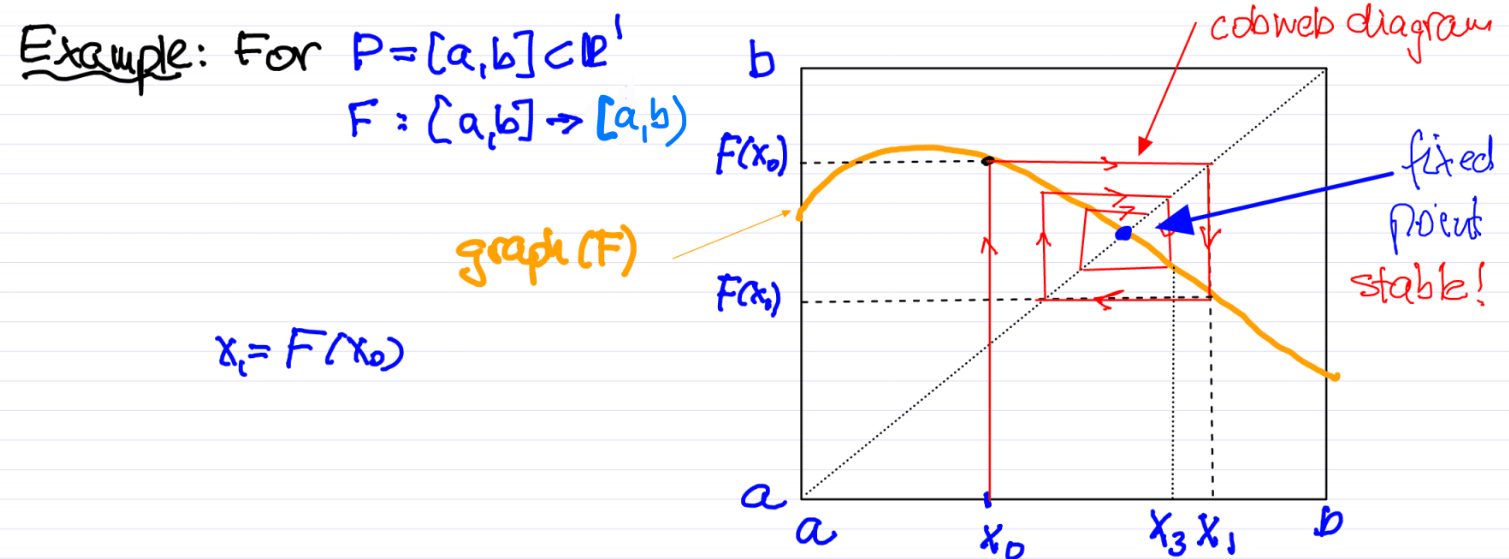
\includegraphics[width = \textwidth]{figures/intro/1DDS.png}
	\caption{Analysis of a one-dimensional system defined on the interval $x\in [a,b]$ using the cobweb diagram} \label{fig:cobweb}
\end{figure}
\end{ex}

\item In a CDS we have a first order system of ordinary differential equations (ODE)
	\begin{align}
		\boxed{
			\dot{ {x}} = f( {x},t)
		}
	\end{align}
	for $ {x}\in P$ and $t \in E$. This yields the initial value problem (IVP):
	\begin{align}
		\begin{dcases}
			\dot{ {x}} = f( {x},t) \\
			 {x}(t_0) =  {x}_0
		\end{dcases}
	\end{align}
	Assuming there exists a unique solution $\varphi(t; t_0,  {x}_0)$ with $\dot{\varphi} = f(\phi,t)$ and $\varphi(t_0)=  {x}_0$, then the following flow map is well defined
	\begin{align}
		\boxed{
		F_{t_0}^{t}( {x}_0) := \varphi(t; t_0,  {x}_0).}
	\end{align}

Geometrically, this solution can be viewed as a trajectory in phase space (cf. Fig. \ref{fig:cds_traj}).
	\begin{figure}[h!]
	\centering
	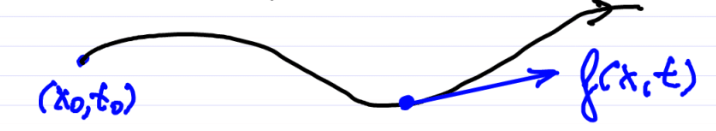
\includegraphics[width = 0.8\textwidth]{figures/intro/2CDS.png}
	\caption{Trajectory of a continuous dynamical system. The RHS is given by f(x,t), which is the tangent vector to this curve at the point $x$ at time $t$.} \label{fig:cds_traj}
	\end{figure}
	
	Such an $F_{t_0}^{t}$ has the properties
	\begin{enumerate}
		\item $F_{t_0}^{t}$ is as smooth as $f( {x},t)$,
		\item $F_{t_0}^{t_0} = I$ and $F_{t_0}^{t_2} = F_{t_1}^{t_2} \circ F_{t_0}^{t_1}$,
		\item $\left(F_{t_0}^{t}\right)^{-1} = F_{t}^{t_0}$ exists and is smooth.
\end{enumerate}
Properties (a) and (b) together are called the group property. A special case of continuous dynamical systems is the autonomous system.
\begin{align}
	\boxed{\dot{ {x}} = f( {x}).}	
\end{align}
The autonomy of a system implies
\begin{align}
	 {x}(s,t_0,  {x}_0) =  {x}(\underbrace{s-t_0}_{t}, 0,  {x}_0) \stackrel{!}{=}  {x}(t, {x}_0).
\end{align}
The induced flow map in this case is the one-parameter family of maps
\begin{align}
	\boxed{ F^{t} = F_{0}^{t}:  {x}_0 \mapsto  {x}(t, {x}_0).}
\end{align}
\end{enumerate}
\begin{ex}[Logisitic Equation]
	For a resource-limited population, we have the following dynamical system for $a> 0$, $b> 0$, and the population $x\in \mathbb{R}_+ \cup \{0\}$
	\begin{align}
		\dot{x} = ax(b-x).
	\end{align}
	In this case we have $E=\mathbb{R}$ and $\mathcal{F} = \{F^{t}\}_{t=-\infty }^{+\infty }$. This system has globally existing unique solutions (see later). We may analyze the behavior of this system by plotting $\dot{x}$ as a function of $x$, analogously to the cobweb diagram. This is demonstrated in Fig. \ref{fig:cds_analysis}. At $x$ values, where $\dot{x}$ is positive $x(t)$ is growing, while at negative values it is decreasing. This means, that fixed points, at which $x(t)=$ const. correspond to intersections of the graphs with the horizontal axis.
	\begin{figure}[h!]
		\centering
		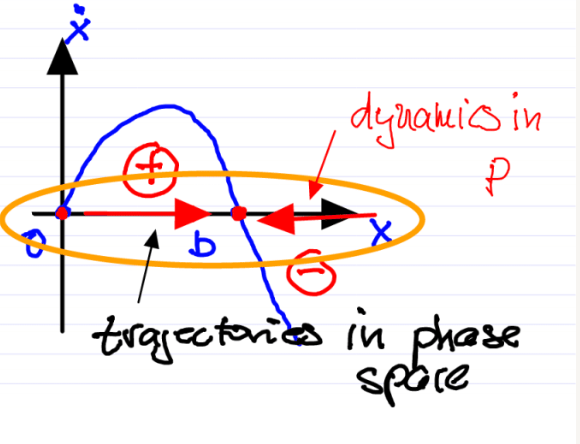
\includegraphics[width=0.4\textwidth]{figures/intro/3RHS.png}	
		\hspace{0.05\textwidth}
		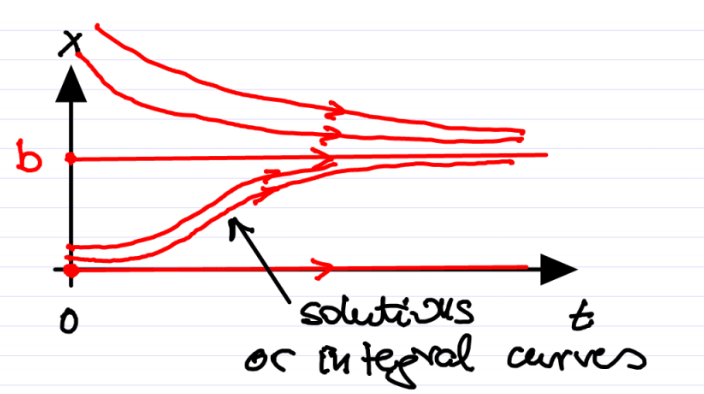
\includegraphics[width=0.4\textwidth]{figures/intro/4solutions.png}
		\caption{Left: Analysis of the right hand side. Right: Evolution in the extended phase space $P \times \mathbb{R}$.} \label{fig:cds_analysis}
	\end{figure}

\end{ex}

\begin{ex}[Pendulum]
Given the equation of motion
\begin{align}
	ml^2 \ddot{\varphi} = -mgl \sin(\varphi).
\end{align}
We let $ x_1 = \varphi$ and $ {x}_2 =\dot{\varphi}$ to transform into the first-order ODE form
\begin{align}
	\begin{dcases}
	\dot{x}_1 = x_2 \\
\dot{x}_2 = - \frac{g}{l} \sin (x_1).
	\end{dcases}
\end{align}
Thus we have 
\begin{align}
 {x} = 
\begin{pmatrix}
	x_1 \\ x_2
\end{pmatrix}; \quad
f( {x}) = 
\begin{pmatrix}
	x_2 \\ - \frac{g}{l}\sin(x_1)	
\end{pmatrix}.
\end{align}
Qualitative analysis gives the following facts
\begin{itemize}
	\item $(x_1, x_2) = (0,0)$ and $(x_1, x_2) = (\pi , 0)$ are zeros of $f$.
	\item Energy is conserved, hence both small and large amplitude oscillations are expected.
	\item The function $f(x)$ has symmetries: it is invariant under the transformation $(x_1, x_2, t) \mapsto (x_1, -x_2, -t)$ and $(x_1, x_2, t) \mapsto (-x_1, x_2, -t)$. See the left panel of Fig. \ref{fig:pendulum_symm+traj}.
\end{itemize}
\begin{figure}[h!]
	\centering
	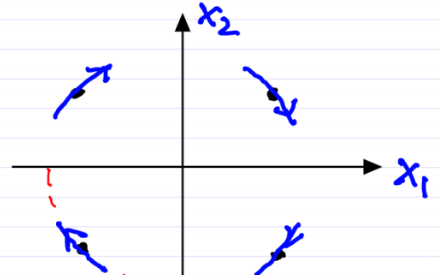
\includegraphics[width=0.4\textwidth]{figures/intro/6pendulum_symmetries.png}
	\hspace{0.05\textwidth}
	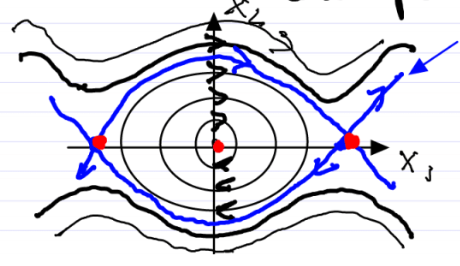
\includegraphics[width=0.4\textwidth]{figures/intro/5pendulum.png}
	\caption{Left: The symmetries of the dynamical system. Right: Phase portrait of the pendulum. Red dots show the fixed points, while the blue trajectories make up the separatrix.} \label{fig:pendulum_symm+traj}
\end{figure}
\begin{definition}
	A separatrix is a boundary (i.e. a codimension-1 surface) in phase space which separates regions of qualitatively different behaviors. In practice, it is unobservable by itself and connects different fixed points. The separatrix of the pendulum is shown in the right panel of Fig. 4.
\end{definition}

\end{ex}

\begin{ex}[Exploit geometry of phase space for analysis]
	Consider two cities, $A$ and $B$. The two cities are connected by two roads, denoted by the blue and green curves of the left panel of Fig. \ref{fig:two_cities}. We assume that travelling on the two roads, it is possible for two bikes to make it from $A$ to $B$ without ever being further away from each other than a distance $d<D$.

Assume two trucks are trying to make it between $A$ and $B$, on different roads in the opposite direction, carrying a load of width $D$. Given this information, can the trucks make it without hitting each other? We can view this problem as a continuous dynamical system with two coordinates $x_1$ and $x_2$ that parameterize the two routes between $A$ and $B$. This dynamical system is, in general, non autonomous.
	\begin{figure}[h!]
		\centering
		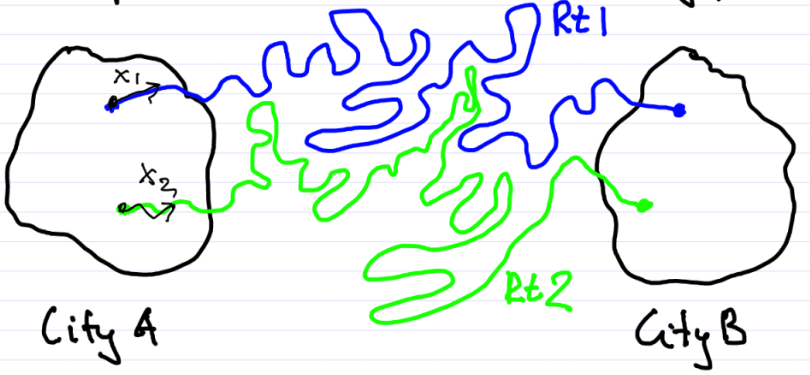
\includegraphics[width=0.5\textwidth]{figures/intro/7routes.png}
		\hspace{0.05\textwidth}
		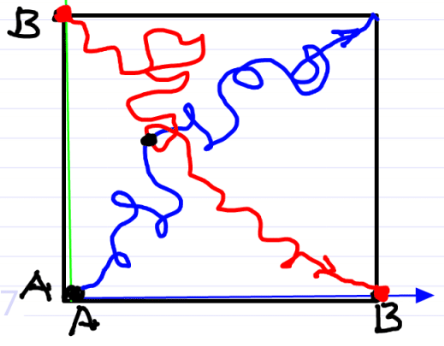
\includegraphics[width=0.3\textwidth]{figures/intro/8truck_geometry.png}
		\caption{Left: An example of the two bike routes. Right: Blue represents the trajectory of the two bikes, red represents the trajectory of the two trucks.} \label{fig:two_cities}
	\end{figure}

	The right panel of Fig \ref{fig:two_cities} shows the trajectories of the two trucks and the two bikes in phase space. The two trajectories must intersect by continuity, thus at that point the trucks must be at the same positions as the bikes, implying they are within distance $D$. Therefore the trucks must crash!	
\end{ex}



\newpage

\chapter{Fundamentals}
\section{Existence and uniqueness of solutions}
Consider  
\begin{align}
\begin{dcases}
	\dot{x} = f(x,t); & x \in \mathbb{R}^{n} \\
	x(t_0) = x_0
\end{dcases}.
\end{align}
Does this initial value problem have a unique solution? We have the following theorems to help us answer that question.
\begin{theorem}[Peano]
	\label{thm:Peano}
	If $f\in C^0$ near $(x_0, t_0)$, then there exists a local solution $\varphi(t)$, i.e., 
\begin{align}
	\dot{\varphi}(t) = f(\varphi(t), t), \varphi(t_0) = x_0;\ \forall  t\in (t_0 - \epsilon, t_0 + \epsilon);\ 0<  \epsilon \ll 1.
\end{align}
\end{theorem}
\begin{ex}[Free falling mass]
	We have that the total energy is conserved
	\begin{align}
		\frac{1}{2} m \dot{x}^2 = mg(x-x_0).
	\end{align}
This implies that
\begin{align}
	\begin{dcases}
		\dot{x} = \sqrt{2g(x-x_0)} \\
		x(0) = x_0
	\end{dcases}
\end{align}
on the set $P = \{ x \in \mathbb{R}:\ x \geq x_0\}$. Therefore we have that $f\in C^0$ in phase space, so by Peano's theorem (cf. \ref{thm:Peano}), there exists a local solution.
	\begin{figure}[h]
		\centering
		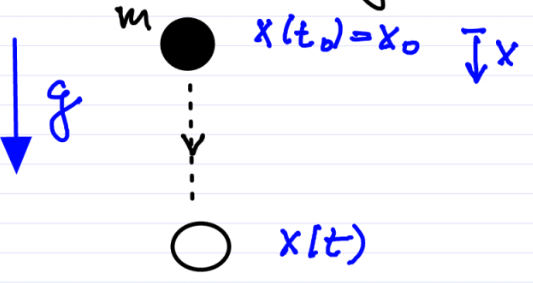
\includegraphics[width=0.4\textwidth]{figures/ch1/1freefall.png}
	\end{figure}
	The solution is actually $x(t) = x_0 + \frac{g}{2}(t-t_0)^2$, however $x(t) = x_0$ is also a solution to the IVP, therefore we do not have a unique solution. Physically there exists a solution, but this IVP was derived from a heuristic energy-principle, not from Newton's laws, which are not equivalent.
\end{ex}
\begin{definition}
A function is called locally Lipschitz around $x_0$ if there exists an open set $U_{x_0}$ and $L>0$ such that for all $x,y \in U_{x_0}$
\begin{align}
	\boxed{\left| f(y,t) - f(x,t)\right| \leq L |y - x|.}
\end{align}
\end{definition}

\begin{ex}[Lipschitz functions]
	Here we have an example of a Lipschitz and a non-Lipschitz function around $x_0$.
	\begin{figure}[h]
		\centering
		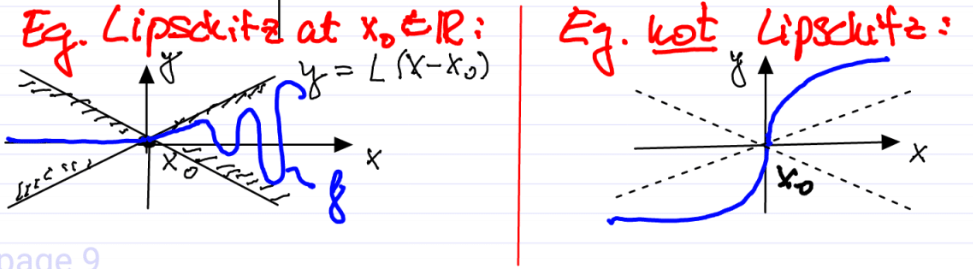
\includegraphics[width=0.8\textwidth]{figures/ch1/2lipschitz.png}
	\end{figure}
\end{ex}

\begin{theorem}[Picard]
	Assume 
	\begin{enumerate}
		\item  $f \in C^0$ in $t$ near $(t_0, x_0)$,
		\item $f$ is locally Lipschitz in $x$ near $(t_0, x_0)$.
	\end{enumerate}
	Then there exists a unique local solution to the IVP. The proof from Arnold's ODE. 	
\end{theorem}
\textbf{Note} $f$ is $C^1$ $\implies$ $f $ is Lipschitz $\implies $ $f$ is $C^0$.
\begin{ex}[Free falling mass revisted]
	We check if $f$ is Lipschitz.
	\begin{align}
		\frac{| f(x) - f(x_0) |}{|x-x_0|} = \frac{\sqrt{2g}}{\sqrt{|x-x_0|}} \not< L | x - x_0|.
	\end{align}
Thus $f$ is not Lipschitz near $x_0$.	
\end{ex}

\section{Geometric consequences of uniqueness}
If the solution is unique, we have a few facts that can be derived from the geometric point of view.
\begin{enumerate}
	\item The trajectories of autonomous systems cannot intersect. Note that fixed points do not violate this (e.g. pendulum equations).
		\begin{figure}[h]
			\centering
			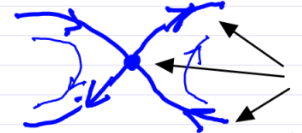
\includegraphics[width=0.3\textwidth]{figures/ch1/3pendulum_trajectories.png}
			\caption{The phase portrait of the pendulum. Trajectories do not intersect since each arrow is pointing at separate trajectories.}
		\end{figure}
		
	\item For non-autonomous systems, intersections in phase space are possible. In which case we can extend the phase space in order to get an autonomous system where there cannot be any intersections.
		\begin{align}
			X = 
			\begin{pmatrix}
				x \\ t
			\end{pmatrix},\
			F(X) = 
			\begin{pmatrix}
				f(x,t) \\ 1
			\end{pmatrix};\
			\dot{X} = F(X).
		\end{align}
		\begin{figure}[h]
			\centering
			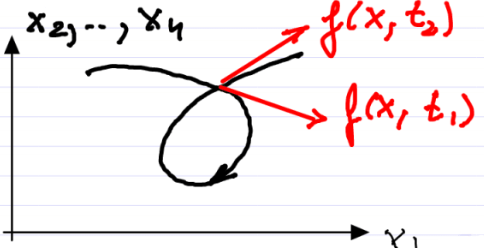
\includegraphics[width=0.4\textwidth]{figures/ch1/4intersecting_trajectories.png}
			\hspace{0.05\textwidth}
			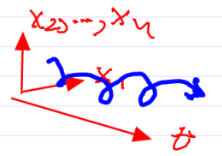
\includegraphics[width=0.3\textwidth]{figures/ch1/5extended_space.png}
			\caption{Left: Intersecting trajectories in phase space for a non-autonomous system. Right: The same trajectory in the extended phase space, without intersections.}
		\end{figure}
\end{enumerate}

\section{Local vs global existence}
\begin{ex}[Exploding solution]
	\begin{align}
		\begin{dcases}
			\dot{x} = x^2 \\
			x(t_0) = 1.
		\end{dcases}
	\end{align}
	Integrating yields the solution $x(t) = \frac{1}{1 - (t-t_0)}$. This solution blows up at $t_{\infty }=t_0 + 1$, therefore the solution is only local.	
\begin{figure}[h]
\centering	
\begin{tikzpicture}
	\begin{axis}
		[xmin=0, xmax=2.5, ymin=0.5, ymax=3, domain = 1:1.9, xlabel=$t$, ylabel=$x(t)$, xtick=\empty, ytick=\empty]
		\addplot[color=black] {1/(2-x)};
		\addplot[color=black, dashed] coordinates {(1.7,0.5) (1.7,3.1)} node[pos=0, above right] {$t_{\infty }$};
		\addplot[color=black, dashed] coordinates {(1,0.5) (1,1)} node[pos=0, above right] {$t_{0}$};
		\addplot[color=black, dashed] coordinates {(0,1) (1,1)} node[pos=0, above right] {$x_{0}$};
	\end{axis}
\end{tikzpicture}
\end{figure}
\end{ex}

\begin{theorem}[Continuation of solution]
	If a local solutions cannot be continued to to a time $T$, then we must have
	\begin{align}
		\boxed{\lim_{t\to T} |x(t)|= \infty.}
	\end{align}
The proof from Arnold's ODE.	
\end{theorem}

\begin{ex}[Coupled Pendulum System]
	We set $x_1 = \varphi_1,\ x_2 = \dot{\varphi_1},\ x_3 = \varphi_2,\ x_4=\dot{\varphi_2} $ and get the following equation of motion
\begin{align}
	\begin{dcases}
		\dot{x}_1 = x_2 \\ \dot{x}_2 = \ldots \\ \dot{x}_3 = x_4 \\ \dot{x}_4 = \ldots
	\end{dcases}
\end{align}
The RHS is smooth, therefore there exists a unique local solution to any IVP.
\begin{figure}[h]
	\centering
	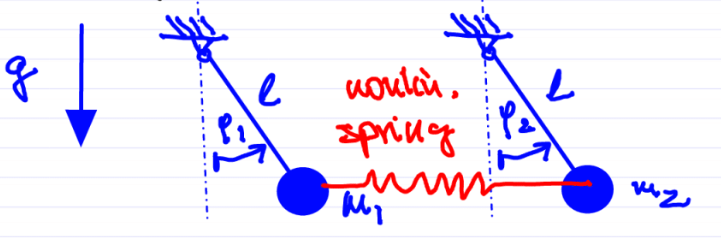
\includegraphics[width=0.6\textwidth]{figures/ch1/6coupled_pendulum.png}
	\caption{Physical setup of the coupled pendulum with a nonlinear spring.}
\end{figure}
The phase space is given by 
\begin{align}
	P = \{x:\ x_1 \in S^1,\ x_2 \in \mathbb{R},\ x_3 \in S^1,\ x_4 \in \mathbb{R} \} = S^1 \times \mathbb{R}\times S^1 \times \mathbb{R}.
\end{align}
Where $S^1$ is the 1 dimensional sphere (i.e. a circle). With this space we know that $|x_1|$ and $|x_3|$ are bounded. Due to energy being conserved we have
\begin{align}
	E &= T+V = \frac{1}{2}m_1 l_1 x_2^2 + \frac{1}{2}m_2 l_2 x_4^2 + \underbrace{V(x_1, x_3)}_{\geq 0}\\
	E &= E_0 =  \textrm{constant} \geq 0.
\end{align}
Hence $|x_2|$ and $|x_4|$ are also bounded, therefore all solutions exist globally.
\end{ex}
\begin{definition}
	A linear system is one such that for $x\in \mathbb{R}^{n},\ A(t) \in \mathbb{R}^{n\times n}$ and $A\in C^0$ 
	\begin{align}
		\boxed{\dot{x} = A(t) x.}
	\end{align}
\end{definition}

\begin{remark}[]
	Note that  $S = \frac{1}{2}(A + A^T)$ is symmetric (i.e. $S = S^T)$ and $\Omega = \frac{1}{2}(A - A^T)$ is skew symmetric (i.e. $\Omega = -\Omega^T$). Furthermore the eigenvalues of $S$, $\lambda_i$, are all real and their respective eigenvectors, $e_i$, are orthogonal.
\end{remark}

\begin{ex}[Global existence in linear systems]
\begin{align}
	\langle x, \dot{x} \rangle &= \frac{1}{2} \frac{d}{dt} |x(t)|^2 = \langle x, A(t) x\rangle = \langle x, (S(t) + \Omega(t) ) x \rangle \\
				   &= \langle x, S(t) x \rangle + \underbrace{\langle x, \Omega(t) x \rangle}_{=0} \stackrel{(*)}{=} 
				   \sum_{i=1}^{n} \lambda_i(t) x_i^2 \\
				   &\leq \lambda_{ \textrm{max} }(t) \sum_{i=1}^{n} x_i^2 = \lambda _{ \textrm{max} }(t) | x(t)|^2.
\end{align}
Where in $(*)$ we used that $x = \sum_{i=1}^{n} x_i e_i $ with $|e_i|=1$ and $e_i \perp e_j$ for all $i \neq j$. Thus we get
\begin{align}
	\frac{\frac{1}{2}\frac{d}{dt}|x(t)|^2}{|x(t)|^2} \leq \lambda_{ \textrm{max} }(t) 
	\implies \int_{t_0}^{t} \log \left( \frac{|x(s)|^2}{|x(t_0)|^2} \right) ds \leq \lambda _{ \textrm{max} }(s) ds.
\end{align}
By exponentiating both sides, we obtain
\begin{align}
\boxed{ |x(t)| \leq |x(t_0) | \exp\left(\int_{t_0}^{t} \lambda_{ \textrm{max} }(s)ds\right).}
\end{align}
Therefore, by the continuation theorem, global solutions exist as long as $\int_{t_0}^{t} \lambda_{ \textrm{max} }(s) ds < \infty $.
\end{ex}

\section{Dependence on initial conditions}
Given the IVP
\begin{align}
	\begin{dcases}
	\dot{x} = f(x,t) \\ x(t_0) = x_0.
	\end{dcases}
\end{align}
With $x \in \mathbb{R}^{n}$ and $f\in C^r$ for some $r\geq 1$, we have the solution $x(t; t_0, x_0)$.
\textbf{Question} How does the solution depend on initial data?
But first, why do we care about this? Because we robust solutions with respect to errors and uncertainties in the initial data.
\begin{theorem}[]
	If $f \in C^r$ for $r\geq 1$ then $x(t; t_0, x_0)$ is $C^r$ in $(t_0, x_0)$. Proof in Arnold's ODE.
\end{theorem}

The geometric meaning of this is that for $U \subset P \subset \mathbb{R}^{n}$ we have that $F_{t_0}^{t}(U)$ is a smooth deformation of $U$.
\begin{figure}[h]
	\centering
	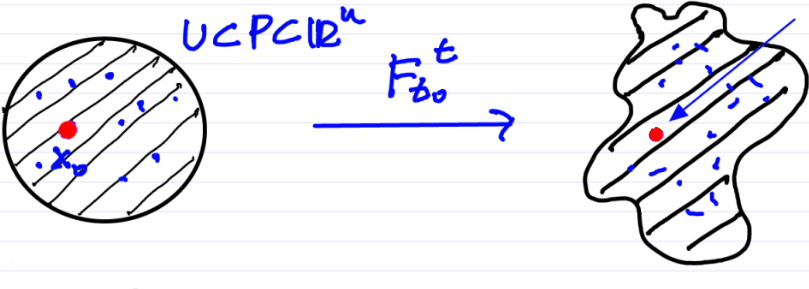
\includegraphics[width=0.7\textwidth]{figures/ch1/7smooth_transform.png}
	\caption{The smooth transformation of $U$. The red point on the right it $F _{t_0}^t(x_0)$, i.e. the image of $x_0$ through the evolution operator.}
\end{figure}
It turns out $\left(F_{t_0}^{t}\right)^{-1} = F_{t}^{t_0}$ is also $C^r$, hence we have that $F_{t_0}^{t}$ is a diffeomorphism. 

Now, how can we compute the Jacobian of the flow map $\frac{\partial x(t; t_0, x_0)}{ \partial x_0} = DF _{t_0}^{t}(x_0)$? We will use the IVP.
\begin{align}
	\frac{d}{dt}\frac{\partial x}{\partial x_0} = D_x f(x(t; t_0, x_0), t) \frac{\partial x}{\partial x_0}.
\end{align}
The flow gradient satisfies the IVP
\begin{align}
	\frac{d}{dt}\left[ DF_{t_0}^{t}(x_0)\right] &= D_{x}f(F_{t_0}^{t}(x_0), t) DF_{t_0}^{t}(x_0) \\
	DF_{t_0}^{t_0}(x_0) &= I.
\end{align}
This gives us the equation of variations (linear, non-autonomous)
\begin{align}
	\begin{dcases}
		\dot{M} = D_x f(x(t; t_0, x_0)) M \\ M(t_0) = I.
	\end{dcases}
\end{align}

\begin{ex}[Locations of extreme deformation in phase space]
	We define 
	\begin{align}
		\xi(t) &:= \tilde{x}(t) - x(t) = x(t; t_0, \tilde{x_0}) - x(t; t_0, x_0)\\
		       &= x(t; t_0, x_0) + \frac{\partial x}{\partial x_0}(t; t_0, x_0)\xi_0 + \mathcal{O}(|\xi_0|^2) - x(t; t_0, x_0) \\
		       &= DF_{t_0}^{t}(x_0)\xi_0 + \mathcal{O}(|\xi_0|^2).
	\end{align}
	Where we used the Taylor expansion and assume the perturbation to $x_0$ is small, i.e. $|\xi_0| \ll 1$.
	\begin{figure}[h]
		\centering
		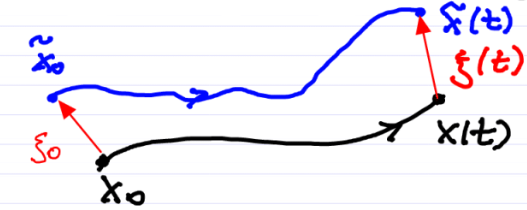
\includegraphics[width=0.5\textwidth]{figures/ch1/8dispersion.png}
	\end{figure}
	Therefore we have
	\begin{align}
		|\xi(t)|^2 &= \langle DF_{t_0}^{t}(x_0) \xi_0, DF_{t_0}^{t}(x_0)\xi_0 \rangle + \mathcal{O}(|\xi_0|^3) \\
			   &= \langle \xi_0, \underbrace{\left[ DF_{t_0}^{t}(x_0) \right]^T DF_{t_0}^{t}(x_0)}_{=: C_{t_0}^{t}(x_0)} \xi_0 \rangle + \mathcal{O}(|\xi_0|^3).
	\end{align}
	$C_{t_0}^{t}(x_0)$ is known as the Cauchy-Green strain tensor (field of $n\times n$ symmetric matrices).
	Therefore the largest possible deformation is
	\begin{align}
		\max_{x_0, xi_0} \frac{|\xi(t)|^2}{|\xi_0|^2} = \max_{x_0, \xi_0}\frac{\langle \xi_0, C_{t_0}^{t}(x_0) \xi_0 \rangle}{|\xi_0|^2} = \max_{x_0} \lambda_{n}(x_0).
	\end{align}
	Where we used that $C_{t_0}^{t}$ is positive definite in the last equality, and that $\lambda_n(x_0)$ is the largest eigenvalue of $C_{t_0}^{t}(x_0)$. We typically have exponential growth.	
\end{ex}
\begin{definition}
	The finite-time Lyapunov exponent is defined as
	\begin{align}
		\boxed{ \textrm{FTLE} _{t_0}^{t}(x_0) := \frac{1}{2(t-t_0)} \log(\lambda_n(x_0)).}
	\end{align}
\end{definition}
The FTLE is a diagnostic quantity for Lagrangian Coherent Structure (LCS), i.e. influential surfaces governing the evolution in $P$.
\begin{figure}[h]
	\centering
	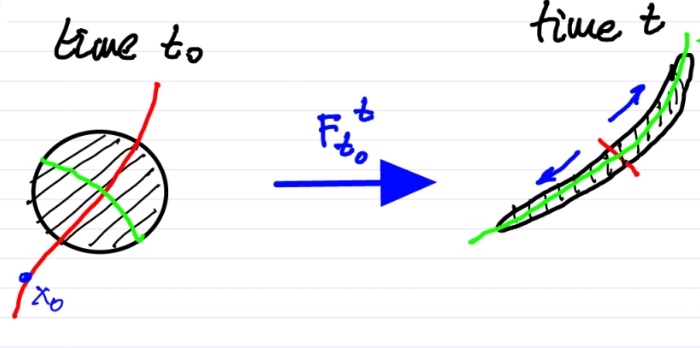
\includegraphics[width=0.6\textwidth]{figures/ch1/9deformation.png}
	\caption{On the left the red ridge represents large values of $ \textrm{FTLE} _{t_0}^{t}$, on the right the green ridge the high values of $ \textrm{FTLE} _{t}^{t_0}$.}
\end{figure}
\begin{figure}[h]
	\centering
	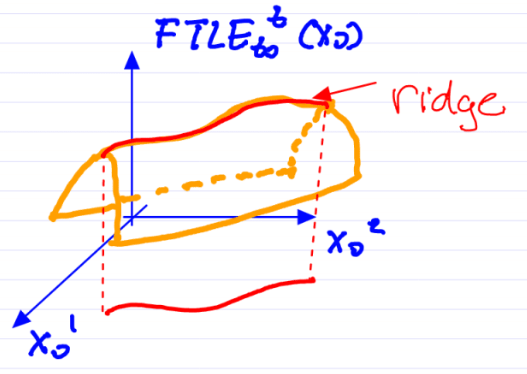
\includegraphics[width=0.4\textwidth]{figures/ch1/10ridge_projection}
	\caption{The projection of the FTLE ridge onto the initial value space.}
\end{figure}

The ridges of $ \textrm{FTLE} _{t_0}^{t}$ are the repelling LCS, meanwhile the ridges of $ \textrm{FTLE} _{t}^{t_0}$ are the attracting LCS. Now we are left with the problem of computing $F_{t_0}^{t}(x_0)$. Recall that analytically we start with $F_{t_0}^{t}(x_0)$ and use this to calculate $DF_{t_0}^{t}(x_0)$. From here we can find $C_{t_0}^{t}(x_0)$, giving us $\lambda_n(x_0)$ and thereby the FTLE. We know approximate this process numerically.
\begin{enumerate}
	\item Define an initial $M\times N$ grid of initial data $x_0(i,j) \in \mathbb{R}^2$.
	\item Launch trajectories numerically from grid points to obtain a discrete approximation of $F_{t_0}^{t}(x_0)$ as $F_{t_0}^{t}(x_0(i,j))$.
	\item Use finite differencing to approximate $DF_{t_0}^{t}(x_0(i,j)).$
\end{enumerate}

\begin{ex}[Double gyre model using FTLE]
We have the stream function
\begin{align}
	\Psi(x,y) = -\sin(\pi x) \sin(\pi y).
\end{align}
This gives the fluid velocity field
\begin{align}
	V = 
	\begin{dcases}
		\dot{x} = \frac{\partial \Psi}{\partial y} \\
		\dot{y} = - \frac{\partial \Psi}{\partial x}.
	\end{dcases}
\end{align}
\begin{remark}[]
This is an example of a Hamiltonian system of $\Psi$ being the Hamiltonian $H$.
\end{remark}
For any autonomous Hamiltonian system we have that $H$ is constant along trajectories, we check
\begin{align}
	\frac{d}{dt}\Psi(x(t),y(t)) = \frac{\partial \Psi}{\partial x}\dot{x} + \frac{\partial \Psi}{\partial y}\dot{y} = 0.
\end{align}
So we have that trajectories are level curves of $\Psi(x,y)$. We can then derive the phase portrait from the level curves of $\Psi$. Further, we have that $\dot{x} = \frac{\partial \Psi}{\partial y} = - \pi \sin(\pi x) \cos(\pi y)$ which yields that $ \textrm{sign} (\dot{x}) = -  \textrm{sign} (\sin(\pi x))  \textrm{sign} (\cos(\pi y))$. Putting these together we can construct the contour plot with arrows.

\begin{figure}[h]
	\centering
	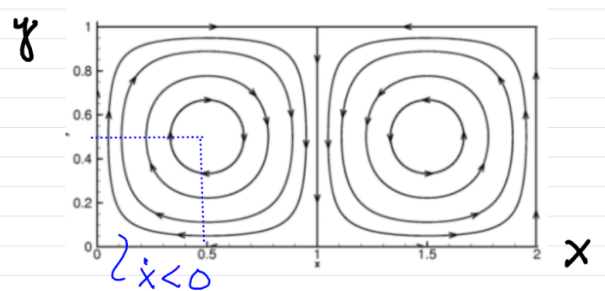
\includegraphics[width=0.5\textwidth]{figures/ch1/11contour_phase.png}
	\hspace{0.03\textwidth}
	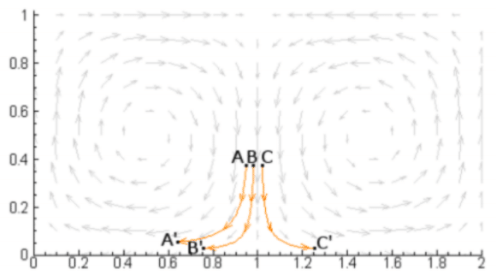
\includegraphics[width=0.45\textwidth]{figures/ch1/12ftle_exploration.png}
	\caption{}
	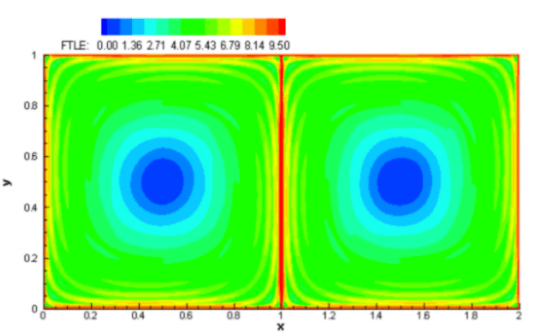
\includegraphics[width=0.5\textwidth]{figures/ch1/13ftle_final.png}
	\caption{Top left: The analytic phase plot. Top right: The exploration done to calculate FTLE. Bottom: The FTLE plot.}
\end{figure}
Figures here were taken from Shawn Shadden of UC Berkely.
\end{ex}

\begin{ex}[ABC flow]
	Let our dynamic system be defined as follows with $A,B,C \in \mathbb{R}$
\begin{align}
	\begin{dcases}
		\dot{x} = A \sin(z) + C \cos(y) \\
		\dot{y} = B \sin(x) + A \cos(z) \\
		\dot{z} = C \sin(y) + B \cos(x).
	\end{dcases}
\end{align}
We are looking for an exact solution of Euler's equation of inviscid fluids. We have an autonomous velocity field, which is known to generate chaotic fluid trajectories.
\begin{figure}[h]
	\centering
	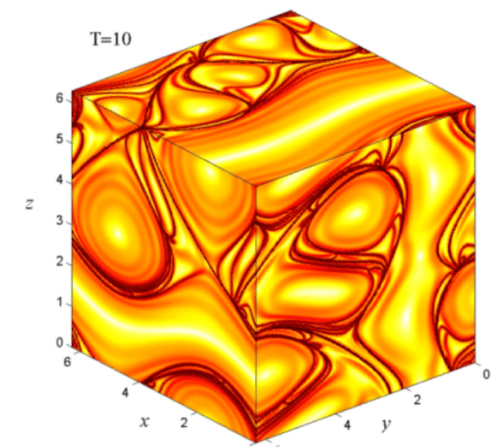
\includegraphics[width=0.4\textwidth]{figures/ch1/14fluid1.png}
	\hspace{0.03\textwidth}
	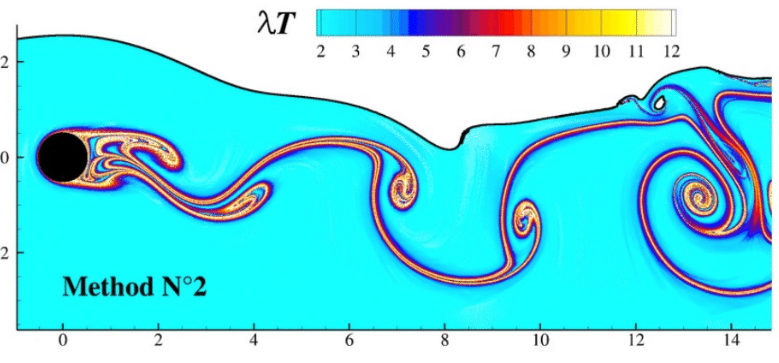
\includegraphics[width=0.55\textwidth]{figures/ch1/15vortex_shedding.png}
	\caption{Left: numerical results of dynamic system (Guckenheimer-Holmes Physica D, 2001). Right: vortex shedding behind a cylinder under a free surface (Sun et. al, 2016).}
\end{figure}
\end{ex}
\vfill
\section{Dependence on parameters}
We now have the IVP
\begin{align}
	\begin{dcases}
		\dot{x} = f(x,t, \mu ) \\ x(t_0) = x_0.
	\end{dcases}
\end{align}
With $x \in \mathbb{R}^{n},\ f\in C^r,\ r\geq 1$, therefore we have a solution $x(t; t_0, x_0, \mu ) \in C^r_{x_0}$.

\textbf{Question} How does the solution depend on $\mu $? 
\textbf{Why Care?} We would like robustness of solutions with respect to parameter changes or uncertainties in the model.
\begin{ex}[Perturbation Theory]
Given a weakly nonlinear oscillator
\begin{align}
	m \ddot{x} + c \dot{x} + kx = \epsilon f(x, \dot{x}, t),\ 0 \leq \epsilon \ll 1,\ x \in \mathbb{R}.
\end{align}
The usual approach is to seek solutions by expanding from known solution of the linear limit, i.e.
\begin{align}
	x_{\epsilon}(t) = \varphi_0(t) + \epsilon \varphi_1(t) + \epsilon^2 \varphi_2(t) + \ldots + \mathcal{O}(\epsilon^r).
\end{align}
If $x_{\epsilon}(t)$ is in $C^{r}_{\epsilon}$, we have $\varphi_1(t) = \left.\frac{\partial x_\epsilon(t)}{\partial \epsilon}\right|_{\epsilon =0}$ and $\varphi_2(t) = \left.\frac{\partial^2 x_\epsilon(t)}{\partial \epsilon^2}\right|_{\epsilon =0}$
\end{ex}

\textbf{Answer} Regularity with respect to $\mu $ actually follows from regularity with respect to $x_0$. Use the trick of extending the IVP with a dummy variable $\mu $ 
\begin{align}
	\begin{dcases}
		\dot{x} = f(x,t,u) \\ \dot{mu} = 0 \\ x(t_0) = x_0 \\ \mu (t_0) = mu_0.
	\end{dcases}
\end{align}
Thus with $X=
\begin{pmatrix}
	x \\ \mu 
\end{pmatrix}
\in \mathbb{R}^{n+p}$ and $F(X_0) = 
\begin{pmatrix}
	f \\ 0
\end{pmatrix};\ X_0 = 
\begin{pmatrix}
	x_0 \\ \mu _0
\end{pmatrix}
$. Therefore we have
\begin{align*}
	\begin{dcases}
		\dot{X} = F(X) \\ X(t_0) = X_0
	\end{dcases} \numberthis \label{eq:ivp_param}
\end{align*}
Applying the previous result on regularity with respect to $x_0$ to \eqref{eq:ivp_param}, we have that $f\in C^{r}_{x,\mu }$ implies that $X(t) \in C^{r}_{X_0}$ in turn implying that $x(t; t_0, x_0, \cdot) \in C^{r}_{\mu }$. The solution is as smooth in parameters as the RHS of the dynamic system.


\newpage

\chapter{Stability of fixed points}
Now we would like to begin to explore the behaviour of dynamical systems around fixed points. This will allow us to find out if we should expect to observe a fixed state, and to understand what happens if we perturb the system away from this fixed state.
\section{Basic definitions}
Consider
\begin{align}
	\dot{ {x}}=f( {x},t),\  {x} \in \mathbb{R}^{n},\ f\in \mathcal{C}^{1}.
\end{align}
Assume that $ {x}=0$ is a fixed point, i.e. $f({0},t) = {0}$ for all $t \in \mathbb{R}$. If the fixed point is originally at ${x}_0\neq {0}$, shift it to zero by letting $\tilde{ {x}}:= {x}- {x}_0$, therefore 
\begin{align}
	\dot{\tilde{ {x}}} = \dot{ {x}} = f( {x}_0 + \tilde{ {x}}, t) = \tilde{f}(\tilde{ {x}}, t).
\end{align}
We would like to understand how the dynamical system behaves near its equilibrium state. To this end we introduce the following definitions.
\begin{definition}[Lyapupnov Stability] \label{def:stable}
	The fixed point $ {x}={0}$ is stable if for all $t_0$, for all $\varepsilon>0$ small enough, there exists a $\delta=\delta(t_0, \varepsilon)$, such that for all $ {x}_0 \in \mathbb{R}^{n}$ with $\| {x}_0\| \leq \delta$, we have 
	\begin{align}
		\boxed{
			\left \|  {x}(t;t_0,  {x}_0) \right\| \leq \varepsilon \quad \forall t \geq t_0.
		}
	\end{align}
\begin{figure}[h!]
	\centering
	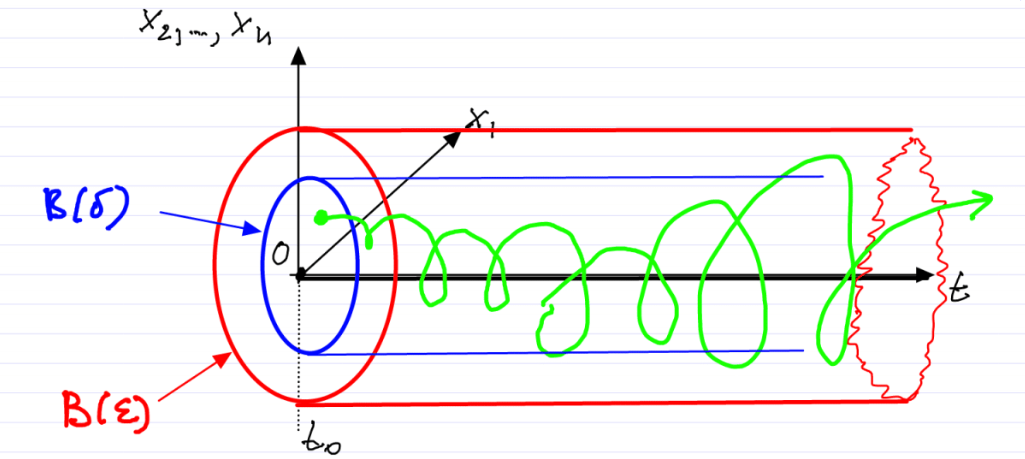
\includegraphics[width=0.7\textwidth]{figures/ch2/1lyapunov_stability.png}
	\caption{An example such a $\delta$ for a given Lyapunov stable fixed point.}
	\label{fig:lyapunov_stability_def}
\end{figure}
\end{definition}
\begin{remark}[N-dimensional ball]
	When writing $\mathcal{B}(r)$ we refer to the ball of radius $r$ in $\mathbb{R}^{n}$, i.e. the set $\{x:\ \|x\| < r\}$.
\end{remark}

\begin{ex}[Stability of the lower equilibrium of the pendulum]
	Recall the equation of motion of the pendulum $\ddot{\varphi} + \sin(\varphi) = 0$, that we transform into a first order ODE by setting $x_1 = \varphi$ and $x_2 = \dot{\varphi}$ to obtain
	\begin{align}
		\begin{dcases}
		\dot{x}_1 = x_2 \\
	\dot{x}_2 = -\sin(x_1).
		\end{dcases}
	\end{align}
	For small $\varepsilon>0$, this geometric procedure gives a $\delta(\varepsilon)>0$ such that the definition of stability is satisfied for $ {x}=0$. We can see in Fig. \ref{fig:pend_lower_stability} that for any initial point chosen within the blue circle, it's trajectory remains within the red circle for all time (cf. Fig. \ref{fig:lyapunov_stability_def}). Therefore $ {x}=0$ is (Lyapunov) stable.
	\begin{figure}[h!]
		\centering
		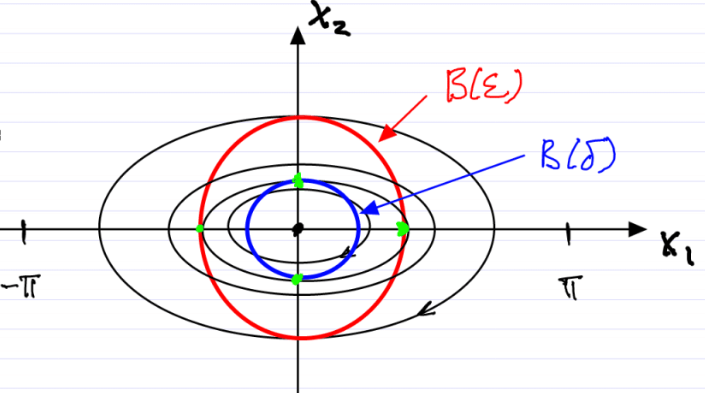
\includegraphics[width=0.5\textwidth]{figures/ch2/2pendulum_stability.png}
		\caption{Stability of lower equilibrium for the pendulum, here $0<\varepsilon<\pi $.}
	\label{fig:pend_lower_stability}
	\end{figure}
\end{ex}

\begin{definition}[Asymptotic stability]
	The fixed point $ {x}=0$ is \emph{asymptotically stable} if
\begin{enumerate}
	\item it is stable,
	\item for all $t_0$, there exists $\delta_0(t_0, \varepsilon)$ such that for every $ {x}_0$ with $\|  {x}_0 \| \leq \delta_0$ we have
		\begin{align}
			\boxed{\lim_{t\to \infty }  {x}(t; t_0,  {x}_0) = 0.}
		\end{align}
\end{enumerate}
\begin{figure}[h!]
	\centering
	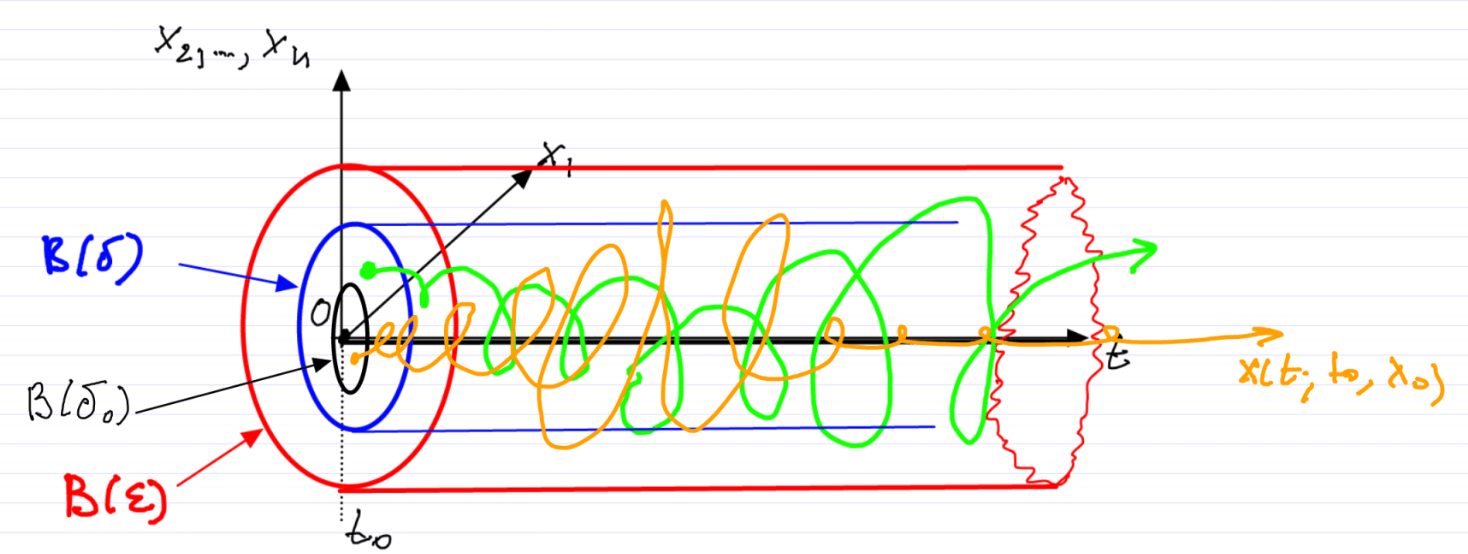
\includegraphics[width=0.7\textwidth]{figures/ch2/3asymp_stability.png}
	\caption{An example for an asymptotically stable fixed point (black trajectory).}
\end{figure}
\end{definition}

\begin{definition}[Domain of attraction] 
	The \emph{domain of attraction} of the fixed point $x=0$ is the set of all $ {x}_0$'s for which
	\begin{align}
		\boxed{\lim_{t\to \infty } {x}(t;t_0,  {x}_0)=0. }	
	\end{align}
	
\end{definition}

\begin{ex}[Damped pendulum]
	We have the equation of motion with the linear damping coefficient $c$
	\begin{align}
		\ddot{\varphi} + c \dot{\varphi} + \sin(\varphi) = 0,\quad c>0.
	\end{align}
	Transforming into a first-order ODE with $x_1 = \varphi$ and $x_2 = \dot{\varphi}$ gives
	 \begin{align}
		\begin{dcases}
		\dot{x}_1 = x_2\\ \dot{x}_2 = -cx_2 - \sin(x_1).
		\end{dcases}
	\end{align}
The total energy is given by
\begin{align}
	E = \frac{1}{2}x_2^2 + \left( 1 - \cos(x_1) \right). 
\end{align}
Further we have the rate of energy change
\begin{align}
\frac{d}{dt} E(x_1(t), x_2(t)) = x_2 \left(\dot{x}_2 + \sin(x_1) \right) = -c x_2^{2}.
\end{align}
\begin{figure}[h!]
	\centering
	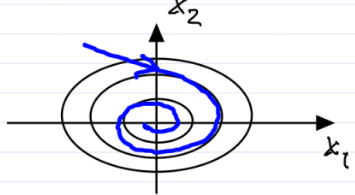
\includegraphics[width=0.35\textwidth]{figures/ch2/4damped_pendulum.png}
	\caption{An example of a trajectory which loses energy, in this case due to damping.}
	\label{fig:losing_energy_pend}
\end{figure}

Therefore, along trajectories energy decreases monotonically as shown in Fig \ref{fig:losing_energy_pend}. By the $\mathcal{C}^0$ dependence of the trajectory on initial conditions, the trajectories remain close to the undamped oscillations for small $c>0$. We conclude that trajectories are inward spirals for a small dissapation $c>0$. The fixed point $ {x}=0$ is still Lyapunov stable, but asymptotic stability does not yet follow (is the limit of $ {x}(t)$ equal to 0?).
\begin{remark}[LaSalle's invariance principle]
	This conclusion follows rigorously from LaSalle's invariance principle, namely if we assume that $\dot{ {x}}=f( {x})$, $f \in \mathcal{C}^1$, and that there exists a $V\in \mathcal{C}^1$ with 
	\begin{align}
		\dot{V} = \frac{dV( {x}(t))}{dt} \leq 0.	
	\end{align}
	Then the set of accumulation points for any trajectory is contained in the set of trajectories that stay within the set $I=\{ {x} \in \mathbb{R}^{n}:\ \dot{V}( {x}) = 0\}$.
\end{remark}
\end{ex}

\begin{ex}[]
	Consider the following dynamical system in polar coordinates, i.e. $r\cos(\theta) = x$ and $r \sin(\theta) = y$,
	\begin{align}
		\begin{dcases}
			\dot{r} = r(1-r) \\ \dot{\theta} = \sin^2\left( \frac{\theta}{2} \right).
		\end{dcases}
	\end{align}
	Note that $r=0$ is a fixed point, the set $r=1$ is an invariant circle, and the set $\theta=0$ is an invariant set. An invariant set is a set such that if the dynamical system is started on the set, it remains in the set for all time. Examining the radial evolution reveals that the equation of motion decouples. We see that $\dot{\theta}\geq 0$, so rotation is either positive or null.
	\begin{figure}[h!]
		\centering
		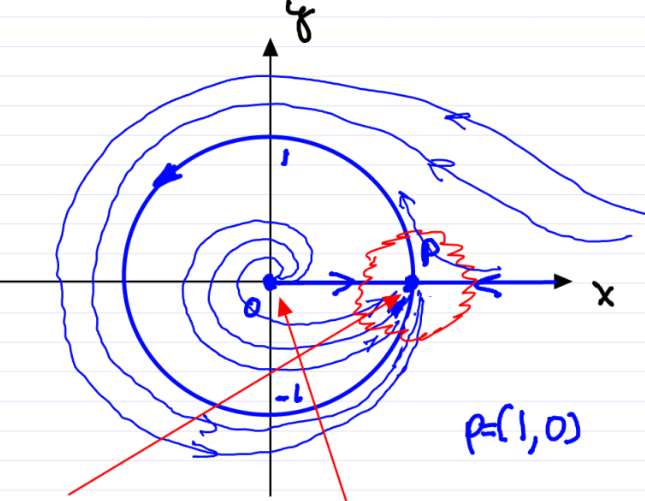
\includegraphics[width=0.5\textwidth]{figures/ch2/5polar_cds.png}
		\caption{Phase portrait of the dynamical system in cartesian coordinates, with the red arrows pointing to the two unstable equilibria.}
		\label{fig:polar_attractor}
	\end{figure}

	 From Fig. \ref{fig:polar_attractor} we can see that both of the fixed points, $(0,0)$ and $(1,0)$, are not stable. However, inspecting Fig. \ref{fig:polar_attractor} we see that that $p=(1,0)$ is an example of an attractor: a set with an open neighborhood of points that all approach the set as $t\to \infty $.
\end{ex}

\begin{definition}[Invariant set]
	The set $S \subset P$ is an \emph{invariant set} for the flow map $F^{t}:P \to P$ if $F^{t}(S) =S$ for all $t \in \mathbb{R}$.
\end{definition}

\begin{definition}[Unstable point]
	A fixed point $ {x}=0$ is unstable if it is not stable.
\end{definition}

\begin{remark}[]
	We can negate a mathematical statement by using the reverse relational operators outside the statements involving these operators i.e. $ \exists \to \forall $ and $\forall \to \exists $. For example we have for continuity $\forall \varepsilon\ \exists \delta:\  \|f( {x}) - f( {y}) \| < \varepsilon$ if $ \| {x}- {y} \|<\delta$, meanwhile for discontinuity we have  $\exists \varepsilon:\ \forall \delta:\  \|f( {x}) - f( {y}) \| \geq  \varepsilon$ for $ \| {x}- {y} \|< \delta$.

	In our case for stability we have
	\begin{align}
		\forall \varepsilon,t_0: \quad \exists \delta>0: \quad \forall  {x}_0  \textrm{ with }  \| {x}_0 \| < \delta: \quad  \| {x}(t) \|\leq \varepsilon \quad \forall t\geq t_0.
	\end{align}
Meanwhile for instability 
\begin{align}
	\exists \varepsilon,t_0:\quad \underbrace{\forall \delta>0}_{ \textrm{``for arbitrarily small"} }:\quad \exists  {x}_0  \textrm{ with }  \| {x}_0 \|<\delta: \quad  \| {x}(t) \|>\varepsilon \quad \underbrace{\exists t\geq t_0}_{ \textrm{``for some"} }.
\end{align}
This negation is demonstration in Fig. \ref{fig:instable_def}.
\begin{figure}[h!]
	\centering
	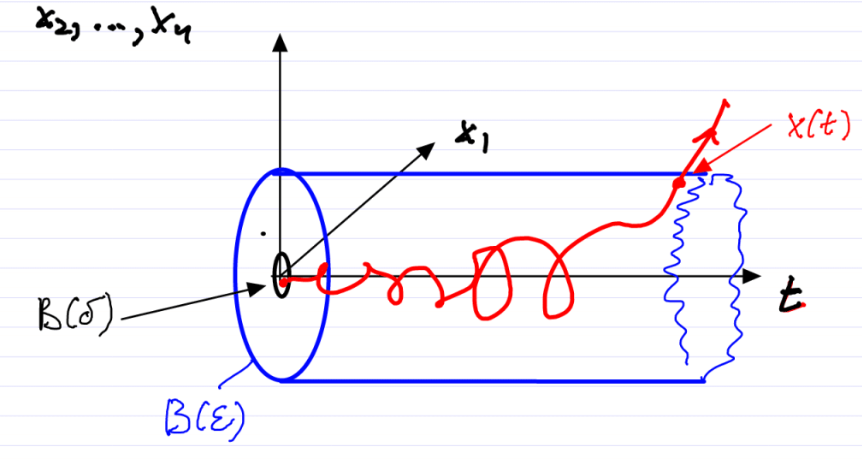
\includegraphics[width=0.5\textwidth]{figures/ch2/6unstable_def.png}
	\caption{Example of an unstable fixed point, with the red trajectory representing a trajectory starting arbitraritly close to the fixed point, leaving a given $\varepsilon$-ball.}
	\label{fig:instable_def}
\end{figure}
\end{remark}

\begin{remark}[]
	By $\mathcal{C}^0$ dependence of trajectories on initial conditions, if $ {x}(t;t_0, {x}_0)$ leaves $\mathcal{B}(\varepsilon)$, then for $\tilde{ {x}}_0$ close enough to $ {x}_0$, $ {x}(t;t_0,\tilde{ {x}}_0)$ also leaves $\mathcal{B}(\varepsilon)$. Since this is true on an open set around ${x}_0$, the measure of such trajectories in nonzero, the instability is observable!
\end{remark}

\begin{ex}[Unstable fixed point of pendulum]
	In contrast, we can have that infinitely many trajectories converge to the fixed point, yet it is still unstable, as illustrated in Fig. \ref{fig:convergent_unstable}. In fact, the converging trajectories form a measure-zero set, thus the stability near the unstable equilibrium is unobservable.
	\begin{figure}[h!]
		\centering
		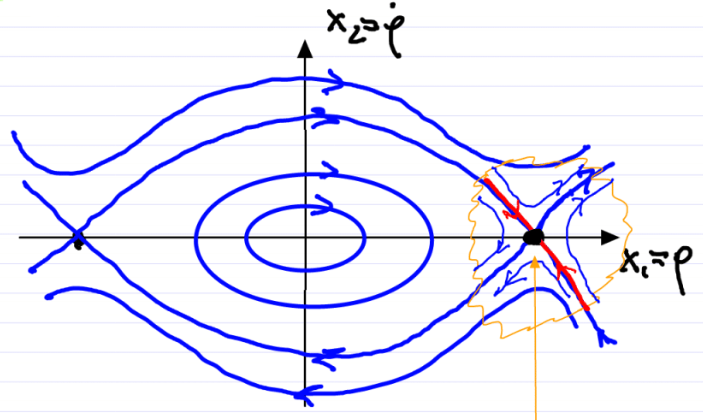
\includegraphics[width=0.6\textwidth]{figures/ch2/7unstable_pendulum.png}
		\caption{The phase portrait around the unstable fixed point of the pendulum, with the stable trajectories (red).}
		\label{fig:convergent_unstable}
	\end{figure}
	
\end{ex}
\newpage
\section{Stability based on linearization}
We would like to derive a more general method to analyze the stability of fixed points, thus we try to simplify our system around the fixed point and discover what this can tell us about the full (unsimplified) system. In the following section we shall always assume that our system is autonomous. We will have the following setup
\begin{align*}
	\dot{ {x}}=f( {x}),\quad f\in \mathcal{C}^1,\quad  {x}=
	\begin{pmatrix}
		x_1\\ \vdots \\ x_n
	\end{pmatrix}\in \mathbb{R}^{n}, \quad 
	{p} = 
\begin{pmatrix}
	p_1 \\ \vdots \\ p_n 
\end{pmatrix}
\in \mathbb{R}^{n}. \numberthis \label{eq:star}
\end{align*}

If $f({p} )={0} $, then ${p} $ is a fixed point. By transforming using ${y} = {x} - {p} $, we have that in the transformed system ${y} = {0} $ is a fixed point. Furthermore, we have that around ${y} = {0} $ the ODE is 
\begin{align}
	\dot{{y} } = f({p} + {y} ) = \underbrace{f({p} )}_{=0} + Df({p} ){y} + o(\| {y} \|) = Df({p} ){y} + o(\| {y} \|).
\end{align}
\begin{remark}[]
	Since we only assumed one continuous derivative for the function $f$ the remainder term in the Taylor approximation is $o(\|y\|)$. The little o notation means that 
	\begin{align}
		\lim_{\|y\| \to 0} \frac{o(\|y\|)}{\|y\|}=0.
	\end{align}
	
\end{remark}

\begin{definition}[Linearized ODE]
	We define the \emph{linearization} of \eqref{eq:star} at the fixed point ${p} $ as 
	\begin{align*}
		\boxed{
		\dot{{y} } = {A} {y}; \quad {y} \in \mathbb{R}^{n},\quad {A} := Df({p} ) \in \mathbb{R}_{n \times n};\quad  Df(p) = 
	\left. \begin{pmatrix}
		\frac{\partial f_1}{\partial x_1} & \ldots & \frac{\partial f_1}{\partial x_n} \\
		\vdots & & \vdots \\
		\frac{\partial f_n}{\partial x_1} & \ldots & \frac{\partial f_n}{\partial x_n}
\end{pmatrix}\right|_{{x} = {p} }.} \numberthis \label{eq:sstar}
	\end{align*}
\end{definition}
Now we would like to study the stability of the fixed point ${y} =0$ in \eqref{eq:sstar}. From this analysis, we want to know the relevance of our results for the full nonlinear system \eqref{eq:star}.

\section{Review of linear dynamical systems}
Recall the setup
\begin{align}
	\dot{{y} } = {A} (t){y}, \quad {y} \in \mathbb{R}^{n}, \quad {A} \in \mathbb{R}^{n \times n}, \quad {A} \in \mathcal{C}^{0}_{t}.
\end{align}
The following facts have already been established
\begin{itemize}
	\item We know that the global existence and uniqueness of solutions is guaranteed. 
	\item The superposition principle holds; namely the linear combination of solutions is also a solution.
	\item There exists a set of $n$ linearly independent solutions: $\varphi_1(t), \ldots, \varphi_n(t) \in \mathbb{R}_{n}$.
	\item The general solution is
		\begin{align}
			y(t) = \sum_{i=1}^{n} c_i \varphi_i(t) =
			\underbrace{\begin{bmatrix}
				\varphi_1(t) & \ldots & \varphi_n(t)
		\end{bmatrix}}_{\Psi(t):  \textrm{ fundamental matrix solution} }
		\underbrace{\begin{bmatrix}
			c_1 \\ \vdots \\ c_n
	\end{bmatrix}}_{c}
	= \Psi(t) {c}; \quad \dot{\Psi} = A(t) \Psi.			
		\end{align}
	\item We have the initial value problem ${y} (t_0) = {y} _0$ which implies
		\begin{align}
			\Psi(t_0) {c} = {y} _0 \implies {y} (t) = \underbrace{\Psi(t) \left[\Psi(t_0)\right]^{-1}}_{\phi(t):= F_{t_0}^{t}}{y} _0 
		\end{align}
		Where we used that the $\varphi_i(t)$ are linearly independent in the last equality. And we have the \emph{normalized fundamental matrix} $\phi(t)$ equal to the flow map, with $\phi(t_0)={I} $.
	\item In the autonomous case $\dot{{x} }= {A} {x} $ solutions can be practically constructed.
	\begin{enumerate} 
		\item \textbf{Explicit Solution} 
		\begin{align}
			\phi(t) = e^{{A} t} := \sum_{j=0}^{\infty } \frac{1}{j!} ({A} t)^{j}
		\end{align}
	With $0! =1$ and ${0} ^{0}= {I} $. We can verify that this is indeed a solution
	\begin{align}
		\dot{\phi}(t) = \sum_{j=1}^{\infty } \frac{1}{(j-1)!} ({A} t)^{j-1}{A} = {A} \sum_{j=0}^{\infty } \frac{1}{j!} ({A} t)^{j} = {A}  e^{{A} t} = {A} \phi(t).
	\end{align}
	Where we used that ${A} $ commutes with its powers in the second equality. We now have that each column of $\phi(t)$ satisfies $\dot{{y} } = {A} {y} $.	
	\begin{remark}[]
		For a scalar ODE $\dot{y}= a(t)y$ for $y \in \mathbb{R}$, the solution is known $y(t) = e^{\int_{t_0}^{t} a(s)ds}y_0$. However, this does not extend to the higher dimensional $\dot{{y} }= {A} (t){y} $. In fact, in general, $\phi(t) = e^{\int_{t_0}^{t} {A} (s)ds}$ is \underline{not} a solution. We can check this
	\begin{align}
		\dot{\phi} = \sum_{j=0}^{\infty } \frac{1}{j!} \frac{d}{dt} \left( \int_{t_0}^{t} {A} (s) ds \right)^{j} = \sum_{j=1}^{\infty } \frac{1}{(j-1)!} \left( \int_{t_0}^{t} {A} (s)ds \right)^{j-1} {A} (t) \neq {A} (t) \phi(t).
	\end{align}
	The nonequality holds as ${A} (t)$ does not generally commute with $\int_{}^{} {A} (s)ds$.
	\end{remark}

\item \textbf{Solution from eigenfunctions} If we have an autonomous system, we can solve the ODE without an infinite series. We have 
	\begin{align*}
		\dot{{y} } = {A} {y} ,\quad {y} \in \mathbb{R}^{n}, \quad {y} (0) = {y}_0. \numberthis \label{eq:onestar}
	\end{align*}
	Substituting $\varphi(t)=e^{\lambda t}{s} $ for $\lambda\in \mathbb{C}$ and ${s} \in \mathbb{C}^{n}$ into \eqref{eq:onestar} yields
\begin{align*}
	\lambda {s} = {A} {s} \implies ( {A} - \lambda {I} ) {s} = 0 \iff \det( {A} - \lambda {I} ) = 0 \numberthis \label{eq:twostar}.
\end{align*}
Therefore $\lambda$ must be an eigenvalue of ${A}$ and ${s} $ must be the corresponding eigenvector. We call $\det({A} - \lambda {I} )$ the \emph{characteristic equation} of ${A} $. Let $\lambda_1, \ldots , \lambda_n$ be the eigenvalues and ${s} _1, \ldots, {s} _n$ be the corresponding eigenvectors. In the case that some eigenvalues are repeated, some of the ${s} _i$ may be generalized eigenvectors. We then have two cases.
\begin{enumerate}
	\item ${A} $ is semisimple, i.e. the eigenvectors are linearly independent (which is always the case if the $\lambda_i$ all have algebraic multiplicity of one). Then we have the solution
		\begin{align}
			{y} (t) = \sum_{i=1}^{n} c_i e^{\lambda_i t}{s} _i = \sum_{j=1}^{n} c_j e^{ (\textrm{Re} \lambda_j) t} e^{i( \textrm{Im} \lambda_j)t} {s} _j.
		\end{align}
	Where we used $\lambda_j =  \textrm{Re} \lambda_j + i  \textrm{Im} \lambda_j$.	
\item ${A} $ is \underline{not} semisimple, i.e. has repeated eigenvalues (but not enough linearly independent eigenvectors). Then we assume that $\lambda_k$ has algebraic multiplicity $a_k > g_k$, where $a_k$ measures the multiplicity of $\lambda_k$ as a root of $\det({A} - \lambda {I} )=0$, and $g_k$ is the number of linearly independent eigenvectors for $\lambda_k$, also called the \emph{geometric muliplicity} of $\lambda_k$. Even in this case, $\lambda _k$ gives rise to $a_k$ linearly independent solutions of the form
	\begin{align}
		\underbrace{{P} _0}_{={s_k} } e^{\lambda _k t},\ {P} _1(t) e^{\lambda _k t}, \ {P}_2(t)e^{\lambda _k t}, \ldots, {P} _{a_{k-1}}(t)e^{\lambda _k t}
	\end{align}
	where ${P} _{j}(t)$ is a vector polynomial of $t$ of order $j$ or less.	
\end{enumerate}

	\end{enumerate}
\end{itemize}

\section{Stability of fixed points in autonomous linear systems}
First we note that we can bound our solution
\begin{align*}
	\| {y} (t) \| = \| \phi(t) {y} _0 \| \leq \underbrace{\| \phi(t) \|}_{ \textrm{Operator norm} } \| {y}_0 \| \leq C e^{\mu t} \| {y} _0 \|. \numberthis \label{eq:1star}
\end{align*}
Where $\mu = \max_j ( \textrm{Re} \lambda_j) + \nu $, with $\nu >0$, as small as needed, provided we increase $C$ appropriately. If ${A} $ is semisimple, then $\nu =0$ can be selected.
\begin{theorem}[Stability of fixed points in linear systems] \label{thm:lin_stab_eigv}
	Given ${y} =0$ a fixed point of the linear system $\dot{{y} } = {A} {y} $ with ${A} \in \mathbb{R}^{n \times n}$ the following statements hold:
	\begin{enumerate}
		\item Assume that $ \textrm{Re} \lambda _j < 0$ for all $j$. Then ${y} =0$ is asymptotically stable.
		\item Assume that $ \textrm{Re} \lambda _j \leq 0$ for all $j$, and for all $\lambda_k$ with $ \textrm{Re} \lambda_k = 0$ we have $a_k = g_k$. Then ${y} =0$ is stable.
		\item Assume there exists a $k$ such that $ \textrm{Re} \lambda _k >0$. Then ${y} =0$ is unstable.
	\end{enumerate}
	These scenarios are illustrated in Fig. \ref{fig:eigv_setup}.
\end{theorem}
\begin{proof}
	\begin{enumerate}
		\item Pick $\varepsilon > 0$, and select $\nu > 0$ small, such that $\mu <0$. Then pick $C> 0$ such that \eqref{eq:1star} holds, and let $\delta = \frac{\varepsilon}{C}$. This implies (since $\| {y} _0\| \leq \delta $) that
			\begin{align}
				\| {y} (t) \| \leq \varepsilon e^{\mu t} \leq \varepsilon,
			\end{align}
		and
		\begin{align}
			\| {y} (t) \| \leq \varepsilon e^{\mu t} \xrightarrow{t \to \infty } 0. 
		\end{align}
	Where the limit holds as $\mu < 0$.	
\item Again choose $\delta = \frac{\varepsilon}{C}$ and note that $\mu  = \max_{j} ( \textrm{Re} \lambda _j) + \nu = 0 + \nu =0$ ($\nu =0$ as $a_k = g_k$). Then stability follows by \eqref{eq:1star}. However, asymptotic stability does not hold, as $\varphi(t) = C e^{i ( \textrm{Im} \lambda _j)t} $ solutions exist.

\item There exists a solution of the form
	\begin{align}
		{	\varphi}(t) = C_k e^{\lambda _k t} {s} _k = C_k e^{( \textrm{Re}  \lambda _k)t} e ^{i ( \textrm{Im} \lambda _k)t}{s} _k.
	\end{align}
In turn this implies
\begin{align}
	\| {\varphi}(t) \| = C_k e^{( \textrm{Re} \lambda_k) t} \| {s} _k \| \xrightarrow{t \to \infty} \infty .
\end{align}

	\end{enumerate}
\end{proof}
\begin{figure}[h!]
	\centering
	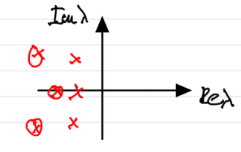
\includegraphics[width=0.3\textwidth]{figures/ch2/8eigv_setup1.png}
	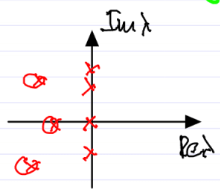
\includegraphics[width=0.3\textwidth]{figures/ch2/9eigv_setup2.png}
	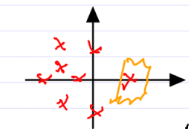
\includegraphics[width=0.3\textwidth]{figures/ch2/10eigv_setup3.png}
	\caption{Eigenvalue arrangements for scenarios (i), (ii), and (iii) (from left to right) in Theorem \ref{thm:lin_stab_eigv}}
	\label{fig:eigv_setup}
\end{figure}

\begin{ex}[Stability analysis of 2 degrees of freedom coupled oscillators]
	Given a rectangular mass $m$ with a spring of stiffness coefficient $k$ attached to each side extending to fixed walls in each cardinal direction. We want to know the stability of the equilibrium where all of the springs are equally extended. This dynamical system is depicted in Fig. \ref{fig:quad_spring}.
\begin{figure}[h!]
	\centering
	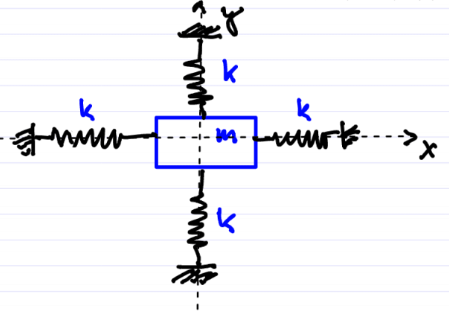
\includegraphics[width= 0.3\textwidth]{figures/ch2/11quad_spring.png}
\caption{Arrangement of coupled oscillators with rectangular mass in the middle.} \label{fig:quad_spring}
\end{figure}
First, note that this is a conservative system, i.e. $E=$ const. Next we transform the coordinates so that the equations of motion can be brought into the form of an ODE for this dynamical system
\begin{align}
	{x} = 
	\begin{pmatrix}
		x \\ \dot{x} \\ y  \\ \dot{y}
	\end{pmatrix}.
\end{align}
Thus we have a 4-dimensional, nonlinear, system of ODEs. We now linearize this at the fixed point $(x,y)= (0,0)$, i.e. $\dot{{x}} = {A} {x} $ with ${x} \in \mathbb{R}^{n}$.

The system exhibits full spatial symmetry in $x$ and $y$, hence the eigenmodes will be the same in the $x$ and $y$ directions. This means we have repeated pairs of purely imaginary eigenvalues for ${A} $:  $\lambda_{1,2}=\lambda_{3,4}= \pm i \omega $. It is clear that scenarios (i) and (iii) of Theorem \ref{thm:lin_stab_eigv} do not apply to the linearized ODE. So we need to check if (ii) applies.

We have that $ \textrm{Re} \lambda _{k}=0$ for $k=1,2,3,4$. Also $a_k=2$ for $k=1,2,3,4$. Now assume $g_k < 2$. Then there would exists solutions of the form $te^{\pm i \omega t}{s}_k$, but this would contradict the conservation of energy, as either the (nonnegative) kinetic energy and/or the (nonnegative) potential energy would grow unbounded. Hence, the total energy could not be conserved. Therefore we know that $g_k = a_k$ and we can apply (ii) to find $x=y=0$ is Lyapunov stable for the linearized system. What does this imply for the nonlinear system?
\end{ex}

\section{Stability of fixed points in nonlinear systems}
Following the previous example, we would like to know what information about the stability of fixed points of nonlinear systems we can derive from the linearized system. The full nonlinear system is
\begin{align*}
	\dot{{x} } = f(x),\quad f({x} _{0}) = {0}, \quad {x} \in \mathbb{R}^{n}, \quad f \in \mathcal{C}^{1}. \numberthis \label{eq:unostar}
\end{align*}
And its linearization at the fixed point ${x} _0$ 
\begin{align*}
	\dot{{y} } = Df({x} _0){y}, \quad y\in \mathbb{R}^{n},\quad Df({x} _0) \in \mathbb{R}^{n\times n}
	\numberthis \label{eq:dosstar}.
\end{align*}
We would like to conclude that the linearized dynamics are qualitatively similar to the nonlinear dynamics. In order to study if this is the case, we have to formalize \emph{similar} mathematically.

\begin{definition}[$\mathcal{C}^k$ equivalence of dynamical systems]
Consider two autonomous dynamical systems:
\begin{enumerate}
	\item
		\begin{align*}
			\dot{{x} }=f({x}),\quad {x} \in \mathbb{R}^{n}, \quad f \in \mathcal{C}^{1};\quad F^{t}: {x_0} \mapsto {x} (t;{x} _0). \numberthis \label{eq:uno}
		\end{align*} 
	\item	
		\begin{align}
			\dot{{x} }=g({x}),\quad {x} \in \mathbb{R}^{n}, \quad g \in \mathcal{C}^{1};\quad G^{t}: {x_0} \mapsto {x} (t;{x} _0).
		\end{align}
\end{enumerate}
The two dynamical systems are \emph{$\mathcal{C}^k$ equivalent}, for $k \in \mathbb{N}$, on an open set $U \subset \mathbb{R}^{n}$, if there exists a $\mathcal{C}^k$ diffeomorphism $h: U \to U$ that maps orbits of (i) into orbits of (ii), while preserving the orientation but not necessarily the exact parameterization of the orbit by time. Specifically for all $x\in U$, any $t _1 \in \mathbb{R}$  there exists a $t_2 \in \mathbb{R}$ such that
\begin{align}
	\boxed{
		h(F^{t_1}({x})) = G^{t_2}(h(x)).
	}
\end{align}
$h:U\to U$ does this for all $x\in U$ in a $\mathcal{C}^{k}$ fashion. This equivalence through a function $h$ is demonstrated in Fig \ref{fig:ck_equiv}.
\begin{figure}[h!]
	\centering
	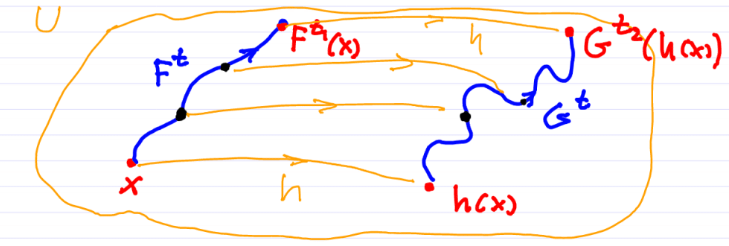
\includegraphics[width=0.7\textwidth]{figures/ch2/12ck_equiv.png}
	\caption{The function $h$ mapping the orbits of the dynamical system describing $F$ into the system describing $G$.}
	\label{fig:ck_equiv}
\end{figure}
\end{definition}
\begin{proposition}[Restrictiveness of smooth equivalence]
	Consider two $\mathcal{C}^{k}$-equivalent dynamical systems for $k>0$ with the right hand sides $f$ and $g$, as in the definitions above. Let $x_0$ be a fixed point of $F$ and $y_0$ a fixed point of $G$ such that these correspond to each other under the $\mathcal{C}^k$ equivalence, i.e. $y_0 = h(x_0)$. The eigenvalues of $Df(x_0)$ must be constant, positive multiples of the eigenvalues of $Dg(y_0)=Dg(h(x_0))$. 	
\end{proposition}
\begin{proof}
	By the $\mathcal{C}^k$ equivalence we have that there exists a $\tau (x,t)$ with $\frac{d \tau}{d t}>0$ such that $h(F^{t}(x)) = G^{\tau(x,t)}(h(x))$. Further assume that $\tau$ is at least continuously differentiable in its arguments. Differentiating the previous equality with respect to  $x$ yields
	\begin{align}
		Dh DF^{t} = \dot{G}^{\tau }\frac{d \tau }{dx} + D G^{\tau} Dh.
	\end{align}
	At a fixed point $x_0$ we have that $\dot{G}^{\tau}(x_0)=g(G^{\tau}(x_0))=0$. This implies that the first term on the right hand side of the differentiated equality is equal to 0. Now denote the linearizations of $f$ and $g$ at the fixed point by $A=Df(x_0)$ and $B=Dg(h(x_0))$ respectively. Then the matrices $e^{A t} $ and $e^{B\tau} $ must be similar matrices, in turn implying that $ At$ and $B\tau(x_0,t)$ must have the same spectrum, i.e.
	\begin{align}
		\frac{\lambda_i(B)}{\lambda_i(A)} = \frac{t}{\tau(x_0,t)} = C =  \textrm{const.}  >0. 
	\end{align}
Therefore the eigenvalues of the linearizations are constant, positive multiples	of each other.
\end{proof}


\begin{definition}[$\mathcal{C}^k$ conjugacy]
	Consider the same two dynamical systems as before. The two dynamical systems are $\mathcal{C}^k$ \emph{conjugate} if there exists a $\mathcal{C}^k$ diffeomorphism $h:U \to U$ that maps orbits of (i) into (ii), while preserving orientation and the parameterization of the orbit by time. Specifically for all $x \in U$ and $t \in \mathbb{R}$ we have
	\begin{align}
		\boxed{
			h(F^{t}(x)) = G^{t}(h(x)).
		}
	\end{align}
\end{definition}

\begin{proposition}[Restrictiveness of smooth conjugacy]
	Consider two $\mathcal{C}^{k}$ conjugate systems, as in the definition above. In addition to the previous proposition, now the linearizations of the two systems will have the same spectra at each fixed point.
\end{proposition}
\begin{proof}
	The $\mathcal{C}^{k}$ conjugacy requires preserving the parameterizations of the orbits, i.e. $\tau(x,t) = t$. Hence, this is just a specification of the previous proof.
\end{proof}


\begin{definition}[Topological equivalence]
	For $k=0$, $\mathcal{C}^{k}$ equivalence is also called \emph{topological equivalence}. In this case, a continuous, invertible deformation takes orbits of one system into the orbits of the other. Under these conditions,  $h:U\to U$ is called a \emph{homeomorhpism}.
\end{definition}

\begin{ex}[Topologically equivalent linear systems for $n=2$]
	To illustrate the meaning of topological equivalence, Fig. \ref{fig:topo_equiv} shows three linear systems ($\dot{{x} } = {Ax}  $ for $x\in \mathbb{R}^2$) which are topologically equivalent.
	\begin{figure}[h!]
		\centering
		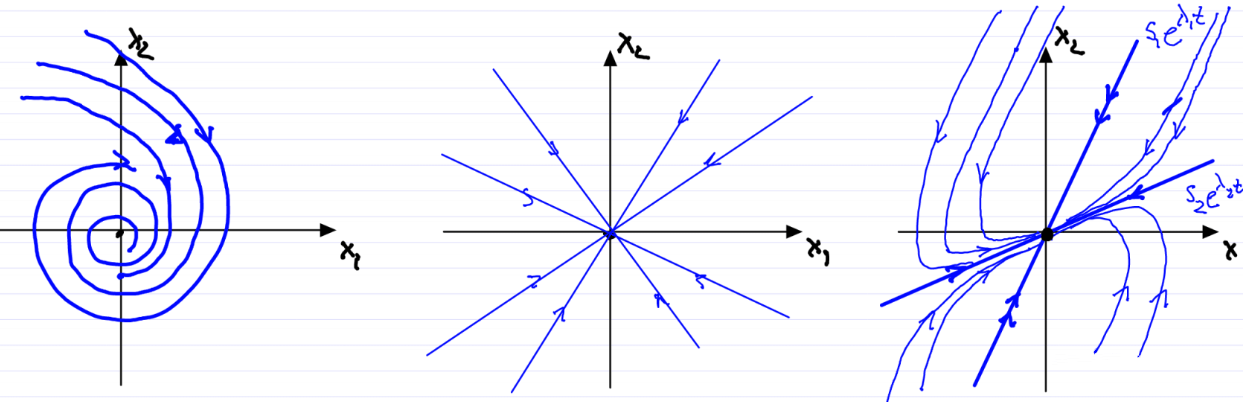
\includegraphics[width=0.9\textwidth]{figures/ch2/13topo_equiv.png}
		\caption{Three topologically equivalent 2-dimensional linear systems. Left: The stable spiral. Middle: The sink. Left: The stable node.}
		\label{fig:topo_equiv}
	\end{figure}

The stable spiral has the eigenvalues $\lambda _{1,2}= \alpha \pm i \beta $ for $\alpha <0$ and $\beta \neq 0$. The sink has the eigenvalues $\lambda_1=\lambda_2<0$. and The stable node has the eigenvalues $\lambda_1 < \lambda_2 < 0$. Note here that the number of eigenvalues $\lambda_i$ with $ \textrm{Re} \lambda_i <0$, $ \textrm{Re} \lambda _i=0$, and $ \textrm{Re} \lambda _i>0$ is the same in all three of these cases, namely for each system the real part of both eigenvalues are less than 0.	
\end{ex}

\begin{remark}[]
	The above systems are not $\mathcal{C}^k$ equivalent or conjugate, as the spectra differ by more than a multiplicative constant.
\end{remark}


\begin{ex}[Topologically inequivalent linear systems for $n=2$]
	As a counter example, we now present three linear systems which are not topologically equivalent. The stable spiral (from before), the unstable spiral, and the saddle. The unstable spiral has the eigenvalues $\lambda _{1,2}= \alpha \pm i \beta $ for $\alpha > 0$ and $\beta \neq 0$ (note the different sign for $\alpha)$. The saddle has the eigenvalues $\lambda _1 < 0 < \lambda_2$. These systems are depicted in Fig \ref{fig:topo_inequiv}.
	\begin{figure}[h!]
		\centering
		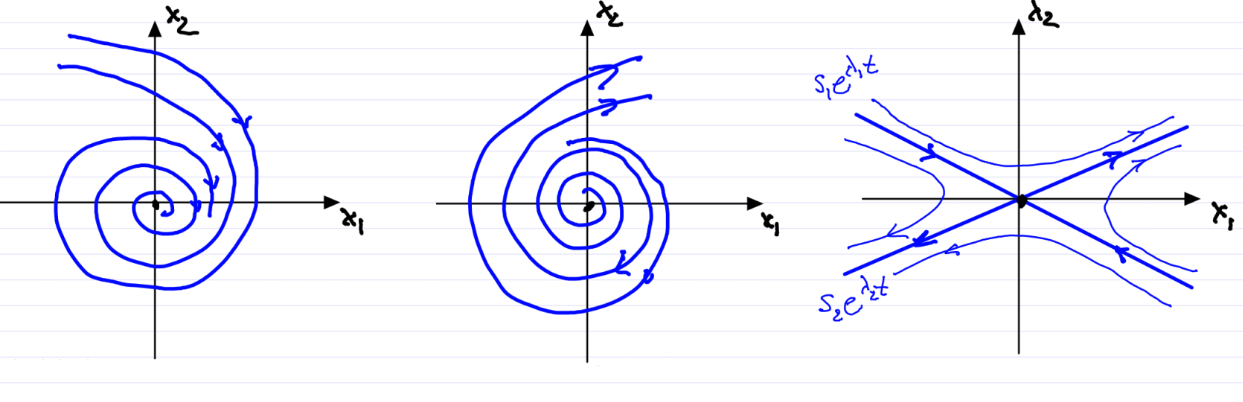
\includegraphics[width=0.9\textwidth]{figures/ch2/14topo_inequiv.png}
		\caption{Three 2-dimensional linear systems which are not topologically equivalent. Left: The stable spiral. Middle: The unstable spiral. Right: The saddle.}
		\label{fig:topo_inequiv}
	\end{figure}

	Note here that the eigenvalue configurations in terms of the number of $\lambda _i$ with real part less than $0$ are different in each case.
Building on the role of the eigenvalue configuration we noted in the previous examples, we introduce the concept of a hyperbolic fixed point.
\end{ex}
\begin{definition}[Hyperbolic fixed point]
	We call the fixed point  ${x} ={x_0} $ a \emph{hyperbolic fixed point} of \eqref{eq:unostar} if each of the eigenvalues $\lambda_i$ of its linearization \eqref{eq:dosstar} satisfy
	\begin{align}
		\boxed{ \textrm{Re} \lambda_i \neq 0.}
	\end{align}
	Geometrically the eigenvalue configuration of a hyperbolic fixed point is shown in Fig. \ref{fig:hyperbol_ex}.
	\begin{figure}[h!]
		\centering
		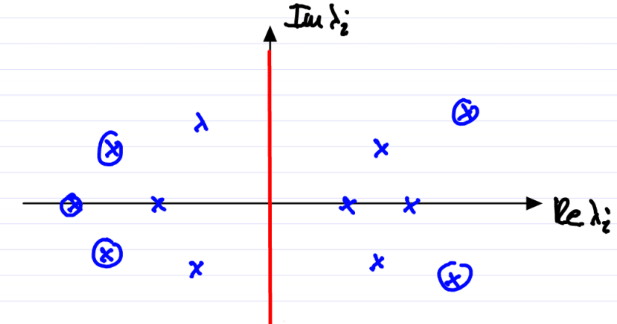
\includegraphics[width=0.6\textwidth]{figures/ch2/15hyperbol_ex}
		\caption{The eigenvalue configuration of a hyperbolic fixed point, i.e. no eigenvalues are on the imaginary axis (red).}
		\label{fig:hyperbol_ex}
	\end{figure}
\end{definition}
	
\begin{proposition}[]
	Under small perturbations to the nonlinear system, the linearized stability type of the hyperbolic fixed point is preserved.
\end{proposition}
Before proving this result, recall the Implicit Function Theorem (without proof).

\begin{theorem}[Implicit Function Theorem ($n+1$ dimensional case)]
	For a function $F:\mathbb{R}^{n+1} \to \mathbb{R}^{n}$ which is $\mathcal{C}^1$, if  $F( {x_0} , y_0 ) = 0$ and the Jacobian $D_{{x} }F({x_0} , y_0 )$ is nonsingular (invertible), then there exists a nearby solution to $F({x} , y )=0 $, for ${x_y} = {x_0}  + \mathcal{O}(|y-y_0|)$. Further ${x_y} $ is as smooth in $y$ as $F({x} ,y)$.
\end{theorem}

\begin{proof}[Proof (Proposition)]
	Add a small perturbation to \eqref{eq:uno} i.e.
\begin{align}
	\dot{{x} } = f({x}) + \varepsilon g({x} );\quad |\varepsilon | \ll 1,\quad f({x} _0) =0.
\end{align}
Now we ask if the perturbed system has a fixed point ${x} _{\varepsilon}$ near ${x} _0$. We frame this in terms of the implicit function theorem
\begin{align}
	F({x} ,\varepsilon) = f({x} ) + \varepsilon g({x} ) \stackrel{?}{=} 0;\quad F({x}_0, 0) = 0;\quad {x} \in \mathbb{R}^{n}, \quad F:\mathbb{R}^{n+1} \to \mathbb{R}^{1}.
\end{align}
We check that $D_{{x} }F({x_0} ,0) $ is nonsingular exactly when $Df({x_0)} $ is; this is fulfilled as we have no zero eigenvalues. The linearization at the perturbed fixed point takes the form
\begin{align}
	\dot{{y} } = D \left. \left[ f({x} ) + \varepsilon g({x} ) \right]\right|_{{x} = {x_\varepsilon} }{y} = \left[ Df({x_0}  + \mathcal{O}(\varepsilon)) + \varepsilon Dg({x_0} + \mathcal{O}(\varepsilon)) \right] {y} 
		=\underbrace{ \left[ Df({x_0})+ \mathcal{O}(\varepsilon) \right]}_{={A_{\varepsilon}} }{y}.
\end{align}
In the last equality we used the Taylor expansion in $\varepsilon$. We have that the roots of $\det({A_{\varepsilon}}-\lambda {I} ) = 0 $ depend continuously on the parameter $\varepsilon$. These roots correspond to the eigenvalues of $A_{\varepsilon}$. Therefore, the roots stay within an $\mathcal{O}(\varepsilon)$ neighborhood of the eigenvalues of $Df({x_0} )$ (see Fig. \ref{fig:eps_ball_eigv}). Hence we have that the eigenvalue configuration is unchanged for small enough $\varepsilon$.
\begin{figure}[h!]
	\centering
	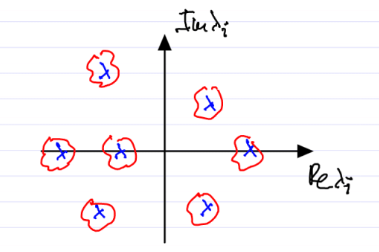
\includegraphics[width=0.5\textwidth]{figures/ch2/16eps_ball_eigv.png}
	\caption{The eigenvalue configuration the $\mathcal{O}(\varepsilon)$ neighborhood (red) drawn around each eigenvalue (blue).}
	\label{fig:eps_ball_eigv}
\end{figure}
\end{proof}
\begin{remark}[]
	In the above proof, not only does the hyperbolicity of fixed points remain preserved, but also the stability type.
\end{remark}
Meanwhile, for nonhyperbolic fixed points, this is not the case, and the smallest perturbation may change their stability type. This is due to the fact, that no matter how small the scale of the perturbation ($\varepsilon$) the $\mathcal{O}(\varepsilon)$ ball around eigenvalues on the imaginary axis will always intersect with $\mathbb{C}- \{  \textrm{Im}\lambda_i =0 \}$ (i.e. points which are not on the imaginary axis).

Now we would like to connect the preservation of stability type under nonlinear perturbation to analyzing the stability type of fixed points of nonlinear dynamical systems based on their linearization. 
\begin{theorem}[Hartman-Grobman]
	If the fixed point ${x_0} $ of the nonlinear system \eqref{eq:unostar} is hyperbolic, then the linearization \eqref{eq:dosstar} is topologically equivalent to the nonlinear system in a neighborhood of ${x_0} $. 

	\textbf{Consequence:} For hyperbolic fixed points, linearization predicts the correct stability type \underline{and} orbit geometry near ${x_0} $. 
\end{theorem}
Now we would like to apply this to the pendulum to systematically derive the stability type of its fixed points.
\begin{ex}[Stability analysis of the pendulum via Hartman-Grobman]
	Recall the transformed ODE for the pendulum
	\begin{align}
		\dot{x}=f(x)=
		\begin{dcases}
		\dot{x}_{1} = x_2 \\ \dot{x}_2 = -\sin(x_1)	
		\end{dcases}
		;\quad {x}  = 
		\begin{pmatrix}
			x_1 \\ x_2
		\end{pmatrix}
		.
	\end{align}
	We have two fixed points ${p} =(\pi ,0)$ and ${q} = (0,0)$. First we analyze the stability of the fixed point ${p} $. The differential of $f$ at a point $a$ is
\begin{align}
	Df(a) =  
		\begin{pmatrix}
			0 & 1 \\
			-\cos(a_1) & 0
		\end{pmatrix}.
\end{align}
	Start by linearizing at ${p} $ 
	\begin{align}
		\dot{{y} } = {Ay};\quad {A}  = Df({p} ) = 
		\begin{pmatrix}
			0 & 1 \\
			- \cos(x_1) & 0
		\end{pmatrix}_{{x} = {p} } =
		\begin{pmatrix}
			0 & 1 \\ 1 & 0
		\end{pmatrix}.
	\end{align}
	Now we have to check if ${p} $ is hyperbolic
	\begin{align}
		\det({A} - \lambda {I} ) = \lambda^2 -1 = 0 \implies \lambda_{1,2} = \pm 1;\ {s_1} =
		\begin{pmatrix}
			1 \\ 1
		\end{pmatrix}
		,\ {s_2} =
		\begin{pmatrix}
			-1 \\ 1
		\end{pmatrix}.
	\end{align}
	Neither of the eigenvalues lie on the imaginary axis, so $p$ is hyperbolic. This allows us to move between the nonlinear and linearized system for the stability analysis without compromising our results. We find the linearized dynamics to be
	\begin{align}
		{y} (t) = C_1 e^{t} {s_1}  + C_2 e^{-t}{s_2}.
	\end{align}
	Using the initial conditions $y_0$ the trajectory can be expressed as
	\begin{align}
		y(t) =  F^{t}{y_0}, 
	\end{align}
	where $F^{t}$ is the normalized fundamental matrix solution. We can now fully describe the phase portrait of the linearization. The \emph{stable subspace} $E^{S}$ is $ \textrm{span} \{{s_2} \} = \{{y_0} :\ F^{t}{y_0} \xrightarrow{t \to \infty} 0 \} $. The unstable subspace $E^{U}$ is $ \textrm{span} \{{s_1}\} = \{{y_0} : \ F^{t}{y_0} \xrightarrow{t \to - \infty }0\} $. The phase portrait near the fixed point $p$ is illustrated in Fig. \ref{fig:pend_phase_p}
\begin{figure}[h!]
	\centering
	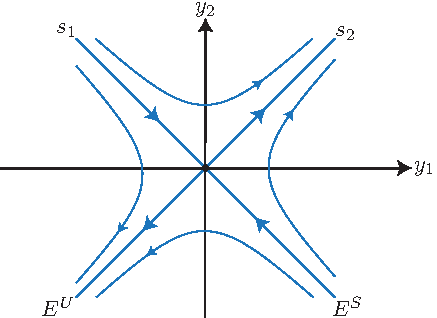
\includegraphics[width=0.4\textwidth]{figures/ch2/17pend_phase_p}
	\caption{The phase portrait of the linearized pendulum in a neighborhood around ${p} $.}
	\label{fig:pend_phase_p}
\end{figure}

The nonlinear phase portrait is topologically equivalent to the linear one. Further we can define the stable and unstable manifolds of ${p} $ for the nonlinear system. We designate $F^{t}(\cdot)$ to be the flow map for the nonlinear system after this point.
The \emph{stable manifold} of ${p} $ is 
\begin{align}
	\boxed{
	W^{S} = \{ {x_0} :\ F^{t}({x_0} ) \xrightarrow{t \to \infty}{p} \}.
}
\end{align}
and the \emph{unstable manifold} of ${p} $
\begin{align}
	\boxed{
	W^{U}=\{{x_0} :\ F^{t}({x_0} ) \xrightarrow{t \to - \infty}{p}\}.
}
\end{align}
Both of these are $\mathcal{C}^{0}$ curves through ${p}$ and their existence follows from the Hartman-Grobman theorem. These manifolds are shown in the nonlinear phase portrait around ${p} $ in Fig. \ref{fig:nonlin_pend_phase_p}. 
\begin{figure}[h!]
	\centering
	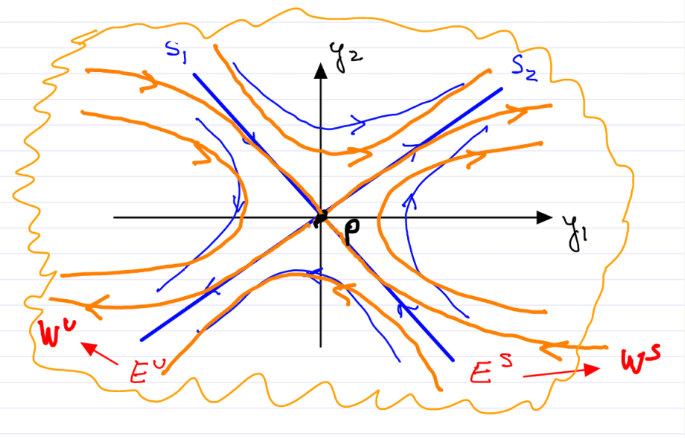
\includegraphics[width=0.6\textwidth]{figures/ch2/18nonlin_pend_phase_p.png}
	\caption{The phase portrait of the pendulum on a neighborhood around ${p} $ with the stable and unstable manifolds of the nonlinear system as well as the stable and unstable spaces of the linearization.}
	\label{fig:nonlin_pend_phase_p}
\end{figure}

Next we analyze the stability of the fixed point $q$. Once again, our first step is to linearize
\begin{align}
	\dot{y} = Ay, \quad A = Df(q) = 
	\begin{pmatrix}
		0 & 1 \\ -1 & 0
	\end{pmatrix}
	;\quad \det (A- \lambda I) = 0.
\end{align}
From here, we see that the determinant is equal $\lambda^2 + 1 = 0$, yielding the roots $\lambda_{1,2}= \pm i$, i.e. the fixed point is \underline{not} hyperbolic. Thus the linearized dynamics is inconclusive for the nonlinear system. In this particular case, $q$ turns out to be stable by the definition of Lyapunov stability. Later we will use another approach to show this directly.
\end{ex}

In the last example, the importance of hyperbolicity was not accentuated, as the latter fixed point had the same stability type in the linearized system as in the full system. This leads us to question if there are cases where the stability type between the linear and nonlinear systems is not preserved.

\begin{ex}[Criticality of hyperbolicity in Hartman-Grobman]
	Let the dynamical system be
	\begin{align}
		\dot{x} = ax^3,\quad x\in\mathbb{R},\quad a \neq 0.
	\end{align}
	This system has a fixed point at $x=0$, linearizing here gives
	\begin{align}
		A = \left. 3ax^2 \right|_{x=0} = 0 \implies \dot{y}= 0y = 0.
	\end{align}
	We have a single root $\lambda_1 = 0$, hence $x=0$ is a nonhyperbolic fixed point. Disregarding this fact, we may be inclined to conclude that $x=0$ is a stable fixed point, since $y=0$ is trivially a fixed point of the linearization $\dot{y}=0$. This is not the case, as we can see by analyzing the full nonlinear dynamics for $a>0$ as in Fig. \ref{fig:hyperbol_counter_ex}, where we observe that $x=0$ is an unstable fixed point.
\begin{figure}[h!]
	\centering
	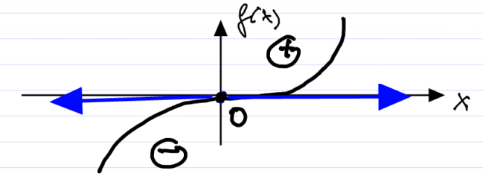
\includegraphics[width=0.5\textwidth]{figures/ch2/19hyperbol_counter_ex.png}
	\caption{Nonlinear dynamics for the dynamical system $\dot{x}= ax^3$ with $a>0$.}
	\label{fig:hyperbol_counter_ex}
\end{figure}
\end{ex}

Now that we have understood how to use the Hartman-Grobman theorem, we would like to to be able to definitely conclude the stability type of a fixed point, once we have the linearization. To achieve this, we require a sufficient and necessary criterion for all of the eigenvalues of the linearized system to be left of the imaginary axis, i.e. $ \textrm{Re} \lambda_i < 0$ for all $i$.

\begin{theorem}[Routh-Hurwitz]
Consider the polynomial
\begin{align}
	a_n \lambda^{n} + a_{n-1} \lambda ^{n-1} + \ldots + a_{1} \lambda + a_0 = 0.
\end{align}
Without loss of generality assume $a_0 > 0$, if $a_0 <0$ then multiply by $-1$ and if $a_0=0$ then $\lambda =0$ is a root and therefore we cannot have asymptotic stability. Next, define the following series of subdeterminants
\begin{align}
	D_0 = a_0,\ D_1 =a_1,\ D_2 =
	\begin{vmatrix}
		a_1 & a_0 \\
		a_3 & a_2
	\end{vmatrix}
	,\ D_3 = 
	\begin{vmatrix}
		a_1 & a_0 & 0 \\
		a_3 & a_2 & a_1 \\
		a_5 & a_4 & a_3
	\end{vmatrix}
	,\ldots,\ D_n =
	\begin{vmatrix}
		a_1 & a_0 & 0 & \ldots & 0 \\
		a_3 & a_2 & a_1 & \ldots & 0 \\
		\vdots & & & & \vdots \\
		0 & \ldots &  a_n & a_{n-1} & a_{n-2}\\
		0 &  \ldots  & & 0  & a_n
	\end{vmatrix}
\end{align}
Then we have that if and only if for all $i$ $D_i >0$ then $ \textrm{Re} \lambda_i <0$ for all $i$.

A weaker neccesary condition is that if for all $i$ $ \textrm{Re} \lambda _i<0$ then $a_i >0$ for all $i$. Therefore if there exists an $a_k<0$, we know immediately that the fixed point cannot be asymptotically stable as not all of the $ \textrm{Re} \lambda _i $ can be strictly negative.
\end{theorem}
\begin{remark}[]
For a given $i$ we construct the matrix used for calculating $D_i$ as follows: write the elements $a_1,\ldots,a_i$ along the diagonal, then in each row $k$ write the $a_j$ in descending index order such that $a_k$ aligns with the placement inherited from us writing along the diagonal. The leftover spaces are filled with zeros. 
\end{remark}

\begin{remark}[]
	Adolf Hurwitz discovered this criterion independently of Edward Routh in 1895 while holding a chair at the ETH.
\end{remark}

\begin{ex}[Applying the Routh-Hurwitz criterion]
	Given the polynomial
	\begin{align}
		a_3 \lambda ^3 + a_2 \lambda^2 + a_1 \lambda + a_0 = 0.
	\end{align}
	The Routh-Hurwitz criterion is
	\begin{align}
	D_0 = a_0 > 0;\ D_1 = a_1 >0;\ D_2 = a_1 a_2 - a_0 a_3>0;\ D_3 = a_3 D_2 >0.	
	\end{align}
	Therefore 
	\begin{align}
		\boxed{
			a_0> 0,\ a_1 > 0,\ a_1a_2 - a_0a_3 > 0,\ a_3 > 0
		}
	\end{align}
	forms a sufficient and necessary condition for asymptotic stability ($a_i >0$ follows from here) for $n=3$.
\end{ex}

A more refined linearization result comes from Sternberg's Theorem \cite{Chicone}.
\begin{theorem}[Sternberg]
Assume the following
\begin{enumerate}
	\item The fixed point is asymptotically stable, i.e. $ \textrm{Re} \lambda _j<0$ for all $j=1,\ldots,n$ (this also implies hyperbolicity);
	\item $f\in \mathcal{C}^{r}$ for $r\in \mathbb{N}\cup \{\infty \}$ and $r>\frac{\max_{j}| \textrm{Re} \lambda _j|}{\min_{j}| \textrm{Im} \lambda _j|}$;
	\item The system is nonresonant, i.e. 
		\begin{align}
			\sum_{j=1}^{n}m_j \lambda _j \neq \lambda_k,\ \forall k
		\end{align}
	for any sequence $m_j \in \mathbb{N}$ with $\sum_{j=1}^{n} m_j \geq 2$.
	
\end{enumerate}
Then the following holds: $\dot{x}=f(x)$ with $f(0)=0$ is locally $\mathcal{C}^{r}$ conjugate to its linear part $\dot{y}=Ay$ for $A= Df(0)$.
\end{theorem}


\begin{ex}[Watt's centrifugal governor for steam engines]
	Now we put together everything built until now in the example of Watt's centrifugal governor for steam engines. Originally this system was used in mills in the 1700's, then it was adapted by Watt to the steam engine in 1788. This adaptation has been credited as a major factor in the industrial revolution, and is a first example of feedback control. The system is outlined in Fig. \ref{fig:governor}.
\begin{figure}[h!]
	\centering
	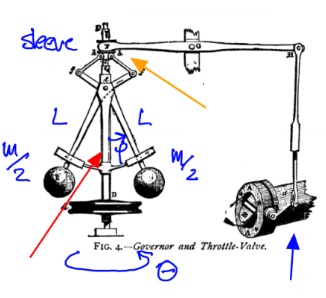
\includegraphics[width=0.34\textwidth]{figures/ch2/20governor.png}
	\caption{Schematic for Watt's centrifugal governor. The yellow arrow points towards a damper on the rotation about the spindle (red arrow). On the right the blue arrow designates a steam engine cylinder.}
	\label{fig:governor}
\end{figure}
The two masses (of mass $\frac{m}{2}$) rotate counter clockwise, and their position in radians is given by $\theta$, with their rotational velocity $\dot{\theta}$. The masses are attached by a rod of length $L$ and their deflection from the vertical position is measured by $\varphi$. Smaller $\dot{\theta}$ allowed for an increase in steam supply.

Following changes in the design, the systems suddenly became unstable. To address this Vyshnegradsky studied the root cause in 1877. We first derive the equation of motion. For the governor we use the equation of motion for a rotating hoop (with viscous damping coefficient $b$).
\begin{align}
	mL^2 \ddot{\varphi} + +bL^2 \dot{\varphi} +mL^2\left( \frac{g}{L} - \dot{\theta}^2 \cos(\varphi) \right) \sin(\varphi) = 0;\quad b>0.
\end{align}
Next, let $\omega $ denote the angular velocity of the steam engine, i.e. with the gear ratio $n$ we have $\dot{\theta} = n \omega$. Then we find
\begin{align}
	m \ddot{\varphi} = -b \dot{\varphi} - m \left( \frac{g}{L} - n^2 w^2 \cos(\varphi) \right) \sin(\varphi).
\end{align}
Now we derive the equation of motion for the steam engine. Denote the moment of inertia for the engine by $J$, the driving torque from the steam as $P_1$ and the constant load $P$, we obtain
\begin{align}
	J \dot{\omega } = P_1 - P.
\end{align}
In this case we have $P_1 = P^{*} + k\left( \cos(\varphi) - \cos(\varphi^{*}) \right)$ for the desired operation angle $\varphi^{*}$, the gain $k$, and $P*$ the value of $P$ at $\varphi^{*}$. Putting this together yields
\begin{align}
	J \dot{\omega } = k \cos(\varphi) - P_0;\quad P_0 = P - P^{*} + k \cos(\varphi^{*}).
\end{align}
Let $\dot{\varphi} = \Psi$ to transform into a three-dimensional set of equations (ODE)
\begin{align}
	\begin{dcases}
		\dot{\varphi} = \Psi \\
		\dot{\Psi} = -\frac{b}{m} \Psi - \left( \frac{g}{L} - n^2 \omega^2 \cos(\varphi) \right) \sin (\varphi) \\
		\dot{\omega } = \frac{k}{J}\cos(\varphi) - \frac{P_0}{J}.
	\end{dcases};
	\quad x =
	\begin{pmatrix}
		\varphi \\ \Psi \\ \omega 
	\end{pmatrix}
	.
\end{align}
Then our operation point is the fixed point $x_0$ of this system
\begin{align}
	f(x_0) = 0 \implies \Psi_0 = 0;\ \omega_0^2 = \frac{g}{Ln^2 \cos(\varphi_0)};\ \cos(\varphi_0) = \frac{P_0}{k}.
\end{align}
If $\sin(\varphi_0)=0$, we have an unphysical state and ignore this case. For simplification set $L=1$, this could be formally achieved by nondimensionalizing the length $L$. Now we linearize at the fixed point $x_0$ 
\begin{align}
	\dot{y} = Ay; \quad A = Df(x_0) =
	\begin{pmatrix}
		0 & 1 & 0 \\
		n^2 \omega^2 \cos(2\varphi_0) -g\cos(\varphi_0) & -\frac{b}{m} & n^2 \omega _0 \sin(2\varphi_0) \\
		-\frac{k}{J}\sin(\varphi_0) & 0 & 0
	\end{pmatrix}
.	
\end{align}
With this we obtain the characteristic equation $\det(A - \lambda I )= 0$ 
\begin{align}
	\underbrace{1}_{a_3} \lambda^3 + \underbrace{\frac{b}{m}}_{a_2}\lambda ^2 + \underbrace{ {g}\frac{\sin^2(\varphi_0)}{\cos(\varphi_0)}}_{a_1} \lambda + \underbrace{ {g} \frac{2k \sin^2 (\varphi_0)}{J \omega_0}}_{a_0} = 0.
\end{align}
Now check the Routh-Hurwitz criterion for asymptotic stability:
\begin{enumerate}
	\item The necessary condition for $ \textrm{Re} \lambda _k<0$ for all $k$: $a_j> 0$ for all $ j$ is fulfilled.
	\item Next we check the subdeterminants
		\begin{subequations}
\begin{align}
	D_0 &= a_0 = {g} \frac{2k \sin^2 (\varphi_0)}{J \omega_0}>0;\quad \\ 
	D_1 &= a_1 = {g}\frac{\sin^2 (\varphi_0)}{\cos(\varphi_0)} >0; \\
	D_2 &= 
	\begin{vmatrix}
		a_1 & a_0 \\
		a_3 & a_2
	\end{vmatrix}
	= a_1a_2 - a_0a_3 = g\frac{b}{m}\frac{\sin^2(\varphi_0)}{\cos(\varphi_0)} - g\frac{2k \sin^2(\varphi_0)}{J \omega_0} >0;\\
	D_3 &> 0 \iff D_2 >0  \textrm{ and } a_3=1>0.
\end{align}
		\end{subequations}
The only actual condition for $x_0$ to be asymptotically stable is $D_2 >0$ 
\begin{align}
	\frac{bJ}{m} > \frac{2 P_0}{\omega_0}.
\end{align}
From the equation for the fixed points we know 
\begin{subequations}
\begin{align}
	P_0 \omega_0^2 = \frac{gk}{Ln^2} =  \textrm{const.} \numberthis \label{eq:watt1}\\
	\omega_0^2 + 2P_0 \omega_0 \frac{d \omega_0}{d P_0} = 0.
\end{align}
\end{subequations}
From the first equation, we realize that we must write $\omega_0 = \omega_0(P_0)$. To obtain the second equation, we derive the first equation \eqref{eq:watt1} with respect to $P_0$. Therefore we find 
\begin{align}
	\frac{d \omega_0}{d P_0} = - \frac{\omega_0}{2P_0}.
\end{align}

\end{enumerate}
Next, define the \emph{non-uniformity of performance}
\begin{align}
	\nu = \left| \frac{d \omega_0}{d P_0} \right| = \frac{\omega_0}{2P_0}.
\end{align}
Then our criterion for asymptotic stability becomes
\begin{align}
\frac{bJ}{m}\nu > 1.	
\end{align}
To conclude, the following have harmful effects of stability
\begin{itemize}
	\item Bigger engines which increase $m$ 
	\item Better machining of surfaces decreasing $b$ 
	\item Increased operating speed decreasing $J$ 
	\item Versatility in operation decreasing $\nu $.
\end{itemize}
These have the effect of pushing the eigenvalues to the right in the complex plane (towards the imaginary axis) as is illustrated in Fig \ref{fig:watt_eigv}.
\begin{figure}[h!]
	\centering
	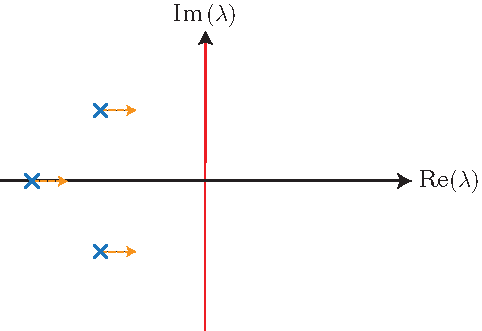
\includegraphics[width=0.4\textwidth]{figures/ch2/21watt_eigv}
	\caption{Change in the eigenvalue configuration as small modification are made to the Watt engine governor.}
	\label{fig:watt_eigv}
\end{figure}
\end{ex}
\newpage

 \section{Data-driven linear modeling of dynamical systems}
 Given are $m+1$ vectors of $n$-dimensional observables $x_0,\ldots,x_m \in \mathbb{R}^{n}$ observed at $\Delta t$ intervals. An example of such data would be many different trajectories or snapshots of a single trajectory. Typically $m \gg 1$, i.e. there are a high number of observations.

 Our objective is to find the best fitting linear dynamical system
 \begin{align}
 	\dot{x}=Ax;\quad x \in \mathbb{R}^{n};\quad A \in \mathbb{R}^{n\times n}.
 \end{align}
Since the data is given as discrete observations, this is equivalent to seeking the best $B=e^{A\Delta t}$ such that $x_{k+1} =Bx_k$ for $k=1,\ldots, m-1$. To solve this we synthesize the data into matrices
\begin{align}
	X = 
	\begin{bmatrix}
		x_0 \ldots x_{m-1}
	\end{bmatrix}
	\in \mathbb{R}^{n\times m}
;\quad
	Y = 
	\begin{bmatrix}
		x_1 \ldots x_{m}
	\end{bmatrix}
	\in \mathbb{R}^{n\times m}.
\end{align}
Notice that the matrix $Y$ is shifted forward compared to the matrix $X$ by $\Delta t$. Next, we solve for  a matrix $B$ that minimizes the distance between $Y $ and $BX$. That is, we find
\begin{align}
	B_{*} =  \underset{B \in \mathbb{R}^{n\times n}}{\textrm{argmin }} g(B);\quad g(B) = \| Y - BX \|^{2} \numberthis \label{eq3:star},
\end{align}
where the matrix norm is the Frobenius norm. We denote the components of $B$ by $b_{ij}$, the components of $Y$ by $y_{ij}$, and the components of $X$ by $x_{ij}$. Note that
\begin{subequations}
\begin{align}
	\frac{\partial g}{\partial b_{ij}} &= \frac{\partial}{\partial b_{ij}} \sum_{l,m,p}^{} \left(y_{lm} - b_{lp}x_{pm}\right)^{2} 
	= -2 \sum_{l,m,p}^{} \left( y_{lm}-b_{lp}x_{pm}\right) \delta_{il}\delta_{jp}x_{pm} \\
					   &= -2\sum_{m,p}^{} \left(y_{im}-b_{ip}x_{pm}\right) x_{jm} 
					   = 2\left(YX^{T} - BX X^{T}\right).
\end{align}
\end{subequations}
In the third equality we have used the properties of the Kronecker-delta $\delta_{ij}$. Therefore we must have that $D_{B}g = -2\left(YX^{T} - BXX^{T}\right)=0$, so we must solve the linear system of equations
\begin{align}
	BXX^{T} = YX^{T}\in \mathbb{R}^{n \times n}.
\end{align}
In the case $n>m$, the matrix $X^{T}$ has more columns than rows, thus $X^{T}$ is singular. Hence $XX^{T}$ has a nonempty kernel and is therefore not invertible. For $n<m$ this is not necessarily the case. For a solution, we can use the pseudo inverse $(XX^{T})^{\dagger}$, the superscript here is called \emph{dagger}.

Recall that if $A \in \mathbb{R}^{n\times n}$ is invertible then $A^{-1} = A^{\dagger}$. If $A$ is not invertible, then calculate the singular value decomposition of $A = U \Sigma V^{T}$ for $U,V \in  \textrm{SO} (n)$ and $\Sigma$ a diagonal matrix. The entries of $\Sigma$ are the strictly positive singular values. The columns of $U$ and $V$ are the left and right singular vectors. We then define the pseudo inverse as
\begin{align}
	A^{\dagger} = V \Sigma^{\dagger} U^{T};\quad \Sigma_{ij}^{\dagger} = 
	\begin{cases}
		\frac{1}{\Sigma_{ij}} & \Sigma_{ij} \neq 0\\
		0 & \Sigma_{ij}=0.
	\end{cases}
\end{align}

This means that for $Ax=b$, the best solution in a least squares sense is given by $x= A^{\dagger}b$. In our case, the solution to \ref{eq3:star} is 
\begin{align}
	B = \left(Y X^{T}\right) \left( XX^{T}\right)^{\dagger}.
\end{align}
This procedure is called \emph{dynamic mode decomposition} (DMD) \cite{Schmid2010, Kutz2016}. The eigenvectors of $B$ are called \emph{DMD modes} and the normalized exponents of those corresponding eigenvalues are called \emph{DMD eigenvalues}.

The procedure has been extended in \emph{extended DMD}, where DMD was performed on functions of the observables (typically polynomials) \cite{Williams2015}. This effectively tries to construct the linearization from data. Note here that none of these procedures can describe intrinsically nonlinear phenomena (i.e. those with coexisting isolated compact invariant sets). 

\begin{remark}[]
The numerical cost of (pseudo)inverting the $n \times n$ matrix, $XX^T$, can be reduced when $n\gg m$.
\begin{enumerate}
\item We can calculate the singular value decomposition of the data matrix $X$ instead. 
\item By keeping only the leading $r$ singular values in this decomposition, we obtain a reduced (rank-$r$) approximation of the matrix $B\in \mathbb{R}^{n \times n}$ as follows. Denote the singular value decomposition by $X = U\Sigma V^T$.  This also means that $(XX^T) = U\Sigma^2 U^T$, i. e. we get the same $U$ as before, but from an SVD of an $n\times m$ matrix, which is much less demanding numerically.

 With the leading $r$ singular vectors and singular values $\sigma$, $X$ can be written as
\begin{equation}
X \approx U_r \Sigma_r V_r^T = \sum_{i=1}^r \sigma_i u_i v_i^T, \qquad U = [u_1, ..., u_n]\quad V = [v_1, ..., v_m].
\end{equation}
\item The matrix $B$ can be approximately written as 
	\begin{subequations}
\begin{align}
B &= YX^T(XX^T)^\dagger \\
& \approx YV_r\Sigma_rU_r^TU_r(\Sigma_r^2)^\dagger U_r^T \\
&= YV_r\Sigma_r^\dagger U_r^T = Y(X_r)^\dagger.
\end{align}\end{subequations}
We denote the truncated approximation of $B$ as $B_r = Y (X_r)^\dagger.$
\end{enumerate}
\end{remark}
	
	
\section{Lyapunov's direct (second) method for stability}
Stability analysis via linearization is not perfect. For nonhyperbolic fixed points, the results obtained are inconclusive, and this case turns out to be somewhat common for conservative systems. Furthermore, linearization does not give any insight into the size of the domain of stability. Hence, a method for determining stability type without relying on linearization would be desirable. This is given to us by Lyapunov's direct method.

\begin{theorem}[] \label{thm:direct}
	Consider
	\begin{align}
		\dot{x} = f(x), \quad f\in \mathcal{C}^1,\quad x \in \mathbb{R}^{n};\quad f(x_0) = 0.
	\end{align}
	Assume that there exists a function $V:U \to \mathbb{R}$ with $V\in \mathcal{C}^1(U)$ for an open set $U \subset \mathbb{R}^{n}$ and $x_0 \in U$ which fulfills the following
	\begin{enumerate}
		\item $V$ is positive definite in a neighborhood of $x_0$, i.e.
			\begin{align}
				V(x_0)=0;\quad V(x)>0,\ x\in U-\{ x_0 \}.
			\end{align}
		\item $\dot{V}$ is negative semidefinite in the same neighborhood, i.e.
			\begin{align}
				\dot{V} =\frac{d}{dt}V(x(t))= 
				\langle DV(x(t)), \dot{x}(t) \rangle =
				\langle DV(x(t)), f(x(t)) \rangle \leq 0,\ x\in U.
			\end{align}
	\end{enumerate}
	Then $x=x_0$ is Lyapunov stable (cf. Def. \ref{def:stable}). $V$ is called a Lyapunov function. The hypotheses are illustrated in Fig. \ref{fig:lyap_thm_assumptions}.	
\end{theorem}
\begin{figure}[h!]
	\centering
	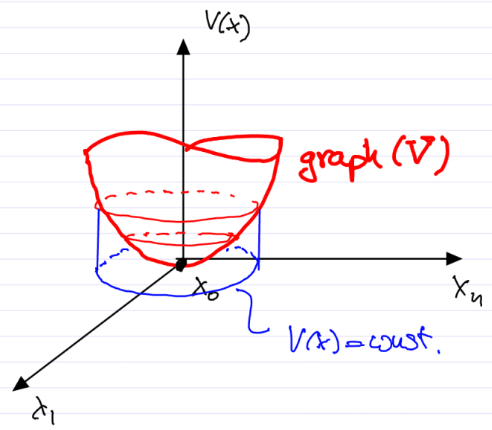
\includegraphics[width=0.4\textwidth]{figures/ch2/23lyap_thm_assumptions1.png}
	\hspace{0.05\textwidth}
	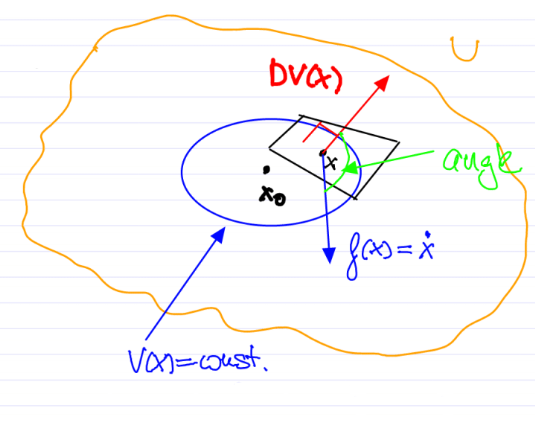
\includegraphics[width=0.4\textwidth]{figures/ch2/23lyap_thm_assumptions2.png}
	\caption{Geometric interpretation of hypotheses of Lyapunov's direct method. Left depicts hypothesis (i) and right hypothesis (ii). The angle between $DV(x)$ and $f(x)$ is at least $\frac{\pi }{2}$. In each image the blue $V(x)=$const. is a level surface diffeomorphic to $S^{n-1}$.}
	\label{fig:lyap_thm_assumptions}
\end{figure}

	\begin{remark}[]
		To denote the boundary of a set $A$ we write $\partial A$.
	\end{remark}
\begin{proof}
	
	First choose $\varepsilon > 0$ and define $\alpha(\varepsilon)= \min_{x\in \partial B_\varepsilon(x_0)} V(x) > 0$. Note that $\alpha(\varepsilon)$ is well defined as $V\in \mathcal{C}^{0}(U)$ and $\partial B_{\varepsilon}(x)$ is compact and spherical for small enough $\varepsilon$. There exists an $x^{*} \in \partial B_{\varepsilon}(x)$ with $V(x^{*}) = \alpha(\varepsilon) \leq V(x)$ for all $x\in \partial B_{\varepsilon}(x_0)$. Next, define $U_{\varepsilon}= \{ x\in B_{\varepsilon}(x_0):\ V(x) < \alpha(\varepsilon)  \ $. Notice that $x_0 \in U_{\varepsilon}$ because $V(x_0) =0$ and $V(x)\geq 0$ on $U$. Further $U_{\varepsilon}$ is open due to the continuity of $V$. We have that  $U_{\varepsilon} \cap \partial B_{\varepsilon}(x_ 0) $ is empty by definintion, noting that for all $x\in \partial B_{\varepsilon}(x_0)$ we have $V(x) \geq \alpha(\varepsilon) $. Therefore there exists a ball $B_{\delta(\varepsilon)} \subset U_{\varepsilon} $ which contains $x_0$. This can be seen in Fig. \ref{fig:lyap_pf_1}.
\begin{figure}[h!]
	\centering
	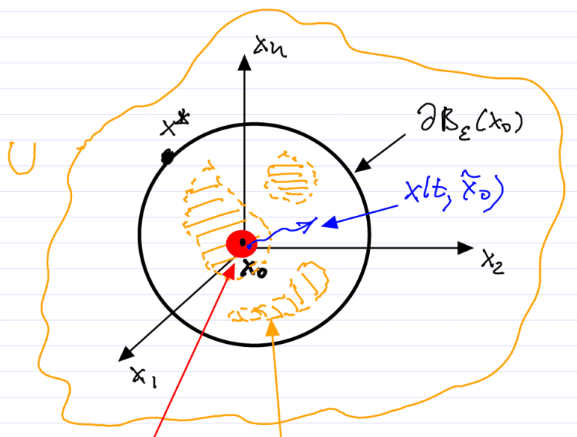
\includegraphics[width=0.45\textwidth]{figures/ch2/22lyap_pf_1.png}
	\caption{The constellation of $U$, $U_\varepsilon$, $\partial B_{\varepsilon}(x_0)$, and $B_{\delta(\varepsilon)}(x_0)$ from the proof of Lyapunov's direct method. The red arrow points at $B_{\delta(\varepsilon)}(x_0)$ and the yellow arrow at a connected component of $U_\varepsilon$.}
	\label{fig:lyap_pf_1}
\end{figure}

Now observe that for every $\tilde{x}_{0} \in B_{\delta(\varepsilon)}(x_0)$ we have that along trajectories $V(x(t; \tilde{x}_{0})) \leq V(\tilde{x}_{0}) < \alpha(\varepsilon)$. The first inequality comes from hypothesis (ii) and the second inequality from the definition of $U_{\varepsilon}$. This implies that for $x(t; \tilde{x}_0) \in U_{\varepsilon}$ we have that $x(t; \tilde{x}_{0})$ is not in $\partial B_{\varepsilon}(x_0)$ for any $t> 0$. The trajectory $x(t; \tilde{x}_0)$ is continuous, in order for it to leave the ball $B_{\varepsilon}(x_0)$ it must intersect the boundary $\partial B_{\varepsilon}(x_0)$. At this point $V(x)$ will atain a value of at least $\alpha(\varepsilon)$ by definition, however this is in contradiction to the fact that $V(x(t;\tilde{x}_0))$ is strictly smaller that $\alpha(\varepsilon)$. Therefore must stay in the ball $B_{\varepsilon}(x_0)$ for all times.
\end{proof}

Now we present some extensions to this theorem for various different stability types. These are necessary, as the previous theorem only provides a sufficient condition for stability (it is not ``if and only if").

\begin{theorem}[Theorem 2]
Consider the same dynamical system. Assume
\begin{enumerate}
	\item $V(x)$ is positive definite,
	\item $\dot{V}(x)$ is negative definite, i.e.
		\begin{align}
			\dot{V}(x) < 0,\ x\in U- \{x_0\}.
		\end{align}
\end{enumerate}
		Then $x=x_0$ is asymptotically stable. These hypotheses are illustrated in Fig. \ref{fig:lyap_thm2_hypos}.
\end{theorem}
\begin{figure}[h!]
	\centering
	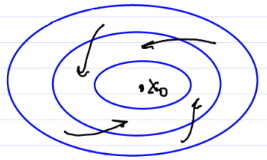
\includegraphics[width=0.4\textwidth]{figures/ch2/24lyap_thm2_hypos.png}
	\caption{The hypotheses of Theorem 2 illustrated, the key difference being that the arrows (denoting the flow of the dynamical system) cross the level surfaces of $V$ (blue rings) toward $x_0$.}
	\label{fig:lyap_thm2_hypos}
\end{figure}

\begin{theorem}[Theorem 3]
	Consider the same dynamical system. Assume
	\begin{enumerate}
		\item $V(x)$ is positive definite,
		\item $\dot{V}(x)$ is positive definite, i.e.
		\begin{align}
			\dot{V}(x)>0,\ x\in U- \{x_0\}.
		\end{align}
	\end{enumerate}
	Then $x=x_0$ is unstable. The hypotheses are illustrated in Fig. \ref{fig:lyap_thm3_hypos}.
\end{theorem}

\begin{figure}[h!]
	\centering
	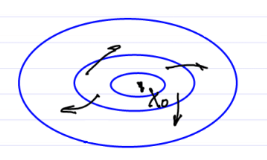
\includegraphics[width=0.4\textwidth]{figures/ch2/25lyap_thm3_hypos.png}
	\caption{The hypotheses of Theorem 3 illustrated, the key difference being that the arrows (denoting the flow of the dynamical system) cross the level surfaces of $V$ (blue rings) away from $x_0$.}
	\label{fig:lyap_thm3_hypos}
\end{figure}

\begin{theorem}[Theorem 4]
	Consider the same dynamical system. Assume
	\begin{enumerate}
		\item $V(x)$ is indefinite, i.e. arbitrarily close to $x_0$ there exists $a,b \in U$ such that $V(x_1)\cdot V(x_2) <0$ (they have opposite signs and are not equal to 0) and $V(x_0)=0$. Furthermore, this is a critical point, i.e. $DV(x_0)=0$.
		\item $\dot{V}(x)$ is definite near $x_0$ (either positive or negative).
	\end{enumerate}
	Then $x=x_0$ is unstable. The geometry of the hypotheses are  illustrated in Fig. \ref{fig:lyap_thm4_hypos}.
\end{theorem}

\begin{figure}[h!]
	\centering
	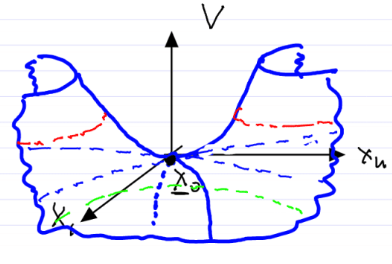
\includegraphics[width=0.4\textwidth]{figures/ch2/26lyap_thm4_hypos.png}
	\hspace{0.05\textwidth}
	\includegraphics[width=0.4\textwidth]{figures/ch2/26lyap_thm4_hypos2.png}
	\caption{The geometry of hypotheses (i) (left) and (ii) (right) for $\dot{V}$ positive definite of Theorem 4 illustrated. On the right level surfaces are designated by lines, blue corresponds to $V=0$, red $V>0$, and green $V<0$, which can be seen as the dotted lines of the same colors on the left.}
	\label{fig:lyap_thm4_hypos}
\end{figure}

\begin{remark}[]
	In each of these theorems, the definiteness of $ \dot{V}$ can be replaced by semidefiniteness, if we add that the set $\{x\in U:\ \dot{V}(x)=0 \}$ does not contain full trajectories of the system. This is called Krasovsky's condition.
\end{remark}

Now we would like to put these theorems into practice with a few examples.
\begin{ex}[Stability analysis of the pendulum with Lyapunov's direct method]
	Recall that using linearization, we were only able to conclude the stability type of one of the fixed points for the dynamical system of the pendulum
	\begin{align}
		ml^2 \ddot{\varphi} + mgl \sin(\varphi) =0.
	\end{align}
Now we will use the energy as a Lyapunov function, which is often very useful. The energy is given by
\begin{align}
	E(x) = E(\varphi, \dot{\varphi}) = \frac{1}{2}ml^2 \dot{\varphi}^2 + mgl(1-\cos(\varphi)) 
	= \frac{1}{2}ml^2 \dot{x_2}^2 + mgl(1-\cos(x_1)).
\end{align}
Transforming the dynamical system to be an system of first order ODEs we obtain
\begin{align}
	x = 
	\begin{pmatrix}
		x_1 \\x_2
	\end{pmatrix}
	=
	\begin{pmatrix}
		\varphi \\ \dot{\varphi}
	\end{pmatrix}
	;\quad \dot{x}=
	\begin{pmatrix}
		\dot{x_1} \\ \dot{x_2}
	\end{pmatrix}
	=
	\begin{pmatrix}
		x_2 \\ - \frac{g}{l} \sin (x_1)
	\end{pmatrix}
	=f(x).
\end{align}
At the fixed point $x=(0,0)$ we have
\begin{align}
	E(0,0) = 0;\quad DE(0,0) = 0\in \mathbb{R}^{2\times 2};\quad D^2E(0,0) =
\begin{pmatrix}
	mgl & 0 \\
	0 & ml^2
\end{pmatrix}.
\end{align}
We have that the Hessian of $E$ is positive definite. Therefore $E$ is positive definite at $(0,0)$. Further we have
\begin{align}
	\dot{E}(x) = \langle DE(x), f(x) \rangle 
	=
	\begin{pmatrix}
		mgl \sin(x_1) &  ml^2 x_2
	\end{pmatrix}
	\begin{pmatrix}
		x_2 \\ - \frac{g}{l}\sin (x_1)			
	\end{pmatrix}
	= 0.	
\end{align}
Thus $\dot{E}$ is negative semidefinite. Now the hypotheses of Theorem \ref{thm:direct} are fulfilled, hence $x=(0,0)$ is Lyapunov stable. Importantly, this is a nonlinear result and we did not need to refer to the linearization of the system!

At the fixed point $x = (\pi, 0)$. We check again using the energy. First we realize that $E(\pi, 0)= 2mgl$, so we subtract the constant and redefine to obtain $\tilde{E}= E - 2mgl$. Now $\tilde{E}(\pi, 0) = 0$, although this is not essential. Next we calculate
\begin{align}
	DE(\pi, 0) = 0\in \mathbb{R}^{n\times n};\quad D^2E(\pi, 0) = 
	\begin{pmatrix}
		-mgl & 0 \\
		0 & ml^2
	\end{pmatrix}
	.
\end{align}
Hence, $E$ is indefinite at $(\pi, 0)$. From the previous calcuation we alread know that $\dot{E}(\pi, 0) = 0$, i.e. $\dot{E}$ is semidefinite. We cannot apply Theorem 4, but linearization already concluded that $(\pi,0)$ was unstable.

If we add damping the dynamics becomes
\begin{align}
	m\ell^2 \ddot{\varphi} + c \dot{\varphi} mg\ell \sin(\varphi) =0.
\end{align}
Again we transform the system by introducing the coordinates $x_1 =\varphi$ and $x_2=\dot{\varphi}$. Thus we have a first order ODE
\begin{align}
	\begin{dcases}
		\dot{x_1} = x_2 \\
		\dot{x_2} = - \frac{c}{m\ell^2}x_2 - \frac{g}{\ell}\sin(x_1).
	\end{dcases}
\end{align}
We still have the fixed points $(0,0)$ and $(0, \pi)$ and the energy $E = \frac{1}{2}m \ell^2 \dot{\varphi}^2 + mg \ell(1 - \cos(\varphi))$. Again we find
\begin{align}
	DE =
	\begin{pmatrix}
		mg\ell \sin(x_1) \\ m \ell^2 x_2
	\end{pmatrix}
	\implies DE(0) = 0;\quad
	D^2E =
	\begin{pmatrix}
		mg\ell \cos(x_1) & 0 \\
		0 & m \ell^2
	\end{pmatrix}
	.
\end{align}
Thus $E$ is positive definite at $(0,0)$ and indefinite at $(0, \pi )$. We have
\begin{align}
	\dot{E} = DE \cdot f = mgl \sin(x_1)x_2 + m\ell^2 x_2 \left(-\frac{c}{m\ell^2}x^2 - \frac{g}{\ell}\sin(x_1)\right) = - cx_2^2.
\end{align}
Note here that $\dot{E}= -cx_2^2$ is only negative semi-definite. Therefore the asymptotic stability of $x=(0,0)$ and the instability of $x=(0,\pi )$ do not follow from theorems 1 or 4. However, the set $S=\left\{x:\ \dot{E}(x)=0\right\} - \left\{(0,0),\ (0,\pi )\right\}$ does \underline{not} contain full trajectories. Indeed
\begin{align}
	\left.\frac{d}{dt}x_2(t)\right|_{x=0} = -\frac{g}{\ell}\sin(x_1) \neq 0,\ x\in S.
\end{align}
Hence, the asymptotic stability of $(0,0)$ and instability of $(0,\pi )$ follows by Krasovsky's condition.
\end{ex}
 \begin{ex}[Stability analysis of the friction pendulum]
	 We have a shaft which is constantly rotating with angular speed $\Omega $, around this shaft is a sleeve which rubs against the shaft creating friction. To this sleeve is a mass $m$ attached at distance $l$, the deflection of this mass from its standard position (directly below the shaft) is measured by $\varphi$. The gravity constant is given by $g$. This setup is depicted in Fig. \ref{fig:friction_pend}.
\begin{figure}[h!]
	\centering
	\includegraphics[width=0.4\textwidth]{figures/ch2/27friction_pend.png}
	\caption{The setup of the friction pendulum.}
	\label{fig:friction_pend}
\end{figure}
The torque driving the pendulum is given by 
\begin{align}
	T(\dot{\varphi}) = T_0  \textrm{sign}(\Omega - \dot{\varphi}).
\end{align}
From this we get the equation of motion
\begin{align}
	ml^2 \ddot{\varphi} + mgl \sin(\varphi) = T(\dot{\varphi}) = T_0  \textrm{sign} (\Omega - \dot{\varphi}).
\end{align}
By assuming $\Omega \gg 1$, i.e. very fast rotation of the shaft, we find that $T(\dot{\varphi}) = T_0$. Next we transform the coordinates in order to get an ODE
\begin{align}
	\begin{pmatrix}
		x_1 \\ x_2
	\end{pmatrix}
	=
	\begin{pmatrix}
		\varphi \\ \dot{\varphi}
	\end{pmatrix}
	;\quad
	\begin{pmatrix}
		\dot{x}_1 \\ \dot{x_2}
	\end{pmatrix}
=
\begin{pmatrix}
	x_2 \\ - \frac{g}{l} \sin(x_1) + \frac{T_0}{ml^2}
\end{pmatrix}
.
\end{align}
Thus the fixed point $x_0$ is at $(\overline{x}_1, \overline{x}_2)$ given by 
\begin{align}
	\sin(\overline{x}_1) = \frac{T_0}{mgl};\quad \overline{x}_2=0.
\end{align}
Since the system is forced, energy is not conserved and we cannot use it as a Lyapunov function. However, there may still exist a conserved quantity. Consider using
\begin{align}
	V(x) = \left[  \textrm{total energy at time } t \right] - \left[  \textrm{work put in between time } t  \textrm{ and } t_0 \right] = \left[ \textrm{initial energy} \right] =  \textrm{const.}  
\end{align}
This is a conserved quantity in all mechanics problems, but generally cannot be calculated without already knowing the trajectories. Here we can, as
\begin{align}
	V(x(t)) = \frac{1}{2} ml x_2^2 + mgl(1- \cos(x_1)) - T_0(\underbrace{x_1}_{\varphi(t)} - \underbrace{x_1(0)}_{\varphi(0)}).
\end{align}
We can drop the constant term $T_0 x_1(0)$. Now verify that $V$ is indeed constant
\begin{align}
	\dot{V}(x) = \frac{\partial V}{\partial x_1} \dot{x}_1 + \frac{\partial V}{\partial x_2} \dot{x}_2 = \left( mgl \sin(x_1) - T_0\right) x_2 + ml^2x_2 \left( - \frac{g}{l}\sin(x_1) + \frac{T_0}{ml^2} \right) = 0.
\end{align}
Hence $\dot{V}(x)$ is semidefinite, and may be used to conclude stability or instability. We must check the Lyapunov conditions for $V(x)$ 
\begin{subequations}
\begin{align}
	DV(x_0) &= 
\begin{pmatrix}
	mgl \sin(\overline{x}_1) - T_0 & ml^2 \overline{x}_2
\end{pmatrix}
=
\begin{pmatrix}
	0& 0
\end{pmatrix}
\\
D^2V(x_0) &= 
\begin{pmatrix}
	mgl \cos(\overline{x}_1) & 0 \\
	0 & ml^2
\end{pmatrix}.
\end{align}\end{subequations}
The Hessian is positive definite as long as $\overline{x}_1 \in \left(-\frac{\pi }{2}, \frac{\pi }{2}\right)$, and all fixed points in this region are stable by Theorem \ref{thm:direct}. The Hessian is indefinite if $\overline{x}_1 \not \in \left[-\frac{\pi }{2}, \frac{\pi }{2}\right]$, but in this case Theorem 4 is not applicable as $\dot{V}$ is not definite. More detailed discussion and further results on Lyapunov's direct method can be found in \cite{LiapunovDirect}.
 \end{ex}
 

\newpage

\chapter{Bifurcations of fixed points}
\section{Local nonlinear dynamics near fixed points}
We are interested in the local nonlinear dynamics around fixed points. Consider
\begin{align}
	\dot{x}=f(x);\quad f\in \mathcal{C}^{r},r \geq 1; \quad f(p) = 0, \numberthis \label{eq:4star}
\end{align}
i.e. $p$ is a fixed point of the dynamical system. The linearized system at $p$ is
\begin{align}
	\dot{y} = Df(p)y,\ y\in \mathbb{R}^{n},\ Df(p)\in \mathbb{R}^{n \times n}. \numberthis \label{eq:4sstar}
\end{align}
The linearization has the eigenvalues $\lambda_1, \ldots, \lambda_n \in \mathbb{C}$ with multiplicities counted. Corresponding to these eigenvalues are the eigenvectors $e_1,\ldots,e_n \in \mathbb{C}^{n}$, including generalized eigenvectors for when the algebraic multiplicity is greater than the geometric multiplicity. The eigenvector $e_j$ is real when $\lambda_j \in \mathbb{R}$.

\begin{definition}
The following subspaces are invariant for the linearized dynamical system:
\begin{enumerate}
	\item The \emph{stable subspace}
		\begin{align}
			\boxed{
				E^{S} =  \textrm{span} _{j}\left \{  \textrm{Re} (e_j),  \textrm{Im} (e_j):\  \textrm{Re} (e_j) < 0\right\},
			}
		\end{align}
	\item The \emph{unstable subspace}
		\begin{align}
			\boxed{
				E^{U} =  \textrm{span} _{j}\left \{  \textrm{Re} (e_j),  \textrm{Im} (e_j):\  \textrm{Re} (e_j) > 0\right\},
			}
		\end{align}
	\item The \emph{center subspace}
		\begin{align}
			\boxed{
				E^{C} =  \textrm{span} _{j}\left \{  \textrm{Re} (e_j),  \textrm{Im} (e_j):\  \textrm{Re} (e_j) = 0\right\}.
			}
		\end{align}
\end{enumerate}

\end{definition}
\begin{remark}[]
	Note here that the following facts hold
	\begin{enumerate}
		\item $E^{C}= \emptyset$ if and only if $p$ is hyperbolic,
		\item $E^{U,S}$ and $E^{C}$ are invariant subspaces of \eqref{eq:4sstar} by construction,
		\item Solutions of \eqref{eq:4sstar} in $E^{S}$ (resp. $E^{U}$) decay to $y=0$ as $t \to \infty$ (resp. $t \to - \infty$). 
	\end{enumerate}
	
\end{remark}

We now discuss what happens to these subspaces in the nonlinear system \eqref{eq:4star}.
\begin{theorem}[Center Manifold Theorem] \label{thm:center_mfd}
	The following hold:
	\begin{enumerate}
		\item There exists a unique \emph{stable manifold} $W^{S}(p)$ for \eqref{eq:4star}, such that
	\begin{itemize}
		\item $W^{S}(p)$ is a $\mathcal{C}^{r}$ manifold (surface), tangent to $E^{S}$ at $p$ with $ \textrm{dim } W^{S}(p) =  \textrm{dim } E^{S}$,
		\item $W^{S}(p)$ is invariant for \eqref{eq:4star} and for $x\in W^{S}(p)$ we have 
			\begin{align}
				\| F^{t}(x)-p \| \leq K_{S} \exp\left[ t \left( \max_{ \textrm{Re} (\lambda_j) < 0}( \textrm{Re} (\lambda_j)) + \varepsilon_S \right) \right]
			\end{align}
	 for $t\geq 0$, $0 < \varepsilon_S \ll 1$, and  $\| x- p\|$ small enough.
	\end{itemize}
			
		\item There exists a unique \emph{unstable manifold} $W^{U}(p)$ for \eqref{eq:4star}, such that
	\begin{itemize}
		\item $W^{U}(p)$ is a $\mathcal{C}^{r}$ manifold (surface), tangent to $E^{U}$ at $p$ with $ \textrm{dim } W^{U}(p) =  \textrm{dim } E^{U}$,
		\item $W^{U}(p)$ is invariant for \eqref{eq:4star} and for $x\in W^{U}(p)$ we have 
			\begin{align}
				\| F^{t}(x) -p\| \leq K_{U} \exp\left[ t \left( \max_{ \textrm{Re} (\lambda_j) > 0}( \textrm{Re} (\lambda_j)) + \varepsilon_U \right) \right]
			\end{align}
	 for $t\leq 0$, $0 < \varepsilon_U \ll 1$, and  $\| x- p\|$ small enough.
	\end{itemize}
			
\item There exists a (not necessarily unique) \emph{center manifold} $W^{C}(p)$ for \eqref{eq:4star}, such that
	\begin{itemize}
		\item $W^{C}(p)$ is a $\mathcal{C}^{r-1}$ manifold (surface), tangent to $E^{C}$ at $p$ with $ \textrm{dim } W^{C}(p) =  \textrm{dim } E^{C}$,
	\end{itemize}
			
	\end{enumerate}
	
\end{theorem}
The geometry of these manifolds and their corresponding subspaces are sketched in Fig. \ref{fig:mfds_def}.
\begin{figure}[h!]
	\centering
	\includegraphics[width=0.6\textwidth]{figures/ch3/1manifolds_def.png}
	\caption{A sketch of the stable (red), unstable (blue), and center manifolds (green), along with their respective linear subspaces, that are invariant under the linearized dynamics. Note the existence of multiple center manifolds and the unique unstable/stable manifolds.}
	\label{fig:mfds_def}
\end{figure}

Notice that Theorem \ref{thm:center_mfd} does not state anything  about the asymptotic dynamics on the center manifold, in contrast to that of the unstable and stable manifolds. This means that the overall dynamics depends crucially on the center manifold. In the case when $W^u=\emptyset$, even the stability type of the fixed point is determined by $W^C(p)$. This is why it will be the subject of further investigations.

\section{The center manifold}
\begin{ex}[Uniqueness of the center manifold]
	Since Theorem 4.2 gave no guarantees on the uniqueness of the center manifold, now we explore this non-uniqueness in an example.
	\begin{align}
\begin{dcases}
	\dot{x} = x^2 \\
	\dot{y} = -y.
\end{dcases}
	\end{align}
	First, linearize at the origin to find the linearized dynamics
	\begin{align}
		A = Df(0) = 
		\begin{pmatrix}
			0 & 0 \\ 0 & -1
		\end{pmatrix}
		.
	\end{align}
	The linearized dynamics is illustrated in Fig. \ref{fig:cmfd_lin_ex}. We find the invariant subspaces
	\begin{align}
		E^{C} =  \textrm{span}\left\{ 
			\begin{pmatrix}
				1 \\ 0 
			\end{pmatrix}
		\right\};\quad
		E^{S} =  \textrm{span}  \left\{
			\begin{pmatrix}
				0 \\ 1
			\end{pmatrix}
		\right\}; \quad
		E^{U} = \emptyset.
	\end{align}
	The nonlinear manifolds are illustrated with the invariant subspaces from the linearization in Fig. \ref{fig:cmfd_lin_ex}.
	\begin{figure}[h!]
		\centering
		\includegraphics[width=0.45\textwidth]{figures/ch3/2cmfd_lin_ex.png}
		\includegraphics[width=0.4\textwidth]{figures/ch3/3cmfd_nonlin_ex.png}
		\caption{Left: The linearized dynamics around the origin. Right: The nonlinear phase portrait. }
		\label{fig:cmfd_lin_ex}
	\end{figure}
	Observe that there exist infinitely many center manifolds which are all invariant and all tangent to $E^{C}$ at the origin. We also see that although the fixed point at the origin is stable in the linearized system, it is unstable in the nonlinear system.
\end{ex}

We now present a method to calculate $W^C(p)$ in general cases.
\begin{enumerate}
	\item Consider 
		\begin{align}
			\dot{z} = F(z); \quad F(0) = 0;\quad z \in \mathbb{R}^{c+d};\quad F \in \mathcal{C}^{r},
		\end{align}
	where $c$ represents the number of center directions at the origin ($ \textrm{dim }E^{C}$) and $d$ denotes the remaining directions ($ \textrm{dim } E^{U} +  \textrm{dim } E^{S}$).
	\item Now block-diagonalize the linearization. This consists of four steps
		\begin{enumerate}
			\item First linearize the dynamics to find $\dot{z} = Mz + \mathcal{O}(\|z\|^2)$ with $M = DF(0) \in \mathbb{R}^{(c+d) \times (c+d)}$.
			\item Define the transformation matrix
				\begin{align}
					T=
					\begin{bmatrix}
						a_1 & \ldots & a_c & b_1 & \ldots & b_d	
					\end{bmatrix}
				=
				\begin{bmatrix}
					\textrm{basis in } E^{C} &  \textrm{basis in } E^{U} \oplus E^{S}
				\end{bmatrix}
				.
				\end{align}
			\item Pass to the basis from the transformation matrix by introducing a new set of coordinates as $z = T \xi$
				\begin{align}
					\dot{\xi} = T^{-1}\dot{z} = T^{-1}MT \xi + T^{-1}\mathcal{O}(\| T\xi\|^2) = 
					\begin{pmatrix}
						A & 0 \\
						0 & B
					\end{pmatrix}
					\xi + \mathcal{O}(\| \xi \| ^2).
				\end{align}
			The matrices $A$ and $B$ are elements of $\mathbb{R}^{c \times c}$ and $\mathbb{R}^{d \times d}$ respectively.	
		\item Let $\xi = 
			\begin{pmatrix}
				x \\ y
			\end{pmatrix}
			\in \mathbb{R}^{c}\times \mathbb{R}^{d}$, the $x$-coordinates are aligned with $E^{C}$ and the $y$-coordinates are perpendicular to them. We then find
			\begin{align}
				\dot{x} = Ax + f(x,y);\quad \dot{y} = By + g(x,y), \numberthis \label{eq4:trafod_eqn}
			\end{align}
			for $f,g \in \mathcal{C}^{r}$ and $f,g = \mathcal{O}(\|x\|^2, \|y\|^2, \|x\|\|y\|)$. The geometry in these coordinates is depicted in Fig. \ref{fig:cmfd_trafo_geom}. The center manifold is given by
			\begin{align}
				W^{C}(0) = \left\{ (x,y) \in U:\ y = h(x)\right\}
			\end{align}
			for $h:\mathbb{R}^{c} \to \mathbb{R}^{d}$ and $ h \in \mathcal{C}^{r-1}$ as in the theorem.
			\begin{figure}[h!]
				\centering
				\includegraphics[width=0.4\textwidth]{figures/ch3/4cmfd_trafo_geom.png}
				\caption{The geometry of the nonlinear system in the transformed coordinates aligned with the invariant subspaces of the linearization. The blue arrow points to the center manifold $W^{C}(0)$.}
				\label{fig:cmfd_trafo_geom}
			\end{figure}
		\end{enumerate}
	\item Now we use the invariance of $W^{C}(0)$, i.e. for all $t$, it holds that $y(t) = h(x(t))$. With this we find
		\begin{align}
			\dot{y} = Dh(x(t)) \dot{x}(t).
		\end{align}
		We can now substitute $\dot{x}$ and $\dot{y}$ from \eqref{eq4:trafod_eqn} to get the following nonlinear partial differential equation (PDE) for $h(x)$
\begin{align}
	\boxed{
		Bh(x) + g(x, h(x)) = Dh(x) \left[ Ax + f(x, h(x))\right] \numberthis \label{eq4:1star}.
	}
\end{align}
In addition to \eqref{eq4:1star} being nonlinear, the boundary conditions are also  unknown. Therefore there is little hope for solving it analytically.
\item Instead take the Taylor expansion of \eqref{eq4:1star} to approximate the solution
	\begin{align}
		h(x) = \underbrace{h(0)}_{=0} + \underbrace{Dh(0)}_{=0}x + \frac{1}{2} \underbrace{D^2h(0)}_{3- \textrm{tensor} } \otimes x \otimes x + \mathcal{O}(\|x \| ^3),
	\end{align}
	where the first two terms are 0 due to the tangency to $E^{C}$ at $0$. We therefore have that $h = O(x^2)$ and we are justified in seeking $W^C(0)$ in this form. We can then restrict the system to the center manifold by substituting $y = h(x)$ to get the reduced dynamics as 
	\begin{align}
		\boxed{
			\dot{x}=Ax+f(x,h(x)).
		}
	\end{align}
\end{enumerate}

\begin{ex}[Finding the center manifold]
	Consider the dynamical system
	\begin{align}
		\begin{dcases}
			\dot{x}=xy \\
			\dot{y}=-y+\alpha x.
		\end{dcases}	
	\end{align}
	First we linearize at $(0,0)$ to get 
	\begin{align}
		M =
		\begin{pmatrix}
			[0] & [0] \\
			[0] & [-1]
		\end{pmatrix}
	\end{align}
	which is already in block-matrix form. The dimensions of the stable, unstable, and center subspaces of the linearization are 1, 0, and 1 respectively. Hence the stability type depends on the dynamics on the center manifold $W^{C}(0)$. We now look for a parameterization of $W^{C}(0)$ in the form
	\begin{align}
		h(x) = ax^2 + bx^3 + cx^4 + \mathcal{O}(x^5).
	\end{align}
	Since the right-hand side of the dynamical system was $\mathcal{C}^\infty$, this expansion could formally be continued to any order. However, the expansion will not converge as that would imply the uniqueness of the center manifold. In this example, we work with a finite, order 4 truncation. Now use the invariance (the PDE \eqref{eq4:1star} we derived above) to find
	\begin{align}
		\dot{y} = h'(x)\dot{x} = \left[2ax+3bx^2 + 4cx^3 + \mathcal{O}(x^4) \right] x \left[ax^2+bx^3+cx^4 + \mathcal{O}(x^5) \right]. \numberthis \label{eq4:one}	
	\end{align}
	On the other hand, from the dynamical system we know
	\begin{align}
		\dot{y}=-h(x) + \alpha x^2 =(\alpha - a) x^2 -bx^3 - cx^4 + \mathcal{O}(x^5). \numberthis \label{eq4:two}
	\end{align}
	Equations \eqref{eq4:one} and \eqref{eq4:two} must hold for all $x$ small enough, therefore the coefficients of equal powers of $x$ in these two equations must match.
	\begin{subequations}
	\begin{align}
		\mathcal{O}(x^2)&:\ \alpha = a\\
		\mathcal{O}(x^3)&:\ b=0 \\
		\mathcal{O}(x^4)&:\ 2a^2 = -c.
	\end{align}\end{subequations}
	Therefore we find 
	\begin{align}
		\boxed{
	h(x) =\alpha x^2 - 2\alpha^2x^4 + \mathcal{O}(x^5).}
	\end{align}
	Then the dynamics on $W^{C}(0)$ becomes
	\begin{align}
		\boxed{
			\dot{x}= xh(x) = \alpha x^3(1-2\alpha x^2) + \mathcal{O}(x^6). \numberthis \label{eq4:2star}
		}
	\end{align}
	The dynamics is depicted in Fig. \ref{fig:cmfd_alpha_diff}. For $\alpha > 0$ the origin is unstable, meanwhile for $ \alpha <0$ the origin is asymptotically stable.
	\begin{figure}[h!]
		\centering
		\includegraphics[width=0.8\textwidth]{figures/ch3/5cmfd_alpha_diff}
		\caption{Left: The nonlinear dynamics on the center manifold for $\alpha > 0$. Right: The nonlinear dynamics on the center manifold for $\alpha < 0$.}
		\label{fig:cmfd_alpha_diff}
	\end{figure}
	
	The full local stable manifold for $\alpha <0$ is $\overline{W}^{S}(0)=U$ and it is of dimension 2. The difference between $\overline{W}^{S}(0)$ and $W^{S}(0)$ is that in general the decay rate in $\overline{W}^{S}(0)-W^{S}(0)$ is generally weaker than the rate guaranteed in the Center Manifold Theorem. 

\begin{remark}[]
	The $\mathcal{O}(x^5)$ truncation has two hyperbolic fixed points at $x = \pm \frac{1}{\sqrt{2 \alpha} }$, however the full system has no such fixed points. The reason for this is that away from the origin, the $\mathcal{O}(x^6)$ terms are no longer guaranteed to be small relative to the $\mathcal{O}(x^5)$ terms, and the truncation this far away from 0 is not justified.
\end{remark}
\end{ex}

After this example we would like to explore if the concept of the center manifold is robust, as the existence of eigenvalues with $ \textrm{Re} (\lambda_i) = 0$ is not. We will explore this in an example.

\begin{ex}[Perturbing the previous example]
	Consider the following perturbed dynamical system
	\begin{align}
		\begin{dcases}
			\dot{x} = xy + \varepsilon x \\
			\dot{y} = -y + \alpha x^2
		\end{dcases}
;\quad |\varepsilon | \ll 1.
	\end{align}
The linearization of this system yields
\begin{align}
	\begin{dcases}
		\dot{x} = \varepsilon x \\
		\dot{y} = -y.
	\end{dcases}
\end{align}
Now the center manifold disappears as the center subspace $E^{C}$ disappears for $\varepsilon>0$!
\end{ex}

\section{Center manifolds depending on parameters}
We begin with the setup
\begin{subequations}
\begin{align}
	\begin{dcases}
		\dot{x} = Ax + f(x,y,\varepsilon) \\
		\dot{y} = By + g(x,y,\varepsilon)
	\end{dcases}
;\quad x \in \mathbb{R}^{c},\ y \in \mathbb{R}^{d},\ 0\leq \|\varepsilon\| \ll 1;\ \varepsilon\in \mathbb{R}^{p};\\
f,g \in \mathcal{C}^{r},\ f,g=\mathcal{O}(\|x\|^2, \|y\|^2, \|x\|\|x\|, {\|\varepsilon\| \|x\|, \|\varepsilon\| \|y\|} ).
\end{align}\end{subequations}
The order $\|\varepsilon\| \|x\|$ and $\|\varepsilon\| \|y\|$ terms are due to the perturbation of the linear part. Now assume $ \textrm{Re} (\lambda _j(A))= $ for $j=1,\ldots,c$ (the center directions) and $ \textrm{Re} (\lambda _j(B)) \neq  $ for $j=1,\ldots,d $ (the hyperbolic directions). Next, rewrite $\tilde{x}=
\begin{pmatrix}
	x \\ \varepsilon
\end{pmatrix}
$ and $\tilde{y}=y$ to obtain the system
\begin{align}
	\begin{dcases}
		\dot{\tilde{x}} = \tilde{A}\tilde{x} + \tilde{f}(\tilde{x}, \tilde{y}) \\
		\dot{\tilde{y}} = \tilde{B}\tilde{y} + \tilde{g}(\tilde{x}, \tilde{y}) 
	\end{dcases}
	;\quad \tilde{A}=
	\begin{pmatrix}
		A & 0 \\ 0 & 0	
	\end{pmatrix}
	\in \mathbb{R}^{(c+p)\times (c+p)}; \quad \tilde{f} =
	\begin{pmatrix}
		f \\ 0
	\end{pmatrix}. \numberthis \label{eq4:unostar}
\end{align}
Here, $\tilde{g}=g$ and $\tilde{B}=B$. Further, note that $ \textrm{span} \left\{
	\begin{pmatrix}
		x \\0
	\end{pmatrix}
\right\}$ is an invariant subspace for $\tilde{A}$. The eigenvalues of $\tilde{A}$ are the same as those of $A$ and an additional $0$, thus there are $c+p$ center directions and $d$ hyperbolic directions. Applying the center manifold theorem to the fixed point $0 \in \mathbb{R}^{c+p+d}$ of \eqref{eq4:unostar} we obtain that there exists a $\mathcal{C}^{r-1}$ manifold $\tilde{W}^{C}(0)$ tangent to $E^{C}$ at $
\begin{pmatrix}
	\tilde{x} \\ \tilde{y}
\end{pmatrix}
= 
\begin{pmatrix}
	0 \\ 0
\end{pmatrix}
$ which is invariant and is of dimension $c+p$. The geometry of this manifold is illustrated in Fig. \ref{fig:pert_cent_mfd}. Note in the figure that there is no dynamics in the $\varepsilon$ direction, as $\dot{\varepsilon}=0$ and that $(x,y)=(0,0)\in \mathbb{R}^{c+d}$ remains a fixed point for $\varepsilon\neq 0$.
\begin{figure}[h!]
	\centering
	\includegraphics[width=0.7\textwidth]{figures/ch3/6pert_cent_mfd.png}
	\caption{Geometry of the center manifold with the perturbation. The straight red arrow designates the cut at $\varepsilon=0$ which is equal to $W^{C}(0)$, the squiggly red arrow points at the continuation of the center manifold from $\varepsilon=0$ to $\varepsilon \neq 0$.}
	\label{fig:pert_cent_mfd}
\end{figure}

Computing $\tilde{W}^{C}(0)$ is done in a similar fashion as before. We use the center manifold theorem to get	
\begin{align}
	\tilde{y} = y= \tilde{h}(\tilde{x}) = \tilde{h}(x,\varepsilon) = \mathcal{O}(\|x\|^2, \|\varepsilon \|\|x\|, \|\varepsilon\|^2) = \mathcal{O}(\|x\|^2, \|\varepsilon \|\|x\|).
\end{align}
The order $\|\varepsilon\|^2$ term was dropped as $x=0$ must remain a fixed point. The function $h$ describes the graph of $W^{C}_{\varepsilon}(0)$. Then the reduced dynamics on $W^{C}_{\varepsilon}(0)$ is
\begin{align}
	\boxed{
		\dot{x} = Ax + f(x, \tilde{h}(x, \varepsilon), \varepsilon).
}
\end{align}
This can then be applied to the perturbed example from above.

\begin{ex}[Revisting the perturbation]
	Recall the dynamical system
	\begin{align}
		\begin{dcases}
			\dot{x} = xy + \varepsilon x\\
			\dot{y} = -y + \alpha x^2.
		\end{dcases}
	\end{align}
	We have the persisting fixed point at $(x,y)=(0,0)\in \mathbb{R}^{c+d}$	and the system is already in standard form with 
	 \begin{align}
		 A=0;\quad B=-1;\quad f(x,y,\varepsilon) = xy + \varepsilon x;\quad g(x,y,\varepsilon) = -\alpha x^2.
	\end{align}
	We apply the center manifold theorem and get the existence of $W^{C}_{\varepsilon}(0)$ for $|\varepsilon|\ll 1$. This manifold satisfies
	 \begin{align}
		 y = \tilde{h}(x,\varepsilon) = ax^2 + bx\varepsilon + c\varepsilon^2
		 +dx^3 + ex^2 \varepsilon +j x\varepsilon^2 + k\varepsilon ^3
		 +lx^4. \ldots \numberthis \label{eq4:juanstar}
	\end{align}
	The term $c\varepsilon^2$ must be equal to 0 for all $\varepsilon$ such that the fixed point persists, therefore $c=0$. Next the invariance $y(t) = \tilde{h}(x(t)), \varepsilon)$ is used, taking the time derivative on both sides yields
	\begin{align}
	\dot{y} = \left[2ax + b\varepsilon + \mathcal{O}(2) \right]
	\underbrace{\left[\mathcal{O}(3) + \varepsilon x \right]} _{=\dot{x}  \textrm{ from ODE and \eqref{eq4:juanstar} }}
		= 2a \varepsilon x^2 + b\varepsilon^2 x  + \mathcal{O}(4).
	\end{align}
	The $\mathcal{O}(n)$ designates terms of total degree $n$, for example $x^n$ or $x^{n-k}\varepsilon^{k}$. From the ODE we find
	\begin{align}
		\dot{y} = -y + \alpha x^2 
		= -ax^2 -bx\varepsilon - c\varepsilon^2 - dx^3 - e x^2 \varepsilon - j x \varepsilon^2 -k \varepsilon^3 - \mathcal{O}(4) + \alpha x^2.
	\end{align}
	Comparing equal powers in these two equations we find
	\begin{subequations}
	\begin{align}
		\mathcal{O}(x^2)&:\ 0 = \alpha -a; \quad
		&\mathcal{O}(\varepsilon^2)&:\ 0=-c;\quad
         	&\mathcal{O}(x\varepsilon)&:\ 0=-b; \\
		\mathcal{O}(\varepsilon^3)&:\ 0=-t; \quad
		&\mathcal{O}(x^3)&:\ 0=-d;\quad
		&\mathcal{O}(x^2\varepsilon)&:\ 2a=-e;\\
		\mathcal{O}(x\varepsilon^2)&:\ b=-j.
	\end{align}\end{subequations}
	Thus the shape of $W^{C}_{\varepsilon}(0)$ is given by 
	\begin{align}
		y = \tilde{h}(x,\varepsilon) = \alpha(1-2\varepsilon)x^2+ \mathcal{O}(4).
	\end{align}
	The dynamics on $W^{C}_{\varepsilon}(0)$ is
	\begin{align}
		\dot{x} = \varepsilon x + \alpha(1-2\varepsilon)x^3 + \mathcal{O}(5).
	\end{align}
	We can see there is no substantial change in the shape of $W^{C}_{\varepsilon}(0)$ relative to the $\varepsilon=0$ case. The stability type is determined by the sign of $\varepsilon$ and a two time-scale dynamic persists.	
\end{ex}
From this example we may still wonder what effect the higher order terms have on the center manifold.

\section{Normal forms}
For a general treatment see \cite{GuckenheimerHolmes}, here we will consider one example to illustrate the idea originally coming from Poincaré.

\begin{ex}[Reduced dynamics on 1-dimensional manifold]
	Consider the following 1-dimensional dynamical system
	\begin{align}
		\dot{x}=x(\mu -x^2)+x^4;\quad 0 \leq| \mu| \ll 1.
	\end{align}
	The fixed points are at $x=0$ and the roots of $g_\mu (x) = \mu -x^2 + x^3$. This function $g_\mu $ is illustrated in Fig. \ref{fig:gmu_roots}.
	\begin{figure}[h!]
		\centering
		\includegraphics[width=0.4\textwidth]{figures/ch3/7gmu_roots.png}
		\caption{The functions $g_\mu $ for different values of $\mu $.}
		\label{fig:gmu_roots}
	\end{figure}
	By plotting $x$ as a function of $\mu $ such that $g_{\mu }(x)=0$ we get the \emph{bifurcation diagram} as shown in Fig. \ref{fig:gmu_bifurc}.
	\begin{figure}[h!]
		\centering
		\includegraphics[width=0.6\textwidth]{figures/ch3/8gmu_bifurc.png}
		\caption{Bifurcation diagram for the 1-dimensional dynamical system. Red and blue demarcate if the fixed point at the given $(x, \mu)$ pair is stable (blue) or unstable (right). The arrow on the right points towards a \emph{fold bifurcation} and the arrow on the left towards a \emph{pitchfork bifurcation}. The curve is given by implicitly solving $g_{\mu}(x)=0$.}
		\label{fig:gmu_bifurc}
	\end{figure}

	The fold bifurcation (see caption of Fig. \ref{fig:gmu_bifurc}) is created by quartic (order 4) terms, which become more important away from the origin. The pitchfork bifurcation is already captured by the cubic truncation. We would like to know when the truncation captures the full dynamics correctly near the origin. Poincaré showed that, in fact, the truncated system is topologically equivalent to the full system near the origin by using a change of coordinates to remove $\mathcal{O}(4)$ terms.

	\begin{enumerate}
		\item 		
	Let $x =y + h_4(y)= y+ay^4 + \mathcal{O}(y^5) $, which is near the identity near the origin, hence it is also invertible near the origin (by the Implicit Function Theorem). Further, this preserves the ODE up to the $\mathcal{O}(3)$ terms.  
\item
	Plug in $x(t)$ and $y(t)$ and take the derivative with respect to time to get
	\begin{align}
		\dot{x} = \dot{y}(1+4ay^3 + \mathcal{O}(y^4)).
	\end{align}
\item 
Now use the ODE and find
\begin{align}
	\dot{x}=\mu x - x^3 +x^4 = \mu (y+ay^4)-(y+ay^4)^3 + (y-ay^4)^5 + \ldots.
\end{align}
\item
	Combine the previous two steps and calculate
\begin{align}
	\dot{y}= \left[1 + 4ay^3 + \mathcal{O}(y^4)\right]^{-1} \left[\mu y + a \mu y^4 - y^3+y^4 + \mathcal{O}(5)\right].	
\end{align}
At this point recall the alternating series (it could be verified with Taylor expansion)
\begin{align}
	\frac{1}{1+z} = 1-z + \mathcal{O}(z^2);\quad 0 \leq |z| \ll 1.
\end{align}
We also note that a generalized result holds for an operator $A \in R^{m \times m }$, which could be used in higher dimensional calculations. This is referred to as the Neumann series. Applying this to the left term in the formula for $\dot{y}$ yields
\begin{align}
	\left[1 + 4ay^3 + \mathcal{O}(y^4)\right]^{-1}=1 - 4ay^3 + \mathcal{O}(y^4). 
\end{align}
Therefore we find
\begin{align}
	\dot{y} &= \mu y - y^3 + y^4\underbrace{(-4a \mu  +a \mu +1)}_{ \textrm{choose }a  \textrm{ such that this }  =0} + \mathcal{O}(y^5).
\end{align}
We may now choose the parameter $a$ to make the coefficient of the quartic term 0. The $a$ that fulfills this is $a=\frac{1}{3 \mu }$, using this we find
\begin{align}
	\boxed{
		\dot{y} = \mu y-y^3+\mathcal{O}(y^5).
	}
\end{align}
This transformation has removed the quartic terms from the equation.
\item
	Now we remove the $\mathcal{O}(y^5)$ terms similarly. First set 
	\begin{align}
		y = \xi + h_5(\xi) = \xi + b \xi^5 + \mathcal{O}(\xi^6)
	\end{align}
	and then continue as before, but with $y$ now playing the role of $x$ and $\xi$ playing the role of $y$.
\item The successive sequence of near identity coordinate changes turns out to converge usually. In general, it depends on the type of problem, sometimes resonant terms are not removeable and must stay as they are crucial to the dynamics. These resonant terms depend only on the linear part of the RHS, for more information see Chapter 3 of \cite{GuckenheimerHolmes}.
	\end{enumerate}
Thus 
\begin{align}
	\boxed{
\dot{x} = \mu x - x^3	
}
\end{align}
is the \emph{normal form} for the ODE for the study of bifurcations at the origin for $0 \leq \mu \ll 1$. It is topologically equivalent to the full system near $x=0$ and captures the pitchfork bifurcation.
\end{ex}

\section{Bifurcations}
A \emph{bifurcation} is a qualitative change in the dynamical system
\begin{align}
	\boxed{
		\dot{x} =f(x, \mu );\quad x \in \mathbb{R}^{n};\quad \mu \in \mathbb{R}^{p}.
	} \numberthis \label{eq4:astar}
	\end{align}
	Linear stability analysis led to reducing to the center manifold (depending on parameters). From there we moved to normal forms which enable the analysis of qualitative dynamics under varying parameters. 
	\begin{definition}[Local bifurcation]
		A \emph{local bifurcation} is a qualitative change in the behavior of a system near a non-hyperbolic equilibrium. More precisely, a \emph{bifurcation} occurs in \eqref{eq4:astar} at $\mu = \mu _0$ near the fixed point $x=0$ if there exists \underline{no} neighborhood of $x=0$ in which $\dot{x}=f(x, \mu _0)$ is topologically equivalent to \underline{all} systems $\dot{x} = f(x, \mu )$ for $\|\mu -\mu _0\|$ small enough.
	\end{definition}
	This idea of a bifurcation can be illustrated by a bifurcation surface which separates the space of dynamical systems into components. Within each component the dynamical systems are topologically equivalent, however elements from separate components are not. This is sketched in Fig. \ref{fig:bif_surf_def}.
	\begin{figure}[h!]
		\centering
		\includegraphics[width=0.5\textwidth]{figures/ch3/9bif_surf_def.png}
		\caption{Illustration of a bifurcation surface (blue). The near side of the surface is one component, and the far side the other. The red path is a family of dynamical systems $\{\dot{x} = f(x,\mu )\}_{\mu \in \mathbb{R}^{p}}$, going through the bifurcation point $\mu_0$. Around this point, a neighborhood as outlined in the definition is sketched in orange.}
		\label{fig:bif_surf_def}
	\end{figure}

We wish to understand what happens in the case that a given family of dynamical systems is nongeneric (atypical). For instance in the case that the family forms a tangency to the bifurcation surface, in which case a bifurcation does not take place, hence the family of dynamical systems is not general enough to capture all possible dynamics.

\begin{ex}[Nongeneric family of dynamical systems]
	In comparison to the family taken previously consider
	\begin{align}
		 \dot{x} = -a^2 x -x^3;\quad \mu =-a^2\leq 0.
	\end{align}
	For every $\mu $ which we consider, there is only one fixed point $x=0$ and it is stable for all values of $\mu $. However, we have unwittingly missed the full picture, as for $\mu >0$ there are three fixed points, one of which are unstable. This situation is shown in Fig. \ref{fig:nongen_ds}.
	\begin{figure}[h!]
		\centering
		\includegraphics[width=0.4\textwidth]{figures/ch3/10nongen_ds.png}
		\caption{A nongeneric family of dynamical systems. We only see what happens to the left of the $x$-axis, and miss everything to the right, hence our family is tangent to the bifurcation surface.}
		\label{fig:nongen_ds}
	\end{figure}
\end{ex}

This idea of nongeneric families motivates our next definition, which is also depicted in Fig. \ref{fig:univ_unfold_def}.
\begin{definition}[Universal unfolding]
	A paramaterized family of dynamical systems crossing all nearby topological equivalence classes as the parameters vary is called a \emph{universal unfolding}.
\end{definition}
\begin{figure}[h!]
	\centering
	\includegraphics[width=0.45\textwidth]{figures/ch3/11univ_unfold_def.png}
	\caption{An example of universal unfolding (red) for the red bifurcation point which crosses the four topologically equivalent classes (components) created by the two bifurcation surfaces (blue). Furthermore, a nonuniversal unfolding is shown by the yellow 1-dimensional path at the top. Another universal unfolding in for the black bifurcation point, is shown by the 1-dimensional black family.}
	\label{fig:univ_unfold_def}
\end{figure}

\begin{definition}[Codimension of a bifurcation] The \emph{codimension of a bifurcation} is the minimum number of parameters required for a universal unfolding. Thus a more degenerate bifurcation requires a larger codimension.
\end{definition}

\section{Codimension 1 bifurcations}
We begin by considering different types of center manifolds. We start by classifying these by the number of zero eigenvalues which appear in the linearization.
\begin{enumerate}
	\item \textbf{Single zero eigenvalue} Our system is as follows
		\begin{align}
			\dot{y} = f(y, \mu),\ y \in \mathbb{R}^{n},\ \mu\in \mathbb{R}^{p};\quad f(0,0)=0;\quad  \textrm{dim }E^{C}=1\implies  \textrm{dim } W^{C}_{\mu }(0)=1.  
		\end{align}
		Thus we have a single zero eigenvalue, an example eigenvalue constellation which fulfills this is given in Fig. \ref{fig:1zero_eigv}.
		\begin{figure}[h!]
			\centering
			\includegraphics[width=0.4\textwidth]{figures/ch3/12onezero_eigv.png}
			\caption{An example eigenvalue constellation with a single zero eigenvalue.}
			\label{fig:1zero_eigv}
		\end{figure}
		The universal unfolding (generally parameterized by the normal form on $W^{C}_{\mu }(0)$) is given by
		\begin{align}
			\boxed{
				\dot{x} = \tilde{\mu }\pm x^2;\quad x \in \mathbb{R};\quad \tilde{\mu } \in\mathbb{R}.
			}
		\end{align}
		This is a codimension 1 bifurcation, i.e. only 1 parameter is needed for the universal unfolding. Hence we find a bifurcation diagram as shown in Fig. \ref{fig:codim1_bif}. This is called a \emph{fold} or \emph{saddle node} bifurcation, in this example it is \emph{supercritical} as we show the $-x^2$ case. \emph{Subcriticality} occurs when the diagram is mirrored with respect to the $x$-axis, i.e. when the fixed points disappear for $\mu > 0$. The sign which is actually used is problem dependent.
		\begin{figure}[h!]
			\centering
			\includegraphics[width=0.35\textwidth]{figures/ch3/13codim1_bif.png}
			\caption{A codimension 1 fold bifurcation, which is supercritical.}
			\label{fig:codim1_bif}
		\end{figure}
		\begin{remark}[]
			\emph{Hysteresis} is the dependence of the output on past input and is often related to interplay between two such fold bifurcations as shown in Fig. \ref{fig:hysteresis}.
		\begin{figure}[h!]
			\centering
			\includegraphics[width=0.4\textwidth]{figures/ch3/14hysteresis.png}
			\caption{An example of hysteresis caused by two interacting fold bifurcations. In this case, the hysteresis is a result of purely deterministic dynamics, no additional memory (or delay) terms were needed.}
			\label{fig:hysteresis}
		\end{figure}
		
		\end{remark}
		
	\item \textbf{Single zero eigenvalue \& origin remains a fixed point} 	
		Now we have more conditions and our setup is as follows
		\begin{align}
			\dot{y} = f(y, \mu),\ y \in \mathbb{R}^{n},\ \mu\in \mathbb{R}^{p};\quad f(0,\mu )=0,\ \forall \mu ;\quad  \textrm{dim }E^{C}=1\implies  \textrm{dim } W^{C}_{\mu }(0)=1.  
		\end{align}
		Thus we have the additional degeneracy $D_{\mu }f(0,0)=0$. We get the universal unfolding 
		\begin{align}
			\dot{x} = \tilde{\mu }x \pm x^2 = x (\tilde{\mu } \pm x);\quad x \in \mathbb{R};\quad \tilde{\mu} \in \mathbb{R}.	
		\end{align}
		This so called \emph{transcritical bifurcation} is depicted in Fig. \ref{fig:transcrit_bif}. In such bifurcations the observed stable state does not vary until the bifurcation, after which it begins to vary linearly.
		\begin{figure}[h!]
			\centering
			\includegraphics[width=0.35\textwidth]{figures/ch3/15transcrit_bif.png}
			\caption{A transcritical bifurcation.}
			\label{fig:transcrit_bif}
		\end{figure}
	\item \textbf{Single zero eigenvalue, origin remains a fixed point, \& RHS is an odd function} 
		We have the same setup as previously, with the additional condition that
		\begin{align}
			f(y,0) = - f(-y,0)\implies D^2_{y}f(y,0) = -D^2_{y}f(-y,0) \implies D^2_{y}f(0,0) = 0.
		\end{align}
	This leads to the universal unfolding 
	\begin{align}
		\dot{x} = \tilde{\mu } x \pm x^3;\quad x \in \mathbb{R};\quad \mu \in \mathbb{R}.
	\end{align}
	This type of bifurcation is called a \emph{pitchfork bifurcation}. It is \emph{supercritical} for the $+x^3$ case (cf. Fig. \ref{fig:pitchfork_bif}), and subcritical for the $-x^3$ case. The actual sign is problem dependent.
\begin{figure}[h!]
	\centering
	\includegraphics[width=0.35\textwidth]{figures/ch3/16pitchfork_bif_A.png}
	\caption{A supercritical (i.e with a $+$ sign) pitchfork bifurcation.}
	\label{fig:pitchfork_bif}
\end{figure}
\item \textbf{Purely imaginary pair of eigenvalues} 
	Now we have the following setup, with the eigenvalue constellation shown in Fig. \ref{fig:imag_pair_eigv}. 
	\begin{align}
		f(0,0)=0;\quad  \textrm{dim } E^{C}=2; \quad \lambda_n(0)= \overline{\lambda }_{n-1}(0) = \pm i\omega \neq 0.
	\end{align}
\begin{figure}[h!]
	\centering
	\includegraphics[width=0.25\textwidth]{figures/ch3/17imag_pair_eigv.png}
	\includegraphics[width=0.55\textwidth]{figures/ch3/18loss_of_stab_pair_imag.png}
	\caption{Left: Eigenvalue constellation for purely imaginary pair of eigenvalues. Right: Loss of stability in oscillating system as the pair of eigenvalues cross the imaginary axis.}
	\label{fig:imag_pair_eigv}
\end{figure}
Such constellations are common in oscillatory systems at the loss of stability. This loss of stability is sketched in the right pane of Fig. \ref{fig:imag_pair_eigv}. The reduced system dynamics on the 2-dimensional $W^{C}(0)$ for $\mu =0$ is
\begin{align}
	\begin{pmatrix}
		\dot{u} \\ \dot{v}
	\end{pmatrix}
	= 
	\begin{pmatrix}
		0 & -\omega \\
		\omega & 0
	\end{pmatrix}
	\begin{pmatrix}
		u \\ v
	\end{pmatrix}
	 +
	 \begin{pmatrix}
		 \tilde{f}(u,v) \\
		 \tilde{g}(u,v)
	 \end{pmatrix}
	 . \numberthis \label{eq4:loss_stab_cent_mfd}
\end{align}
The coordinates $(u,v)$ correspond to the basis given by $\left[  \textrm{Re} (e_n),  \textrm{Im} (e_n)\right]$. The normal form on $W^{C}_{\mu }(0)$ is
\begin{subequations}
\begin{align}
	\dot{r}&= r\left(d(\mu )+a(\mu )r^2\right) + \mathcal{O}(r^5); &&d(\mu )=  \textrm{Re} (\lambda _n(\mu )) \\
	\dot{\theta } &= \omega(\mu ) + e( \mu )r^2 + \mathcal{O}(r^4);&&\omega(\mu )=  \textrm{Im} (\lambda _n(\mu )).
\end{align}\end{subequations}
The functions $a$ and $e$ depend on the given $\tilde{f}$ and $\tilde{g}$ (thereby also on $f$). We then define
\begin{subequations}
\begin{align}
	d_0 &= \frac{d}{d\mu } \textrm{Re} \left.\left[ \lambda _n(\mu ) \right] \right|_{\mu =0}; 
		\quad \omega_0= \textrm{Im} (\lambda_n(0 ))\\
		a_0 &= a(0) = \frac{1}{16}\left. \left[\tilde{f}_{uuu} + \tilde{f}_{uvv} + \tilde{g}_{uuv} + \tilde{g}_{vvv}\right] \right|_{(u,v)=0} \\
		    &\quad +\frac{1}{16\omega } \left. \left[\tilde{f}_{uv}(\tilde{f}_{uu}+ \tilde{f}_{vv}) - \tilde{g}_{uv}(\tilde{g}_{uu}+\tilde{g}_{vv}) - \tilde{f}_{uu} \tilde{g}_{uu} + \tilde{f}_{vv}\tilde{g}_{vv}\right]\right|_{(u,v)=0}.
\end{align}
\end{subequations}
Note that we must start from the standard form \eqref{eq4:loss_stab_cent_mfd}. 
\end{enumerate}
Building on this last case, we explore the extended center manifold in the next theorem.

\begin{theorem}[Hopf-Bogdanov]
	Assume the following
	\begin{enumerate}
		\item The eigenvalues $\lambda_n$ and $\overline{\lambda}_{n} $ do cross the imaginary axis for $\mu \neq 0$, i.e. $d_0 \neq 0$.
		\item The leading order nonlinearity in $\dot{r}$ is nonzero, i.e. $a_0 \neq 0$.
			Then there exists a \underline{unique} extended center manifold $W^{C}_{\mu }(0)$ for $0 \leq \mu  \ll 1$, on which the dynamical system is locally topologically equivalent to the universal unfolding 
			\begin{align}
			\boxed{
			\dot{r} = r \left( d_0 \mu + a_0 r^2\right); \quad 
			\dot{\theta}= \omega_0 + e_0r^2 + b_0 \mu ,}
			\end{align}
		for $b_0, e_0 \in \mathbb{R}$.	
	\end{enumerate}
\end{theorem}

From here we explore two cases for the signs of $d_0$ and $a_0$.
\begin{enumerate}
	\item First, when each are strictly positive $d_0, a_0 >0$. This yields a subcritical pitchfork bifurcation in $r$ and a continued rotation in $\theta $. The bifurcation of $r$ and the dynamics of $u$ and $v$ for $\mu < 0 $ are illustrated in Fig. \ref{fig:case1_hb}, for $|\mu |$ and $|r|$ small enough.
		\begin{figure}[h!]
			\centering
			\includegraphics[width=0.45\textwidth]{figures/ch3/19case1_r_bif.png}
			\includegraphics[width=0.45\textwidth]{figures/ch3/20case1_theta_bif.png}
			\caption{Left: The subcritical pitchfork bifurcation of $r$. The red arrow points towards the $r = \sqrt{\frac{-d_0 \mu }{a_0}}$, the symmetric negative part of this curve is dashed, as negative values of $r$ are not relevant for this problem (the radius cannot be negative). Right: The effect of $\mu <0$ on the system dynamics leading to an unstable limit cycle (red) in the $u-v$ plane.}
			\label{fig:case1_hb}
		\end{figure}
		There is an increased sensitivity to perturbation as $\mu $ increases (the domain of attraction shrinks). This is shown in Fig. \ref{fig:case1_full_bif}. Such behavior can be observed in the transition to turbulence in pipe flows. In that context, the equation is referred to as the Stuart-Landau equation.
		\begin{figure}[h!]
			\centering
			\includegraphics[width=0.6\textwidth]{figures/ch3/21case1_full_bif.png}
			\caption{The full bifurcation diagram for the dynamical system in case (i).}
			\label{fig:case1_full_bif}
		\end{figure}
	\item Next, the two coefficients have opposite signs $d_0 > 0$ and $a_0 <0$. This leads to the supercritical Hopf bifurcation and a stable limit cycle as shown in Fig. \ref{fig:case2_bif}
		\begin{figure}[h!]
			\centering
			\includegraphics[width=0.5\textwidth]{figures/ch3/23case2_bif.png}
			\includegraphics[width=0.4\textwidth]{figures/ch3/22case2_r_bif.png}
			\caption{Left: The bifurcation in $r$, the blue arrow designates the curve given by $r=\sqrt{\frac{-d_0 \mu }{a_0}}$, again the negative part is not relevant as the radius is always non-negative. Right: The stable limit cycle that arises for this system.}
			\label{fig:case2_bif}
		\end{figure}
	
		There is a sudden development of stable periodic oscillation as $\mu  $ is increased. Often the parameter $\mu $ is a steady speed in the system which is changed gradually. Examples of this are 
		\begin{itemize}
			\item increasing wind speed leading to bridge oscillations and collapse,
			\item increasing flight speed leading to wing flutter,
			\item increasing driving speed leading to death wobble on motorcycles.
		\end{itemize}
		
\end{enumerate}


\newpage

\chapter{Nonlinear dynamical systems on the plane}
For this chapter the general setup will be 
\begin{align}
	\dot{x} = f(x);\quad x \in \mathbb{R}^{2};\quad f\in \mathcal{C}^1.
\end{align}
\section{One degree of freedom conservative mechanical systems}
Write $x = 
\begin{pmatrix}
	x_1 \\ x_2
\end{pmatrix}
$, with $x_1$ denoting the position and $x_2=\dot{x}_1$ denoting the speed. The total mechanical energy is given by $E(x) = \frac{1}{2}mx_2^2  + V(x_1)$, with the mass $m$ and the potential function $V$. Newton's law then gives the equations of motion 
\begin{align}
	m \ddot{x}_1 = -\frac{dV(x_1)}{dx_1} \implies 
	\begin{dcases}
		\dot{x}_1 = x_2 \\
		\dot{x}_2 = - \frac{1}{m} \frac{dV(x_1)}{dx_1}.
	\end{dcases}
\end{align}
All of the forces derive from a time-independent potential. The energy is a first integral (conserved quantity of such systems), i.e.
\begin{align}
	\frac{d}{dt}E(x(t)) = \frac{\partial E}{\partial x_1}\dot{x}_1 + \frac{\partial E}{\partial x_2}\dot{x}_2 = 0.
\end{align}
Therefore on any given trajectory $x(t)$ the energy $E(x(t))=E_0 $ is constant. Hence we can derive an explicit equation for the velocity along a trajectory which suppresses the time dependence
\begin{align}
	x_2 = \pm \sqrt{\frac{2}{m}(E_0 -V(x_1))}.
\end{align}
This leads to multiple consequences for these systems
\begin{enumerate}
	\item Trajectories form symmetric pairs (w.r.t. the $x_1$-axis) of the same energy.
	\item There is a clockwise orientation for trajectories due to 
		\begin{align}
			\dot{x}_1 = x_2 \implies
			\begin{cases}
				x_2>0 \implies x_1  \textrm{ increases} \\
				x_2 <0 \implies x_1  \textrm{ decreases} .
			\end{cases}
		\end{align}
		This is shown graphically in Fig. \ref{fig:mech_clock_orient}.
		\begin{figure}[h!]
			\centering
			\includegraphics[width=0.6\textwidth]{figures/ch4/1mech_clock_orient.pdf}
			\caption{The clockwise orientation of trajectories in 1 degree of freedom conservative mechanical systems.}
			\label{fig:mech_clock_orient}
		\end{figure}
	\item Local minima of the potential give rise to a center fixed point surrounded by closed orbits. The minimum $x^{*} $ is a fixed point if $x^{*}_2 = 0$ (which occurs if $V(x^*_1) = E_0$) as $\dot{x}_2 \propto V'(x^{*}_1) = 0 $. The trajectories of the closed orbits can be found using $x_2 = \pm \sqrt{\frac{2}{m}(E_0 - V(x_1))}$. Such a fixed point at a local minimum of the potential surrounded by closed orbits is shown in Fig. \ref{fig:mech_loc_extrem}.
\begin{figure}[h!]
	\centering
	\includegraphics[width=0.99\textwidth]{figures/ch4/3mech_orbits.pdf}
	%\includegraphics[width=0.47\textwidth]{figures/ch4/2mech_orbits_minima.png}
	%\includegraphics[width=0.39\textwidth]{figures/ch4/3mech_orbits_maxima.png}
	\caption{Left: Closed orbits around the fixed point at the local minimum of the potential function. Right: The saddle type fixed point at the local maxima of the potential. The clockwise orientations comes from consequence (ii).}
	\label{fig:mech_loc_extrem}
\end{figure}
\item At local maxima of the potential saddle type fixed points arise. The maximum $x^{*}$ is a fixed point if $x^{*}_2=0 $ (which occurs if $V(x^*_1)=E_0$) as $V'(x^{*}_2)=0$. The velocity can be approximated as follows
	\begin{subequations}
	 \begin{align}
		 x_2 &= \pm \sqrt{\frac{2}{m}(E_0 -V(x_1))} \\
		     &= \pm \sqrt{\frac{2}{m}} \sqrt{\underbrace{(E_0 - V(x^{*}_1))}_{=0} - \underbrace{V'(x^{*}_{1})}_{=0}(x_1 - x^{*}_1) - \frac{1}{2}\underbrace{V''(x^{*}_1)}_{<0}(x_1 - x^{*}_{1})^2 + \mathcal{O}((x_1 - x^{*}_1)^3)} \\
		     &=\pm \sqrt{\frac{2}{m}}\sqrt{-\frac{V''(x^{*}_1)}{2}}\left|x_1 - x^{*}_1\right| +  \textrm{higher order terms} .
	\end{align}
\end{subequations}
The behavior is sketched in Fig. \ref{fig:mech_loc_extrem}
\item A local minimum has local maxima to the left and right, unless $V$ is monotonously nondecreasing to infinity. Then we have two cases to differentiate. One where the local maxima are at the same level, and the other where one local maximum has a smaller potential than the other (or in one direction $V$ monotonously increases towards infinity). \emph{Homoclinic orbits} are special periodic orbits that are formed on a level set that contains a single saddle point. \emph{Heteroclinic orbits} are formed when the level set contains two saddle points, i.e. when the two maxima have the same potential. These two cases are illustrated in Fig. \ref{fig:mech_limit_case}. 
	\begin{figure}[h!]
		\centering
		\includegraphics[width=0.99\textwidth]{figures/ch4/4mech_limit_case.pdf}
		\caption{Left: One maximum has a lower potential than the other (or $V$ is nondecreasing towards infinity on the right). The black arrow denotes a homoclinic orbit. Right: All maxima have the same potential. The black arrows denote heteroclinic orbits.}
		\label{fig:mech_limit_case}
	\end{figure}
	
\end{enumerate}

These consequences are illuminated in a basic example.
\begin{ex}[The Duffing oscillator]
Let the equation of motion be given by
\begin{align}
\ddot{x}-x+x^3=0;\quad x_1=x;\quad x_2=\dot{x}.	
\end{align}
Therefore we get the first order ODE
\begin{align}
	\begin{dcases}
		\dot{x}_1 = x_2 \\
		\dot{x}_2 = x_1 - x_1^3 = - V'(x_1)
	\end{dcases}
	\implies E(x) = \frac{1}{2}x_2^2+ V(x_1) = \frac{1}{2}x_2^2 + \left( - \frac{1}{2}x_1^2 + \frac{1}{4}x_1^4\right).	
\end{align}
The full phase portrait with two homoclinic orbits is shown in Fig. \ref{fig:duffing_phase_portrait}. 
We find two stable fixed points at the potential minima and they are separated by a potential maximum in the middle. Periodic orbits surround the stable fixed points. These orbits are separated from the rest of the phase space by the two homoclinic orbits of the saddle. Outside, we have periodic orbits that correspond to energy level-sets higher than the potential of the saddle. 
\begin{figure}[h!]
	\centering
	\includegraphics[width=0.6\textwidth]{figures/ch4/5duffing_phase_portrait.pdf}
	\caption{Phase portrait of the Duffing oscillator using the potential $V$.}
	\label{fig:duffing_phase_portrait}
\end{figure}

\end{ex}

\section{Global behavior in two dimensional autonomous dynamical systems}
Consider the following dynamical system
\begin{align}
	\dot{x} = f(x);\quad x \in \mathbb{R}^{2};\quad f \in \mathcal{C}^1.
\end{align}
Further assume that solutions exist for all times, therefore there exists a unique solution $x(t; x_0)$ for all $t \in \mathbb{R}$ such that $x(0;x_0)=x_0$. Next, a few definitions are introduced enabling a deeper exploration of such systems.

\begin{definition}
	A point $p \in \mathbb{R}^{2}$ is an \emph{$\omega$-limit point} of $x_0$ if there exists a monotone increasing unbounded sequence of times $\{t_i\}_{i=1}^{\infty}$ with $t_1 \geq 0$ such that 
	\begin{align}
		\lim_{i\to \infty}x(t_i;x_0)=p.
	\end{align}
\end{definition}

\begin{definition}
	A point $q \in \mathbb{R}^{2}$ is an \emph{$\alpha$-limit point} of $x_0$ if it is an $\omega $-limit point in backward time. 
\end{definition}

\begin{definition}
	The \emph{$\omega $-limit set} of $x_0$, denoted $\omega(x_0)$ is the set of all $\omega$-limit points of $x_0$.
	The \emph{$\alpha $-limit set} of $x_0$, denoted $\alpha(x_0)$ is the set of all $\alpha$-limit points of $x_0$.
\end{definition}
\begin{remark}[]
	Note that $\omega(x_0)$ and $\alpha(x_0)$ is the same for all $x_0 $ along a given trajectory, thus limit sets can be associated with full trajectories.
\end{remark}
\begin{ex}[Examples of limit sets]
	Below (Fig. \ref{fig:limset_ex}) three different limit sets are depicted.
	\begin{figure}[h!]
		\centering
		\includegraphics[width=0.99\textwidth]{figures/ch4/6limset_ex.pdf}
		%\includegraphics[width=0.3\textwidth]{figures/ch4/6limset_ex_1.png}
		%\includegraphics[width=0.3\textwidth]{figures/ch4/6limset_ex_2.png}
		%\includegraphics[width=0.3\textwidth]{figures/ch4/6limset_ex_3.png}
		\caption{Three example systems for which we examine the respective limit sets. The arrows labelled $\Gamma $ denote a stable limit cycle (middle) and a homoclinic orbit (right).}
		\label{fig:limset_ex}
	\end{figure}
	For the leftmost dynamical system we have $\omega(p)=\alpha(p)=\{p\}$ and
	\begin{subequations}
\begin{align}
	\omega(x_0) &= \emptyset, \quad &\omega(\tilde{x}_0) &= \{p\}, \quad &{\omega }(\hat{x}_0)&= \emptyset, \\
	\alpha(x_0)&=\emptyset, \quad & \alpha(\tilde{x}_0)&=\emptyset,\quad &\alpha(\hat{x}_0&=\{p\}.
\end{align}
\end{subequations}
	For the middle dynamical system we have 
	\begin{subequations}
\begin{align}
	\omega(x_0) &= \Gamma, \quad &\omega(\tilde{x}_0) &= \Gamma, \quad &{\omega }(\hat{x}_0)&= \Gamma, \\
	\alpha(x_0)&= \textrm{unclear} , \quad & \alpha(\tilde{x}_0)&=\{p\},\quad &\alpha(\hat{x}_0)&=\Gamma.
\end{align}
\end{subequations}
	For the rightmost dynamical system we have 
	\begin{subequations}
\begin{align}
	\omega(x_0) &= \Gamma, \quad &\omega(\tilde{x}_0) &= \{q\}, \quad &{\omega }(\hat{x}_0)&=  \textrm{unclear}, \\
	\alpha(x_0)&= \{p\} , \quad & \alpha(\tilde{x}_0)&=\{q\},\quad &\alpha(\hat{x}_0)&= \textrm{unclear} .
\end{align}
\end{subequations}
\end{ex}

We now introduce two theorems which give us more insight into these limit sets.
\begin{theorem}[]
	If $x(t;x_0)$ is bounded, then $\omega(x_0)$ and $\alpha(x_0)$ are nonempty, closed, and connected. Further, the omega and alpha limit sets are invariant sets, i.e. they consist of full trajectories.
\end{theorem}
\begin{theorem}[Poincaré-Bendixon]
	If $x(t;x_0)$ is bounded, then $\omega(x_0)$ and $\alpha(x_0)$ must be one of the following 
	\begin{enumerate}
		\item A connected set of fixed points,
		\item A limit cycle,
		\item A set of fixed points and their homo-/heteroclinic orbits (illustrated in Fig. \ref{fig:poincare-bendixon}).
	\end{enumerate}
	There is no complex (chaotic) liminting behavior in 2-dimensional autonomous nonlinear systems. 
	\begin{figure}[h!]
		\centering
		\includegraphics[width=0.99\textwidth]{figures/ch4/8poincare-bendixon.pdf}
		\caption{Examples of a set of fixed points connected by homo-/heteroclinic orbits.}
		\label{fig:poincare-bendixon}
	\end{figure}	
\end{theorem}
\begin{remark}[]
	The homo-/heteroclinic orbits are generally not robust, thus we should not expect to see them in a typical dynamical system. We can imagine that under small perturbations the continuous line of the orbit breaks up into separate unstable and stable manifolds as shown in Fig. \ref{fig:pd_robust}.
	\begin{figure}[h!]
		\centering
		\includegraphics[width=0.8\textwidth]{figures/ch4/9pd_robust.pdf}
		\caption{The loss of the homoclinic orbit under a small perturbation. Before the perturbation $\Gamma=W^{S}(p)=W^{U}(p)$ ($p$ is the hyperbolic fixed point), meanwhile after the perturbation $W ^{S}(p) \neq W^{U} (p)$. The unstable manifold is given in red, and the stable manifold in blue.}
		\label{fig:pd_robust}
	\end{figure}
	However, these orbits are robust within the class of conservative systems, and conservative pertubations do not lead to global bifurcations as seen in Fig. \ref{fig:pd_conservative}.
	\begin{figure}[h!]
		\centering
		\includegraphics[width=0.99\textwidth]{figures/ch4/10pd_conservative.pdf}
		\caption{Small conservative perturbation does not lead to a global bifurcation in conservative systems. The energy level containing $\Gamma_0$ is robust, and perturbs to a new $\Gamma_\varepsilon$.}
		\label{fig:pd_conservative}
	\end{figure}
	
\end{remark}
\begin{remark}[]
	A consequence of the Poincaré-Bendixon Theorem is that a forward-invariant, bounded open set without fixed points \underline{must} contain a limit cycle. This is due to the elimination of possibilities (i) and (iii) in the theorem. An example of such a set is shown in Fig. \ref{fig:PB_consequence}.
	\begin{figure}[h!]
		\centering
		\includegraphics[width=0.35\textwidth]{figures/ch4/11PB_consequence.pdf}
		\caption{A forward-invariant, bounded open set without fixed points as in the remark. Such a set must contain a limit cycle.}
		\label{fig:PB_consequence}
	\end{figure}
\end{remark}

\begin{exercise}
	Consider a planar dynamical system with the following phase portrait (Fig. \ref{fig:ex51}).
\begin{figure}[h]
	\centering
	\includegraphics[scale=0.9]{figures/ch4/Series/Q04D01.pdf}
	\label{fig:ex51}
	\caption{Phase portrait of the planar dynamical system}
\end{figure}

Which of the following statement is true?
\begin{enumerate}
	\item The $\omega$-limit set of $\gamma$ is empty.
	\item By the Poincaré-Bendixson theorem, the $\omega$-limit set of $\gamma$ is composed of the lines $y = 1$ and $y = -1$.
	\item The Poincaré-Bendixson theorem does not apply to $\gamma$.
	\item None of the above
\end{enumerate}

\end{exercise}


\begin{proposition}[Bendixson criterion]
	Consider the following
	\begin{align}
		\dot{x}	= f(x);\quad x\in \mathbb{R}^{2}; f\in \mathcal{C}^{1};\quad U  \textrm{ simply connected} .
	\end{align}
And further assume 
% everywhere with nabla cdot use  \textrm{div } 
 \begin{align}
	  x\in U \implies  \nabla \cdot  f(x) \neq 0.
\end{align}
This in turn implies $\nabla \cdot f(x)$ has constant sign on $U$. Then there cannot exist a limit cycle in $U$.
\end{proposition}
\begin{proof}
	Assume, towards a contradiction, that there exists a closed orbit $\Gamma$ of period $\tau$. Calculate 
	\begin{align}
	f^{\perp}(x) =
	\begin{pmatrix}
		f_2(x) \\ -f_1(x)
	\end{pmatrix}
	\implies \oint_{\Gamma }f^{\perp}\cdot \underbrace{dr}_{=\dot{r}dt}
	=\int_{0}^{\tau} f^{\perp}(r(t)) \cdot f(r(t)) dt = 0.
	\end{align}
On the other hand we have by Green's Theorem
\begin{align}
	\oint_{\Gamma }f^{\perp}\cdot dr = \int \int_{\Gamma^{\degree}} \left(\nabla \times f^{\perp}\right)_{z}dA = - \int \int_{\Gamma^{\degree}} \underbrace{\nabla \cdot f}_{\neq 0}dA \neq 0.
\end{align}
Here, $\Gamma^{\degree}$ denotes the interior of the area enclosed by $\Gamma$. These two equations stand in contradiction to each other, therefore no limit cycle can exist in $U$. 
\end{proof}
\begin{remark}[]
	Another consequence of the Poincaré-Bendixson Theorem is that purely damped or purely forced perturbations of a conservative system cannot have limit cycles. 
	\begin{align}
		f(x) =
		\begin{dcases}
			\dot{x}_1 = x_2 \\
			\dot{x}_2 = -V'(x_1) + g(x_1, x_2)
		\end{dcases}
		;\quad 
		\nabla \cdot f = \nabla \cdot
		\begin{pmatrix}
			0 \\ g(x)
		\end{pmatrix}
		=\frac{\partial g}{\partial x_2}.
	\end{align}
	If we assume pure damping or forcing, the divergence of $f$ cannot be 0 on any open set. If it is positive, we have pure forcing, alternatively if it is negative we have pure damping. In either case no limit cycle can exist.	
\end{remark}

\begin{exercise}
Consider a planar Hamiltonian system
\begin{align}
	\begin{dcases}
	\dot{x} &= \frac{\partial H(x,y)}{\partial y} + f_1(x,y) \\
	\dot{y} &= - \frac{\partial H(x,y)}{\partial x} + f_2(x,y),
	\end{dcases}
\end{align}
where the twice continuously differentiable function $H(x,y)$ is the Hamiltonian associated with the system (say, the energy in classical mechanics, or the stream function in fluid mechanics), and the continuously differentiable ${f} = (f_1, f_2)$ is a dissipative term (say, damping in classical mechanics, or compressible terms in fluid mechanics). Assume that $\nabla \cdot {f} \neq 0$ for all $(x,y) \in \mathbb{R}^2$ (linear damping, for instance has this property.)

Show that the above system can have no limit cycles.
	
\end{exercise}


\newpage

\chapter{Time-dependent dynamical systems}
Our setup for this chapter will be of nonautonomous $n$-dimensional systems, i.e. the following
\begin{align}
	\dot{x}=f(x,t);\quad x \in \mathbb{R}^{n};\quad t \in \mathbb{R}.
\end{align}
Note that by adding a dimension to our phase space, we can make the system autonomous
\begin{align}
	X =
	\begin{pmatrix}
		x \\ t
	\end{pmatrix}\in \mathbb{R}^{n+1};
	\quad F(X) =
	\begin{pmatrix}
		f \\ 1
	\end{pmatrix}
	\implies
	\dot{X} = F(X).
\end{align}
\section{Nonautonomous linear systems}
For this section, consider
\begin{align}
	\dot{x} = A(t)x + b(t);\quad x \in \mathbb{R}^{n};\quad A(t)\in \mathbb{R}^{n\times n};\quad b(t) \in \mathbb{R}^{n}. \numberthis \label{eq6:star}
\end{align}
We separate \eqref{eq6:star} into two parts. The homogeneous part
\begin{align}
	\dot{x} = A(t)x \numberthis \label{eq6:homo}.
\end{align}
For the homogeneous part we have the solution $x(t) = \Phi_{t_0}^{t}x_0$, for the fundamental matrix solution $\Phi$ with the property $\Phi_{t_0}^{t_0} = I \in \mathbb{R}^{n\times n}$. The inhomogeneous part consists of the rest of \eqref{eq6:star}
\begin{align}
	\dot{x} = b(t).
\end{align}
Thus we find the general solution to \eqref{eq6:star} to be
\begin{align}
	\boxed{
		x(t) = \Phi_{t_0}^{t} x_0 + \Phi_{t_0}^{t}\int_{t_0}^{t} \left( \Phi_{t_0}^{s}\right)^{-1}b(s) ds.
	}
\end{align}
From here we can see that it is enough to understand the homogeneous part. The stability of $x=0$ in \eqref{eq6:homo} is equivalent to the stability of
	$x_p(t) = \Phi_{t_0}^{t}\int_{t_0}^{t} \left( \Phi_{t_0}^{s}\right)^{-1}b(s)ds$
in \eqref{eq6:star}.
Unfortunately the general solution to \eqref{eq6:homo} is unknown.

\section{Time-periodic nonlinear systems}
We now specify our system to be $T$-periodic, thus the evolution rule defined by $\dot{x}=A(t)x$ repeats itself with period $T$, i.e.
\begin{align}
	A(t+T) = A(t).
\end{align}
This implies
\begin{align}
	\Phi_{t_0}^{t-0 +T} = 	\Phi_{t_0+T}^{t-0 +2T} =\Phi_{t_0+2T}^{t-0 +3T} =\ldots =: P_{t_0},  
\end{align}
The operator $P_{t_0}$ is called the \emph{Poincaré map} (or time $T$ map) based at $t_0$. Thus we have
\begin{align}
x_0(t_0+nT) = \underbrace{P_{t_0} \ldots P_{t_0}}_{n  \textrm{ times} } = P_{t_0}^{n}x_0.
\end{align}
The $n$-th iterate of the Poincaré map is denoted by $P_{t_0}^{n}$.

Time being a periodic variable allows us to study the geometry in the extended phase space $\mathbb{R}^{n}\times S^{1}$ as depicted in Fig. \ref{fig:poinc_geom}.
\begin{figure}[h!]
	\centering
	\includegraphics[width=0.5\textwidth]{figures/ch5/1poinc_geom.png}
	\caption{The rectangle represents snapshots of $x$ taken at the interval $T$, thephase space of $x$ is displayed on this plane, while times circles periodically on $S^{1}$. In our snapshots we find $Px_0 = x_1$ and $P^2x_0 = x_2$.}
	\label{fig:poinc_geom}
\end{figure}
Importantly, the stability of $x=0$ can be studied as the stability of the $x=0$ fixed point of the map $P_{t_0}$. Thus we label the eigenvalues of $P_{t_0}$ $\rho_1,\ldots,\rho_n\in\mathbb{C}$  and call these \emph{Floquet multipliers}. We know how to evaluate the stability type of a discrete system such as this, we have two cases
\begin{enumerate}
	\item If there exists an eigenvalue with $|\rho_i|>1$ for $P_{t_0}$ or there exists a repeated eigenvalue with $|\rho_j|=1$ for which the algebraic multiplicity is greater than the geometric multiplicity ($a>g$), then $x=0$ is unstable for \eqref{eq6:homo};
	\item Otherwise, if each eigenvalue of $P_{t_0}$ has magnitude strictly less than 1, i.e. $|\rho_j<1|$, then $x=0$ is asymptotically stable for \eqref{eq6:homo}.
\end{enumerate}

Floquet theory tells us that the following holds in general
\begin{align}
	\boxed{
		\Phi_{t_0}^{t} = {B(t)} e^{\lambda(t-t_0)};\quad B(t+T) = B(t)\in \mathbb{R}^{n\times n};\quad \Lambda \in \mathbb{R}^{n\times n}  \textrm{ is constant} .
	}
\end{align}
\begin{definition}[Floquet exponents]
	The eigenvalues of $\Lambda$ are $\lambda_1,\ldots,\lambda_n\in \mathbb{C}$ are called \emph{Floquet exponents}. We have
	\begin{align}
		\boxed{
			\rho_j = e^{\lambda_j T} = e^{(\alpha_j + i \beta_j)T}.
		}
	\end{align}
	Hence, $\lambda_j$ is well-defined only up to addition of $i2k\pi /T$ for $k \in \mathbb{Z}$. Therefore we have 
	\begin{align}
		|\rho_j| \underset{>}{\overset{<}{=}}1 \Leftrightarrow  \textrm{Re} \lambda _j \overset{<}{\underset{>}{=}} 0.	
	\end{align}
This is generally only numerically computable.	
\end{definition}

We now explore a sufficient criterion for instability of $x=0$. For this we will use Liouville's Theorem (Abel's Theorem)
\begin{align}
	\boxed{
		\det (\Phi_{t_0}^{t}) = \det(\Phi_{t_0}^{t})e^{\int_{t_0}^{t}  \textrm{Tr} \left[ A(s) \right] ds}.
	}
\end{align}
This holds true for any dynamical system $\dot{x}=A(t)x$ with a periodic time-dependence.
\begin{proposition}[Sufficient criterion for instability]
	If we have $\int_{0}^{T}  \textrm{Tr} [A(s)]ds>0$ then $x=0$ is unstable for $\dot{x}=A(t)x$ with $A(t) = A(t+T)$
\end{proposition}
\begin{proof}
Apply Liouville's Theorem to our $T$-periodic system to find
\begin{align}
	\prod_{j=1}^{n} \rho_j = e^{\sum_{j=1}^{n} \lambda_j T} = \det(P_{t_0})	= \det(\Phi_{t_0}^{t_0+T}) = e^{\int_{t_0}^{t_0+T}  \textrm{Tr} \left[ A(s) \right] ds}.	
\end{align}
Now we can compare the arguments of the exponential functions to derive
\begin{align}
	\boxed{
		\sum_{j=1}^{n} \lambda _j = \frac{1}{T} \int_{0}^{T}  \textrm{Tr} \left[A(s) \right] ds.
	}
\end{align}
Therefore our claim holds due to the case differentiation for stability above.  Thus we can verify the stability without the numerical solution of \eqref{eq6:homo}.
\end{proof}
\begin{remark}[]
	The change of variables $x = P(t)y$ transforms the system \eqref{eq6:homo} into the form $\dot{y}=By$, an autonomous linear ODE.
	
	Indeed we obtain that
	\begin{align}
		\dot{y} = P^{-1} (A(t)P - \dot{P})y,
	\end{align}
But
\begin{align}
	\frac{d}{dt}\left( P(t)e^{Bt}\right) = APe^{bt} \implies \dot{P} + PB = AP.
\end{align}
Together this implies $\dot{y} = By$.
\end{remark}
\section{Averaging}
We will now attempt to study the mean evolution of oscillatory systems
\begin{align}
	\dot{x} = f(x,t);\quad x \in \mathbb{R}^{n};\quad f(x,t+T) = f(x,t).
\end{align}
In general the averaged system
\begin{align}
	\dot{y} = \frac{1}{T} \int_{0}^{T} f(y,t)	
\end{align}
does not capture the overall (mean) behavior of the system. This can be demonstrated in an example.
\begin{ex}[Averaging for a swing]
	Mechanically, we examine the stability of a pendulum with a periodically varying length as shown in Fig. \ref{fig:swing_drawing}.
	\begin{figure}[h!]
		\centering
		\includegraphics[width=0.1\textwidth]{figures/ch5/2swing_drawing.png}
		\caption{A swing (pendulum) with varying length and a mass $m$.}
		\label{fig:swing_drawing}
	\end{figure}
	The first order model for this system is
	\begin{align}
		\begin{dcases}
			\dot{x}_1 = x_2\\
			\dot{x}_2 = -\omega_0^2 (1+a(t))x_1
		\end{dcases}
		;\quad a(t) = a(t+T),\quad 0<|a|\ll 1.	
	\end{align}
Averaging these equations yields
\begin{align}
	\begin{dcases}
		\dot{x}_1 = x_2 \\
		\dot{x}_2 = -\omega_0^2(1+ \overline{a})x_1.
	\end{dcases}
\end{align}
Where $\overline{a}$ is the average of $a(t)$, a constant. The phase portrait of this is known, as it is just a standard pendulum, i.e. $x=0$ is stable. This means that the small forcing, when averaged, shouldn't move us from the stable position at $x=0$. But we know that by periodically swinging, we don't just stay stuck at the equilibrium point of the swing, and instead begin to swing! Therefore, averaging clearly does not work in this situation.
\end{ex}

However, there are situations in which averaging does work.
\begin{ex}[Averaging in slowly varying periodic systems]
Slowly varying periodic systems are given by
\begin{align}
	\dot{x} = \varepsilon f(x, t, \varepsilon);\quad x \in \mathbb{R}^{n};\quad 0 \leq \varepsilon \ll 1;\quad f(x,t,\varepsilon) = f(x,t+T,\varepsilon).
\end{align}
Such systems are also called \emph{adiabatic} systems.
The averaged system in this case is
\begin{align}
	\dot{y} = \varepsilon \frac{1}{T} \int_{0}^{T} f(y,t,0) = \varepsilon \overline{f_0}(y).	
\end{align}
Here only the leading order terms with respect to $\varepsilon$ in the integrand were taken, as $\epsilon \ll 0$. Now we transform our original equation into the averaged equation via a near-identity change of variables
\begin{align}
	x=y+\varepsilon w(y,t);\quad w(t,t) = w(y, t).
\end{align}
Plugging this transformation into our differential equation, we find
\begin{align}
	\dot{x} &= \left[ I + \varepsilon D_{y}w\right]\dot{y} + \varepsilon \frac{\partial w}{\partial t} \\
	\dot{y} & = \underbrace{\left[ I + \varepsilon D_{y}w \right] ^{-1}}_{I - \varepsilon D_yw + \mathcal{O}(\varepsilon^2)}
	\left[\varepsilon  \underbrace{f(y+\varepsilon w(y,t),t,\varepsilon)}_{=\dot{x}} -\varepsilon \frac{\partial w}{\partial t} \right]\\ 
		&=\varepsilon \left[f(y,t,0) - \frac{\partial w}{\partial t}\right]_{t} + \mathcal{O}(\varepsilon)^2.
\end{align}
In the last equation we used the Taylor expansion. We cannot set $w(y,t) = \int_{0}^{t} f(y,s,0)ds$ as that would be aperiodic. Instead we separate $f$ into two parts, the average and the deviation, $f(y,t,0) = \overline{f}_0 (y) + \tilde{f}(y,t)$. Note that the deviation has mean 0, therefore we set $w(y,t) = \int_{-}^{t} \tilde{f}(y,s)ds$ which is periodic. Therefore we find $\dot{y} = \varepsilon \overline{f}_0(y) + \mathcal{O}(\varepsilon^2)$, noting here that the order 2 term is still $T$ periodic. 

This has given us that the original system is a $T$-periodic, $\mathcal{O}(\varepsilon^2)$ perturbation of the averaged system in the $y$ coordinates. 
\end{ex}

\begin{framed}
	\noindent
	\textbf{Averaging Principle} Solutions of the original equation starting $\mathcal{O}(\varepsilon)$ close to those of the averaged system, stay $\mathcal{O}(\varepsilon)$ close for times of $\mathcal{O}\left(\frac{1}{\varepsilon}\right)$ (very long).
\end{framed}

The averaging principle is depicted in Fig. \ref{fig:avg_principle}.
\begin{figure}[h!]
	\centering
	\includegraphics[width=0.7\textwidth]{figures/ch5/3avg_principle.png}
	\caption{For the starting point $x_0$ which is $\mathcal{O}(\varepsilon)$ close to $y_0$, the trajectories remain order $\varepsilon$ close, i.e. $x(t)$ is $\mathcal{O}(\varepsilon)$ close to $y(t)$, for $t \ll \frac{K}{\varepsilon}$.}
	\label{fig:avg_principle}
\end{figure}

This has implications for the Poincaré map of the original equation
\begin{align}
	P_{t_0}^{\varepsilon}:x_0 \mapsto x(t_0+T, x_0; \epsilon);\quad P_{t_0}^{\varepsilon} = P_{t_0}^{0} + \mathcal{O}(\epsilon) \implies \left( P_{t_0}^{\varepsilon}\right)^{n} = \left( P_{t_0}^{0}\right)^{n} + \mathcal{O}(\varepsilon).
\end{align}
This only holds if $n \leq \frac{1}{\varepsilon}$. The time $T$ map of the average system is $P_{t_0}^{0}$.

\begin{ex}[Averaged system with a saddle-type fixed point ]
	Consider a system with a hyperbolic fixed point $p_0$, by the persistence of hyperbolic fixed points, the perturbed $P_\varepsilon$ has a hyperbolic fixed point $p_\varepsilon$ which is $\mathcal{O}(\varepsilon)$ close to $p_0$. Furthermore, the $C^{1}$ manifolds $W^{U}_{ \textrm{loc} }(p_\varepsilon)$ and $W^{S}_{ \textrm{loc} }(p_{\varepsilon}$ are $\mathcal{O}(\varepsilon)$ close to their unperturbed counterparts. The unperturbed system and geometry of the perturbed system are shown in Fig. \ref{fig:avg_ex_2}.
	\begin{figure}[h!]
		\centering
		\includegraphics[width=0.37\textwidth]{figures/ch5/4avg_ex_2a.png}
		\includegraphics[width=0.6\textwidth]{figures/ch5/5avg_ex_2b.png}
		\caption{Left: The averaged system with the saddle type fixed point $P_0$. The upper red arrow designates the local unstable manifold, and the lower arrow the local stable manifold. Right: These in the extended phase space, time is represented by $S_1$ and runs clockwise. The hyperbolic limit cycle $\Gamma_\varepsilon$ is given by the yellow trajectory. Furthermore, the non-averaged local stable and unstable manifolds are drawn in red and blue respectively.}
		\label{fig:avg_ex_2}
	\end{figure}
	
\end{ex}
\begin{remark}[]
	We can show that fixed points persist for $P_\varepsilon$ as follows. First we take the flow map for the system $F_{t_0}^{t}(y_0;\varepsilon)$, then we use the Taylor expansion to find
	\begin{align}
		F_{t_0}^{t_0+T}(y_0; \varepsilon) &= F_{t_0}^{t_0+T}(y_0;0) + \frac{\partial}{\partial \varepsilon}F_{t_0}^{t_0 + T}(y_0;0)\varepsilon + \mathcal{O}(\varepsilon^2) \\
						  &= y_0 + \varepsilon + \left.\frac{\partial (y(t_0+T);t_0;\varepsilon)}{\partial \varepsilon} \right|_{\varepsilon=0} + \mathcal{O}(\varepsilon^2) \\
						  &= y_0 + \varepsilon \int_{0}^{T} \overline{f}(y_0)dt + \mathcal{O}(\varepsilon^2) .
	\end{align}
From this we have
\begin{align}
	P_{\varepsilon}(y_0) - y_0 \Leftrightarrow y_0 +\varepsilon T \overline{f}(y_0) + \mathcal{O}(\varepsilon^2) - y_0=0 \Leftrightarrow  T \overline{f}(y_0) + \mathcal{O}(\varepsilon) = 0.
\end{align}
And now we can use the Implicit Function Theorem to conclude.
\end{remark}

\begin{ex}[Averaged system with a stable focus]
	Consider the averaged system with a stable focus around a fixed point $p_0 $. The transition to the perturbed system is shown in Fig. \ref{fig:avg_ex_3}.
	\begin{figure}[h!]
		\centering
		\includegraphics[width=0.4\textwidth]{figures/ch5/6avg_ex_3a.png}
		\includegraphics[width=0.4\textwidth]{figures/ch5/7avg_ex_3b.png}
		\caption{The stable focus around $p_0$ in the averaged system is preserved geometrically in the non-averaged system.}
		\label{fig:avg_ex_3}
	\end{figure}
	
\end{ex}
\begin{ex}[Averaged system with a limit cycle]
	Consider the averaged system with a limit cycle $\Gamma_0$. The non-averaged system also has a limit cycle $\Gamma_\varepsilon$ with $ \textrm{dim }W^{S}(\Gamma_\varepsilon) =\mathbb{R}^{n+1} $ in extended phase space. Thus in the full system we have an attracting 2-dimensional invariant torus. The averaged and non-averaged system, along with this torus are shown in Fig. \ref{fig:avg_ex_3}.
	\begin{figure}[h!]
		\centering
		\includegraphics[width=0.34\textwidth]{figures/ch5/8avg_ex_4a.png}
		\includegraphics[width=0.34\textwidth]{figures/ch5/9avg_ex_4b.png}
		\includegraphics[width=0.3\textwidth]{figures/ch5/10avg_ex_4c.png}
		\caption{Left: The averaged system with the stable limit cycle $\Gamma_0$. Middle: The non-averaged system with the limit cycle $\Gamma_{\varepsilon}$. Right: The attracting 2-dimensional invariant torus (black arrow), trajectories can be seen as the thin yellow lines.}
		\label{fig:avg_ex_3}
	\end{figure}
	
\end{ex}

\begin{ex}[Weakly nonlinear oscillations]
	An important application of averaging is for weakly nonlinear oscillations. This is covered in-depth in Guckenheimer \& Holmes. The system is given by
	\begin{align}
		\ddot{x} + \omega_0^2 x = \varepsilon f(x, \dot{x}, \varepsilon).
	\end{align}
Averaging applies after a change of coordinates moving with the solutions of the $\varepsilon=0$ limit.	First transform the system to be a first-order ODE with $X= 
\begin{pmatrix}
	x \\ \dot{x}
\end{pmatrix}
$.
\begin{align}
	\dot{X} = AX + \varepsilon F(X,t); \quad A = 
	\begin{pmatrix}
		0 & 1 \\
		-\omega_0^2 & 0
	\end{pmatrix}
	;\quad
	F(X,t) = 
	\begin{pmatrix}
		0 \\ f(X_1, X_2, t)
	\end{pmatrix}
	\numberthis \label{eq6:1star}.
\end{align}
We cannot directly apply averaging to \eqref{eq6:1star}. Instead we introduce a coordinate change along the trajectories of the system. Let $\Phi(t;\omega_0)$ be the fundamental matrix of solutions. In fact, this is explicitly available
\begin{align}
	\Phi(t;\omega_0) =
	\begin{pmatrix}
		\cos(\omega_0 t) & -\sin(\omega_0 t) \\
		-\omega_0 \sin(\omega_0 t) & -\omega_0 \cos(\omega_0 t)
	\end{pmatrix}
	.
\end{align}
Thus we change coordinates with $X(t) = \Phi(t, \omega_0) Y(t)$. As $\Phi$ is invertible, we have $Y(t) = \Phi^{-1}(t, \omega_0) X(t)$ with the inverse
\begin{align}
	\Phi^{-1}(t,\omega_0) = 
	\begin{pmatrix}
		\cos(\omega_0 t) & -\frac{1}{\omega_0}\sin(\omega_0 t) \\
		-\sin(\omega_0 t) * - \frac{1}{\omega_0}\cos(\omega_0 t)
	\end{pmatrix}
	.
\end{align}
Now we substitute this transformation into the differential equation \eqref{eq6:1star} and use the fact that $\dot{\Phi} = A \Phi$ to find
 \begin{align}
	 \dot{\Phi}Y + \Phi \dot{Y} &= A\Phi Y + \varepsilon F(\Phi^{-1}Y, t)
	 \implies \dot{Y} = \varepsilon \Phi^{-1}F(\Phi Y, t). \numberthis \label{eq6:2star}
 \end{align}

 This appears to be in the required form for averaging, except the right hand side is not generally periodic unless $\omega= k \omega_0$ for $k \in \mathbb{Z}$, i.e. resonance of order $k$. Often it is important to analyze near-resonant oscillations, i.e. $\omega\approx k \omega_0$. Thus our expectation is to find an almost sinusoidal response of frequency $\frac{\omega }{k}$. Therefore we instead use the transformation  $\Phi(t; \frac{\omega }{k}$ and find
 \begin{align}
	 \dot{Y } = \Phi^{-1}\left[ A \Phi - \dot{\Phi}\right] Y + \varepsilon \Phi^{-1}F(\Phi Y, t). 	
 \end{align}
Now write $Y = 
\begin{pmatrix}
	u \\ v
\end{pmatrix}
$, and we find
\begin{align}
\begin{dcases}
	\dot{u} = -\frac{k}{\omega} \left[ \left( \frac{\omega^2 - k^2 \omega_0^2}{k^2}\right)x + \varepsilon f(x, \dot{x}, t) \right] \sin\left(\frac{\omega t}{k}\right) \\
	\dot{v} = -\frac{k}{\omega} \left[ \left( \frac{\omega^2 - k^2 \omega_0^2}{k^2}\right)x + \varepsilon f(x, \dot{x}, t) \right] \cos\left(\frac{\omega t}{k}\right)
\end{dcases}
\end{align}
Now we have that if $\omega^2 - k^2 \omega_0^2 = \mathcal{O}(\varepsilon)$, averaging applies to \eqref{eq6:2star}.

Next we consider a specific example, the Duffing oscillator
\begin{align}
	f(x, \dot{x}, t) = \beta \cos(\omega t) - \delta \dot{x} - \alpha x^3,
\end{align}
with $\omega_0^2-\omega^2 = \varepsilon \Omega$, i.e. a nearly order one resonance. The transformed system then takes the form
\begin{align}
	\begin{dcases}
		\dot{u} = \frac{\varepsilon}{\omega } [ &\Omega \left( u \cos(\omega t) - v \sin (\omega t)\right) - \omega \delta \left( u \sin(\omega t) + v \cos (\omega t)\right)  \\
							    &+\alpha \left(u \cos(\omega t) - v \sin (\omega t)\right) ^{3} - \beta \cos(\omega t)  ] \sin(\omega t)
\\
		\dot{v} = \frac{\varepsilon}{\omega } [ &\Omega \left( u \cos(\omega t) - v \sin (\omega t)\right) - \omega \delta \left( u \sin(\omega t) + v \cos (\omega t)\right)  \\
							    &+\alpha \left(u \cos(\omega t) - v \sin (\omega t)\right) ^{3} - \beta \cos(\omega t)  ] \cos(\omega t).
	\end{dcases}
\end{align}
Averaging over one period $T = \frac{2 \pi }{\omega }$ we find
\begin{align}
	\frac{1}{T} \int_{0}^{T} \sin(\omega t) \cos(\omega t) dt = \frac{1}{2T}\int_{0}^{T} \sin(2\omega t) dt = \left[ - \frac{\cos (2 \omega t)}{4 \omega T} \right]_{0}^{T} = 0,
\end{align}
and
\begin{align}
	\frac{1}{T}\int_{0}^{T} \sin^2 (\omega t) dt = \frac{1}{T} \int_{0}^{T} \frac{1-\cos(2\omega t)}{2} dt = \frac{1}{T} \left[ \frac{1}{2} - \frac{\sin (2 \omega t)}{2 \omega} \right]_{0}^{T} = \frac{1}{2}.
\end{align}
Using trigonometric identities then leads to the equation
\begin{align}
	\begin{dcases}
		\dot{u} = \frac{\varepsilon}{2 \omega }\left[ - \omega \delta u - \Omega v - \frac{3 \alpha }{4} ( u^2 + v^2) v\right] \\
		\dot{v} = \frac{\varepsilon}{2 \omega } \left[ \Omega u - \omega \delta v + \frac{3 \alpha}{4} (u^2 + v^2) u - \beta \right].
	\end{dcases}
\end{align}
This can be further simplified by using the polar coordinates $(r, \phi)$, i.e. 
\begin{align}
	\begin{pmatrix}
		u \\v
	\end{pmatrix}
	= 
	\begin{pmatrix}
		r \cos(\phi) \\
		r \sin (\phi)
	\end{pmatrix}
	\implies
	\begin{dcases}
		\dot{r} = \frac{\varepsilon}{2 \omega }\left[ - \omega \delta r - \beta \sin(\phi) \right] \\
		r \dot{\phi} = \frac{\varepsilon}{2 \omega } \left[ \Omega r + \frac{3 \alpha }{4 }r^3 - \beta \cos(\phi) \right].
	\end{dcases} \numberthis \label{eq6:2pound}
\end{align}
Next, recall that $x(t) = u(t) \cos(\omega t) - v(t) \sin(\omega t) = r(t)\cos(\omega t - \phi(t))$, i.e. we have slowly varying amplitude $r(t)$ and phase $\phi(t)$. The hyperbolic fixed points of \eqref{eq6:2pound} correspond to stead, almost sinusoidal response of the original system. The forced response curves, obtained by fixing $\alpha,\ \beta,$ and $\delta$ and plot the fixed point $(\overline{r}, \overline{\phi })$ of \eqref{eq6:2pound} as a function of the frequency parameter $\Omega $ (or $\frac{\omega }{\omega _0}$) as in Fig. \ref{fig:forced_response}.
\begin{figure}[h!]
	\centering
	\includegraphics[width=0.4\textwidth]{figures/ch5/11forced_response.png}
	\caption{The forced response curved for the Duffing equation.}
	\label{fig:forced_response}
\end{figure}

\end{ex}

\section{The Harmonic Balancing Method}
Averaging and other perturbation techniques are often restrictive due to their small-parameter assumptions and result in cumbersome expressions limiting their application to high-dimensional systems. To avoid these constraints, the \emph{Harmonic Balance} method computes the Fourier series approximation of the periodic response and is formally applicable without the previous restrictions. Consider the setup 
\begin{align}
	\dot{x} = f(x,t) = f(x,t+T); \quad x \in \mathbb{R}^{n};\quad f \in C^{r}_{x},\ r\geq 1,\ f \in C^{0}_{t}. \numberthis \label{eq6:one}
\end{align}
Now we seek a $T$-periodic response via the Fourier series. 
\begin{remark}[]
	It is not immediately clear that a periodic response exists in a periodically forced multi-degree of freedom mechanical system. See for instance Breuning \& Halle (Nonlinear Dynamics, 2019) for more detail.
\end{remark}

	Assume \eqref{eq6:one} exhibits a $T$-periodic response, say $x_{p}(t) = x_{p}(t+T)$. Then it can be expressed as a convergent Fourier series
	\begin{align}
		x_p(t) = \sum_{k \in \mathbb{Z}}^{} \hat{x}_{k}e^{ik\omega t} = x_0 + \sum_{j \in \mathbb{N}}^{} c_j \cos(j \omega t) + s_j \sin(j \omega t).
	\end{align}
	Substituting this into \eqref{eq6:one} and using that $f$ is $T$-periodic (in both variables) and therefore admits a convergent Fourier series we find
	\begin{align}
		\frac{d}{dt}x_p(t)  &= 	f(x_p(t), t)\\
		\frac{d}{dt}\sum_{k \in \mathbb{Z}}^{} \hat{x}_k e^{ik \omega t}
				    &=	\sum_{k \in \mathbb{Z}}^{} \hat{f}_{k}(x_p(t), t) e^{i k \omega t} \\
		\sum_{k \in \mathbb{Z}}^{}  i k \omega \hat{x}_{k}e^{ik \omega t}	
				    &= \sum_{k \in \mathbb{Z}}^{} \hat{f}_{k} (x_p(t), t) e^{ik \omega t}.
	\end{align}
	Now we can compare coefficients at different harmonics to find
	\begin{align}
		ik \omega \hat{x}_{k} = \hat{f}_{k}(x_{p}(t), t) = \hat{f}_{k}\left( \sum_{j \in \mathbb{Z}}^{} \hat{x}_{j}e^{ij \omega t}, t \right) \quad \forall k.
	\end{align}
	These are algebraic equations which give a solution for each coefficient. In general they are coupled, with a noteworthy exception if $f$ is linear. However, there are infinitely many equations to solve, so in practice we only use a finite truncation of the Fourier series to approximate the response. 
	\begin{align}
		\dot{x}_{H} = \sum_{k=-H}^{H} \hat{x}_{k}e^{ik \omega t}.
	\end{align}
	Now we instead solve $\dot{x}_H = f_{H}(x_{H}(t), t)$, leading to only $n(2H+1)$ equations.	
Now recall a few basic results from Fourier Analysis.
\begin{theorem}[]
	For any $F\in C^0$ which is $T$-periodic, the truncation $F_{H}(t) = \sum_{k=-H}^{H} \hat{F}_{k}e^{ik \omega t}$ converges uniformly to $F(t)$.
\end{theorem}
\begin{theorem}[Decay of Fourier coefficients]
	For $F\in C^{r}$ which is $T$-periodic, the Fourier coefficients $\hat{F}_{k}$ decay at least as fast as $\frac{1}{|k|^{r+1}}$, thus if $r=a $ the coefficients decay exponentially.
	{\color{blue} not exactly sure what $a$ is  but that is what he wrote I think (pg123)}
\end{theorem}
\begin{remark}[]
	Note that the decay estimate is asymptotic, hence it is generally unclear exactly where to truncate. However, the method seems to work well for many practical applications and produces fast results.
\end{remark}

We will now apply this method in a few examples.

\begin{ex}[Linear spring-mass-damper oscillator]
	Consider the following mass dampened linear spring
	\begin{align}
		\ddot{x} + 2 \zeta \omega _0 \dot{x} + \omega _0^2 x = F(t) = F_0 \cos (\omega t). 
	\end{align}
	As only a single harmonic is sufficient to describe $F$, the harmonic coefficients are decoupled. By taking the Fourier series of $x$ and $F=\frac{1}{2}\left( F_0 e^{i \omega t} + F_0 e^{-i \omega t}\right)$ we compare coefficients
	\begin{align}
		k=1&: \quad - \omega ^2 \hat{x}_1 e^{i \omega t} + i 2 \zeta \omega_0 \omega \hat{x}_1 e^{i \omega t} + \omega_0^2 \hat{x}_1 e^{i \omega t} = F_0 e^{i \omega t};\\
		k=-1&: \quad  - \omega^2 \hat{x}_{-1}e^{-i\omega t} - i 2 \zeta \omega_0 \omega \hat{x}_{-1} e^{-i \omega t} + \omega_0^2 \hat{x}_{-1}e^{i \omega t} = F_0 e^{-i \omega  t}.
	\end{align}
We therefore calculate 
\begin{align}
	\hat{x}_1 = \frac{1}{2} \left( \frac{F_0}{\omega_062 - \omega ^2 + i 2 \zeta \omega_0 \omega }\right);
\quad	
	\hat{x}_{-1} = \frac{1}{2} \left( \frac{F_0}{\omega_062 - \omega ^2 - i 2 \zeta \omega_0 \omega }\right).
\end{align}
For all other values of $k$ $\hat{x}_{k}$ must equal zero. Now we can calculate the famous formula from linear vibration text books for the magnitude of the response
\begin{align}
	|x | =  \frac{F_0}{\omega_0^2\sqrt{\left( 1 - \left( \frac{\omega }{\omega_0}\right)^{2}\right)^2 + \left(2 \zeta \frac{\omega }{\omega_0}\right)^2  }}.
\end{align}

\end{ex}

\begin{ex}[Duffing Oscillator]
	Recall the Duffing oscillator
\begin{align}
	\ddot{x} + 2 \zeta \omega_0 \dot{x} + \omega_0^2  x + \alpha x^3 = F_0 \cos(\omega t).
\end{align}
We consider the Ansatz {\color{blue} (I know he said he didn't like using 'ansatz' but these are his notes I am copying) }
\begin{align}
	q_1(t) &= c_1 \cos(\omega t) + s_1 \sin(\omega t) \implies
	\ddot{q}_1 + 2 \zeta \omega_0 \dot{q}_1 + \omega_0^2 q_{1} + \alpha q_{1}^{3} = F_0 \cos(\omega t). 
\end{align}
Now calculate $q_1^3$ using multi-angle trigonometric identities
 \begin{align}
	 q_1^{3} &= \left( c_1 \cos (\omega t) + s_1 \sin(\omega t)\right)^{3} \\
		 &= c_{1}^{3} \cos^{3}(\omega t) + 3 c_1^2 s_1 \cos^{2}(\omega t)\sin(\omega t) + 3 c_1 s_{1}^{2}\cos(\omega t) \sin^2(\omega t) +s_1^{3}\sin^{3}(\omega t) \\
		 &= \frac{3}{4}(c_1^3 + c_1 s^2) \cos(\omega t) + \frac{3}{4}(s_1^{3}+c_1^{2}s_1) \sin (\omega t) \\ 
		 &\quad - \frac{1}{4} \left[ -3 c_1\cos (\omega t)\left (s^2 - 4 s_ 1^2\sin^2 (\omega t) \right) \right.\\
		 &\qquad \quad + \left. \left (3 c_ 1^2 s_ 1 - s_ 1^3 \right)\sin (3 \omega t)+ c_ 1^3\cos (3 \omega t) - 1 \right]
\end{align}
\end{ex}
Now we neglect the harmonics higher than 1 and balance the remaining
\begin{align}
	0&=	\left[\left(\omega _0^2 - \omega^2\right) c_1 + 2 \zeta \omega_0 \omega s_1 + \frac{3}{4} \alpha \left(c_1^3 + c_1 s_1^2\right) - F_0 \right] \cos(\omega t)  \\
	 &\quad + \left[ \left( \omega_0^2 - \omega^2 \right) s_1 - 2 \zeta \omega_0 \omega c_1 + \frac{3}{4} \alpha \left(s_1^3 + c_1^2 s_1\right) \right] \sin(\omega t) +  \textrm{higher order harmonics}.  
\end{align}
Therefore we have two algebraic equations in $c_1$ and $s_1$. Using the polar coordinates $c_1 = A \cos(\phi)$ and $s_1 = A \sin(\phi)$ we find
\begin{align}
	\left( \omega _0^2 - \omega ^2\right) A \cos(\phi) + 2 \zeta \omega_0 \omega A \sin (\phi) + \frac{3}{4} \alpha \left( A^3 \cos^3(\phi) + A^3 \cos(\phi) \sin^2(\phi) \right) &= F_0\\
	\left( \omega _0^2 - \omega ^2\right) A \sin(\phi) + 2 \zeta \omega_0 \omega A \cos (\phi) + \frac{3}{4} \alpha \left( A^3 \sin^3(\phi) + A^3 \sin(\phi) \cos^2(\phi) \right) &= 0.
\end{align}
Adding $\cos(\phi)$ times the first equation to $\sin(\phi)$ times the second we obtain
\begin{align}
	\left( \omega _0^2 - \omega^2 \right) A + \frac{3}{4} \alpha A^3 = F_0 \cos (\phi).
\end{align}
Similarly, adding $\sin(\phi)$ times the first equation to $\cos(\phi)$ times the second we obtain
\begin{align}
	2 \zeta \omega_0 \omega A = F_0 \sin (\phi).
\end{align}
We now take the sum of the squares of these two new equations, which yields
\begin{align}
	A^2 \left[ \left( \omega _0^2 - \omega ^2 + \frac{3}{4} \alpha A^2 \right) ^2 + 4 \zeta^2 \omega_0^2 \omega ^2 \right] = F_0^2.
\end{align}
This equation now allows us plot $A$ versus $\omega$ as in Fig. \ref{fig:forced_response2}.
\begin{figure}[h!]
	\centering
	\includegraphics[width=0.5\textwidth]{figures/ch5/12forced_response2.png}
	\caption{Forced response curves derived via harmonic balancing for the Duffing oscillator.}
	\label{fig:forced_response2}
\end{figure}

Unfortunately, in contrast to averaging, harmonic balancing does not return any stability information.
{\color{blue} Here he has something about computing the Floquet multipliers, not exactly sure how to add that smoothly here}

\begin{ex}[Unforced and undamped Duffing oscillator]
	For unforced systems harmonic balancing can also be used to obtain internally parameterized periodic orbits. However, the expected period is a priori unknown. Consider the following
	\begin{align}
		 \ddot{x} + \omega _0^2 x + \alpha x^3 = 0.
	\end{align}
	Since the system in autonomous, the phase of the response is irrelevant. Thus the simplest Ansatz for a single harmonic response is
	\begin{align}
		x_1(t) = A \cos (\omega t),
	\end{align}
	for an unknown $\omega $. Applying the procedure as before and neglecting the higher harmonics we find
	\begin{align}
		\omega^2 = \omega_0 + \frac{3}{4} \alpha A^2.
	\end{align}
	For unforced, conservative, systems the frequency-amplitude relation gives the so-called \emph{backbone curve}, illustrated in Fig. \ref{fig:backbone}.
\begin{figure}[h!]
	\centering
	\includegraphics[width=0.6\textwidth]{figures/ch5/13backbone.png}
	\caption{The backbone curve (denoted by the orange arrow) for the unforced and undamped Duffing oscillator. Under small forcing and damping, the backbone curve has been observed to connect the forced response curves' peaks (red arrow).}
	\label{fig:backbone}
\end{figure}
\end{ex}

\newpage

\part{Nonlinear Dynamics and Chaos 2}
\chapter{Indroduction to chaotic dynamics}
We begin with a few motivating examples.
\begin{ex}[Periodically forced slender beam]
	A beam is hanging on the inside of a rectangular frame, attached to the upper edge. Two permanent magnets are attached to the lower edge. Furthermore, there is a $T=2 \pi $-periodic forcing in the horizontal direction to the frame. The deflection of the beam is measured by the variable $x$. The setup is illustrated in Fig. \ref{fig:forced_slender_beam}.
	\begin{figure}[h!]
		\centering
		\includegraphics[width=0.5\textwidth]{figures/ch6/1forced_slender_beam.png}
		\caption{Depiction of the periodically forced slender beam. The frame is given by the blue rectangle. The two permanent magnets are represented by the black boxes.}
		\label{fig:forced_slender_beam}
	\end{figure}
This leads to the equation of motion
\begin{align}
	\ddot{x} + \dot{x} - x + x^3 = \varepsilon \cos(t);\quad 0 \leq \varepsilon \ll 1.
\end{align}
Therefore we have a perturbed Duffing oscillator. We transform the system into a first order ODE
\begin{align}
	\begin{dcases}
		\dot{x} = y \\
		\dot{y} = -y +x - x^3 + \varepsilon \cos(t).
	\end{dcases}
\end{align}
For $\varepsilon =0$ driving, two homoclinic orbits arise for the three fixed points. However, for nonzero driving, we get seemingly chaotic behavior. Both of these regimes are depicted in Fig. \ref{fig:pert_duffing}.
\begin{figure}[h!]
	\centering
	\includegraphics[width=0.45\textwidth]{figures/ch6/3unpert_duffing.png}
	\includegraphics[width=0.45\textwidth]{figures/ch6/2pert_duffing.png}
	\caption{Left: Duffing oscillator with $\varepsilon=0$ driving, the red arrows designate the homoclinic orbits. Right: (Clockwise from top left) The phase space of the driven Duffing oscillator; The Poincaré section of the driven Duffing oscillator, with the Poincaré map illustrated by the black arrows; The value of $x(t)$ over time, with no apparent pattern.}
	\label{fig:pert_duffing}
\end{figure}

\end{ex}

\begin{ex}[2-dimensional Rayleigh-Bénard convection]
	A fluid is held between two plates. The upper plate is cold and the lower plate is hot. This causes convections to start as hotter fluid rises and colder fluid falls. So called convection cells then form for low Rayleigh numbers. This process is illustrated in Fig. \ref{fig:convection_cells}.
	\begin{figure}[h!]
		\centering
		\includegraphics[width=0.65\textwidth]{figures/ch6/4convection_plates.png}
		\caption{Convection cells forming between two plates of different temperature. The cold plate (blue) is vertically above the hot plate (red). Each black dot represents a fixed point of the system, with heteroclinic orbits connecting them (red arrows). This is in an unperturbed setting ($\varepsilon =0 $).}
		\label{fig:convection_cells}
	\end{figure}

	If the Rayleigh number $R_{a}$ exceeds a critical value $R_{a_{ \textrm{crit} }}$, we have a time periodic perturbation to the velocity field. The fluid trajectories have the following equations of motion
	\begin{align}
		\begin{dcases}
			\dot{x} = u(x,y) + \varepsilon u_1(x,y,t) \\
			\dot{y} = v(x,y) + \varepsilon v_1 (x,y,t)
		\end{dcases}
;\quad \varepsilon>0.		
	\end{align}
	Here, the functions $u_1$ and $v_1$ are $T$-periodic. The chaotic nature of this system is shown in Fig. \ref{fig:convection_chaos}.
	\begin{figure}[h!]
		\centering
		\includegraphics[width=0.4\textwidth]{figures/ch6/5convection_chaos.png}
		\caption{Escape time from one convection cell. The number of iterations of the Poincaré map needed for escape is given by the color scale. Here $0 < \varepsilon \leq 1$.}
		\label{fig:convection_chaos}
	\end{figure}
	
\end{ex}

Moving forward we will have a common mathematical setting
\begin{align}
	\dot{x} = f(x) + \varepsilon g(x,t);\quad x \in \mathbb{R}^{2},\quad g(x,t) =g(x,t+T);\quad 0 \leq \varepsilon \ll 1;\quad f,t\in \mathcal{C}^{1}. \numberthis \label{eq7:one}
\end{align}
We have a small $T$-periodic perturbation of a planar ODE which can be studied via a Poincaré map $P_{\varepsilon}^{t_0}:x_0 \mapsto x(t_0 + T; t_0,x_0)$. Assume that for $\varepsilon=0$ the system \eqref{eq7:one} has a saddle type fixed point with a homoclinic (or heteroclinic) orbit $x^{0}(t-t_0)$. Such a system is depicted in Fig. \ref{fig:assumptions}.
\begin{figure}[h!]
	\centering
	\includegraphics[width=0.45\textwidth]{figures/ch6/6assumptions_a.png}
	\includegraphics[width=0.45\textwidth]{figures/ch6/7assumptions_b.png}
	\caption{Left: An example of a system following the assumptions. The homoclinic orbit $\Gamma_0$ is equal to the local unstable and local stable manifolds. Right: The Poincaré map for $\varepsilon=0$, with time running counterclockwise about the $x_1$ axis with period $T$.}
	\label{fig:assumptions}
\end{figure}

\begin{remark}[]
	The fixed point of $P_{0}^{t_0}$ given by $p_0 $ is hyperbolic
	\begin{align}
	P_{0}^{t_0}(p_0) = p_0;\quad DP_{0}^{t_0}(p_0)  \textrm{ has eigenvalues }  \lambda_1,\lambda_2:\ |\lambda _1|<1,\ |\lambda _2|>1.
	\end{align}
	
\end{remark}

More generally we define a hyperbolic fixed point for a map.
\begin{definition}
	For a map $F:\mathbb{R}^{n}\to \mathbb{R}^{n}$ and a dynamical system with $x_{k+1} = F(x_k)$, the fixed point $p_0$ (i.e. $F(p_0) = p_0 $) is \emph{hyperbolic} if the linearization's $DF(p_0)\in \mathbb{R}^{n\times n}$ eigenvalues $\lambda_1,\ldots,\lambda_n $ never have unitary length: $|\lambda_i| \neq 1$ for $i=1,\ldots,n$.
\end{definition}

For each eigenvalue $\lambda _i$ of the linearization the corresponding eigenvector is given by $s_i$. Assume that $DF(p_0)$ is semisimple, i.e. all of the eigenvectors are linearly independent. The linearized dynamics at $p_0$ for $y=x-p_0$ small is 
\begin{align}
	y_{k+1} = DF(p_0)y_k \implies y_k = \lambda_1^{k} c_1 s_1 + \ldots + \lambda_n^{k} c_n s_n.	
\end{align}
If all of the eigenvalues have less than unitary magnitude, $|\lambda _i|<1$ for $i=1,\ldots,n$, then $p_0$ is asymptotically stable. Otherwise if there exists an eigenvalue with modulus strictly larger than 1, $p_0$ is unstable. The relationship of the nonlinear and linearized dynamics are shown in Fig. \ref{fig:lin_nonlin_relation}.
\begin{figure}[h!]
	\centering
	\includegraphics[width=0.65\textwidth]{figures/ch6/9lin_nonlin_relationship.png}
	\caption{The stable ($W^{S}(p_0)$) and unstable ($W^{U}(p_0)$) manifolds drawn in relation to the stable ($E^{S}$) and unstable ($E^{U}$) subspaces. The subspaces are given as the span of the stable (resp. unstable) eigenvectors. The green arrows signify steps of the linearized (resp. original) system.}
	\label{fig:lin_nonlin_relation}
\end{figure}

The fixed point $p_0$ along with the stable and unstable manifolds ($W^{S}(p_0)$ and $W^{U}(p_0)$) persist smoothly under small smooth perturbations to $F$ near $p_0$.

\section{Consequences of hyperbolicity}
Hyperbolicity has a few important consequences in our setting. Foremost, the perturbed hyperbolic fixed point $p_{\varepsilon}^{t_0}$ translates to a hyperbolic periodic orbit for the ODE. Furthermore, the solutions of the ODE are smooth in $\varepsilon$, thus the solutions within $W^{U}(p_{\varepsilon}^{t_0})$ and $W^{S}(p_{\varepsilon}^{t_0})$ remain $\mathcal{O}(\varepsilon)$ close to $\Gamma_0$, i.e.

\begin{align}
	x_{\varepsilon}^{S}(t;t_0) &= x^{0}(t-t_0) + \varepsilon a^{S}(t) + \mathcal{O}(\varepsilon^{2} );\quad t\in [t_0,\infty ) \\
	x_{\varepsilon}^{U}(t;t_0) &= x^{0}(t-t_0) + \varepsilon a^{U}(t) + \mathcal{O}(\varepsilon^{2} );\quad t\in (-\infty, t_0].
\end{align}

Now we examine what the global shape of these manifolds are for $\varepsilon>0$ and if they interact. To do this we will follow an idea from Poincaré, Arnold, and Melnikov. To this end we define the perpendicular vector to $f$ 
\begin{align}
	f^{\perp}(x^{0}(0)) = 
	\begin{pmatrix}
		-f_2(x^{0}(0)) \\ f_1 (x^{0}(0))
	\end{pmatrix}
	.
\end{align}
We would like to use this to measure the distance between $x^{U}_{\varepsilon}(t_0;t_0)$ and $x^{S}_{\varepsilon}(t_0;t_0)$. The outlook for this is shown in Fig. \ref{fig:PAM_idea}.
\begin{figure}[h!]
	\centering
	\includegraphics[width=0.5\textwidth]{figures/ch6/10PAM_idea.png}
	\caption{The Poincaré-Arnold-Melnikov idea. The dotted black line signifies $\Gamma$, the red dot $x^{U}_{\varepsilon}(t_0;t_0)$, the blue dot $x^{S}_{\varepsilon}(t_0;t_0)$, and the arrow pointing to the right $f^{\perp}$. The plane is $\Sigma_{t_0}$.}
	\label{fig:PAM_idea}
\end{figure}
Thus we have a signed distance function
\begin{align}
	d_{\varepsilon}(t_0) = \frac{\left\langle f^{\perp}(x^{0}(0)), x^{U}_{\varepsilon}(t_0; t_0) - x^{S}_{\varepsilon}(t_0; t_0)\right\rangle}{\left| f^{\perp}(x^{0}(0))\right|} 
	= \varepsilon  \frac{\left\langle f^{\perp}(x^{0}(0)), a^{U}(t_0) - a^{S}(t_0) \right\rangle}{\left| f^{\perp}(x^{0}(0))\right|} + \mathcal{O}(\varepsilon^2).
\end{align}
The numerator in the second equation is called the \emph{Melnikov function}
\begin{align}
	M(t_0)=\left\langle f^{\perp}(x^{0}(0)), a^{U}(t_0) - a^{S}(t_0) \right\rangle	.
\end{align}
In fact Melnikov proved an identity for this function.
\begin{theorem}[Melnikov]
	\begin{align}
		M(t_0) = \int_{-\infty }^{\infty }  \langle f^{\perp}(x^{0}(t-t_0)), g(x^{0}(t-t_0),t)\rangle dt.
	\end{align}
	For the proof, see \cite{GuckenheimerHolmes}.	
\end{theorem}
\begin{remark}[]
	The integral in Melnikov's theorem converges as $|g(x^{0}(t-t_0),t)|$ is globally bounded as $t \to \pm \infty $ and $|f^{\perp}| = |f|$ and
	\begin{align}
		\lim_{t\to \pm \infty }\left| f(x^{0}(t-t_0)) \right| =0,
	\end{align}
	exponentially as $p_0$ is a hyperbolic fixed point.	
\end{remark}

\begin{remark}[]
	In order to evaluate $M(t_0)$ we do not need to solve the perturbed ODE $\dot{x} =f(x) + \varepsilon g(x,t)$, instead we only need $x^{0}(t-t_0)$.
\end{remark}

Now observe that
\begin{align}
	d_{\varepsilon} (t_0) = 0 \iff \varepsilon \frac{M(t_0)}{\left| f^{\perp}(x^{0}(0))\right|} + \mathcal{O}(\varepsilon^2) = 0 \overset{\varepsilon \neq 0}{\iff} \underbrace{\frac{M(t_0)}{\left| f^{\perp}(x^{0}(0)) \right|} + \mathcal{O}(\varepsilon)=0}_{F(t_0, \varepsilon) = 0}.
\end{align}
Now we would like to know when we can find a solution $t_0(\varepsilon)$ such that $d_{\varepsilon}(t_0(\varepsilon))=0$ for $\varepsilon > 0$. To do this we use the Implicit Function Theorem. First assume that $F(\overline{t}_{0}, 0) = 0$, i.e. $M(\overline{t}_0) = 0$, and $\frac{\partial F}{\partial t_0}(\overline{t}_0), 0) \neq 0$, i.e. $\frac{\partial }{\partial t_0}M(\overline{t}_0) \neq 0$. If this condition is fulfilled the root is called \emph{transverse}.  Then there exists a unique $t_0(\varepsilon) = \overline{t}_{0} + \mathcal{O}(\varepsilon)$ which solves $F(t_0(\varepsilon), \varepsilon)=0$ for $\varepsilon \neq 0$ small enough. Also $t_0(\varepsilon)$ is smooth if $F(t_0,\cdot)$ is smooth.

A transverse zero for $M(t_0)$ implies that the Melnikov distance $d_{\varepsilon }(t_{0}(\varepsilon)=0$, in turn implying that the stable and unstable manifolds intersect, $W^{S}(p_{\varepsilon}^{t_0}) \cap W^{U}(p_{\varepsilon}^{t_0}) \neq \emptyset$. Therefore we have an element $q\in W^{S}(p_{\varepsilon}^{t_0}) \cap W^{U}(p_{\varepsilon}^{t_0})$, for this $q$ we also have that for every $n \in \mathbb{Z}$
\begin{align}
	P_{\varepsilon}^{n}(q) \in W^{S}(p_{\varepsilon}^{t_0}) \cap W^{U}(p_{\varepsilon}^{t_0}). 
\end{align}
Therefore we have that for each iterate of the Poincaré map there is a unique point in both the stable and unstable manifolds, so these must intersect each other infinitely many times. This behavior is shown in Fig. \ref{fig:inf_intersections}. 
\begin{figure}[h!]
	\centering
	\includegraphics[width=0.45\textwidth]{figures/ch6/11inf_intersection_hetero.png}
	\includegraphics[width=0.45\textwidth]{figures/ch6/11inf_intersection_homo.png}
	\caption{The infinite intersections of the stable and unstable manifolds for a transverse zero. Left: The homoclinic case, this is aptly called a \emph{homoclinic tangle}. Right: The heteroclinic case.}
	\label{fig:inf_intersections}
\end{figure}
In the homoclinic tangle, we can see the accumulation of trajectories that are caused by the accumulation of the iterates of the Poincaré map. For more see the \emph{$\Lambda$-lemma} \cite{PalisPhd, Palis}.

\begin{remark}[]
	It is impossible for stable and unstable manifolds to intersect themselves. This is usually argued by stating that $q$ cannot have two distinctive preimages under a diffeomorphism. However, this is not sufficient as a self intersection does not imply that two distinct preimages exist, for instance a looping manifold structure and suitable Poincaré map as in Fig. \ref{fig:loopdeloop}.
	\begin{figure}[h!]
		\centering
		\includegraphics[width=0.25\textwidth]{figures/ch6/12loopdeloop.png}
		\caption{An example for a self-intersecting manifold without $q$ having multiple preimages.}
		\label{fig:loopdeloop}
	\end{figure}
A priori, this is possible to occur. In this case the existence of one loop actually implies the existence of infinitely many converging to $p_{\varepsilon}$. Thereby there must exist a loop in every arbitrarily small neighborhood of $p_{\varepsilon}$, this then contradicts the Hartman-Grobman Theorem as our system must be topologically equivalent to the linear saddle in a small enough neighborhood. 	
\end{remark}

\begin{remark}[]
	For every pair of intersections $P_{\varepsilon}^{k}(q)$ and $P _{\varepsilon}^{k+1}(q)$, there exists at least another intersection between the stable and unstable manifolds. This is due to the fact that $P_{\varepsilon}$ is orientation preserving (i.e. $DP_{\varepsilon}(q)$ is an orientation preserving linear map). The implication here is illustrated in Fig. \ref{fig:between_intersections}.
\begin{figure}[h!]
	\centering
	\includegraphics[width=0.5\textwidth]{figures/ch6/13between_intersections.png}
	\caption{Another intersection of the stable and unstable manifolds exists between two sequential iterates of the Poincaré map due to the preservation of orientation under this map.}
	\label{fig:between_intersections}
\end{figure}

The orientation preserving nature of $P_{\varepsilon}$ can be seen by using Liouville's Theorem 
	\begin{align}
		\det(DF_{t_0}^{t}(p)) = \exp \left( \int_{t_0}^{t}  \textrm{div}  ( f(x(s;t_0,p),s))ds\right),
	\end{align}
	for the flow map $F_{t_0}^{t}:x_0 \mapsto x(t;t_0,x_0)$	of the dynamical system $\dot{x} = f(x,t)$. In our case we find
	\begin{align}
		\det (DP_{\varepsilon}(q)) = \exp\left(\int_{t_0}^{t}  \textrm{div} \left. (f + \varepsilon g) \right|_{x_{\varepsilon}(t);\ x_{\varepsilon}(t_0)=q}) ds \right) > 0
	\end{align}
	Therefore $DP_{\varepsilon}(q)$ is orientation preserving, in fact Poincaré maps in general are orientation preserving.	
\end{remark}

\begin{ex}[The forced-damped Duffing equation]
Recall the dynamical system
\begin{align}
	\begin{dcases}
		\dot{x}=y \\
		\dot{y} = x - x^3  + \varepsilon ( \gamma \cos(\omega t) -\delta y)
	\end{dcases}
	;\quad |\varepsilon|\ll 1.
\end{align}
Here the forcing amplitude is given by $\gamma $ and the linear damping coefficient by $\delta $. We separate the right hand side into two parts
\begin{align}
	f(x,y) = 
	\begin{pmatrix}
		y \\ x - x^3
	\end{pmatrix},\quad
	g(x,y) =
	\begin{pmatrix}
	0 \\  \gamma \cos(\omega t) -\delta y
	\end{pmatrix}
	. \numberthis \label{eq7:juan}
\end{align}
A Hamiltonian for this system is given by 
\begin{align}
	H = \frac{1}{2}y^2 - \frac{1}{2} x^2  + \frac{1}{4}x^4 = E_{0} =  \textrm{const} .
\end{align}
Further the phase portrait for $\varepsilon=0$ is known and shown in Fig. \ref{fig:duffing_phase}.
\begin{figure}[h!]
	\centering
	\includegraphics[width=0.5\textwidth]{figures/ch6/14duffing_phase.png}
	\caption{The phase portrait for the forced-damped Duffing oscillator for $\varepsilon=0.$}
	\label{fig:duffing_phase}
\end{figure}
We have that locally $\dot{x}=F(x)$, thus we have a separable equation. Colloquially this can be seen as follows (the implication is not rigorous and should not be interpreted as usual)
\begin{align}
	\frac{dx}{dt} = F(x) \implies \int_{0}^{x}  \frac{d \tilde{x}}{F(\tilde{x})} = \int_{0}^{t} d \tilde{t}.
\end{align}
Hence, on $\Gamma_{0}^{+}$, we have 
\begin{align}
	x_0(t) = 
	\begin{pmatrix}
		\sqrt{2}  \textrm{sech}(t) \\  -\sqrt{2}  \textrm{sech} (t) \tanh(t)
	\end{pmatrix}
.	
\end{align}
Now for $\varepsilon>0$ we calculate the Melnikov function
\begin{align}
	M^{+}(t_0) &= \int_{-\infty }^{\infty }\langle f^{\perp}(x^{0}(t-t_0), g(x^{0}(t-t_0), t) \rangle dt \\
		   &= - \frac{4 \delta }{3} + \sqrt{2} \gamma \pi \omega  \textrm{sech} \left( \frac{\pi \omega }{2}\right)\sin(\omega t_0). 
\end{align}
Next, we ask if this is equal to zero and look for a transverse zero. To this end we define $R^{0}(\omega) = \frac{4 \cosh \left( \frac{\pi \omega }{2}\right)}{3 \sqrt{2} \pi \omega }$. Thus the zeros of the Melnikov function are given by
 \begin{align}
	 R^{0}(\omega) = \frac{\gamma }{\delta} \sin(\omega t_0).
\end{align}
{\color{blue} I wasn't sure how he got the graph and what the marks meant, so I thought it wouldn't be clear to students, so I tried to do this part myself. I get the inverse result of him}.
A solution is then a transverse zero if the partial derivative with respect to $t_0$ is nontrivial
\begin{align}
	\sqrt{2} \gamma \pi  \omega ^2  \textrm{sech} \left( \frac{\pi \omega }{2}\right) \cos(\omega t_0) \neq 0
\end{align}
The $ \textrm{sech} $ function is nonzero, thus we only need to know when $\cos(\omega t_0)=0$, which occurs for $\omega t_0 = (2k+1)\pi $, or as a function of $t_0$ when $\frac{\omega }{\pi } = \frac{2k+1}{t_0}$. Thus at the odd integers scaled by $\frac{1}{t_0}$, we have nontransverse zeros, and all other roots of the Melnikov function are transverse. This is depicted in Fig. \ref{fig:beam_tangle}.
\begin{figure}[h!]
	\centering
	\includegraphics[width=0.6\textwidth]{figures/ch6/15beam_tangle.png}
	\caption{The yellow line showing that a homoclinic tangle exists for the forced-damped Duffing oscillator.}
	\label{fig:beam_tangle}
\end{figure}
{\color{blue} We need to go over this part I think.}
\end{ex}

\section{Dynamics near the homoclinic tangle \& Smale's horseshoe map}
We now continue and examine the dynamics near the homoclinic tangle. Consider the dynamical system
\begin{align}
	\dot{x} = f(x) + \varepsilon g(x,t);\quad x \in \mathbb{R}^{2};\quad f,g \in  \mathcal{C}^{1};\quad g(x,t) = g(x,t+T).
\end{align}
{\color{blue} Here I used mathcal\{C\} instead of C, I like this, think we should do it everywhere}
After an appropriate change of coordinates we find the geometry called \emph{Smale's construction}, which is as shown as in Fig. \ref{fig:smales_construction}.
\begin{figure}[h!]
	\centering
	\includegraphics[width=0.7\textwidth]{figures/ch6/16smales_construction1.png}
	\hspace{0.03\textwidth}
	\includegraphics[width=0.25\textwidth]{figures/ch6/16smales_construction2.png}
	\caption{Smale's construction is found through an appropriate change of coordinates. Left: The full construction, the $N$ circled in red is large enough such that $P^{N}_{\varepsilon}(S)\cap S = \emptyset$, where $S$ is the green rectangle around $p_{\varepsilon}$. Right: Focus on the set $S$, the red lines designate a horseshoe-like structure.}
	\label{fig:smales_construction}
\end{figure}

A model for the right panel of Fig. \ref{fig:smales_construction} is given by \emph{Smale's Horseshoe map}. This is defined by first letting the set $S$ be equal to $[0,1]^2\in \mathbb{R}^{2}$, next the map itself is given by $f:S\to\mathbb{R}^{2}$. The map $f$ will not be defined explicitly, and instead geometrically. The unit square is divided into three horizontal strips, the upper one being labelled $H_2$ and the lower $H_1$. The square is then stretched vertically, and then smoothly bent to a horseshoe such that the previously upper horizontal strip now forms a vertical strip on the right side of the box $V_2$. Similarly, the lower horizontal strip now forms a vertical strip on the left $V_1$. Now the unit square can also be divided into three vertical strips, on the left $V_1$, an area in the middle, and on the right $V_2$. What was previously part of the middle horizontal strip now forms the connecting curve between $V_1$ and $V_2$. Furthermore, these vertical strips are straight, without any curvature on their boundary. The horseshoe map is depicted in Fig. \ref{fig:smale_map}. This map models the Poincaré map as seen before.
\begin{figure}[h!]
	\centering
	\includegraphics[width=0.8\textwidth]{figures/ch6/17smale_map.png}
	\caption{The two geometric steps of the Smale map, first a vertical stretch and then a fold into the horseshoe.}
	\label{fig:smale_map}
\end{figure}

Using this construction, we would like to know if any initial conditions stay in $S$ for long times (after many iterations of the Horseshoe map), despite the overall instability coming from $P_{\varepsilon}$. To further study this we introduce a couple definitions.
\begin{definition}
	The set of all points which stay in $S$ under $k$ backwards iterations is given by $V^{k}$.
\end{definition}
\begin{definition}[]
	For a map $f:X \to Y$, we denote the \emph{preimage} of a set $U\subset Y$ (or point $p\in Y$) as
	\begin{align}
		\boxed{
			f^{-1}(U) = \left\{ x\in X:\ f(x) \in U\right\}.
		}
	\end{align}
\end{definition}

 Under 1 backward iteration the set $V^{1}$ is given by the closed and nonempty set
	\begin{align}
		V^{1} = f \left( S \cap f^{-1}(S) \right) = f(S) \cap S = V_1 \cup V_2.
	\end{align}
For 2 backward iterations we have
\begin{align}
	V^{2} = f^{2}\left(S \cap f^{-1}(S) \cap f^{-2}(S) \right) = f^{2}(S) \cap f(S) \cap S  = V_{11} \cup V_{12} \cup V_{22} \cup V_{21} = \bigcup_{i_k \in \{1,2\}} V_{i_1i_2}.
\end{align}
The sets $V_{ij}$ are defined in Fig. \ref{fig:V_subsets}, the indices for each component are given by their orbit, those which after one iteration are in $V_i$ ($i\in\{1,2\}$) have the first index $i$, those which after two iterations are in $V_{j}$ have the second index $j$. Also the set $V^{2}$ is closed, nonempty, contained in $V^{1}$, and has $2^2$ components.
\begin{figure}[h!]
	\centering
	\includegraphics[width=0.35\textwidth]{figures/ch6/18V_subsets.png}
	\caption{The four components of $V^{2}$ with their index labels.}
	\label{fig:V_subsets}
\end{figure}

This continues for any number of backward iterates $k$ 
\begin{align}
	V^{k} = f^{k}\left(S \cap f^{-1}(S) \cap \ldots \cap f^{k}(S)\right) = f^{k}(S) \cap \ldots \cap f^{1}(S) \cap S = \bigcup_{i_j \in \{1,2\}}V_{i_1 \ldots i_k}.
\end{align}
This set has $2^k$ disjoint components (vertical strips) and is closed, nonempty, and contained in $V^{k-1}$. Therefore we have an infinite, nested sequence of nonempty and closed sets, therefore by Cantor's theorem we have 
\begin{align}
\boxed{
	V^{\infty } = \bigcap_{i=1}^{\infty } V^{i} \neq \emptyset.
}
\end{align}

\begin{remark}[]
	Cantor's theorem comes from the famous Cantor Dust which arises by first removing the open middle third of the unit interval in $\mathbb{R}$, and then iteratively removing the open middle third of each remaining interval. The Cantor Dust is a nonempty (in fact uncountably infinite) and disconnected set of points. For more on Cantor's theorem and Cantor's Dust, see any book on measure theory.
\end{remark}

\begin{definition}
	A set $U$ is called \emph{perfect} if it is closed and has no isolated points, i.e. given any point $x\in U$ and any distance $\varepsilon$ we can find a distinct element $y\in U$ such that $\|x-y\| < \varepsilon$.
\end{definition}
\begin{remark}[]
	This definition uses that the topology on $U$ was induced by a metric, which may not be the case in general, but is not relevant to the content here.
\end{remark}

In our case $V^{\infty }$ is in fact a Cantor set, i.e. it is a closed, nonempty set which is totally disconnected (the largest connected component is a line), and perfect.
{\color{blue} this set isn't totally disconnected, totally disconnected means that every connected subset is a singleton, here every connected set is a line. The projection of $V^{\infty}$ onto the unit interval in $\mathbb{R}$ is totally disconnected. We would need to define the quotient topology $S/\sim$ for $[x] =\left\{x+ \lambda 
	\begin{pmatrix}
		0 \\1
	\end{pmatrix}:\ \lambda \in [0,1] \right\}$ in order for each line to be a single element. I think this statement should apply to $\Lambda$, we should make that change and move this and the definition of perfect to after the definition of $\Lambda$.}

\begin{definition}
	Analogous to before we define the set of all points which stay in $S$ under $k$ forwards iterations is given by $H^{k}$. For each $k$ the set $H ^{k}$ is a nonempty set of $2^k$ closed, disjoint, horizontal strips, forming a nested sequence.
\end{definition}
By similar argumentation as before we have 
\begin{align}
	\boxed{
		H^{\infty } = \bigcap_{k=1}^{\infty} H^{k} \neq \emptyset.
	}
\end{align}

\begin{definition}
	The set of all points which stay in $S$ for all forward and backward iterates of the Smale Horseshoe map  is given by
	 \begin{align}
		\boxed{
\Lambda = H^{\infty } \cap V^{\infty }.
		}
	\end{align}
	The geometry of this set is shown in Fig. \ref{fig:lambda_def}.
	\begin{figure}[h!]
		\centering
		\includegraphics[width=0.4\textwidth]{figures/ch6/19lambda_def.png}
		\caption{The geometry of the set $\Lambda$, with the four regions containing points circled in orange. The red vertical lines represent the set $V^{\infty }$ and the blue horizontal lines the set $H^{\infty }$.}
		\label{fig:lambda_def}
	\end{figure}
\end{definition}

\begin{remark}[]
The set $\Lambda$ is a Cantor set of points.
\end{remark}

Returning to our case study of a Poincaré map with a homoclinic tangle, the points in $\Lambda$ keep coming back forever to the unstable periodic orbit as shown in Fig. \ref{fig:returning_points}. 
\begin{figure}[h!]
	\centering
	\includegraphics[width=0.3\textwidth]{figures/ch6/20returning_points.png}
	\caption{The homoclinic tangle with the set $S$ outlined in green and the elements of $\Lambda$ being denoted by the red dots within $S$.}
	\label{fig:returning_points}
\end{figure}

\section{Dynamics of Smale's Horseshoe map on the invariant set $\Lambda$}
We label any point $p\in \Lambda$ with an infinitely long binary sequence, which reflects the itinerary of $p$ in $\Lambda$ under iterations of $f$. For a given $p$, if we have 
\begin{align}
	\ldots,\
	f^{-2}(p) \in V_{s_{-3}},\
	f^{-1}(p) \in V_{s_{-2}},\
	p \in V_{s_{-1}},\
	p \in H_{s_{0}},\
	f^{}(p) \in H_{s_{1}},\
	f^{2}(p) \in H_{s_{2}},\
\ldots	
\end{align}
for $s_i\in \{1,2\}$ then we would have the itinerary 
\begin{align}
	\boxed{
s  = \ldots s_{-3}s_{-2}s_{-1} \bm{.}  s_0 s_{1}s_{2}\ldots.
	}
\end{align}
This is a unique symbolic encoding for \underline{all} points in $\Lambda$. Therefore $\Lambda$ is diffeomorphic to a space of doubly infinite sequences of two symbols. Such a space is just the space of outcomes for an infinite coin-tossing experiment. This equivalence of $\Lambda$ to the doubly infinite sequence of two symbols leads us to \emph{symbolic dynamics}: the analogue of the horseshoe map on the symbol space $\Sigma$.

In order to study these symbolic dynamics we need to know what the symbolic encoding of $f(p)$ is. For the analogue $\ldots s_{-2}s_{-1}\bm{.} s_0 s_1 s_2 \ldots = s\in \Sigma$ of $p\in \Lambda $, we can read off that $f(p)\in H_{s_1}$. Continuing in this fashion, we can see that $f(f(p))=f^{2}(p) \in H_{s_2}$ and so on, therefore $f(p)\in H^{\infty }$. By recalling that $f(H_{s_0}) = V_{s_0}$ we can see that $f(p) \in V_{s_0}$. Applying the definition of $f$ we find that $f^{-1}(f(p)) = p \in V_{s_{-1}}$. Therefore $f(p)\in V^{\infty }$ and thereby $f(p) \in \Lambda$. 

From our examination of the forward iterates of $f(p)$ we know that the symbolic encoding of $f(p)$ to the right of the dot is
\begin{align}
	\bm{.}s_1 s_2 s_3\ldots. 
\end{align}
Similarly, from our examination of the backwards iterates of $f(p)$ we know that the symbolic encoded of $f(p)$ to the left of the dot is
\begin{align}
\ldots s_{-2} s_{-1} s_{0} \bm{.}. 
\end{align}
Putting these together we get the symbolic encoding for $f(p)$ is 
\begin{align}
	\ldots s_{-2} s_{-1} s_{0} \bm{.} s_1 s_2 s_3 \ldots \in \Sigma.
\end{align}
So the encoding of $f(p)$ in the symbolic space is just a shift to the left on the encoding of $p$.

\begin{definition}
	We define the following three maps:
	\begin{enumerate}
		
\item The \emph{symbolic encoding map}
	\begin{align}
		\boxed{
			\phi:\Lambda \to \Sigma;\quad p \mapsto s= \phi(p);
		}
	\end{align}
	This map is a homeomorphism (i.e. it is continuous and has a continuous inverse).

\item The \emph{Smale Horseshoe map restricted to $\Lambda$}
	\begin{align}
		\boxed{
			\tilde{f}:\Lambda \to \Lambda;\quad p \mapsto f(p);
		}
	\end{align}
\item The \emph{Bernoulli shift map}
	\begin{align}
		\boxed{
			\sigma:\Sigma \to \Sigma;\quad
			\ldots s_{-2} s_{-1} \bm{.} s_0 s_1 s_2 \ldots 
			\mapsto
			\ldots s_{-2}s_{-1}s_{0}\bm{.} s_1 s_2 s_3 \ldots.
		}
	\end{align}
	
	\end{enumerate}
\end{definition}
We have that the following diagram commutes
\begin{equation}
\begin{tikzcd}
	\Sigma \arrow[r, "\sigma"] 
& \Sigma \\
\Lambda \arrow[u,"\phi"] \arrow[r, "\tilde{f}"]
& \Lambda \arrow[u, "\phi"] 
\end{tikzcd}.
\end{equation}
Therefore $\tilde{f} = \left. f\right|_{\Lambda}$ is topologically conjugate to a Bernoulli shift on $\Sigma$ 
	\begin{align}
		\tilde{f} = \phi^{-1} \circ \sigma \circ \phi.
	\end{align}
Hence, orbits of $f$ are taken to those of $\sigma$, with their orientation preserved.	

\begin{remark}[]
	To denote an infintely repeating string, the bar notation will be used i.e.
	\begin{align}
		\overline{1} = 111\ldots,\quad \overline{123}=123123\ldots.
	\end{align}
\end{remark}

It is possible to classify all of the orbits of $\sigma $ in $\Sigma$, the classes and their cardinality are as follows:
\begin{enumerate}
	\item \textbf{Fixed points} There are exactly two fixed points of $\sigma$, namely $\overline{1}\bm{.} \overline{1}$ and $\overline{2}\bm{.} \overline{2}$; 
	\item \textbf{Period-two orbits} A single such orbit exists, that of $\overline{12}\bm{.} \overline{12}$, as $\sigma^{2}(\overline{12}\bm{.} \overline{12}) = \sigma(\overline{21}\bm{.} \overline{21} = \overline{12}\bm{.} \overline{12}$;
	\item \textbf{Period-three orbits} There exists two such orbits, namely $\overline{112}\bm{.} \overline{112} \to \overline{121}\bm{.} \overline{121} \to \overline{211}\bm{.} \overline{211}$ and $\overline{221} \bm{.} \overline{221} \to \overline{212}\bm{.} \overline{212} \to \overline{122}\bm{.} \overline{122} $.
	\item \textbf{Period-$\bm{k} $ orbits} For every natural number $k$, there exists 
		\begin{align}
			\boxed{N(k) = \frac{1}{k}\left(2^k - \sum_{i | k }^{} i N(i)\right)}		
		\end{align}
	orbits of period exactly $k$, the notation $i|k$ signifies integers $i$ which are divisors of $k$.	
\end{enumerate}
There exists a countable infinity (i.e. the elements can be organized uniquely into an infinite countable sequence) of periodic orbits of arbitrarily high period. The countable sequence ordering can be done by listing each orbit in the row corresponding to its minimal period. The specifig ordering within rows is based on the magnitude of the $k$-long string representing the orbit, considered as a decimal number, i.e. $\overline{112}\prec \overline{122}$, for each orbit the representative element is the one with the least magnitude as considered above. Thus $\overline{112}\bm{.} \overline{112}$ would go in the fourth row as it has the minimal period $3$ (not third row, as the fixed points have period length $0$ and occupy the first row), and in the leftmost position as $\overline{112} \prec \overline{122}$. Each row has a finite number of elements, so ordering each row is not a problem. Then the complete order is done by starting with $0$ for the first element in the first row (the fixed point $\overline{1}\bm{.} \overline{1}$), then reading from left to right before continuing to the next row. This list is well defined and countably infinite, containing all of the orbits of $\sigma$.

Before further study, it is important to introducte a notion of distance on the space $\Sigma$.
\begin{definition}
	The distance on the space $\Sigma$ between two elements $s$ and $s'$ is given by
	\begin{align}
		d(s,s') = \sum_{i=-\infty }^{\infty } \frac{|s_i - s'_i |}{2^{|i|}}.
	\end{align}
Therefore two symbols are close if they agree on large central blocks.	
\end{definition}
\begin{remark}[]
	The function $d$ satisfies all the axioms of a distance and tuple $(\Sigma, d) $ forms a complete metric space. 
\end{remark}

\begin{proposition}[The periodic orbits are dense]
The set of all periodic orbits is dense in $\Sigma$.	
\end{proposition}
\begin{proof}
	{\color{blue} this is not included in his notes, he just says 'Show it', but it is quite simple so I am adding here for now.}
	Given an arbitrary element $s\in\Sigma$ and $k \in \mathbb{N}$, we would like to find a $2^{-k}$ periodic approximation of $s$. To do this define the two strings
	\begin{align}
		S_{-} = s_{-(k+1)}\ldots s_{-1}, \quad S_{+} = s_0 \ldots s_{k+1}.
	\end{align}
	For any two strings (of infinite length) $L$ and $R$ the element
	 \begin{align}
		s' = L S_{-}\bm{.} S_{+}R
	\end{align}
	is $2^{-k}$ close to $s$. This is because they can only disagree at indices with modulus strictly greater than $k+1$, therefore
	\begin{align}
		d(s',s) \leq \sum_{j=-(k+2)}^{-\infty }\frac{1}{2^{-|j|}} + \sum_{j=k+2}^{\infty } \frac{1}{2^{-|j|}} = 2\cdot 2^{-(k+1)} = 2^{-k}. 
	\end{align}
Now it is clear that the periodic element
\begin{align}
	s^{*} = \overline{S_{+}S_{-}} \bm{.} \overline{S_{+}S_{-}} = L' S_{-}\bm{.} S_{+}R'
\end{align}
is a $2^{-k}$ approximation for $s$. As $s$ and $k$ were arbitrary, this completes the proof.
\end{proof}


Consider a $k$-periodic point $s=\overline{a}\bm{.} \overline{a}$, where $a$ is a $k$-long binary sequence. Let $s' = \overline{a}a'\bm{.} \overline{a}$, clearly $s \neq s'$, therefore $d(s,s') \neq 0$, yet when we take the limit we find
\begin{align}
	\lim_{n\to \pm \infty }	d(\sigma^{n}(s), \sigma^{n}(s')) = 0.
\end{align}
Thus the underlying periodic orbit is unstable. Furthermore, $s$ has a countable infinity of homoclinic orbits. As the periodic orbit was arbitrary, these statements hold for all periodic orbits, hence all periodic orbits are unstable and have a countable infinity of homoclinic orbits.

\begin{remark}[]
Also note that any two periodic orbits (of arbitrary period) are connected by a countable infinity of heteroclinic orbits.
\end{remark}

Together, there exists a countable infinity of periodic and asymptotically periodic orbits, a sketch of this behavior is shown in Fig. \ref{fig:crazy_orbits}.

\begin{figure}[h!]
	\centering
	\includegraphics[width=0.55\textwidth]{figures/ch6/21crazy_orbits.png}
	\caption{A depiction of the (infinitely many) homo- and heteroclinic orbits which connect periodic orbits of $\sigma $.}
	\label{fig:crazy_orbits}
\end{figure}

In fact there also exists a countable infinity of non-periodic (not even asymptotically periodic) orbits in $\Sigma$. To show this, we will show that $\Sigma$ is uncountable, i.e. that it cannot be arranged into a well-defined, countable sequence.
\begin{proposition}[]
	The set $\Sigma$ is uncountable.
\end{proposition}
\begin{proof}
	It is enough to show that the set $\tilde{\Sigma}$ defined by 
	 \begin{align}
		 \tilde{\Sigma} = \{ \bm{.} s_1s_2s_3 \ldots:\ s_i\in \{0,1\}\}
	\end{align}
	is uncountable. This suffices as we can injectively embed $\tilde{\Sigma}$ into $\Sigma$ via the map $\bm{.} s_1s_2\ldots \mapsto \overline{1}\bm{.} (s_1+1)(s_2+1)\ldots$.

	Every binary expansion for all real number in the interval $[0,1]$ is contained within $\tilde{\Sigma}$, therefore the cardinality of $\tilde{\Sigma}$ is at least as large as that of $[0,1]$ which is uncountable. In fact, the binary expansion is a bijection, and these two sets have the exact same cardinality. 
\end{proof}

\begin{definition}
	The binary expansion of a number $x\in [0,1]$ is the sequence $(b_i)_{i=1}^{\infty }$ of 1s and 0s  such that 
	\begin{align}
		x = \sum_{i=1}^{\infty } \frac{b_i}{2^i}.
	\end{align}
	To calculate this sequence define the map $g(x) = 2x \mod 1$. Then generate the sequence $(x_i)_{i=1}^{\infty }=(x, g(x), g^2(x), \ldots)$. Finally, set each binary coefficient as
	 \begin{align}
		b_i =
		\begin{cases}
			0 & 2x_i < 1 \\
			1 & 2x_i \geq 1
		\end{cases}.
	\end{align}
	
\end{definition}
\begin{ex}[Binary expansion]
	Let $x=\frac{1}{5}$, we find the iterates of $g$ 
	\begin{align}
		x &= \frac{1}{5} & 2\cdot \frac{1}{5}<1 & \implies x_1 = 0\\
		g\left(\frac{1}{5}\right) &= \frac{2}{5} & 2 \cdot \frac{2}{5}<1 &\implies x_2 = 0 \\
		g^{2}\left(\frac{1}{5}\right) &= g\left(\frac{2}{5}\right) = \frac{4}{5} & 2\cdot \frac{4}{5} > 1 &\implies x_3 = 1 \\
		g^{3}\left(\frac{1}{5}\right) &= g\left(\frac{4}{5}\right) = \frac{8}{5} \mod 1 = \frac{3}{5}& 2\cdot \frac{3}{5} > 1	  &\implies x_4 = 1 \\
		g^{4}\left(\frac{1}{5}\right) &= g\left(\frac{3}{5}\right) = \frac{6}{5} \mod 1 = \frac{1}{5}& 2\cdot \frac{1}{5} < 1	  &\implies x_5 = 0. 
	\end{align}
	Since $g^{4}\left(\frac{1}{5}\right) = \frac{1}{5}$, we have reached a repeating loop (since our seed value was $\frac{1}{5}$), therefore we have that
	\begin{align}
		\frac{1}{5} = 0\cdot \frac{1}{2} + 0\cdot \frac{1}{4} + 1\cdot \frac{1}{8} + 1\cdot \frac{1}{16} + \ldots = \bm{.} \overline{0011}. 
	\end{align}
	
\end{ex}

\begin{proposition}[]
	The map $\sigma$ has a dense orbit in $\Sigma$, i.e. an orbit which approaches any point in $\Sigma$ arbitrarily closely.
\end{proposition}
{\color{blue} This is listed as HW, but when I took the course the HW used this proposition, we didn't have to prove it. So I am giving a small proof here... Just finished the proof, bit longer than I expected.}
\begin{proof}
Without loss of generality, assume that $\delta<1$. Next, note that the maximal distance between two elements occurs when they disagree at every entry, so they have the distance
\begin{align}
	\sum_{i=-\infty }^{\infty } \frac{1}{2^{|i|}} = 2.
\end{align}
Therefore, the entire space is included in the ball $B\left( \overline{1}\bm{.} \overline{1}, 2\right)$. Now to show that for any given distance $\delta $, we want to find an element $s^{*}$ such that its orbit gets $\delta$ close to every element of $\Sigma$. Let 
\begin{align}
k = \min \left\{ j \in \mathbb{N}:\ 2^{-j}\leq \delta\right\},
\end{align}
i.e. the first index in the binary expansion of $\delta$ which is not $0$. Now we would like to find a finite $2^{-(k+1)}$-covering of $\Sigma$, i.e. a set of elements $s_i^{k}$ such that $\bigcup_{i}B\left(s_i^{k}, 2^{-(k+1)}\right)$. We start out with the covering $\bigcup_{j=1}^{\infty }B\left(q_j, 2^{-(k+1)}\right)$, with the $q_j$ being an enumeration of the periodic orbits. As we previously noted, $\Sigma$ is bounded as it can be contained in a finite ball, furthermore $\Sigma$ is also closed (the intersection of two closed sets is always closed due to the de Morgan identity), thus $\Sigma$ is compact and a finite subcovering exists. Hence we can deduce that only finitely many $q_i$ are needed, call these $\left(s_i^{k}\right)_{i=1}^{N}$, and let the string representation of each $s_{i}^{k}$ be given by $\overline{S_{i}^{k}}\bm{.} \overline{S_{i}^{k}}$. 

If we can construct $s_{k}^{*}$ such that its orbit passes through each of the $B\left(s_i^{k}, 2^{-(k+1)}\right)$, then we know that the orbit of $s_{k}^{*}$ gets within distance $2^{-k}$ of every element in $\Sigma$, by the triangle inequality. 

For any given $s_{i}^{k}$ the element
\begin{align}
	{L} \underbrace{S_{i}^{k} \ldots S_{i}^{k}}_{(k+3) \textrm{ times} }\bm{.}  \underbrace{S_{i}^{k} \ldots S_{i}^{k}}_{(k+4) \textrm{ times} } {R}
\end{align}
is within distance $2^{-(k+1)}$ of $s_{i}^{k}$, for $L$ and $R$ arbirary. This is because the string $S_{i}^{k}$ is of at least length 1, so the two strings can disagree only at elements with index modulus strictly greater than $k+2$ (we need the one more copy of $S_{i}^{k}$ on the right side as the 0th index is to the right of the $\bm{.} $ ), therefore the distance between them is upper bounded by
	\begin{align}
		\sum_{j=-(k+3)}^{-\infty }\frac{1}{2^{-|j|}} + \sum_{j = k+3}^{\infty } \frac{1}{2^{-|j|}} = 2 \cdot 2^{-(k+2)} = 2^{-(k+1)}.   	
	\end{align}
	Therefore, using $2k+7$ copies of $S_{i}^{k}$ we are able to approximate $s_{i}^{k}$ within distance $2^{-(k+1)}$. We now construct the element
	\begin{align}
		s_{k}^{*} = L \bm{.} \underbrace{S_{1}^{k} \ldots S_{1}^{k}}_{2k+7  \textrm{ times} } \ldots \underbrace{S_{N}^{k} \ldots S_{N}^{k}}_{2k+7  \textrm{ times} } R
	\end{align}
	for $L$ and $R$ arbitray. We now can see that for every $i\in\{1 \ldots N\}$, the element 
	\begin{align}
		L' \underbrace{S_{i}^{k} \ldots S_{i}^{k}}_{(k+3) \textrm{ times} } \bm{.} 
		\underbrace{S_{i}^{k} \ldots S_{i}^{k}}_{(k+4) \textrm{ times} } R',
	\end{align}
	is contained within the orbit of $s_{k}^{*}$ for $L'$ and $R'$ chosen accordingly. Therefore we have now constructed the the desired $s_{k}^{*}$. Note here that this construction is well defined as each $S_{i}^{k}$ is of finite length. This construction can be done for each $k$, start from the infinite cover using periodic orbits, then construct a finite subcover using the compactness of $\Sigma$, finallly construct the element $s_{k}^{*}$ by concatenating the $2^{-(k+1)}$ approximations of the elements which consitute the finite subcover. 

	To construct $s^{*}$, concatenate each of the strictly defined blocks (the block the the right of $\bm{.} $ and left $R$) of $s_{k}^{*}$ for each $k \in \mathbb{N}$. For any $n$, we know that we can get within distance $2^{-n}$ distance of each element in $\Sigma$, therefore we have constructed a dense orbit. This construction is well definied as the strictly defined block of any given $s_{k}^{*}$ is always of finite length. Thus we have constructed the element, whose orbit is dense in $\Sigma$.
\end{proof}

\begin{proposition}[]
	The map $\sigma$ is topologically transitive, i.e. for any two open sets $A$ and $B$ in $\Sigma$, there exists an $N \in \mathbb{N}$ such that
	\begin{align}
		\sigma^{N}(A) \cap B \neq \emptyset.
	\end{align}
	This is called the \emph{mixing property}.
\end{proposition}
\begin{proof}
	This is a consequence of the existence of a dense orbit.
\end{proof}

\begin{proposition}[Sensitive dependece on initial conditions]
	Regardless of how close two distinct initial conditions $s$ and $s'$ are chosen, they will not remain close. There exists a $\Delta>0$ such that for every $s\in\Sigma$ and any $\delta>0$, there exists an $s' \in B\left(s, \delta\right)$ such that for an $N$ large enough the following holds
	\begin{align}
		d(\sigma^{N}(s), \sigma^{N}(s') ) > \Delta.
	\end{align}
	This is called the \emph{uniform instability of all orbits}. This fact is depicted in Fig. \ref{fig:unif_instab}.	
\end{proposition}

\begin{figure}[h!]
	\centering
	\includegraphics[width=0.8\textwidth]{figures/ch6/22unif_instab.png}
	\caption{The uniform instability of orbits for the map $\sigma$.}
	\label{fig:unif_instab}
\end{figure}

\begin{remark}[]
	This by itself implies no complexity, the linear saddle
	\begin{align}
		\begin{dcases}
			\dot{x} = \lambda x \\
			\dot{y} = - \mu y,
		\end{dcases}
	\end{align}
also has this property.	
\end{remark}

\begin{remark}[]
	In the case of this map, every $s'\in B\left(s \delta \right)$ has an $N$ large enough such that the inequality holds.
	{\color{blue} This is my addition.}
\end{remark}

These observations lead us to the following definition of a chaotic map.

\begin{definition}[Chaotic map]
	Let $M:C\to C$ be a $\mathcal{C}^{0}$ map on a compact metric space $C$. We call $M$ \emph{chaotic} if
	\begin{enumerate}
		\item $M$ is topologially transitive (the mixing property);
		\item $M$ has sensitive dependence on initial conditions (a lack of reproduceability);
		\item $M$ has a dense set of periodic orbits in $C$.
	\end{enumerate}
\end{definition}
Therefore $\sigma$ is a chaotic map.
 \begin{ex}[Chaos in a 1-dimensional model]
 	Consider the logistic map for resource-limited discrete population growth dynamics
	\begin{align}
		f:x\mapsto ax(1-x); a \in \mathbb{R}^{+}.
	\end{align}
	We will now continue with $a=4$. This is not an ODE, and we assume there are so small perturbations of known structures. The cobweb diagram is illustrated in Fig. \ref{fig:logistic_cobweb}.
	\begin{figure}[h!]
		\centering
		\includegraphics[width=0.4\textwidth]{figures/ch6/23logisitic_cobweb.png}
		\caption{The cobweb diagram for the logisitic map with $a=4$. The sets $I_1$ and $I_2$ are defined as $[0, \frac{1}{2}]$ and $[\frac{1}{2}, 1]$.}
		\label{fig:logistic_cobweb}
	\end{figure}
	We can see that for our choice of $a$, $f$ maps $[0,1]$ to $[0,1]$ and is not invertible. In fact each preimage of $\frac{1}{2}$ reaches $0$ in a finite number of iterations. Furthermore, the preimages of $\frac{1}{2}$ converge to either $x=0$ or $\frac{3}{4}$, of which there are a countable infinity of each. This implies that there is a countable infinity of homo- and heteroclinic orbits for $x=0$ and $\frac{3}{4}$. From Fig. \ref{fig:logistic_cobweb}, the dynamics appear complicated, with no stable fixed points (can be seen using the linearization).

To better understand the dynamics we can encode the itinerary of a point $x\in I=[0,1]$ by if $x$ is in $I_{1}$ or $I_{2}$. We get a one-sided itinerary, because $f$ is not invertible. For example if $x\in I_{s_0}$, $f(x)\in I_{s_1}$, $f^{2}(x)\in I_{s_2}$ then we would encode $x$ as $\bm{.} s_0s_1s_2\ldots$ for $s_i \in \{ 1,2\}$.

Note here that this symbolic encoding is not well defined for every point in $I$, as all preimages of $x=\frac{1}{2}$ have multiple encodings, since their iterates eventually reach $I_{1}\cap I_{2} =\frac{1}{2}$. to address this define $\Psi:\Sigma \to I$ for $\Sigma$ the set of semi-infinite binary symbols, by
\begin{align}
	\Psi: \bm{.} s_0s_1s_2 \mapsto x = I_{s_0} \cap f^{-1}(I_{s_1}) \cap f^{-2}(I_{s_2}) \cap \ldots.
\end{align}
We now have to ask if this is well definied, i.e. if it yields a unique $x$ value.
 \end{ex}
 


\chapter{Generalization of chaotic dynamics}
We begin by defining a general symbol space.
\begin{definition}
	Denote by $\Sigma^{N}$ the symbol space defined as the space of doubly infinite sequences of $N$ symbols (for $N \in \mathbb{N}$), i.e.
\begin{align}
	\boxed{
		\Sigma^{N} = \left\{ s=\ldots s_{-2} s_{-1} \bm{.} s_0s_1s_2 \ldots:\ s_i \in \{0, 1, \ldots, N-1\} \right\}.
	}
\end{align}
\end{definition}

We may constrain this symbol space by constraining which sequences are admissible. This can be done by using a transition matrix $A \in \mathbb{R}^{N \times N}$ with entries $A_{ij}\in \{0,1\}$. Then the constrained symbol space is given by
\begin{align}
	\Sigma_{A}^{N} = \left\{ s \in \Sigma^{N}:\ A_{s_i s_{i+1}} \neq 0,\forall i \right\}.
\end{align}
In the constrained space, consecutive symbols $s_i$ and $s_{i+1}$ must correspond to a 1 in the transition matrix $A$. In other words if the symbol $s_i=k$ then the symbol $s_{i+1}$ must be equal to $j$ such that $A_{kj}=1$.

\begin{ex}[Constrained symbol space]
	To demonstrate how a transition matrix can constrain the symbol space, lets start by examining $\Sigma_{A}^{2}$ for
	\begin{align}
		A =
		\begin{pmatrix}
			1 & 0 \\
			0 & 1
		\end{pmatrix}
		.
	\end{align}
	Be examining the entries of the transition matrix $A$ we find which strings are admissible
	\begin{align}
		A_{11}=1 \implies& \ldots 00\ldots \quad \textrm{admissible} \\
		A_{12}=0 \implies& \ldots 01\ldots \quad \textrm{inadmissible} \\
		A_{21}=0 \implies& \ldots 10\ldots \quad \textrm{inadmissible} \\
		A_{22}=1 \implies& \ldots 00\ldots \quad \textrm{admissible}. 
	\end{align}	
	Therefore the set $\Sigma_{A}^{2}$ is comprised only of two elements $\{\overline{0}\bm{.} \overline{0}, \overline{1}\bm{.} \overline{1}\}$. As this space is very simple and only contains fixed points of $\sigma$, no chaos can occur.
\end{ex}

\begin{definition}
	The map
	\begin{align}
		\sigma:\Sigma_{A}^{N}\to \Sigma_{A}^{N};\quad \ldots s_{-1}\bm{.} s_0 \ldots \mapsto \ldots s_{-1} s_0 \bm{.} s_1 s_2 \ldots,
	\end{align}
	is called a \emph{Bernoulli subshift of finite type} (i.e. $N< \infty $) with transition matrix $A$.
\end{definition}
Before more examination of chaos on such constrained spaces, we need to recall a definition from linear algebra.
\begin{definition}
	A matrix $A$ is called \emph{irreducible} if there exists a $k \in \mathbb{N}$ such that $\left(A^{k}\right)_{ij}\neq 0$ for every $i,j\in \{1,\ldots,N\}$.
\end{definition}

\begin{theorem}[]
	Assume that $A$ is irreducible, then 
	\begin{enumerate}
		\item $\Sigma_{A}^{N}$ is a Cantor set; and
		\item $\sigma:\Sigma_{A}^{N}\to \Sigma_{A}^{N}$ is a chaotic map.
	\end{enumerate}
\end{theorem}

Note that in the previous example with $A=I_{2}$, the transition is not irreducible, which is why chaos is not garunteed.

The role of irreducibility is critical for the theorem to work. Say for instance that the required $k$ such that each entry of $A^{k}$ is nonzero is $k=3$. Then we know that $\left(A^{3}\right)_{ij} = \sum_{l,m=1}^{3} a_{il}a_{lm}a_{mj} \neq 0$ for any pair $i,j$. Therefore there exist $l,m$ such that $a_{il}$, $a_{lm}$, and $a_{mj}$ which are not equal to 0. Hence there exists an admissible ultimate transition from state $i$ to state $j$ for all pairs $i,j$, if the symbol sequence is viewed as an itinerary. Furthermore, different irreducible transition matrices generate different types of chaos. 

\begin{ex}[Chaos in the Newton-Raphson iteration]
	Newton-Raphson iteration is a process to find the roots (zeros) of a nonlinear function $f$. The iteration is as follows
	\begin{enumerate}
		\item Start with the seed point $x_0$;
		\item Define $x_1 = x_0 - \frac{f(x_0)}{f'(x_0)}= N(x_0)$;
		\item Repeat (ii) until $x_{n+1} = N(x_{n})$.
	\end{enumerate}
	In practice this approach is often truncated when $x_{n+1}\approx N(x_{n})$. The roots of $f$ coincide with the fixed points of the 1-dimensional dynamical system $x \mapsto N(x)$. If such a fixed point ($x^{*})$ is stable \underline{and} $x_0 $ is in its domain of attraction, then $\lim_{i\to \infty }N^{i}(x_0)= x^{*}$. The iteration process is sketched in Fig. \ref{fig:NR_iteration}.
\begin{figure}[h!]
	\centering
	\includegraphics[width=0.4\textwidth]{figures/ch7/1NR_iteration.png}
	\caption{An illustration of the iteration of the Newton-Raphson process on the function $f$ (blue). The red designates the function $g$, when given the point $x_0$ the next iterate $x_1$ fufills the property $g(x_1)=0$.}
	\label{fig:NR_iteration}
\end{figure}

Note that if $N(x^{*}) = x^{*}$ then we have
\begin{align}
	N'(x^{*}) = 1 - \frac{f'(x^{*})^{2} - f(x^{*})f''(x_0)}{f'(x^{*})^{2}}=0.
\end{align}
The latter equality is due to $f(x^{*}) = 0$. This implies that $|N'(x^{*})|<1$, i.e. the fixed point is stable, and additionally $N'(x^{*})=0$, i.e. $x^{*}$ is in fact super stable.

Specifically, once we are near the optimum $x^{*}$, we have
\begin{align}
N(x_n) = \underbrace{N(x^{*})}_{=x^{*}} + \underbrace{N'(x^{*})}_{=0}(x_n - x^{*}) + \frac{1}{2} N''(x^{*})(x_n - x^{*})^{2} + \mathcal{O}\left( | x_n - x^{*}|^{3}\right).
\end{align}
This implies we have fast quadratic convergence, as
\begin{align}
	\left| N(x_n) - N(x^{*}) \right| \approx \frac{1}{2} | N''(x^{*})| |x_{n} - x^{*}|^{2}.
\end{align}
Despite the fast convergence, erratic iterations may result if the initial point is not close enough to the root \cite{SaariUrenko}. In particular, consider a 4th order polynomial 
\begin{align}
	f(x) = (x-x_0)(x-x_1)(x-x_2)(x-x_3);\quad x_0<x_1<x_2<x_3.
\end{align}
This can be observed to lead to chaotic Newton-Raphson iterations. The proof will be sketched for this chaotic behaviour.

Retain the 4th order polynomial $f$ from above. We then have $N(x_i)=x_i$ for $i=0,1,2,3$ as these are fixed points of $f$. Note then that we already know what the shapes of $f$ and $f'$ are, and these are illustrated in Fig. \ref{fig:NR_pf1}.
\begin{figure}[h!]
	\centering
	\includegraphics[width=0.35\textwidth]{figures/ch7/2NR_pf1.png}
	\caption{The shape of $f$ (above) and $f'$ (below). The points $a_i$ are roots of $f'$ and the points $b_{i}$ are roots of $f''$.}
	\label{fig:NR_pf1}
\end{figure}

As $f'(a_i)=0$ we also have that $|N(a_i)|=\infty $, also $f''(b_i)=0$ implies that $N'(b_i)=0$. Thus via our knowledge of the shape of $f$, we have been able to derive information about $N$. If we assume that $b_1\in (a_0, x_1)$ and $b_2\in (x_2, a_2)$, then we get the graph of $N$ as shown in Fig. \ref{fig:NR_graph1}.
\begin{figure}[h!]
	\centering
	\includegraphics[width=0.4\textwidth]{figures/ch7/3NR_graph1.png}
	\caption{The graph of $N$, the points $z_{i}^{\pm}$ are lower bounds on the domain of attraction as they surely converge to the fixed points. The are chosen by starting at a local extrema and working backwards.}
	\label{fig:NR_graph1}
\end{figure}

Next, we seek non-convergent iterations in $[a_0, a_1] \cup [a_1, a_2]$. We begin by finding the preimages of $a_0$ (called $y_{0,i}$) and $a_2 $ (called $y_{2,i}$) this can be done geometrically by starting from the point $a_k$, going down to the diagonal, and then searching horizontally for where the graph of $N$ crosses the level $a_k$, going down from this point to the $x$-axis yields a preimage. This is shown in Fig. \ref{fig:NR_preimages}. Using these points define the following sets
\begin{align}
	I_{1} = [y_{2,1}, z_{1}^{+}];\quad
	I_{2} = [z_{1}^{-}, y_{0,1}];\quad
	I_{3} = [y_{2,2}, z_{2}^{+}];\quad
	I_{4} = [z_{2}^{-}, y_{0,2}].
\end{align}
These sets are illustrated in Fig. \ref{fig:NR_preimages} as well.
\begin{figure}[h!]
	\centering
	\includegraphics[width=0.5\textwidth]{figures/ch7/4NR_preimages.png}
	\caption{The preimages of the values $a_0$ and $a_2$, along with the sets $I_{j}$ for $j=1,2,3,4$.}
	\label{fig:NR_preimages}
\end{figure}

Noting that $b_2 > N(b_2)$ and $b_1 < N(b_1)$ observe that the following hold
\begin{align}
	N(I_1) = [x_1, a_2] \supset I_2 \cup I_3 \cup I_4&; \quad	
	N(I_3) = [N(b_2), a_2] \supset [b_2, a_2] \supset I_4;\\
	N(I_2) = [a_0, N(b_1)] \supset [a_0, b_1] \supset I_1&;\quad
	N(I_4) = [a_0, x_2] \supset I_1 \cup I_2 \cup I_3.
\end{align}
\end{ex}
Therefore we have that the possible transitions from $I_{i}$ to $I_{j}$ described by the transition matrix
\begin{align}
	A = 
	\begin{pmatrix}
		0 & 1 & 1 & 1 \\
		1 & 0 & 0 & 0 \\
		0 & 0 & 0 & 0 \\
		1 & 1 & 1 & 0 \\
	\end{pmatrix}
.	
\end{align}
This transition matrix is in fact irreducible with $k=3$
\begin{align}
	A^2 = 
	\begin{pmatrix}
		2 & 1 & 1 & 1 \\
		0 & 1 & 1 & 1 \\
		1 & 1 & 1 & 0 \\
		1 & 1 & 1 & 2 \\
	\end{pmatrix}
;\quad	
	A^3 = 
	\begin{pmatrix}
		2 & 3 & 3 & 3 \\
		2 & 1 & 1 & 1 \\
		1 & 1 & 1 & 2 \\
		3 & 3 & 3 & 2 \\
	\end{pmatrix}
	.
\end{align}

We are not done yet, as we still need to establish a unique encoding. Note that if $a^{3}_{ij}\neq 0$ then the set $I_{i}\cap f^{-1}(I_j)\neq \emptyset$ is closed for $i=1,2,3,4$. In light of this, with $f=N^3$, define
\begin{align}
	I_{s_0s_1 \ldots s_n} &= I_{s_0} \cap f^{-1}(I_{s_1}) \cap f^{-2}(I_{s_2}) \cap \ldots \cap f^{-n}(I_{s_n}) \\
			      &= I_{s_0} \cap f^{-1}\left(I_{s_1} \cap f^{-1}\left( I_{s_2} \cap \ldots f^{-1}\underbrace{\left(I_{s_{n-1}}\cap f^{-1}(I_{s_n})\right) }_{\neq\emptyset \textrm{, closed} }\right) \right).
\end{align}
The condition $I_{s_{n-1}}\cap f^{-1}(I_{s_n})\neq \emptyset$ and is closed is true as each entry $a^{3}_{ij}\neq 0$. Therefore we have a nested sequence of nonempty, closed sets and by Cantor's Theorem their intersection yields a nonempty, closed set. By our previous result we have that $\Lambda= \bigcup_{s\in \Sigma^{N}_{A}}I_{s}$ is a Cantor set. In this case $N=4$ and $A$ is as above. We then have the encoder function $\phi:\Lambda \to \Sigma_{A}^{4}$ and the chaotic function $\sigma:\Sigma_{A}^{4}\to \Sigma_{A}^{4}$. These yield the commuting diagram
\begin{equation}
\begin{tikzcd}
	\Sigma_{A}^{4} \arrow[r, "\sigma"] 
& \Sigma_{A}^{4} \\
\Lambda \arrow[u,"\phi"] \arrow[r, "N"]
& \Lambda \arrow[u, "\phi"] 
\end{tikzcd}.
\end{equation}
Thus we have that $N=\phi^{-1}\circ \sigma \circ \phi$, which implies that $N$ is a chaotic map. Hence, the Newton-Raphson iteration has an invariant Cantor set, on which the iteration is equivalent to a Bernoulli subshift of finite type on 4 symbols.
 % This was mistakenly made into a chapter, it should just be a section as it is now
\newpage

\chapter{Introduction to Hamiltonian Systems}
A canonical Hamiltonian system is given by two state variables $p,q \in \mathbb{R}^{n}$ (i.e. the entire system is even dimensional), a \emph{Hamiltonian} function $H(p,q,t)\in \mathcal{C}^{1}(\mathbb{R}^{2n}\times \mathbb{\mathbb{R}})$ which maps $\mathbb{R}^{n}\times\mathbb{R}^{n}\times\mathbb{R}\to \mathbb{R}$. In general $q$ denotes the generalized coordinates (position) and $p$ the generalized momenta. The dynamics on the system is given by
\begin{align}
	\begin{dcases}
		\dot{q} = \frac{\partial H(q,p,t)}{\partial p}\\
		\dot{p} = - \frac{\partial H(q,p,t)}{\partial q}.
	\end{dcases}
\end{align}
This is represented in shorthand notation by using the identity matrix, denoted by $I_{n}\in\mathbb{R}^{n\times n}$ and the symplectic matrix
\begin{align}
	J = 
	\begin{pmatrix}
		0 & I_{n}\\
		-I_{n} & 0
	\end{pmatrix}
.	
\end{align}
Denote the differential with respect to the state variables $x =
\begin{pmatrix}
	p \\ q
\end{pmatrix}
\in \mathbb{R}^{2n}$ by
\begin{align}
	D_{x} = D = 
	\begin{pmatrix}
		\frac{\partial}{\partial q} \\
		\frac{\partial}{\partial p}
	\end{pmatrix}
.	
\end{align}
Then the shorthand notation for the system is
\begin{align}
	\boxed{
	\dot{x} = JD_{x}H(x,t).
}
\end{align}

\begin{ex}[Holonomic mechanical systems are Hamiltonian]
	Assume that all external forces are derived from a potential, i.e. $F(q,t)= -\frac{\partial V(q,t)}{\partial q}$ where $q$ denotes the position. Further assume that all constraints are geometric, i.e. $f(q,t)=0$. We have $n$ degrees of freedom as $q \in \mathbb{R}^{n}$ and $\dot{q} \in \mathbb{R}^{n}$. The kinetic energy is given by $T(q,\dot{q})$ and the potential energy by $V(q,t)$. We then use the principle of least action (also referred to as Hamilton's principle) to derive the equations of motion. This can be shown to be equivalent to Newton's second law. This principle states that for the \emph{Lagrangian} $L(q, \dot{q}, t) = T(q,\dot{q})-V(q,t)$ we have that the variation of the action $S$ is 0
	\begin{align}
		\boxed{
		\delta S = \delta \int_{t_0}^{t_1} L(q(s), \dot{q}(s), s)ds = 0. \numberthis \label{eq8:ELE} 
	}
	\end{align}
	This implies the \emph{Euler-Lagrange equations}
	\begin{align}
\frac{d}{dt} \frac{\partial L}{\partial \dot{q}} - \frac{\partial L}{\partial q} = 0.	
	\end{align}
Thus we have $n$, second-order ODEs. 

\begin{remark}[]
	In \eqref{eq8:ELE} the variation $\delta S$ being equal to 0 stems from the principle of least action, as the action $\int_{}^{} L(q(s), \dot{q}(s), s)ds$ is then a minimum. The variational of a function $\delta F$ (here $F[\gamma]=\int_{}^{} \gamma ds)$ of a path (in our case $\gamma = (q(s), \dot{q}(s), s)$) corresponds to seeing how infinitesimal changes to the path change the output of the functional. These different, admissible paths are depicted in Fig. \ref{fig:variational_deriv}. Hamilton's principle states that among these different paths the one that will physically take place is the one along which the action $S$ is minimal.
	\begin{figure}[h!]
		\centering
		\includegraphics[width=0.35\textwidth]{figures/ch8/1variational_deriv.png}
		\caption{An illustration of various different paths (denoted here by $q(t)$). The red demarcates the actual motion which occurs in the system, whereas the green paths are each admissible motions which are consistent with the constraints.}
		\label{fig:variational_deriv}
	\end{figure}
\end{remark}
Now assume that $L$ is a convex function of $\dot{q}$. Using this the \emph{Legendre transfomation} of $L$ can be performed, which is essentially just a different way to look at the graph of $L(q, \cdot, t)$. This transformation gives us
\begin{align}
	\boxed{H\left(q, \frac{\partial L}{\partial \dot{q}}, t\right) = \frac{\partial L}{\partial \dot{q}}\dot{q} - L(q, \dot{q}, t).} \label{eq8:hamiltonian_def}
\end{align}
Th geometric interpretation of this is shown in Fig. \ref{fig:legendre_trafo}. At each velocity $\dot{q}$ the tangent line of $L(q, \cdot, t)$ is taken and shifted such that the $y$-intercept is at $0$. Then $H$ is equal to the difference between this shifted line and the function $L(q, \dot{q}, t)$.
\begin{figure}[h!]
	\centering
	\includegraphics[width=0.35\textwidth]{figures/ch8/2legendre_trafo.png}
	\caption{The Legendre transformation. The thin red linear function denotes the tangent of $L(q, \cdot, t)$ taken at  $\dot{q}$, the yellow linear function is then the shifted version with a 0 $y$-intercept, and the thick red vertical line is the Legendre transformation $H$ measuring the difference between this shifted line and $L(q,\cdot, t)$.}
	\label{fig:legendre_trafo}
\end{figure}

As $L$ is convex, if we define the generalized momenta $p=\frac{\partial L}{\partial \dot{q}}$. There then exists a unique $\dot{q}$ such that $\dot{q} = F(q,p,t)$, in fact the relationship between $\dot{q}$ and $p$ here is bijective. We then have
\begin{align}
	H(q,p,t) = p F(q,p,t) - L (q, F(q,p,t), t)
\end{align}
the Hamiltonian associated with $L$ (or the Legendre transform of $L$).

At this point note that the total differential of $H(q,p,t)$ is
\begin{subequations}
\begin{align}
	dH &= \frac{\partial H}{\partial q}dq + \frac{\partial H}{\partial p}dp + \frac{\partial H}{\partial t}dt \\
	   &= d(pF) - \underbrace{\frac{\partial L}{\partial q}}_{=\dot{p}} dq - \underbrace{\frac{\partial L}{\partial \dot{q}}}_{=p} - \frac{\partial L}{\partial t}dt \\
	   &= \underbrace{F}_{=\dot{q}}dp + pdF - \dot{p}dq - pdF - \frac{\partial L}{\partial t}dt \\
	   &= \dot{q}dp - \dot{p}dq - \frac{\partial L}{\partial t}dt.
\end{align}
\end{subequations}
Comparing coefficients in the first and last equations then yields
\begin{align}
	\begin{dcases}
		\dot{q} = \frac{\partial H}{\partial p}\\
		\dot{p} = -\frac{\partial H}{\partial q}
	\end{dcases}
.	
\end{align}
This first-order ODE is called the \emph{Hamiltonian equations of motion}. The physical meaning of the Hamiltonian can be seen by substituting $L = T(q,\dot{q}) - V(q, t)$ into the definition \ref{eq8:hamiltonian_def}. The kinetic energy only depends on $\dot q$ through the kinetic energy, 
\begin{align}
\dot{q}\frac{\partial L}{\partial \dot{q}} = \dot{q} \frac{\partial T}{\partial \dot{q}}.
\end{align}
Since the kinetic energy is quadratic in the velocity, this simplifies to 
\begin{align}
\dot{q} \frac{\partial T}{\partial \dot{q}} = 2T(q,\dot{q}).
\end{align}
We then have 
\begin{align}
H = 2T - (T - V) = T(q, p) + V(q,t),
\end{align}
which is the full mechanical energy. Also note that we have $\frac{\partial H}{\partial t} = - \frac{\partial L}{\partial t}$.
\end{ex}

We will now apply this result to a well known system.

\begin{ex}[The Hamiltonian of the pendulum]
	Recall that for the pendulum the position is given by $q=\varphi\in S^{1}$, with a string of length $\ell$ the vertical deflection of the pendulum is $\ell(1- \cos(\varphi)$. The string is assumed massless and the mass at the end of the string is given by $m$. 
	
	We have the kinetic and potential energies
	\begin{align}
		T = T(\dot{q}) = \frac{1}{2} m (\ell \dot{\varphi})^{2} = \frac{1}{2} m\ell^2 \dot{\varphi}^{2};\quad V = V(q) = mg\ell(1-\cos(\varphi)).
	\end{align}
Therefore the Lagrangian is given by
\begin{align}
	L = T-V = \frac{1}{2}m \ell^2 \dot{\varphi}^{2} - mg\ell(1-\cos(\varphi)).
\end{align}
To find the generalized momentum, we calculate the partial derivative of the Lagrangian with respect to $\dot{q}$, i.e.
\begin{align}
p = \frac{\partial L}{\partial \dot{q}} = \frac{\partial L}{\partial \dot{\varphi}} = m\ell^2 \dot{\varphi}\implies \dot{\varphi} = \frac{p}{m\ell^2}.
\end{align}
Now it is possible to calculate the Hamiltonian
\begin{align}
	H = p \frac{p}{m\ell^2} - \frac{1}{2}m\ell^2 \frac{p^2}{(m\ell^2)^2} + mg\ell(1-\cos(\varphi))
	= \underbrace{\frac{1}{2} \frac{p^2}{m\ell^2}}_{T} + \underbrace{mg\ell(1-\cos(\varphi))}_{V}.
\end{align}
Hence for this Hamiltonian system we have the Hamiltonian equations of motion
\begin{align}
\begin{dcases}
	\dot{\varphi} = \frac{\partial H}{\partial p} = \frac{p}{m\ell^2} \\
	\dot{p} = - \frac{\partial H}{\partial q} = -mg\ell \sin (\varphi).
\end{dcases}
\end{align}
\end{ex}

\begin{ex}[2-dimensional incompressible fluids are Hamiltonian]
	We begin on a domain $\mathcal{D}$ contained on the plane which is simply connected, i.e. it has no holes. For each position $x\in \mathcal{D}$ we have the velocity field
	\begin{align}
		{V}(x,t) = 
		\begin{pmatrix}
			u(x,y,t) \\ v(x,y,t)
		\end{pmatrix},
	\end{align}
	i.e. for each position we have
	 \begin{align}
		\begin{pmatrix}
			\dot{x} \\ \dot{y}
		\end{pmatrix}
		= 
		\begin{pmatrix}
			u \\v
		\end{pmatrix}
		.
	\end{align}
The incompressibility condition is given by 
\begin{align}
	\nabla \cdot V = \frac{\partial u}{\partial x} + \frac{\partial v}{\partial y}= 0\quad \forall x\in \mathcal{D}\subset \mathbb{R}^{2}. \label{eq8:incompressibility}
\end{align}
Now rewrite \eqref{eq8:incompressibility} in terms of a three dimensional vector field as
\begin{align}
	\nabla \times 
	\begin{pmatrix}
		-v \\ u \\ 0 
	\end{pmatrix}
	=0 \Leftrightarrow
	\nabla \cdot V = 0.
\end{align}
The third component is calculated as $\frac{\partial u}{\partial x} - \frac{\partial (-v)}{\partial y} = \frac{\partial u}{\partial x} + \frac{\partial v}{\partial y} = 0$. On $\mathcal{D}\times \mathbb{R}$ (which is simply connected in $\mathbb{R}^{3}$) the vector field $
\begin{pmatrix}
	-v \\ u \\ 0
\end{pmatrix}
$ has zero curl. Therefore there exists a potential of this vector field $\Psi:\mathcal{D}\times \mathbb{R} \to \mathbb{R}$ such that
\begin{align}
\begin{pmatrix}
	-v \\ u \\ 0 
\end{pmatrix}
 = \nabla \Psi =
 \begin{pmatrix}
 	\partial_x \Psi \\ \partial_y \Psi \\ \partial_z \Psi
 \end{pmatrix}.
\end{align}
Because of the third equation $\Psi$ has no z dependence and we can write our potential as $\Psi = \Psi(x, y, t)$. Therefore we find
\begin{align}
	\begin{dcases}
		-\dot{y} = \frac{\partial \Psi}{\partial x} \\
		\dot{x} = \frac{\partial \Psi}{\partial y}
	\end{dcases}
	\implies 
	\begin{dcases}
		\dot{x} = \frac{\partial \Psi(x,y,t)}{\partial y} \\
	\dot{y} = -\frac{\partial \Psi(x,y,t)}{\partial x}.
	\end{dcases}
\end{align}
Thus we have shown that particle motion is Hamiltonian.
\end{ex}

\begin{ex}[Planar, autonomous dynamical systems with a conserved quantity are Hamiltonian]
	We begin with the dynamical system which has a first integral $U$ (which is not constant), i.e.
	\begin{align}
		\dot{x} = f(x);\quad x \in \mathbb{R}^{2};\quad \exists U:\mathbb{R}^{2}\to \mathbb{R}:\ \frac{dU(x(t))}{dt}=0.
	\end{align}
	Note that this first integral property has further implications
	\begin{align}
		\frac{dU(x(t))}{dt} = DU(x(t)) \cdot \dot{x}(t) = DU \cdot \left.f\right|_{x(t)} = 0 \implies DU \perp f.
	\end{align}
Therefore, we can take the orthogonal complement of $DU$ and scale this to be equal to $f$, i.e.
\begin{align}
	f(x) = p(x) JDU(x) \implies \dot{x} = p(x) JDU(x).
\end{align}
Such a system is called a \emph{generalized Hamiltonian system} with the scalar function $p(x)$. Here the symplectic matrix in 2 dimensions is given by the $90^{\degree}$ rotation
\begin{align}
	J = 
	\begin{pmatrix}
		0 & I_{1}\\
		-I_{1} & 0 
	\end{pmatrix}
	=
	\begin{pmatrix}
		0 & 1 \\
		-1 & 0
	\end{pmatrix}
	.
\end{align}
If we assume $p(x)\neq0$ for all $x\in \mathcal{D} \subset \mathbb{R}^{2}$ then we may define the trajectory-dependent rescaling of time
\begin{align}
	\tau = \int_{0}^{t} p(x(s))ds.
\end{align}
Then, define the notation for the derivative with respect to $\tau$ as follows
 \begin{align}
	 \frac{d(\ )}{dt} = \frac{d(\ )}{d\tau} \underbrace{\frac{d\tau }{dt}}_{p(x(t))} = (\ )' p.
\end{align}
Hence, using this time-transformation we have
\begin{align}
	\dot{x} = pJDU \implies x'p = pJDU \implies \boxed{x' = JDU(x).}
\end{align}
Therefore, we have a canonical Hamiltonian system. In fact, all planar, autonomous systems with a nontrivial first integral are Hamiltonian systems after a possible reparameterization of time.
\end{ex}

\begin{remark}[]
	The fact that the first integral was not trivial (i.e. non-constant) is critical, as otherwise $DU$ would be constantly 0, as we must be able to phrase the right hand side $f$ in terms of $DU$. Only in the case $f=0$ would this then be possible.
\end{remark}

\begin{ex}[Lotka-Volterra model (1925) for predator-prey interactions]
	For more information about this model see \cite{Lotka1925, Volterra1926}. Let the size of the prey population be represented by $h(t)$ and the size of the predator population be denoted by $p(t)$. Each of these populations must be at least 0. Now for strictly positive constants $a_1$, $a_2$, $b$, and $c$ we have the following dynamics
	\begin{align}
		\begin{dcases}
			\dot{h} = a_1 h(1- bp) \\
			\dot{p} = -a_2 p(1-ch).
		\end{dcases}
	\end{align}
	The phase portrait of this system is depicted in Fig. \ref{fig:lotka_volterra}.
	\begin{figure}[h!]
		\centering
		\includegraphics[width=0.3\textwidth]{figures/ch8/3lotka_volterra.png}
		\caption{The phase portrait of the Lotka-Volterra dynamics, which has been used to explain the observed cycles in fish populations.}
		\label{fig:lotka_volterra}
	\end{figure}

	This system does in fact have a first integral, and thus it is Hamiltonian.	
\end{ex}

Now that we have seen multiple examples of Hamiltonian systems, we would like to better understand what properties they all share.

\section{Properties of Hamiltonian systems}
The setup going forward will be as follows for $n\geq 1$
\begin{align}
	\dot{x} = JDH(x,t);\quad x=
	\begin{pmatrix}
		q \\ p
	\end{pmatrix}
	\in \mathbb{R}^{2n};\quad 
	J=
	\begin{pmatrix}
		0 & I_n\\
		-I_n & 0 
	\end{pmatrix}.\numberthis \label{eq8:hamiltonian}	
\end{align}
\begin{proposition}[Conservation of the Hamiltonian (energy)]
	If $\frac{\partial H}{\partial t}=0$ (i.e. $H$ is only a function of $q$ and $p$) then $H(x(t))$ is constant on all trajectories. Therefore $H(x)$ is a first integral.	
\end{proposition}
\begin{proof}
	Use $J = -J^{T}$ to calculate
	\begin{align}
		\frac{dH(x(t))}{dt} = DH(x(t)) \cdot JDH(x(t)) = \left.\langle DH, JDH \rangle \right|_{x= x(t)} = 0.
	\end{align}
\end{proof}
The \emph{energy surface} for some constant $E_{0}=\left\{ x \in \mathbb{R}^{2n}:\ H(x)= H_0 \right\} $, for some constant $H_0$, is an invariant surface for the system. By nature of this $JDH$ must be tangent to $E_0$. Assuming that $E_0$ contains no fixed points of \eqref{eq8:hamiltonian} is equivalent to $DH(x_0)\neq 0$ for all $x_0$ in $E_0$. Hence, by the Implicit Function Theorem, the solution of $H(x)-H_0=0$ can be smoothly continued from $x_0$. Indeed, we have
\begin{align}
	DH(x_0)\neq 0\in \mathbb{R}^{2n} \implies \exists i:\ \left.\frac{\partial H}{\partial x^{i}}\right|_{x=x_0} \neq 0.
\end{align}
Then we have $x^{i}=F\left(x^{1},\ldots,x^{i-1},x^{i+1},\ldots,x^{2n}\right)$ for $F\in \mathcal{C}^{1}$, because $H$ is smooth. This implies that $E_{0}$ is a smooth $2n-1$-dimensional graph (i.e. a smooth hypersurface or codimension-one surface).

\begin{ex}[Two degree of freedom nonlinear oscillator]
	Between two fixed sides, three nonlinear springs hold two masses. Each spring has a potential given by $V_{i}$ for $i=1,2,3$ and the masses are given by $m_1$ and $m_2$. The displacement of each mass is given by $q_1$ and $q_2$ respectively. The potentials have global minima at $x=(q_1, q_2)^T=0$, and are otherwise strictly monotone. The system and example potential are illustrated in Fig. \ref{fig:2dof_oscillator_hamiltonian}.
	\begin{figure}[h!]
		\centering
		\includegraphics[width=0.5\textwidth]{figures/ch8/4_2dof_oscillator_hamiltonian.png}
		\caption{The two degree of freedom nonlinear oscillator and an example of a potential $V_i$.}
		\label{fig:2dof_oscillator_hamiltonian}
	\end{figure}
	
	For this system the specific conditions on the potentials are
	\begin{align}
		V_{i}(0) =0;\quad V_{i}'(0)=0;\quad V_{i}''(0)>0;\quad \forall x\neq 0:\ V_{i}''(x)\neq 0 . \label{eq8:2dof_conditions}
	\end{align}

	The Lagrangian is then
	\begin{align}
		L=T-V = \frac{1}{2} m_1 \dot{q}_{1}^{2} + \frac{1}{2}m_2 \dot{q}_{2}^{2} - \left[V_1(q_1) + V_2(q_2 - q_1) + V_3(-q_2) \right].
	\end{align}
From the Lagrangian the generalized momenta can be derived
\begin{align}
	p_i = \frac{\partial L}{\partial \dot{q}_{i}} = m_{i} \dot{q}_{i} \implies \dot{q}_{i} = \frac{p_i}{m_i}\quad i=1,2.
\end{align}
And with this the Hamiltonian can be calculated as
\begin{align}
	H = T+V = \frac{1}{2}\frac{p_1^{2}}{m_1} + \frac{1}{2}\frac{p_{2}^{2}}{m_{2}} + V_1(q_1) + V_2(q_2 - q_1) +V_{3}(-q_2).
\end{align}
Now recall that $\dot{x}=JDH(x)$, therefore the fixed point $x_0=(q^{0}, p^{0})^{T}$ can be found by identifying the roots of $DH$ 
\begin{align}
	DH(x_0)=0 \Leftrightarrow
	\begin{pmatrix}
		V_{1}'(q_{1}^{0}) - V_{2}'(q_{2}^{0} - q_{1}^{0}) \\
		V_{2}'(q_{2}^{0} - q_{1}^{0}) - V_{3}'(-q_{2}^{0}) \\
		\frac{p_{1}^0}{m_1} \\
		\frac{p_{2}^{0}}{m_2}
	\end{pmatrix}.
\end{align}
For instance the origin is a fixed point, i.e.
\begin{align}
	x_0 = 
	\begin{pmatrix}
		q^{0} \\ p^{0}
	\end{pmatrix}
	=0\in \mathbb{R}^{4}.
\end{align}
Hence we have
\begin{align}
	p_{1}^{0} = p_{2}^{0}= 0;\quad V_{1}'(q_{1}^{0}) = V_{2}^{1}(q_2^{0}-q_{1}^{0});\quad V_{2}'(q_{2}^{0}-q_{1}^{0})=V_{3}'(-q_{2}^{0}) \label{eq8:2dof_star}.
\end{align}
Assume that $q_{1}^{0}>0$ solves \eqref{eq8:2dof_star}. Then we would have the following
\begin{align}
	V_{1}'(q_{1}^{0}) = V_{2}'(q_{2}^{0} - q_{1}^{0}) > 0 \implies q_{2}^{0}>q_{1}^{0} >0,
\end{align}
due to the conditions set out in \eqref{eq8:2dof_conditions}. However we also have that
\begin{align}
	V_{3}'(-q_{2}^{0}) = V_{2}'(q_{2}^{0}-q_{1}^{0})>0 \implies -q_{2}^{0}>0.
\end{align}
These two inequalities are clearly in contradiction. A similar argument shows that $q_{1}^{0} < 0$ also leads to a contradiction. Therefore we find that at all equilibria $q_{1}^{0}=0$ and by symmetry $q_{2}^{0}=0$ as well. Thus the only fixed point is given by $q_{1}^{0}=q_{2}^{0}=0$ and $p_{1}^{0}=p_{2}^{0}=0$. We can conclude that all nonzero energy surfaces are codimension-one (3-dimensional) invariant manifolds (i.e. smooth surfaces).

Now it is possible to analyze the stability of this fixed point. To use Lyapunov's direct method, the Hamiltonian is a good candidate for a Lyapunov function, because $H(0)=0$, $DH(0) = 0 \in \mathbb{R}^{4}$, and $\frac{dH(x(t))}{dt}=0$. We still need to find out if $H$ is cup shaped. First calculate the Hessian
\begin{align}
	D^2H = 
	\left(
	\begin{array}{c|c}
		D^2V & 0_{2\times 2} \\
		\hline
		0_{2\times 2} &
		\begin{array}{c c}
			\frac{1}{m_1} & 0 \\
			0 & \frac{1}{m_2}
		\end{array}
	\end{array}
\right)
.
\end{align}
Next, we evaluate if each of the diagonal matrices are positive definite. The lower right matrix is clearly positive definite as it is a diagonal matrix with strictly positive entries. For the upper left, a calculation is required
\begin{align}
\left.D^2V\right|_{0} = 
	\left.\begin{pmatrix}
		V_{1}'' + V_{2}'' & -V_{2}'' \\
		-V_{2}'' & V_{2}'' + V_{3}''
	\end{pmatrix} \right|_{x = 0 \in \mathbb{R}^{4}}.
\end{align}
Due to the fact that $\left. V_{1}'' + V_{2}''\right|_{0}>0$ and $\det\left(\left.D^2V\right|_{0}\right) >0$ we have that $\left.D^2V\right|_{0}$ is positive definite by Sylvester's theorem. Hence $D^2H$ is positive definite, i.e. cup shaped. Now we have shown that $H(x)$ is a Lyapunov function, and therefore guarantees that the origin is nonlinearly stable irrespective of the actual form of the potentials. 

From this we wonder what else can be said about the global phase space geometry, which leads us to the Morse lemma.
\begin{lemma}[Morse]
Let $x_0$ be a nondegenerate critical point for $f:\mathbb{R}^{n}\to \mathbb{R}$, i.e 
\begin{align}
	Df(x_0) =0,\quad \det\left(D^{2}f(x_0)\right)\neq 0.
\end{align}
Let $k$ be the number of negative eigenvalues of $D^2f(x_0)$. Then there exists a local change of coordinates (diffeomorphism) $x\mapsto y$ near $x_0 $ such that in the new coordinates
\begin{align}
	f(y) = f(x_0) - y_1^{2} - \ldots - y_{k}^{2} + y_{k+1}^{2} + \ldots +y_{n}^{2}.
\end{align}
\end{lemma}

By the Morse lemma, there exists a change of coordinates $x\mapsto y$ such that $H(y) = y_{1}^{2} + y_{2}^{2} + y_{3}^{2}+y_{4}^{2}$ that is suitable near the origin. Therefore the energy surface $E_{h_0} = \left\{ y \in \mathbb{R}^{4}:\ H(y) = h_0\right\}$ is equal to $\mathcal{S}^3 \subset \mathbb{R}^{4}$, where $\mathcal{S}^{3}$ is the 3-dimensional hyper-sphere. This means in the original $x$-coordinates, all low-energy level sets of $H(x)$ are diffeomorphic to $3$-dimensional spheres.
\end{ex}

It is possible to draw on other results from differential geometry, namely the foliation theorem \cite{Milnor1965}. This tells us that level surfaces of a scalar function can only change their topology (i.e. become no longer diffeomorphic to each other) through level surfaces that contain a critical point of the function ($Df$ must vanish somewhere on the level set). 

We can see this in the example of the pendulum equation, whose Hamiltonian we previously derived. The stable fixed point is a nondegenerate critical point of the Hamiltonian (as all other points around it have more energy) and by the Morse lemma, after a change of coordinates, level surfaces can be parametrized as a sum of quadratic terms. The loops representing periodic oscillation are also the level sets for the respective energy level and are all diffeomorphic to each other (they are all diffeomorphic to $\mathcal{S}^{1}$) until the level set which intersects the unstable fixed points. This transition is depicted in Fig. \ref{fig:morse_foliation}.

\begin{figure}[h!]
	\centering
	\includegraphics[width=0.4\textwidth]{figures/ch8/5morse_foliation.png}
	\caption{The effect of the foliation theorem. Around the stable fixed point where the Morse lemma applies is shaded orange, and the level sets containing critical points of $H$.}
	\label{fig:morse_foliation}
\end{figure}

Regarding the two degree of freedom oscillator example previously handled, all surfaces are diffeomorphic to $\mathcal{S}^{3}$ as $x=0$ is the only critical point of $H$.

\section{Volumes under Hamiltonian flow maps}
We would like to understand what happens with a volume of the phase space under the flow map of a Hamiltonian system. When we talk about the transformation of a volume $V(t_0)$ under the flow map, we mean to study the set $V(t)$ which results from applying the flow map to $V(t_0)$, i.e. $V(t) = F_{t_0}^{t}(V(t_0))$. The evolution of such a volume in shown in Fig. \ref{fig:vol_change}. However, before continuing to study this, we must prove Liouville's theorem.
\begin{figure}[h!]
	\centering
	\includegraphics[width=0.6\textwidth]{figures/ch8/6vol_change.png}
	\caption{A transformed volume of the phase space under the flow map.}
	\label{fig:vol_change}
\end{figure}

\begin{theorem}[Liouville]
	For a dynamical system
	\begin{align}
		\dot{x} = f(x,t);\quad x \in \mathbb{R}^{n};\quad f\in\mathcal{C}^{1},
	\end{align}
	we have that
	\begin{align}
		\boxed{
			\frac{d}{dt} \textrm{vol} (V(t)) = \int_{V(t)}^{} \nabla \cdot f(x,t) dV.
		}
	\end{align}
\end{theorem}
\begin{proof}
	Calculate the equation of variations for this system with $x(t) = x(t;t_0, x_0)$
	\begin{align}
		\frac{d}{dt}\frac{\partial {x}}{\partial x_0} = Df(x(t),t) \frac{\partial x}{\partial x_0} \implies \frac{d}{dt}\left[ \frac{\partial x}{\partial x_0}\right] = \underbrace{Df(x(t),t)}_{A(t)}\frac{\partial x}{\partial x_0}.
	\end{align}
	This measures how sensitive the resulting $x(t)$ is on the initial condition $x_0$. We can generalize this to 
	\begin{align}
		\dot{X} = A(t) X;\quad A(t) = Df(x(t),t);\quad X,A \in \mathbb{R}^{n\times n}.
	\end{align}
	The only consistent initial condition for this is $\left.\frac{\partial x}{\partial x_0}\right|_{t=t_0}=X(t_0) = I_{n} \in \mathbb{R}^{n\times n}$. Recalling Abel's theorem, which applies to \underline{any} linear system of ODE's we have
		\begin{align}
			\det(\underbrace{X(t)}_{DF_{t_0}^{t}}) = \det(\underbrace{X(t_0)}_{I_{n}})\cdot \exp\left(\int_{t_0}^{t} \ \textrm{Tr} [A(s)]ds\right).
		\end{align}
	Note that in present case $\frac{\partial x}{\partial x_0}=DF_{t_0}^{t}$. Finally, for a general dynamical system we have
	\begin{align}
		\det\left(DF_{t_0}^{t}\right) = \exp \left( \int_{t_0}^{t} \nabla \cdot f(x(s), s) ds \right).
	\end{align}
	Using this we calculate
\begin{subequations}
	\begin{align}
		\frac{d}{dt}  \textrm{vol}\left[V(t)\right] 
		&= \frac{d}{dt}\int_{V(t)}^{} dV 
		= \frac{d}{dt} \int_{V(t_0)}^{} \det\left(DF_{t_0}^{t}(x_0) \right) dV_0 \\
		&= \int_{V(t_0)}^{} \frac{d}{dt}\det\left(DF_{t_0}^{t}(x_0) \right) dV_0
		= \int_{V(t_0)}^{} \nabla \cdot f(x(t),t) \underbrace{\det\left(DF_{t_0}^{t}\right) dV_0}_{=dV}\\
		&= \int_{V(t)}^{} \nabla \cdot f(x(t),t) dV.
	\end{align}
\end{subequations}
Where on the last equation of the first line we used the change of coordinates $y = F_{t_0}^{t}(x_0)$, then on the last equation of the second line we used our previous result, and then finally switched back to the original coordinates for the final equality.	
\end{proof}


\begin{proposition}[Conservation of phase space volume]
	For any Hamiltonian system, the flow map $F_{t_0}^{t}:x_0 \mapsto x(t;t_0,x_0)$ is volume preserving for any $t_0, t \in \mathbb{R}$. 
\end{proposition}
\begin{proof}
	For Hamiltonian systems we have that
	\begin{subequations}
	\begin{align}
		\nabla \cdot (\underbrace{JDH(x,t)}_{f(x,t)}) &=  \textrm{Tr} \left[ JD^2H(x,t) \right] =  \textrm{Tr} \left[
			\begin{pmatrix}
				0 & I_{n} \\
				-I_{n} & 0 
			\end{pmatrix}
			\begin{pmatrix}
				D^{2}_{qq}H & D^{2}_{qp}H \\
				D^{2}_{qp}H & D^{2}_{pp}H
			\end{pmatrix}
		\right]
	\\
	&= \textrm{Tr} \left[
			\begin{pmatrix}
				D^{2}_{qp}H& *\\
					 * & - D^{2}_{qp}H
		\end{pmatrix} \right]
			=0.
	\end{align}
	\end{subequations}
	Therefore by Liouville's theorem we have that $ \textrm{vol} [V(t)]$ is constant which is equivalent to $\det\left(DF_{t_0}^{t}(x_0)\right)=1$. This is called this \emph{infitesimal (local) form}.
\end{proof}

\section{Consequences of area preservation}
We now constrain ourselves to two dimensional, time-periodic Hamiltonian systems
\begin{align}
	\dot{x}= JDH(x,t);\quad x \in \mathbb{R}^{2};\quad H(x,t)= H(x,t+T);\quad T>0.
\end{align}
The Poincaré map is 
\begin{align}
	P_{t_0}:x_0 \mapsto x(t_0+T; t_0, x_0) = F_{t_0}^{t_0+T}(x_0).
\end{align}
\begin{align}
	H(x,t) = H(x_0) + \varepsilon H_{1}(x,t);\quad x = 
	\begin{pmatrix}
		\varphi \\ p_\varphi
	\end{pmatrix};\quad
	\dot{x} = JDH(x,t),
\end{align}
where $H_1$ and $H$ are $T$-periodic in $t$.

It is possible to classify the different types of fixed points for $P_{t_0}$. Let $x_0$ be a fixed point of $P_{t_0}$, i.e. $P_{t_0}(x_0) = x_0$, then we have by area preservation that
\begin{align}
	\det\left( \left.DP_{t_0}\right|_{x_0}\right) = \det\left( DF_{t_0}^{t_0 + T}(x_0) \right) = 1.
\end{align}
Hence, the eigenvalues $\lambda_1, \lambda_2\in \mathbb{C}$ of the linearized Poincaré map have the property 
\begin{align}
	1 = \det\left(DP_{t_0}(x_0)\right) = \lambda_1 \lambda_2.
\end{align}
Furthermore, as the matrix $D P_{t_0}(x_0)$ is real and has even dimensions, the eigenvalues must occur in complex conjugate pairs.
This implies that there are only a few restricted eigenvalue configurations which are possible.
\begin{enumerate}
	\item \textbf{Robust (structurally stable) configurations} Saddles with $\lambda_1 \neq \lambda_2$ and $\lambda_1, \lambda_2 \in \mathbb{R}$ and centers with $\lambda_1 \neq \lambda_2$ with $\lambda_1 = e^{i \alpha } = \overline{\lambda }_2$ are the only robust eigenvalue configurations which are possible.
	\item \textbf{Non-robust configurations} The only other possibilities are $\lambda _1=\lambda _2 = 1$ or $\lambda _1 = \lambda _2 = -1$. 
\end{enumerate}
The different eigenvalue configurations are shown in Fig. \ref{fig:poinc_eigv_config}. As we can see the only robust fixed points of 2-dimensional Poincaré maps in Hamiltonian systems are saddles or centers (under linearization). The same conclusion holds, as a consequence, for any planar, autonomous Hamiltonian system (flow) $\dot{x} = JDH(x)$.
\begin{figure}[h!]
	\centering
	\includegraphics[width=0.4\textwidth]{figures/ch8/7poinc_eigv_config.png}
	\caption{All possible eigenvalue configurations of the linearized Poincaré map.}
	\label{fig:poinc_eigv_config}
\end{figure}

Next we examine what happens when we perturb homoclinic orbits. We recall the setting for homoclinic chaos in the Hamiltonian case with $H_1$ being $T$-periodic in $t$
\begin{align}
	\dot{x} = JD[H(x) + \varepsilon H_{1}(x,t)].
\end{align}
We assumed that the unperturbed system had a homoclinic obrbit and then asked if the unstable and stable manifolds of the perturbed system intersected then asked if the unstable and stable manifolds intersected using the Melnikov method, as sketched in Fig. \ref{fig:ham_melnikov_method}.
\begin{figure}[h!]
	\centering
	\includegraphics[width=0.4\textwidth]{figures/ch8/8ham_melnikov_method.png}
	\caption{The unperturbed $\varepsilon=0$ system with a homoclinic orbit in black and the perturbed $\varepsilon>0$ system in yellow, the Melnikov method analyzes if the unstable and stable manifold intersect.}
	\label{fig:ham_melnikov_method}
\end{figure}

\begin{proposition}[]
	The unstable manifold $W^{U}(x_{\varepsilon})$ and stable manifold $W^{S}(x_{\varepsilon})$ must intersect for $\varepsilon>0$.
\end{proposition}
\begin{proof}
	Assume contrarilty that for $\varepsilon>0$ the manifolds do not intersect. This leaves us with the image shown in Fig. \ref{fig:contradiction_assumption}.
	\begin{figure}[h!]
		\centering
		\includegraphics[width=0.4\textwidth]{figures/ch8/9contradiction_assumption.png}
		\caption{The image which we are left with if the two manifolds do not intersect.}
		\label{fig:contradiction_assumption}
	\end{figure}

	As in Fig. \ref{fig:contradiction_assumption}, denote by $A$ a poin in $ W^{S}(x_\varepsilon)$ and by $B$ a poin in $W^{U}(x_{\varepsilon})$. Then call the region $S$ the area enclosed by the curves of each manifold and the line $AB$. The region $S$ under the  Poincaré map now has a larger area than $S$, as can be seen by calculating:
\begin{align}
	\textrm{vol}[P_{t_0}(S) - S] =  \textrm{vol} [\overline{ABP_{t_0}(A)P_{t_0}(B)}] \neq 0.
\end{align}
This violates the area preservation property of the Poincaré map, and therefore leads to a contradiction.
\end{proof}

There are four possible types of intersection geometries: transverse (chaotic), topologically transverse (chaotic), tangency, and equality (no chaos). These are all illustrated in Fig. \ref{fig:intersection_types}. The tangency intersection lacks area preservation, and is also not possible.

\begin{figure}[h!]
	\centering
	\includegraphics[width=0.45\textwidth]{figures/ch8/10intersection_geometry_A.png}
	\includegraphics[width=0.4\textwidth]{figures/ch8/10intersection_geometry_B.png}
	\includegraphics[width=0.45\textwidth]{figures/ch8/10intersection_geometry_C.png}
	\includegraphics[width=0.4\textwidth]{figures/ch8/10intersection_geometry_D.png}
	\caption{The four types of intersection geometries. Top row: transverse and topologically transverse, bottom row: tangent and equal.}
	\label{fig:intersection_types}
\end{figure}

An equality intersection can occor when the Hamiltonian is conserved even after perturbation. This implies that all trajectories continue to remain confined to the level sets of $H$. 

As tangent intersections are not possible within the area preserving context, if $M(t_0) \neq 0$ then we must have homoclinic chaos. Thus in periodically forced Hamiltonian systems, chaos is generic! However, when only have autonomous perturbations of the form $H(x)=H_0(x)+\varepsilon H_1(x)$, the equal case, in which the homoclinic orbit persists is generic. 

\begin{proposition}[Recurrence]
	For an autonomous Hamiltonian system
	\begin{align}
		\dot{x}= JDH(x);\quad x \in \mathbb{R}^{2n},
	\end{align}
	if there exists a subset $S_0$ of $\mathbb{R}^{2n}$ which is compact, invariant, and has nonzero volume. Then for \underline{any} open set $U\subset S_0$ and \underline{any} time $T>0$, there exists an $x_0 \in U$ and $t>T$ such that $x(t;t_0, x_0)\in U$.	
\end{proposition}
This property is illustrated in Fig. \ref{fig:hamiltonian_recurrence}.
\begin{figure}[h!]
	\centering
	\includegraphics[width=0.7\textwidth]{figures/ch8/11hamiltonian_recurrence.png}
	\caption{A depiction of the recurrence property of autonoumous, area-preserving, Hamiltonian systems.}
	\label{fig:hamiltonian_recurrence}
\end{figure}
\begin{proof}
	The recurrence propery follows from the more general Poincaré Reccurence Theorem, which can be applied here as the flow map $F_{t_0}^{t}:x_0 \mapsto x(t;t_0, x_0)$ is volume preserving and invertible and $S_0$ is compact, invariant, and has nonzero volume.
\end{proof}
\begin{proposition}[Poincaré Recurrence theorem]
	For a compact domain $B$ with nonzero volume equipped with an invertible, volume preserving map $P:B\to B$, for any open subset $U\subset B$ there exists a $N \in \mathbb{N}^{+}$ such that
	\begin{align}
		\boxed{P^{N}(U) \cap U \neq \emptyset.}
	\end{align}
\end{proposition}
\begin{proof}
	Consider the sequence $U, P(U), P^{2}(U),\ldots$, we claim that at least two of these sets intersect. Towards a contradiction, assume that each set is disjoint, therefore we have
	\begin{align}
		\textrm{vol} [B] \geq  \textrm{vol} \left[ \bigcup_{i=0}^{\infty }P^{i}(U) \right] = \sum_{i=0}^{\infty }  \textrm{vol} \left[ P^{i}(U) \right] = \sum_{i=1}^{\infty } \ \textrm{vol} [U]= \infty .
	\end{align}
	The first inequality stems from the invariance of $B$, the second equality from the disjointness assumption, and the third from the volume preservation. This is clearly a contradiction as $B$ is compact and must have finite volume. Therefore there exist $m,n$ such that the intersection $P^{m}(U)\cap P^{n}(U)$ is non-empty. Call this intersection $A$ and assume without loss of generality that $n>m$. 

	For an $x \in A $ we know that $x\in P^{m}(U) $, thus $P^{-m}(x) \in U $, similarly we know $x\in P^{n}(u) $ so $P^{-m}(x)\in P^{n-m}(U) $. Putting these two facts together tells us that $P^{-m}(x) $ is an element of $U $ and $P^{n-m}(U)$, hence the intersection $U\cap P^{n-m}(U)$ cannot be empty. By calling $N=n-m$, we have shown the proposition.
\end{proof}
\begin{remark}[]
	There is a stronger version of Poincaré's Recurrence theorem, which states that almost all initial conditions return arbitrarily close to themselves. Here almost all is with respect to the assumed volume.
\end{remark}

\begin{ex}[Recurrence of the pendulum]
	For the pendulum, the area enclosed by an energy level set can be used as $S_0$. For large enough energy levels, this set may not be compact. This can be resolved by transforming the phase space $\mathbb{R}^{2}\to \mathcal{S}^{1}\times \mathbb{R}$ by taking advantage of the periodicity. This is shown in Fig. \ref{fig:pendulum_recurrence} where the importance of compactness and invariability are demonstrated. The figure also shows that one cannot simply apply the recurrence theorem to a Hamiltonian system restricted to an energy level, because this restricted system does conserve volume any more.  
	\begin{figure}[h!]
		\centering
		\includegraphics[width=0.75\textwidth]{figures/ch8/12pendulum_recurrence.png}
		\caption{The recurrence of the pendulum is depicited along with the phase space transformation. The recurrence in the standard phase space does not hold for all points in the set $U$ (blue), because initial conditions below the separatrix never return. This is due to the fact that in the phase space $S_0$ is not compact. If instead we identify the two dotted blue lines to transform the phase space based on periodicity, we find that recurrence does hold. Let us now restrict the dynamics to the separatrix, resulting in a one-dimensional dynamical system. The set in the intersection of the separatrix and the set U. This is a relatively open and compact set which is also invariant for the restricted dynamics, yet these points never return. However, in this case, the dynamics is not volume preserving any more, which means we cannot apply the recurrence theorem.}
		\label{fig:pendulum_recurrence}
	\end{figure}
\end{ex}

\begin{ex}[Recurrence in non-smooth conservative systems]
	For a linear spring with a mass attached, which can bounce off an elastic wall as the spring is expanded, we can also observe recurrence. Denoting the deviation of the mass by $q$ and the momentum by $m\dot{q}$ we still have recurrence under the map $P:x_0 \mapsto x(T;0, x_0)$, which is volume preserving. The dynamical system and phase space are illustrated in Fig. \ref{fig:bouncy_wall_spring}.
	 \begin{figure}[h!]
		\centering
		\includegraphics[width=0.45\textwidth]{figures/ch8/13bouncy_wall_spring_A.png}
		\includegraphics[width=0.4\textwidth]{figures/ch8/13bouncy_wall_spring_B.png}
		\caption{Left: A sketch of the dynamical system, with the elastic wall in blue. Right: The phase space of the dynamical system, with the red arrow designating that when the mass hits the wall (positive $x_2$) it immediately moves to the negative lower half (at the same absolute height) due to the elasticity. Furthermore, the volume preserving nature is shown by the two equal volume orange areas.}
		\label{fig:bouncy_wall_spring}
	\end{figure}

	\begin{remark}[]
		These recurrent results extent to time-periodic Hamiltonian systems as well by applying them to the period-$T$ map. Furthermore, they can be extended to quasi-periodic Hamiltonians.
	\end{remark}
	
\end{ex}

\begin{ex}[Ideal gas in a partitioned container]
	An ideal gas in a partitioned three dimensional container, which we denote by $B_0\subset \mathbb{R}^3$. One partition is full of $n \gg 1$ gas molecules, and the other partition is a vacuum. After removing the partition, statistical reasoning leads to the conclusion that the molecules will spread evenly. The layout of the partition is shown in Fig. \ref{fig:partitioned_gas}.
\begin{figure}[h!]
	\centering
	\includegraphics[width=0.4\textwidth]{figures/ch8/14partioned_container.png}
	\caption{The gas contained in the container $B_0$ with the removable partition (blue) separating the gas and vacuum.}
	\label{fig:partitioned_gas}
\end{figure}
The position of the  of the particles is described by the variable $q=(x_1, y_1, z_1, \ldots, x_n, y_n, z_n)^{T}$ with $q\in B_0^{n} \subset \mathbb{R}^{3n}$, their respective velocities are described by $\dot{q}\in \mathbb{R}^{3n}$. The Lagrangian is made up of the kinetic energy $T(\dot{q}) = \frac{1}{2}\sum_{i=1}^{n}m_i \|v_i\|^{2} $ with $v_i = (\dot{x}_i, \dot{y}_i, \dot{z}_i)^{T}$ and the potential of the elastic interactions $V(q)$. With the generalized momentum given by $p=\frac{\partial L}{\partial \dot{q}} $, in this case the linear momentum, the Hamiltonian can be calculated as $H=H(q,p)=H(x) $ for $x= (q,p)^{T}\in \mathbb{R}^{6n}$. At each collision there is a discontinuity of the velocity, however the flow map $F_{t_0}^{t}$ is still invertible and volume preserving.

The initial configuration of the gas is given by $x_0\in \mathbb{R}^{6n}$. The unique solution $x(t)$ describes the complete evolution of all of the molecules (their positions and momenta). This is just a single trajectory in this (large) phase space $B_0^{n}\times \mathbb{R}^{3n} = \{q \in \mathbb{R}^{3n}:\ q_i \in [0,K]\} \times \mathbb{R}^{3n}$. An example of such a path is depicted in Fig. \ref{fig:partitioned_gas_path}.
\begin{figure}[h!]
	\centering
	\includegraphics[width=0.4\textwidth]{figures/ch8/15partitioned_container_path.png}
	\caption{A single trajectory in the phase space for the partitioned container. Note that the trajectory is started from $x_0$ and remains within the energy level surface $E_0$.}
	\label{fig:partitioned_gas_path}
\end{figure}
Observe that due to the conservation of energy we have that the following is conserved for all times
\begin{align}
	H_0 = H(x_0) = H(x(t)) = T(\dot{q}(t)) + V(q(t)).
\end{align}
Furthermore, the potential is always positive, i.e. $V(q) \geq 0$. This implies that $T(\dot{q}(t)) \leq H_0$, thereby bounding $\|\dot{q}_i(t)\|$ for all times $t$. Thus the momenta $\|p(t)\|$ are also bounded for all times as $p = m\dot{q}$. The positions $q_i(t)$ are bounded by construction (they must remain within the container), therefore the region $S_0= \left\{ x \in \mathbb{R}^{6n}: H(x) \leq H_0 \right\}$ is compact and invariant. By recurrence, almost all initial gas configurations return arbitrarily close to themselves over time. However, the recurrence time would be comparable to the life of the universe. 
\begin{remark}[]
	We cannot apply the recurrence to the energy surface as the restricted map may not be volume preserving.
\end{remark}
\end{ex}

The next example is of some historical value as this was the first ever numerical experiment to test a theory.
\begin{ex}[Fermi-Ulam-Pasta experiment (1955)]
	The experiment was conducted for large systems of linear, undamped, coupled oscillators. Since the system is linear, the energy content of each of the normal modes cannot change in time, and hence there is no equipartition of energy. According to the conclusions from statistical mechanics, a weak nonlinearity should change this completely and distribute the energy equally among the modes.. Initially, the experiments confirmed this hypothesis. However, after forgetting to turn off their computer for the night, they observed repeated returns close to the original energy configuration in their simulation, with the energy practically localized again in the same mode (ca. $3\%$ error). More and more close returns were observed over longer time intervals.

	The reason for this is that in Hamiltonian systems energy surfaces are compact and therefore recurrence applies for the phase space volume contained inside the energy surfaces. 
\end{ex}

\section{Stability of fixed points in Hamiltonian systems}
Recall the setup for autonomous Hamiltonian systems
\begin{align}
	\dot{x} = JDH(x),\quad x \in \mathbb{R}^{2n}.
\end{align}
The fixed points of such systems are critical points of the Hamiltonian, i.e. $DH(x_0) = 0$. Observe therefore that no asymptotically stable fixed points may exist in a Hamiltonian system. This is due to the volume preservation property. Assuming contrarily that the fixed point $x_0$ is asymptotically stable implies that there exists a ball $B_0$ within the open domain of attraction such that $F_{t_0}^{t}(B_0)$ is strictly contained within $B_0$ for $t $ large enough. This would require that $ \textrm{vol} [F_{t_0}^{t}(B_0)] <  \textrm{vol} [B_0]$ for such a $t$, clearly violating the volume preservation property. Thus, at best, $x_0$ can be Lyapunov stable, and the nonlinear terms are relevant. 

We first explore what we can find from the linear stability. To this end let $y=x-x_0$ and calculate the linearized system at $x_0$
\begin{align}
	\dot{y} = JD^{2}H(x_0)y. \label{eq8:lin_hamiltonian}
\end{align}

Note that the linearized system is also Hamiltonian
\begin{align}
	\tilde{H}(y) = \frac{1}{2} \langle y, D^{2}H(x_0)y \implies \dot{y} = JD\tilde{H}(y).
\end{align}
Thus the phase space volume is also preserved for the linear system. This can be shown as we have before with
\begin{align}
	\nabla \cdot JD\tilde{H}(y) =  \nabla \cdot JD^2H(x_0) y =  \textrm{Tr} [JD^2H(x_0)] = 0.
\end{align}
This also tells us that the sum of the eigenvalues of the linearized Hamiltonian system is zero.

Further, observe that if $\lambda $ is an eigenvalue of \eqref{eq8:lin_hamiltonian} (whether real or complex), then so is $- \lambda $. This leaves us with a few possible eigenvalue configurations for Hamiltonian systems, as seen in Fig. \ref{fig:new_eigv_configs}.
\begin{figure}[h!]
	\centering
	\includegraphics[width=0.45\textwidth]{figures/ch8/16new_eigv_config.png}
	\includegraphics[width=0.45\textwidth]{figures/ch8/16_eigv_collision.png}
	\caption{Left: An example eigenvalue configuration with the constraints found previously. Right: The possible losses of stability through eigenvalue collisions}
	\label{fig:new_eigv_configs}
\end{figure}

Suppose $\lambda=0$ is an eigenvalue, then it is necessarily at least a double eigenvalue. Furthermore, under a variation of the parameters, purely imaginary eigenvalues can only leave the imaginary axis through a collision with another eigenvalue. 
Recalling that a linearized Hamiltonian can only be neutrally stable leads to the conclusion that linear stability analysis, is never conclusive to establish Lyapunov stability  in Hamiltonian systems. 

The previous examination leads us to focusing on the nonlinear stability of fixed points of Hamiltonian. The setup is the same as before with an autonomous Hamiltonian system underlying the dynamics. Recall that for such systems we have that $\frac{dH(x(t))}{dt}=0$, i.e. the Hamiltonian is conserved under the flow map, and as before a fixed point $x_0$ corresponds directly to a critical point of the Hamiltonian, i.e. $DH(x_0)=0$.

These properties of $H$ make it a candidate for a Lyapunov function. Observe that if $D^{2}H(x_0)$ is positive definite, then it is cup shaped and choosing $H$ as a Lyapunov function implies that $x_0$ is Lyapunov stable. Meanwhile, if $D^{2}H(x_0)$ is negative definite, then choosing $-H$ as a Lyapunov function also implies that $x_0$ is stable. Hence, if $D^2H(x_0)$ is \underline{definite} then $x_0$ is nonlinearly Lyapunov stable.

\begin{ex}[Multiple degree of freedom nonlinear mechanical system]
	Consider three pendulums, with masses $m_1$, $m_2$, and $m_3$ attached in order by nonlinear springs. The mass $m_3$ is attached to a mass $m_4$ which is constrained to move on a loop of radius $R$. The position of each mass is measured by its displacement from the unstretched spring position by the variable $q$, thus the springs are in their unstretched positions at the position $q=0$. The system is depicted in Fig. \ref{fig:multi_dof_mech}.
\begin{figure}[h!]
	\centering
	\includegraphics[width=0.9\textwidth]{figures/ch8/17multi_dof_mech.png}
	\caption{A depiction of the multiple degree of freedom nonlinear dynamical system consisting of three pendulums and a loop.}
	\label{fig:multi_dof_mech}
\end{figure}

Concatenating the position and momentum into the variable $x$ we have $x=(q,p)^{T}\in \mathbb{R}^{8}$. It is clear that $DH(0) = 0$ and due to the total mechanical energy having a strict minimum at $x=0$ we have that $D^2H(0)$ is positive definite. Thus $x=0$ is Lyapunov stable.
\end{ex}

We may wonder if all linearly stable Hamiltonian fixed points are in fact always nonlinearly stable, i.e. if $D^2H(x_0)$ is always definite. This is not the case, as we can see by taking
 \begin{align}
	 H = \frac{1}{2} \left(q_{1}^{2} + p_{1} ^{2}\right) - \frac{1}{2}\left( q_{2}^{2} + p_{2}^{2}\right);\quad x=
	 \begin{pmatrix}
	 	q_1 \\ p_1 \\ q_2 \\ p_2
	 \end{pmatrix}
	\in \mathbb{R}^{4}. 
\end{align}
This leads to the dynamics
\begin{align}
	\begin{dcases}
		\dot{q}_{1} = p_1 \\
		\dot{q}_2 = - p_2 \\
		\dot{p}_{1} = - q_{1} \\
		\dot{p}_{2} = q_2
	\end{dcases}
	\implies
	\dot{x}=
	\left(
	\begin{array}{ c c | c c}
		0 & 1 & 0 & 0\\
		-1 & 0 & 0 & 0 \\
		\hline
		0 & 0 & 0 & -1 \\
		0 & 0 & 1 & 0
	\end{array} 
	\right)
	x.
\end{align}
The eigenvalues of this system are $\pm i$, thus linear stability analysis and use of $H$ as a Lyapunov function (see Fig. \ref{fig:inconclusive_hamiltonian}) are both inconclusive.
\begin{figure}[h!]
	\centering
	\includegraphics[width=0.6\textwidth]{figures/ch8/18inconclusive_hamiltonian.png}
	\caption{The graph of the Hamiltonian $H$ showing the lack of definiteness which leads to an inconclusive Lyapunov stability analysis.}
	\label{fig:inconclusive_hamiltonian}
\end{figure}

\begin{ex}[Gyroscopic systems]
	A classic example is that of a gyroscopic system such as the tippe-top toy (a spinning top like a dreidel). When spun there is a relative equilibrium fixed point for the Hamiltonian obtained by factoring out the cyclic coordinate, which is achieved via a Routh-reduction of cyclic coordinates. Fast spinning stabilizes this Hamiltonian equilibrium, but the Hamiltonian has no minimum there (nonlinear analysis is needed to prove this). Additional dissapation will then always destabilize these equilibria in a process called \emph{dissapation-induced instability} which is shown in Fig. \ref{fig:dissapation_instability}.
	\begin{figure}[h!]
		\centering
		\includegraphics[width=0.4\textwidth]{figures/ch8/19dissapation_instability.png}
		\caption{The energy is shown in red, the dissipation of energy takes the motion towards lower energy levels as shown by the yellow arrows.}
		\label{fig:dissapation_instability}
	\end{figure}
\end{ex}

With these examples, it is clear that further study of nonlinear stability of Hamiltonian fixed points is necessary for the case that $D^{2}H(x_0)$ is not definite. The setting we will work in to study this is as follows
\begin{align}
	\dot{x} = JDH(x);\quad x \in \mathbb{R}^{2n};\quad DH(0)=0.
\end{align}
The final equality is always achievable by a coordinate shift. Once again we begin by linearizing to find $\dot{y}=Ay$. Assume for simplicity that $A$ is semisimple, i.e. it has $2n$ linearly independent eigenvectors (even if some eigenvalues are repeated). Through a change of coordinates $A$ can be block-diagonalized
\begin{align}
	A = 
	\begin{pmatrix}
		A_1 & & \\
		    & \ddots & \\
		    & & A_n
	\end{pmatrix}
	;\quad A_{j} = 
	\begin{pmatrix}
		0 & \omega_j \\
		-\omega_j & 0
	\end{pmatrix}
	.
\end{align}
Each block $A_j$ corresponds to the eigenvalues $\pm i \omega _j$. There is no real part to the eigenvalue, otherwise $x=0$ would be unstable, however $\omega _j<0$ is possible. This change of coordinates allows us to frame the geometry of the linearization as the product of $n$ different two dimensional dynamical systems, each with clockwise rotating cyclical orbits, i.e. $\prod_{i=1}^{n}\mathcal{S}^{1}= \mathbb{T}^{n}$ the $n$-dimensional torus. This product is shown in Fig. \ref{fig:linearization_geometry}.
\begin{figure}[h!]
	\centering
	\includegraphics[width=0.7\textwidth]{figures/ch8/20linearization_geometry.png}
	\caption{The product of the $n$ dynamical systems of the linearization forming the $n$-dimensional torus.}
	\label{fig:linearization_geometry}
\end{figure}

Defining the vector of angular velocities $\omega=(\omega_1, \ldots, \omega_n)$ we get three cases for the structure of the orbits
\begin{enumerate}
	\item \textbf{Resonance} If there exists a $k\in\mathbb{Z}^{n}_{+}$ (i.e. $k_i\neq 0$ for all $i$) with $\langle k, \omega \rangle = 0$, trajectories close up. Therefore all orbits are closed and periodic on $\mathbb{T}^{n}$.
	\item \textbf{Non-resonance} If for each $k\in\mathbb{Z}^{n}$ with $\|k\|\neq 0$ we have that $\langle k, \omega \rangle \neq 0$, trajectories never close up. Therefore all orbits are quasi-periodic and yield a dense winding. 
	\item \textbf{Partial resonance} If there exists a $k\in \mathbb{Z}^{n}$ with $\|k\|\neq 0$ and $\langle k, \omega \rangle =0$ we get a combination of the previous two cases. Trajectories fill lower dimensional tori densely and are not closed.
\end{enumerate}

\section{Stability of Hamiltonian fixed points: normal forms}
The setting of the previous section remains the same as we move to introduce the idea of the normal form of $H(x)$ near $x=0$. This requires two additional assumptions
\begin{enumerate}
	\item For each $k\in \mathbb{Z}^{n}$ with $\|k\|_{1} = \sum_{i=1}^{n} |k_i| \leq 4$ we have $\langle k, \omega \rangle \neq 0$, i.e. there are no resonances below order 5.
\end{enumerate}
The first assumption implies that a nonlinear, near-identity canonical change of coordinates puts $H(x)$ in the form
\begin{align}
	H(\varphi, r) = \sum_{i=1}^{n} \omega_i r_i + \frac{1}{2}\sum_{k,l=1}^{n} \omega_{k,l}r_{k}r_{l} + \mathcal{O}\left(|r|^{4}\right);\quad r \in \mathbb{R}^{n}_{\geq 0};\quad \varphi \in \mathbb{T}^{n}.
\end{align}
The $\varphi$-dependence starts only in the higher order terms, i.e. $\mathcal{O}\left( |r|^{n}\right)$ in this case. By a near-identity change of coordinates, we mean that $(r,\varphi)$ is close to the polar coordinates introduced for the linearized Hamiltonian.

\begin{definition}
	A \emph{canonical} (also \emph{symplectic}) coordinate change is one which preserves the Hamiltonian structure. That is, in the new coordinates, Hamilton's equations still hold
	\begin{align}
		\begin{dcases}
		\dot{\varphi} = \frac{\partial H}{\partial r} \\
		\dot{r} = -\frac{\partial H}{\partial \varphi}.
		\end{dcases}
	\end{align}
\end{definition}

These reductions bring us to the next theorem. In order to state this, some terminology must be rigorously defined for this section.
\begin{definition}
	\emph{Persists} in this cases corresponds to surviving the transition back from the linearization to the nonlinear system through a smooth deformation by a small amount.
\end{definition}
\begin{definition}
	\emph{Most} (in this case invariant tori) means 
	\begin{align}
		\lim_{\varepsilon \to 0} \frac{\mu ( \textrm{persisting tori in } \varepsilon  \textrm{-ball} )}{\mu (\mathcal{B}(\varepsilon))} = 1,
	\end{align}
	where $\mu $ is the measure that is preserved, i.e. the phase space volume.
\end{definition}
\begin{enumerate}
	\setcounter{enumi}{1}
	\item The \emph{nondegeneracy condition} holds, i.e. $\det[\omega_{kl}]\neq 0$.
\end{enumerate}

\begin{theorem}[Kolmogorov-Arnold-Moser (KAM) theorem]
	We have three items which hold:
	\begin{enumerate}
		\item Under the assumptions (i) and (ii), most invariant tori of the linearized Hamiltonian persist in the nonlinear system close to $x=0$.
		\item Surviving toi are quasi-periodic, implying that trajectories are dense on these and obey ODEs of the form
			\begin{align}
				\begin{dcases}
				\dot{r} = \mathcal{O}\left( |r|^{4}\right) \\
				\dot{\varphi} = \tilde{\omega} (r, \varphi) = \frac{\partial H}{\partial r} = \omega + [\omega_{kl}]r + \mathcal{O}\left(|r|^{3}\right).
				\end{dcases}
			\end{align}
		\item Under the additional nondegeneracy condition known as the \emph{isoenergentic nondegeneracy} condition
			\begin{align}
				\det\left[
					\begin{array}{c | c}
						[\omega_{kl}] & \omega^{T} \\
						\hline
						\omega & 0
					\end{array}
				\right]
				\neq 0,
			\end{align}
			most tori persist \underline{within each energy surface} close enough to the origin. This is shown in Fig. \ref{fig:persisting_tori_energy}.	
	\end{enumerate}
\begin{figure}[h!]
	\centering
	\includegraphics[width=0.6\textwidth]{figures/ch8/21persisiting_tori_energy.png}
	\caption{Most tori persist with respect to the measure defined inside the energy surface $E_{H(0)}$ (red). The $\varepsilon$-ball is given in black, and its intersection with $E_{H(0)}$, which is of dimension $2n-1$.}
	\label{fig:persisting_tori_energy}
\end{figure}
\end{theorem}

This has different implications for the dynamics near $x=0$ depending on the degrees of freedom based on the dimension of $E_{H(x)}$ ($=2n-1$). For $x\neq 0$ close to the origin the dimension of the surviving tori is $ \textrm{dim }\mathbb{T}^{n}=n$, thus the codimension of $\mathbb{T}^{n}$ within $E_{H(x)}$ is $(2n-1)-n = n-1$.
\begin{enumerate}
	\item  \textbf{1 degree of freedom} (e.g. pendulum) The codimenension of $\mathbb{T}^{1}$ is 0, therefore the torus is the energy surface itself and $x=0$ is Lyapunov stable. 
	\item \textbf{2 degrees of freedom} (e.g. two coupled pendulums) The codimension of $\mathbb{T}^{2}$ is 1, so the two-dimensional torus locally divides the three-dimensional energy surface into an interior and exterior. The interior is a compact invariant set that trajectories cannot escape from within the given energy surface. Hence $x=0$ is Lyapunov stable, \underline{even if $D^{2}H(0)$ is indefinite}.
	\item \textbf{$\bm{\geq 3}$ degrees of freedom} (e.g. three coupled pendulums) The codimension of $\mathbb{T}^{n}$ is at least 2, thus the tori no longer form barriers and trajectories can sneak out. Generically, trajectories do sneak out along a chaotic invariant set formed near the remnants of destroyed (resonant) tori such as in \emph{Arnold diffusion}.
\end{enumerate}

In Fig. \ref{fig:arnold-diffusion} we show a nested family of surviving KAM-tori and the internal structure of the gaps between them. The gaps are due to resonances and are filled with lower dimensional hyperbolic and elliptic tori. 
\begin{figure}[h!]
	\centering
	\includegraphics[width=0.3\textwidth]{figures/ch8/22arnold_diffusion.png}
	\caption{The geometry of Arnold diffusion. The red tori are two surviving KAM-tori of a large dimensional dynamical system. In the gaps between them we find hyperbolic and elliptic tori, which  are lower dimensional. }
	\label{fig:arnold-diffusion}
\end{figure}
A heteroclinic tangle forms as the intersection of the stable and unstable manifolds of the hyperbolic (saddle-type tori). This tangle works as a transition chain and can produce $\mathcal{O}(1)$ displacements in $r$ for trajectories started near the surviving torus, even when $\varepsilon \to 0$. 
%The geometry of Arnold diffusion. %{\color{blue} I think we should talk about this bit as I am not sure what is going on in this image}

%A transition chain is formed by intersecting manifolds, thus we have an $\mathcal{O}(1)$ displacement in $r$ even as $\varepsilon \to 0$. 

Therefore we have a mechanism for instability when $D^{2}H(0)$ is not definite. When it is definite, the transition chains are still there but energy surfaces are small spheres near the origin. This implies that complicated dynamics does not lead to instability.

\begin{theorem}[Nekhoroshev's theorem]
	Under further nondegeneracy conditions, the speed of diffusion is less than $C\exp \left(- \frac{1}{\varepsilon^{d}}\right)$, where $d$ depends on $H(x)$. This means that the speed is exponentially small.
\end{theorem}


\newpage

\chapter{Normally hyperbolic invariant manifolds}
The objective of this chapter is to extend the theory of low-dimensional stable and unstable manifolds to a general, higher-dimensional setting. The focus will lie on invariant manifolds rather than individual trajectories as invariant manifolds are more observable, more influential, and more robust. We begin with an example.

\begin{ex}[Dynamics near a saddle-type fixed point]
	The difference between the behavior of individual trajectories and of the invariant manifolds is depicted in Fig. \ref{fig:individual_trajectory}. The idea being that under a diffeomorphic transformation of the invariant manifolds of the linear system into those of the nonlinear system, a trajectory starting from a point $x_0$ may be drastically different even if the dynamics remain topologically conjugate to each other. I.e. individual trajectories are sensitive with respect to initial conditions and changes in parameters, meanwhile robust invariant manifolds persist (perturb smoothly).
	\begin{figure}[h!]
		\centering
		\includegraphics[width=0.99\textwidth]{figures/ch9/1individual_trajectory.pdf}
		\caption{The dynamics near a saddle-type fixed point demonstrating the sensitive dependence of individual trajectories on initial conditions and changes in parameters, and the robust nature of invariant manifolds.}
		\label{fig:individual_trajectory}
	\end{figure}
\end{ex}

Thus our examination now turns to determining which invariant manifolds are persistent. In order to understand this, first an intermezzo in differentiable manifolds is necessary.

\section{A crash course on differentiable manifolds}
\begin{definition}
	A set $M\subset \mathbb{R}^{n}$ is a \emph{$k$-dimensional differentiable manifold}, if it is \underline{locally} diffeomorphic to $\mathbb{R}^{k}$, i.e. for every $x\in M$ there exists an open (in $M$) neighborhood $V\subset M $, such that $V$ is diffeomorphic to an open set $U \subset \mathbb{R}^{k}$. The diffeomorphism is called the \emph{local parameterization} as is denoted $\Phi:U \to V$. Its smooth inverse is the \emph{local coordinate system} $\Phi^{-1}:V \to U$. These are illustrated in Fig. \ref{fig:diffble_mfd}.
	\begin{figure}[h!]
		\centering
		\includegraphics[width=0.99\textwidth]{figures/ch9/2diffble_mfd.pdf}
		\caption{The differentiable manifold $M$ is given in blue in the left. The red sphere $W$ is an open ball in  $\mathbb{R}^{n}$, intersecting this with $M$ yields and open (in $M$) neighborhood $V=W \cap M$ of $x $. The smooth diffeomorphism $\Phi $ transforms $U$ into the open set $U$ of $\mathbb{R}^{k}$.}
		\label{fig:diffble_mfd}
	\end{figure}
\end{definition}

The intuitive meaning of a $k$-dimensional manifold is a set which locally looks like $\mathbb{R}^{k}$.

\begin{definition}
	For a set $M\subset \mathbb{R}^{n}$ and an open set $U\subset \mathbb{R}^{n}$, the set $M\cap U$ is called \emph{relatively open} in $M$.	
\end{definition}

\begin{ex}[The circle is a 1-dimensional manifold]
	The circle $\mathcal{S}^{1}$ is a 1-dimensional differentiable manifold. To see define the four open subsets $V_i$ of $\mathcal{S}^{1}$ as open semicircles which are each shifted by $\frac{i \pi }{2} $ for $i=1,2,3,4$. Then $\mathcal{S}^{1} = \bigcup_{i=1}^{4}V_i$. These are drawn in Fig. \ref{fig:s1_subsets}. Any $x\in \mathcal{S}^{1}$ belongs to at least one of the $V_i$ due to the previous equality. Furthermore each $V_i$ is diffeomorphic to $U=(-1,1)$ which is open in $\mathbb{R}^{1}$ via the diffeomorphisms
	\begin{subequations}
		\begin{align}
		\Phi_1 &= 
		\begin{pmatrix}
			t\\ \sqrt{1-t^2}
		\end{pmatrix}
		;&&\Phi_2 = 
		\begin{pmatrix}
			t\\ -\sqrt{1-t^2}
		\end{pmatrix}
		; \\
		\Phi_3 &= 
		\begin{pmatrix}
			-\sqrt{1-t^2}\\ t
		\end{pmatrix}
		;&&\Phi_4 = 
		\begin{pmatrix}
			\sqrt{1-t^2}\\ t
		\end{pmatrix}
		.
		\end{align}
	\end{subequations}
\begin{figure}[h!]
	\centering
	\includegraphics[width=0.6\textwidth]{figures/ch9/3s1_subsets.pdf}
	\caption{The subsets $V_i$ of $\mathcal{S}^{1} $ which are used to show that the circle is a 1-dimensional manifold.}
	\label{fig:s1_subsets}
\end{figure}

There is no global parameterization of $\mathcal{S}^{1}$, but this is not needed to be a differentiable manifold, and these local parameterizations suffice.	
\end{ex}

\begin{ex}[Not all sets are manifolds]
	A few examples of sets which are not manifolds.
	\begin{enumerate}
		\item The figure-eight is not a manifold, as for any point except the central intersection, there exists a local neighborhood diffeomorphic to $\mathbb{R}^{1}$, however at this central intersection, no open neighborhood exists which is diffeomorphic to $\mathbb{R}^{1}$. This is depicted in Fig. \ref{fig:figure_eight}.
			\begin{figure}[h!]
				\centering
				\includegraphics[width=0.6\textwidth]{figures/ch9/3b_figure_eight.pdf}
				\caption{The figure-eight with the critical intersection which prevents it from being a manifold.}
				\label{fig:figure_eight}
			\end{figure}
		\item A dense orbit on a 2-dimensional torus is not a manifold, as around any point infinitely many adjacent trajectories exist, but do not form a plane (there is a distance between two instances of the trajectory). Hence any neighborhood around any point cannot be hyperbolic to $\mathbb{R}^{2}$ or $\mathbb{R}^{1}$. Such a neighborhood is illustrated in Fig. \ref{fig:dense_orbit_mfd}.
			\begin{figure}[h!]
				\centering
				\includegraphics[width=0.6\textwidth]{figures/ch9/4dense_orbits_mfd.pdf}
				\caption{A depiction of a local neighborhood of a point in a dense orbit of the torus.}
				\label{fig:dense_orbit_mfd}
			\end{figure}
		\item The union of a semi-infinite spiral and semi-open (left closed, right open) interval do not form a differentiable manifold. For this set, at the intersections of the two sets, points with neighborhoods as in the figure eight appear.
	\end{enumerate}
\end{ex}

We can construct manifolds very easily, for instance by taking any smooth function $f:X \to Y$, the graph of $f$ namely the set $ \textrm{graph} (f)=\{(x,y):\ x\in X,\ y=f(x)\}$ is a differentiable manifold. 

\begin{definition}
	For two manifolds $X$ and $Z$, each subsets of $\mathbb{R}^{n}$, with $X \subset Z$ we call $X$ a \emph{submanifold} of $Z$. 
\end{definition}
An example of a submanifold would be $X=\mathcal{S}^{1}\subset Z = \mathcal{S}^{2} \subset \mathbb{R}^{3}$. We say $\mathcal{S}^{1}$ is a 1-dimensional submanifold of the 2-dimension manifold $Z$.

\begin{definition}
	A manifold $M\subset \mathbb{R}^{n}$ is a \emph{$k$-dimensional manifold with boundary}, if it is locally diffeomorphic to a relatively open set in the non-negative half-space $H^{k}=\{x\in \mathbb{R}^k: x_1 \geq 0\} \subset \mathbb{R}^{k}$. The \emph{boundary of $M$}, denoted $\partial M$ is always mapped into $\partial H^{k}$ under any parameterization, and is a $k-1$-dimensional manifold. Such a manifold and its parameterization are illustrated in Fig. \ref{fig:bndry_mfd_def}.
	\begin{figure}[h!]
		\centering
		\includegraphics[width=0.99\textwidth]{figures/ch9/5bndry_mfd_def.pdf}
		\caption{An illustration of the manifold with boundary $M$ and a parameterization mapping its boundary to $\partial H^{k}$.}
		\label{fig:bndry_mfd_def}
	\end{figure}
\end{definition}

Closed intervals, closed cyclinders, and closed hollow spheres are all manifolds with boundaries, however it is not always the case that simply taking the closure of a manifold yields a manifold with boundary. For instance the interior of a rectangle is a manifold (using the identity as a parameterization), however as the corners are not smooth the closure is not a manifold.

\begin{definition}
	Given a $k$-dimensional manifold $M\subset \mathbb{R}^{n}$ with the local parameterization at $x$ given by $\Phi:: U\subset \mathbb{R}^k \to V\subset M \subset \mathbb{R}^n$ (assume for simplicity that $\Phi(0)=x\in V$), the \emph{tangent space of the manifold} is then defined as
	\begin{align}
		\boxed{
			T_{x}M= \textrm{Range} [D\Phi(0)].
		}
	\end{align}
	The intuition as to why this is called the tangent space is show in Fig. \ref{fig:tangent_space_def}.
	\begin{figure}[h!]
		\centering
		\includegraphics[width=0.99\textwidth]{figures/ch9/6tangent_space_def.pdf}
		\caption{The tangent space of a manifold $M$. The map $D\Phi(0)$ maps the left image to the plane indicated in the right image.}
		\label{fig:tangent_space_def}
	\end{figure}
\end{definition}

Note here how the differential is defined
\begin{align}
	D \Phi(x)h = \lim_{s \to 0} \frac{\Phi(x + sh) - \Phi(x)}{s}.
\end{align}
Therefore the map $D\Phi(y)$ is a map from the tangent space of $\mathbb{R}^{k}$ at $y$ to the tangent space of $M$ at $\Phi(y)$, i.e. $D\Phi(y): T_{y}\mathbb{R}^{k}\to T_{\Phi(y)}M$. 

\begin{remark}[]
	Note a few facts about tangent spaces:
	\begin{enumerate}
		\item Although it appears that $T_{x}M$ depends on the parameterization $\Phi$, it actually does not;
		\item The dimension of the tangent space, which is well defined as it is a linear subspace of $\mathbb{R}^{n}$, is equal to the dimension of $M$, namely $k$;
		\item A map $f:M\to N$ between manifolds induces a linear mapping between the appropriate tangent spaces of the manifolds. Denoting by $\Phi$ and $\Psi$ the respective local parameterizations, the induced map between parameter spaces is $F= \Psi^{-1} \circ f \circ \Phi$. This is a mapping between linear spaces and $DF$ is well-defined. In turn, this implies that $Df$ is well-defined and by the chain rule is equal to $D\Psi \circ DF \circ D\Phi^{-1}$, therefore it is possible to differentiate mappings between manifolds. Then we have the sought-after mapping between tangent spaces 
			\begin{align}
				Df: T_{x}M \to T_{f(x)}N.
			\end{align}
			These maps are illustrated in Fig. \ref{fig:induced_tangent_map}.
			\begin{figure}[h!]
				\centering
				\includegraphics[width=0.99\textwidth]{figures/ch9/7induced_tangent_map.pdf}
				\caption{The commutative diagram along with the respective spaces illustrated for the induced map between tangent spaces.}
				\label{fig:induced_tangent_map}
			\end{figure}
	\end{enumerate}
\end{remark}

\begin{definition}
	The set of all tangent spaces, labelled by their base points is called the \emph{tangent bundle}
	\begin{align}
		\boxed{
			TM = \left\{ (x,v):\ x\in M,\ v\in T_{x}M \right\} = \bigcup_{x\in M}(x, T_{x}M).
		}
	\end{align}
The tangent bundle is a $2k$-dimensional manifold.	
\end{definition}

By labelling tangent vectors with their respective base points, different tangent spaces are separate \emph{fibers} of the tangent bundle. In general $TM \neq M \times \mathbb{R}^{k}$, i.e. the tangent bundle is not a global direct product. In fact, locally, each tangent bundle is trivial (the direct product), this just does not extend globally. However, for $M=\mathcal{S}^{2}$ the tangent bundle is diffeomorphic to $\mathcal{S}^{2} \times \mathbb{R}^{2}$. 

\begin{definition}
	The \emph{normal space}, unlike the tangent space, depends on the ambient space. For a $k$-dimensional manifold $M$ embedded in $\mathbb{R}^{n}$, the normal space at a point $x$, $N_{x}M$, is the orthogonal complement of the tangent space. For their direct sum it holds, that 
	\begin{align}
		\boxed{
			T_{x}M \oplus N_{x}M = T_{x}\mathbb{R}^{n}.
		}
	\end{align}
	Therefore, the dimensional of the normal space is $n-k$. The normal space is drawn in Fig. \ref{fig:normal_space_def}.	
	\begin{figure}[h!]
		\centering
		\includegraphics[width=0.6\textwidth]{figures/ch9/8normal_space_def.pdf}
		\caption{The normal space of a manifold $M$ at the point $x_0$ along with the tangent space at the same point.}
		\label{fig:normal_space_def}
	\end{figure}
\end{definition}

\begin{definition}
	Analog to the tangent bundle, the \emph{normal bundle} is the collection of normal spaces of the manifold $M$ labelled by their base points
	\begin{align}
	\boxed{
		NM = \left\{ (x,v):\ x\in M,\ v\in N_{x}M \right\}.
	}
	\end{align}
\end{definition}
By labelling normal vectors with their base points, intersections are avoided as shown in Fig. \ref{fig:normal_vector_intersection}.
\begin{figure}[h!]
	\centering
	\includegraphics[width=0.6\textwidth]{figures/ch9/9normal_vector_intersection.pdf}
	\caption{Intersecting normal vectors, these are avoided by labelling vectors with their base points.}
	\label{fig:normal_vector_intersection}
\end{figure}

\begin{definition}
	A \emph{subbundle} of the normal bundle is any $x$-dependent family of subspaces of $N_{x}M$, which is smooth in $x$.
\end{definition}
An example of such a subbundle is given in Fig. \ref{fig:subbundle_ex}, where the smooth family of subspaces is given by $S(x)\subset N_{x}M$.
\begin{figure}[h!]
	\centering
	\includegraphics[width=0.99\textwidth]{figures/ch9/10subbundle_ex.pdf}
	\caption{A subbundle of the manifold $M$, each base point $x\in M$ is a base point of $S(x)$, a fiber of the normal bundle.}
	\label{fig:subbundle_ex}
\end{figure}

\newpage
\section{Theory of normally hyperbolic invariant manifolds}
The starting point for the following section will be of an autonomous dynamical system
\begin{align}
	\dot{x}=f(x);\quad x \in \mathbb{R}^{n};\quad f\in\mathcal{C}^{r}\ r\geq 1.
\end{align}
Furthermore, let $M_0\subset \mathbb{R}^{n}$ be a $k$-dimensional, compact, $\mathcal{C}^{1}$-manifold with boundary $\partial M_{0}$.

\begin{definition}
	The manifold $M_0$ is an \emph{overflowing invariant manifold} if $f(x)$ points strictly outwards of $\partial M_0$. A special case of this is when $\partial M_0= \emptyset$.
\end{definition}

There are three central questions for what happens to this manifold which we will address:
\begin{enumerate}
	\item Does it persists (survive smoothly)?
	\item Is it stable (what happens to nearby trajectories)?
	\item What is the interior structure of the stable/unstable manifolds of $M_0$?
\end{enumerate}

\begin{ex}[]
	Consider the system
	\begin{align}
		\begin{dcases}
			\dot{x}= -x(1-x)(1+x) \\
			\dot{y} = \alpha y
		\end{dcases}
		;\quad 0 < \alpha \leq 1.
	\end{align}
	Now define $M_0$ to be the closed interval $[-1-\varepsilon, 1 + \varepsilon]\times \{0\}$. This manifold is of dimension 1, has nonempty boundary $\{-1-\varepsilon, 1+\varepsilon\}$, is compact, and smooth. At each point in the boundary, $f$ is pointing away from $M_0$. Therefore, $M_0$ is an overflowing invariant manifold. We also have that $W^{S}_{ \textrm{loc}}(M_0)$ is nonempty, meanwhile $W^{U}_{ \textrm{loc} }(M_0)$ is empty. Trajectories of this dynamical system along with $M_0$ and the stable local manifold are depicted in Fig. \ref{fig:overflowing_mfd_ex1}.
	\begin{figure}[h!]
		\centering
		\includegraphics[width=0.6\textwidth]{figures/ch9/11overflowing_mfd_ex1.pdf}
		\caption{An illustration of the trajectories of the dynamical system, the overflowing invariant manifold $M_0$, its boundary, and the local stable manifold drawn in green. The fixed points $A_0$, $B_0$, and $C_0$ are also shown.}
		\label{fig:overflowing_mfd_ex1}
	\end{figure}

	Now we may ask if $M_0$ is robust under perturbations (if it persists). For example under the perturbation
	\begin{align}
		\begin{dcases}
			\dot{x} = -x(1-x)(1+x) -\varepsilon y \\
			\dot{y} = - \alpha y + \varepsilon x
		\end{dcases}
		;\quad 0 \leq \varepsilon \ll 1.
	\end{align}
	The fixed points $A_0=(-1,0)$, $B_0=(0,0)$, and $C_0=(1,0)$ are hyperbolic, therefore they persist. In fact $B_0$ does not move at all. The other fixed points move to new perturbed counterparts, i.e. $A_0,C_0 \to A_{\varepsilon}, C_{\varepsilon}$. From the second equation, we see that the y coordinate of the perturbed fixed point becomes $y_\varepsilon= \varepsilon/\alpha x_\varepsilon$. That is, $C_\varepsilon$ moves upwards and $A_\varepsilon$ moves downwards.

	At $B_0 = B_{\varepsilon}$ we can linearize to find
	\begin{align}
		\begin{pmatrix}
			\dot{x} \\ \dot{y}
		\end{pmatrix}
		 = 
		 \begin{pmatrix}
			 -1 & - \varepsilon \\
			 \varepsilon & -\alpha 
		 \end{pmatrix}
		 \begin{pmatrix}
		 	x \\ y
		 \end{pmatrix}
		. 
	\end{align}
Depending on $\alpha $ we differentiate two cases.
\begin{enumerate}
	\item $\bm{\alpha =1} $ In this case the eigenvalues split in a vertical fashion, as shown in Fig. \ref{fig:eigv_vertical_split}. The stable node turns into a stable spiral, which, when connected to the perturbed fixed points $A_{\varepsilon}$ and $C_{\varepsilon}$ cannot be diffeomorphic to $M_0$.
		\begin{figure}[h!]
			\centering
			\includegraphics[width=0.6\textwidth]{figures/ch9/11_5vertical_split.pdf}
			\caption{The eigenvalues splitting in a vertical fashion for $\alpha=1$.}
			\label{fig:eigv_vertical_split}
		\end{figure}
	\item $\bm{0<\alpha<1}$ The eigenvalues remain real, but the manifold $M_0$ does not persist smoothly. To show this, consider a perturbation of the form
		\begin{align}
		\begin{dcases}
			\dot{x} = -x(1-x)(1+x) -\varepsilon y \\
			\dot{y} = - \alpha y + \varepsilon x^2
		\end{dcases}
		;\quad 0 \leq \varepsilon \ll 1.
	\end{align}The perturbation in the $\dot{y}$-equation, $\varepsilon x^2$, causes the perturbed fixed points $A_\varepsilon$ and $C_\varepsilon$ to move upwards, since their $y-$coordinates are $y_\varepsilon  = \frac{\varepsilon}{\alpha}x_\varepsilon^2$. The perturbed curve connecting $A_\varepsilon$, $B_\varepsilon$ and $C_\varepsilon$ has a cusp at $B_\varepsilon$ and cannot be diffeomorphic to $M_0$.
\end{enumerate}
Thus in each case, no smooth transformation to $M_0$ exists and therefore there is no persistence. The perturbed geometries are shown in Fig. \ref{fig:nondiffeo_pertubation}.
\begin{figure}[h!]
	\centering
	\includegraphics[width=0.99\textwidth]{figures/ch9/11_75alpha_perturbation.pdf}
	%\includegraphics[width=0.4\textwidth]{figures/ch9/11_75alpha_one_perturb.png}
	%\includegraphics[width=0.4\textwidth]{figures/ch9/11_75alpha_small_perturb.png}
	\caption{Left: The geometry for $\alpha=1$. Right: The geometry for $\alpha<1$.}
	\label{fig:nondiffeo_pertubation}
\end{figure}

\end{ex}

The reason for the destruction of the manifold here was the normal rate of attraction being less than or equal to the tangential rate of attraction at one point. This can be exemplified as follows.

\begin{ex}[]
	Consider the dynamical system
	\begin{align}
		\begin{dcases}
			\dot{x} = -x(1-x)(1+x) + \varepsilon y \\
			\dot{y} = - \frac{3}{2} y - \varepsilon x
		\end{dcases}
.		
	\end{align}
	This is the specification of the previous example to $\alpha = \frac{3}{2}$. If we linearize at the point $B_0$ for $\varepsilon = 0 $ we find
	\begin{align}
	\begin{dcases}
		\dot{x} = - x \\
		\dot{y} = -\frac{3}{2} y
	\end{dcases}
	.	
	\end{align}
	The solution to the linearized system is
	\begin{align}
		\begin{dcases}
			x(t) = x_0 e^{-t} = x_0 \left(e^{-1} \right)^{t} \\
			y(t) = y_0 e^{-\frac{3}{2}t} = y_0 \left(e^{-\frac{3}{2}}\right)^{t}
		\end{dcases}
		\implies y = y_0 \left(\frac{x}{x_0}\right)^{\frac{3}{2}}. \label{eq9:914}
	\end{align}
	The eigenvalue constellation and linearized phase portrait, along with the implied nonlinear phase portrait for this system are show in Fig. \ref{fig:alpha_specification}. From \eqref{eq9:914} we see that the phase curves of the system are only $\mathcal{C}^1$ because of the power of $\frac{3}{2}$. In the nonlinear system, this implies that the perturbed manifold $M_\varepsilon$ exists, but is also only $\mathcal{C}^1$-smooth. Thus, the ratio between normal and tangential contraction determines the smoothness of $M_\varepsilon$.
	\begin{figure}[h!]
		\centering
		\includegraphics[width=0.99\textwidth]{figures/ch9/12alpha_specification.pdf}
%		\includegraphics[width=0.27\textwidth]{figures/ch9/12alpha_specification_1.pdf}
%		\includegraphics[width=0.27\textwidth]{figures/ch9/12alpha_specification_2.png}
%		\includegraphics[width=0.4\textwidth]{figures/ch9/12alpha_specification_3.png}
		\caption{Left: The eigenvalue constellation for the linearization around $B_0$ for $\varepsilon=0$. Middle: The linearized phase portrait around $B_0$. Right: The nonlinear phase portrait with the nearby overflowing invariant manifold $M_{\varepsilon}$.}
		\label{fig:alpha_specification}
	\end{figure}

	One can check here that $\dot{y}= (r+\mu )y + \varepsilon x$ would give $\mathcal{C}^{r}$ differentiability for $M_{\varepsilon}$ for $0 \leq \mu \ll 1$. Formally, for $\mu=0 $ we would have $\mathcal{C}^{\infty }$ differentiability, but only for the linear part, and this would not be robust.	
\end{ex}

The general challenge is to quantify the growth/contraction rates in the normal and tangential directions, i.e. how do we determine the rates away from fixed points along trajectories.

Recall our setup with the compact, overflowing invariant $\mathcal{C}^{r}$ manifold $M_0 \subset   \mathbb{R}^{n}$ of dimension $k$, for $r\geq 1$ and the dynamical system 
\begin{align}
	\dot{x} = f(x);\quad x \in \mathbb{R}^{n};\quad f\in \mathcal{C}^{r}.
\end{align}
Now consider the \emph{inverse linearized flow map} on the tangent bundle of $\mathbb{R}^{n}$ for some $t\geq 0$
\begin{align}
	(F^{-t}, DF^{-t}):\ T\mathbb{R}^{n} \to T\mathbb{R}^{n};\ (p,v) \mapsto \left(F^{-t}(p), DF^{-t}(p)v\right).
\end{align}
This map is depicted in Fig. \ref{fig:inv_lin_flow_map}.
\begin{figure}[h!]
	\centering
	\includegraphics[width=0.99\textwidth]{figures/ch9/13inv_lin_flow_map.pdf}
	\caption{The inverse linearized flow map. We have $q=F^{-t}(p)\in M_0$ and the red arrow on the right is $v_{-t}=DF^{-t}(p)v_0 \in T_{q}M_0$ for $v_0 \in T_{p}M_0$. The map $\Pi_{q}$ is the orthogonal projection onto $N_{q}M_0$.}
	\label{fig:inv_lin_flow_map}
\end{figure}

To quantify the rate of normal attraction we define for $w_0 \in N_{p}M_0$, as in Fig. \ref{fig:inv_lin_flow_map}, $w_{-t}\in N_{q}M_0$ to be $\Pi_{q}DF^{-t}(p)w_0 $. If we have repulsion in backward time, $\| w_{-t}\| \gg \| w_0\|$, with an exponential rate, i.e. 
\begin{align}
	\frac{\|w_0 \|}{\| w_{-t}\|}\sim e^{-\alpha t}	= (e^{-\alpha })^{t}; \quad \alpha >0; \quad t \to \infty ,
\end{align}
then the best estimate for such an $e^{-\alpha }$ is 
\begin{align}
	\boxed{
		\nu(p) = \inf \left\{ a \in \mathbb{R}^{+}:\ \lim_{t\to\infty }{\frac{\|w_0\|}{\|w_{-t}\|}}/{a^{t}} = 0,\ \forall w_0 \in N_{p}M_0 \right\}.
	}
\end{align}
The $\inf $ is defined as the largest lower bound. The idea behind this, is that for large $a$, the quotient will go to zero, if we start to lower $a$ until this trend changes. We then pick the largest lower bound for this change.

If $e^{-\alpha }=a \sim \nu(p) < 1$ then $M_0$ is exponentially attracting in backward time. Note that the orbit from $p$ will generally not approach a fixed point. Furthermore, $\log(\nu(p))$ will generally not be the eigenvalue of a Jacobian (the linearized flow map at a fixed point).

Next, we would like to quantify the relationship between the normal and tangential rates. If we have
\begin{align}
{\frac{\| w_0 \|}{\|w_{-t}\|}}/{\frac{\|v_0\|}{\|v_{-t}\|}} \sim \frac{e^{-\alpha t}}{e^{-\alpha t \cdot \frac{1}{\rho}}}
\end{align}
for some $\rho \in \mathbb{R}$ and $\alpha >0$ as $t\to \infty $ then define for the best asymptotic estimate for $1/\rho$, define $\sigma(p)$ to be
\begin{align}
	\boxed{
		\sigma(p) = \inf \left\{ b \in \mathbb{R}:\ \lim_{t\to \infty }\left({\frac{\|w_0\|}{\|w_{-t}\|}} \right) ^{b} /{\frac{\|v_0\|}{\|v_{-t}\|}} = 0,\ \forall w_0 \in N_{p}M_0,\ \forall v_0 \in T_{p}M_0 \right\}.
	}
\end{align}
The numbers $\nu(p)$ and $\sigma(p)$ are called {\emph Fenichel-type numbers}. They are sometimes also referred to as Lyapunov-type numbers or sometimes simply Type-numbers. If $\sigma(p) \sim \frac{1}{\rho} < \frac{1}{s}$ for some $s\in \mathbb{Z}^{+}$, then the normal decay to $M_0$ is $s$-times stronger than the tangential compression along $M_0$, at least along the trajectory through $p$.

\begin{remark}[Properties of Fenichel-type numbers]
 First, each are constant along trajectories, and dependent only on the $\alpha $-limit set of the trajectory (the set of limit points as $t \to -\infty $). Also, both $\sigma(p)$ and $\nu(p) $ are upper-semicontinuous in $p$ ($\limsup_{p \to p_0} \sigma(p) \leq \sigma(p_0)$).
\end{remark}

to discuss the computation of the Fenichel-type numbers. To this end, define two functions
\begin{align}
	A_{t}(p) &= \left. DF^{-t}(p) \right|_{T_{p}M_0}:\ T_{p}M_0 \to T_{q}M_0;\ q = F^{-t}(p); \\
	B_{t}(p) &= \left. \Pi_{p}DF^{t}(F^{-t}(p)) \right|_{N_{F^{-t}(p)}M_0}:\ N_{F^{-t}(p)}M_0 \to N_{p}M_0.
\end{align}
The reason for the $F^{-t}(p)$ being the inner argument for $B_{t}$ is that we need to step back in order to safely evaluate the linearized map in forward time. With these functions in hand we can calculate the Fenichel-type numbers equipped with the next theorem.

\begin{theorem}[Fenichel (1971)]
We have that the following holds
\begin{align}
	\boxed{\nu(p) = \limsup_{t\to \infty }\| B_{t}(p)\|^{\frac{1}{t}}; }
\end{align}
and if $\nu(p)<1$, then
\begin{align}
	\boxed{\sigma(p) = \limsup_{t\to \infty }\frac{\log\left( \| A_{t}(p) \| \right)}{-\log \left( \| B_{t}(p) \| \right)}.}
\end{align}
\end{theorem}

\begin{ex}[]
	Consider the dynamical system
	\begin{align}
		\begin{dcases}
			\dot{x} = -x(1-x)(1+x) \\
			\dot{y} = -by
		\end{dcases}
		;\quad b>0.
	\end{align}
	Further, define $M_0 = \left\{ (x,y):\ x\in \left[ -\frac{3}{2}, \frac{3}{2}\right],\ y=0 \right\}$. Using the previous theorem, it is possible to show
	\begin{align}
		\nu (A_0) = \nu (C_0) = e^{-b}; \quad \sigma(A_0) = \sigma(C_0) = - \frac{2}{b}; \quad
		\nu (B_0) = e^{-b}; \quad \sigma(B_0) = \frac{1}{b}.
	\end{align}
	The points $A_0$, $B_0$, and $C_0$ along with the manifold $M_0$ are illustrated in the phase space in Fig. \ref{fig:fenichel_ex1}.
	\begin{figure}[h!]
		\centering
		\includegraphics[width=0.6\textwidth]{figures/ch9/14fenichel_ex1.pdf}
		\caption{$A_0$, $B_0$, and $C_0$ along with the manifold $M_0$ are illustrated in the phase space.}
		\label{fig:fenichel_ex1}
	\end{figure}
\end{ex}

\begin{definition}
	The manifold $M_0$ is an \emph{$r$-normally hyperbolic invariant manifold} (NHIM) if
	\begin{enumerate}
		\item $\nu (p)<1$ for all $p\in M_0$ ;
		\item $\sigma(p) < \frac{1}{r}$ for all $p \in M_0$.
	\end{enumerate}	
\end{definition}
\begin{remark}[]
	If there is no tangential compression, then $\sigma(p)<0$ and $(ii)$ holds automatically for all $r$.
\end{remark}

Building on the previous results, we have the next the next result.
\begin{theorem}[Fenichel (1971)]
Assume we have
\begin{align}
	\dot{x}= f_{ \textrm{pert} }(x) = f_{0}(x) + \Delta f(x);\quad f_0, \Delta f \in \mathcal{C}^{r},\ r\geq 1,
\end{align}
for a compact, overflowing invariant (under $f_0(x)$) manifold $M_0$ which is $\mathcal{C}^{r}$ and $r$-normally hyperbolic. Then for $\|\Delta f \|_{\mathcal{C}^{1}}$ small enough, there exists an overflowing invariant manifold $\tilde{M}_0$ for $\dot{x}=f_{ \textrm{pert} }(x)$, such that
\begin{enumerate}
	\item $\tilde{M}_{0}$ is $\mathcal{C}^{1}$-close to $M_0$ and $\mathcal{C}^{r}$-diffeomorphic to $M_0$ ;
	\item All close enough trajectories converge to $\tilde{M}_{0}$ as $t \to \infty $, as long as they stay in a neighborhood of $\tilde{M}_{0}$.
\end{enumerate}
This result is depicted in Fig. \ref{fig:fenichel_thm2}.
\begin{figure}[h!]
	\centering
	\includegraphics[width=0.99\textwidth]{figures/ch9/15fenichel_thm2.pdf}
	\caption{The manifolds $M_0$ and $\tilde{M}_{0}$ illustrated within the locally invariant manifold $W^{S}_{ \textrm{loc} }(\tilde{M}_{0})$ (green).}
	\label{fig:fenichel_thm2}
\end{figure}
\end{theorem}

\begin{remark}[]
	The following hold:
	\begin{enumerate}
		\item If $M_0$ is compact, normally hyperbolic invariant (without boundary), then it attracts \underline{all} nearby trajectories ($M_0$ is an attractor that smoothly persists);
		\item The integer $r$ featured in the theorem is the minimum of the integers $r_i\in \mathbb{Z}^{+}$, where $f \in \mathcal{C}^{r_1}$, $M_0 \in \mathcal{C}^{r_2}$, and $\sigma(p) < \frac{1}{r_3}$;
		\item Similar results hold for inflowing invariant manifolds that repel nearby initial conditions ($M_0$ and $\tilde{M}_{0}$ are persistent repellers);
		\item The theory also extends to saddle-type invariant manifolds too, e.g. the unstable manifold of an overflowing invariant manifold. In this case assume that the tangent bundle $\left.T\mathbb{R}^{n}\right|_{M_0}$ has an invariant splitting, i.e. $T_{p}\mathbb{R}^{n} = T_pM_0 \oplus N_{p}^{U}M_0 \oplus N_{p}^{S}M_0$, then there exists an additional Fenichel-type number for $N^{U}M_0$ and $W^{U}_{ \textrm{loc} (M_0)}$ is robust. This is shown in Fig. \ref{fig:fenichel_thm_rmks}.
		\begin{figure}[h!]
			\centering
			\includegraphics[width=0.99\textwidth]{figures/ch9/16fenichel_thm_rmks.pdf}
			\caption{The effect of the tangent bundle having an invariant splitting with the addition of a Fenichel-type number for $N^{U}M_0$ and robust $W^{U}_{ \textrm{loc} }(M_0)$.}
			\label{fig:fenichel_thm_rmks}
		\end{figure}
	\end{enumerate}
\end{remark}
For more see \cite{Wiggins1994}.

\section{Geometric singular perturbation theory}
Singular perturbation theory is the study of systems with two different time scales, i.e. of the form
\begin{align}
	\begin{dcases}
		\dot{x} &= f(x,y,\varepsilon) \\
		\varepsilon \dot{y} &= g(x,y,\varepsilon)
	\end{dcases}
	;\quad 0 \leq \varepsilon \ll 1; \quad f,g \in \mathcal{C}^{1}. \label{eq9:spt_1}
\end{align}
In such systems $x \in \mathbb{R}^{n}$ is called the \emph{slow variable} and $y \in \mathbb{R}^{m}$ is the \emph{fast variable}.
\begin{ex}[One degree of freedom mechanical oscillator with a small mass]
	An example of a system with two different time scales is a single degree of freedom mechanical oscillator with a small mass, the dynamical system is given by
	\begin{align}
		\varepsilon \ddot{x} + F(x, \dot{x}, \varepsilon) = 0 \implies
		\begin{dcases}
			\dot{x} &=y \\
			\varepsilon \dot{y} &= - F(x,y, \varepsilon)
		\end{dcases}
		.
	\end{align}
	Note that $\dot{y} = \frac{1}{ \varepsilon}F(x,y,\varepsilon)$ implies that $y$ changes very quickly. The equations for $\dot{y}$ become singular as $\varepsilon \to 0$, hence we have singular perturbation (the smooth dependence of solutions on $\varepsilon$ does not apply).
\end{ex}

The classical approach to such systems is to set $\varepsilon =0 $ in \eqref{eq9:spt_1}, obtaining
\begin{align}
	\begin{dcases}
		\dot{x} = f(x,y, 0) \\
		0 = g(x,y,0)
	\end{dcases}
	.
\end{align}
This is a mixed differential-algebraic system of equations. We solve $g (x,y,0)=0$ for $y=G_{0}(x)$, expand in $\varepsilon$, and plug this into $\dot{x}=f(x,y,\varepsilon)$. Sometimes this works, however this is not guaranteed. Instead we will follow \cite{Fenichel1979}.

First, turn this into a regular perturbation problem by introducing the fast time $t = \varepsilon \tau$, i.e $\tau = \frac{t}{\varepsilon}$ for $0 < \varepsilon \ll 1$. This change of coordinates induces via the chain rule the Jacobian
\begin{align}
	\frac{d (\cdot) }{dt} = \frac{d( \cdot) }{d \tau }\frac{d \tau}{dt}.
\end{align}
The differential of a function $f$ with respect to $t$ will be denoted by $\dot{f}$, and is equal to $f' \frac{1}{\varepsilon}$, with $f'$ denoting the differential of $f$ with respect to $\tau$. Hence we obtain the rescaled system
\begin{align}
\begin{dcases}
	x' = \varepsilon f(x,y, \varepsilon) \\
	y' = g(x,y, \varepsilon)
\end{dcases}
. \label{eq9:spt_2}	
\end{align}
Note that \eqref{eq9:spt_2} is a regular perturbation problem from a \underline{fictitious limit}. The systems \eqref{eq9:spt_1} and \eqref{eq9:spt_2} are not equivalent for  $\varepsilon=0$, but are equivalent for any $\varepsilon >0$. 

We analyze the $\varepsilon=0$ limit next, i.e.
\begin{align}
	\begin{dcases}
		x' = 0 \\
		y' = g(x,y,0)
	\end{dcases}
	.\label{eq9:spt_3}
\end{align}
Assume that that there exists a pair $(x_0, y_0)$ such that $g(x_0, y_0,0)=0$, i.e. a fixed point of \eqref{eq9:spt_3}. Then we have $m$ equations for $m$ unknowns $y_0$, by the Implicit Function Theorem a unique nearby zero $y = \varphi_0(x)$ with $\varphi \in \mathcal{C}^{1}$ exists whenever we have that the following hold
\begin{enumerate}
	\item The matrix $D_{y}g(x_0, y_0, 0)$ is nonsingular;
	\item The derivative $D_{x}g(x_0, y_0, 0)$ exists near $(x_0, y_0)$.
\end{enumerate}
In which case we can define the $n$-dimensional invariant manifold filled with fixed points 
\begin{align}
\boxed{
M_0 = \left\{ (x,y):\ y= \varphi_0(x),\ x\in U,\ U  \textrm{ compact},\ \det\left[D_{y}g(x,y,0)\right]\neq 0 \right\} .
}
\end{align}
This manifold is called the \emph{critical manifold} and an example is shown in Fig. \ref{fig:critical_mfd_def}.
\begin{figure}[h!]
	\centering
	\includegraphics[width=0.55\textwidth]{figures/ch9/17crit_mfd_def.pdf}
	\caption{An example of the critical manifold $M_0$ (red) filled with fixed points, an $n$-dimensional invariant subspace (green line) passes through each fixed point.}
	\label{fig:critical_mfd_def}
\end{figure}

Next, we linearize. Begin by defining $\eta = y - \varphi_0(x)$, then calculate the derivative of $\eta $ with respect to $\tau$ 
\begin{align}
	\eta' = y' - \underbrace{\varphi_0' x'}_{=0} = g(x, \varphi_0(x) + \eta, 0) = \underbrace{g(x, \varphi_0(x), 0) }_{=0} + D_{y}g(x, \varphi_0(x), 0) \eta + \mathcal{O}(\eta^2).
\end{align}
Thus our linearization is $\eta' = D_{y} g(x, \varphi_0(x), 0 ) \eta$, due to the nonsingularity condition before we know that $\lambda_{i}(D_{y}g(x,y,0)) \neq 0$ for $i=1,\ldots, m$. If, in addition, we have that $ \textrm{Re}[\lambda_i(D_{y}g(x,y,0)]\neq 0  $ for $i = 1, \ldots, m$, then $M_0$ is normally hyperbolic.

The most important case is when $M_0$ is normally attracting, i.e. when \newline $ \textrm{Re} [\lambda_i(D_{y}g(x,y,0) ] < 0$ for each $i=1,\ldots, m$.  In which case $M_0$ is $r$-normally hyperbolic, where if $\varphi_0(x)$ is $\mathcal{C}^{r}$ for any $r\in \mathbb{Z}^{+}$ then $M_0$ persists for $\varepsilon$ small enough. 

The classical formal approach often fails when there exist eigenvalues with positive real parts, i.e. when $M_0$ is unstable.

For $\varepsilon>0$ and with eigenvalues of only strictly negative real parts (as before), we get the perturbation $M_\varepsilon$ of $M_0$. This perturbed manifold is the \emph{slow manifold}, motion on it is of $\mathcal{O}(\varepsilon)$ speed, and in this case it is attracting. We have that for the $\mathcal{C}^{1}$ function $\varphi_{\varepsilon}$ (also in $\varepsilon$ as long as $g(x,y,\varepsilon)$ is $\mathcal{C}^{1}$ in $\varepsilon$)
\begin{align}
	y = \varphi_{\varepsilon}= \varphi_0(x) + \varepsilon \varphi_1(x) + \mathcal{O}(\varepsilon^{2}).
\end{align}
Thus $y$ is a smooth graph over the domain $U$. The perturbed manifold and the representation of $y$ as a smooth graph over $U$ is shown in Fig. \ref{fig:singular_perturbed_mfd}.
\begin{figure}[h!]
	\centering
	\includegraphics[width=0.6\textwidth]{figures/ch9/18singular_pert_mfd.pdf}
	\caption{The perturbed manifold $M_{\varepsilon}$ near the critical manifold $M_0$ as well as the representation of $y$ as a smooth graph over the domain $U$.}
	\label{fig:singular_perturbed_mfd}
\end{figure}

We can reduce to the slow manifold and find the reduced flow
\begin{align}
	\left. x' \right|_{M_{\varepsilon}} &= \varepsilon\left. f(x,y, \varepsilon)\right|_{M_{\varepsilon }}	= \varepsilon f(x, \varphi_\varepsilon(x), \varepsilon) \\
					    &= \varepsilon \left[ f(x, \varphi_0 (x) , 0) + \varepsilon\left( D_{\varepsilon} f(x, \varphi_0(x), 0) + D_{y}f(x, \varphi_0 (x), 0) \varphi_1(x) \right) \right] + \mathcal{O}(\varepsilon ^{3}).
\end{align}
In the original time $t$ we find the \emph{reduced flow}
\begin{align}
	\boxed{
		\dot{x} = f(x, \varphi_0(x), 0) + \varepsilon \left[ D_{\varepsilon}f(x, \varphi_0(x), 0) + D_{y} f(x, \varphi_0(x), 0) \varphi_1(x) \right] + \mathcal{O}(\varepsilon^{2}).
	}
\end{align}
The leading order restricted flow on the attractor $M_{\varepsilon}$ is given by $\dot{x} = f(x, \varphi_0(x), 0)$. Any structurally stable feature of this leading-order reduced flow will persist on the attractor. For other features, we need higher-order terms. The dynamics near the slow manifold is attractive towards $M_{\varepsilon}$ if $ \textrm{Re} [\lambda_i ( D_{y}g(x,y,0)]<0$ for $i=1, \ldots, m$ for all $(x,y) \in M_0$, i.e. $W^{U}_{ \textrm{loc} }(M_{\varepsilon})$ is empty. Furthermore, we get the stable fibers $f_{\varepsilon}^{S}(p)$ which are $\mathcal{C}^{1}$-close to their respective $f_{0}^{S}(p)$, and are of the same dimension ($m$). These facts are illustrated in Fig. \ref{fig:perturbed_features}.

\begin{figure}[h!]
	\centering
	\includegraphics[width=0.99\textwidth]{figures/ch9/19perturbed_features.pdf}
	\caption{The dynamics near the slow manifold and the stable fibers with their relationship to $M_0$ and the stable fibers of the linearization.}
	\label{fig:perturbed_features}
\end{figure}

Define the $m+1$-dimensional \emph{strong stable manifold} of $\gamma_{\varepsilon}$ to be
\begin{align}
	W_{ \textrm{loc} }^{SS}(\gamma_{\varepsilon}) = \bigcup_{p \in \gamma_{\varepsilon}}f_{\varepsilon}^{S}(p),
\end{align}
i.e. the collection of fastest-converging trajectories to $\gamma_\varepsilon$. By construction, the stable fibers form an invariant family along $\gamma_{\varepsilon}$, i.e. $F^{t}(f^{S}_{\varepsilon}(q)) \subset f^{S}_{\varepsilon}(p)$.

\begin{ex}[Clustering of inertial particles in fluids]
	When finite-size inertial particles are suspended in fluids they tend to form clusters, even in incompressible fluids (as opposed to fluid particles). For a specific case, consider the steady flow in the wake of a bluff body \cite{Burns1999}. This can be seen in Fig. \ref{fig:vortex_street}.
\begin{figure}[h!]
	\centering
	\includegraphics[width=0.99\textwidth]{figures/ch9/20vortex_street.pdf}
	\caption{The clustering of inertial particles observed experimentally, referred to as the \emph{von Kármán vortex street}.}
	\label{fig:vortex_street}
\end{figure}

The notation here will be $x\in \mathcal{S}^{1}\times \mathbb{R}$ for the particle position in a moving frame and periodic in the first variable. The steady fluid velocity in the moving frame is given by $u(x) \in \mathbb{R}^{2}$, the nondimensionalized particle mass is given by $\varepsilon \ll 1$, and the velocity of the inertial particle at time $t$ given by $y=\dot{x}\in \mathbb{R}^{2}$. The equation of motion in its simplest form is given by \cite{Maxey1983}
\begin{align}
	\begin{dcases}
		\dot{x} &=y\\
		\varepsilon \dot{y} & = u(x) - y
	\end{dcases}
	.
\end{align}
Thus we have the slow variable $x$ and the fast variable $y$, performing the time transformation as before ($t = \varepsilon \tau$) we obtain
\begin{align}
\begin{dcases}
	x' = \varepsilon y \\
	y' = u(x) - y
\end{dcases}
.	
\end{align}
the $\varepsilon=0$ limit yields
\begin{align}
	\begin{dcases}
		x' = 0 \\
		y' = u(x) - y = g(x,y,0)
	\end{dcases}
	.
\end{align}
Hence, we get the critical manifold
\begin{align}
	M_0 = \left\{ (x,y)\in U \subset \mathcal{S}^{1}\times \mathbb{R}^{3}:\ y = u(x)\right\}.
\end{align}
To examine the stability of $M_0$ calculate $D_{y}g(x, u(x), 0) = - I_{2}$, hence $ \textrm{Re} [\lambda_i]= \lambda_i =-1<0$ for $i=1,2$. Hence, $M_0$ is normally hyperbolic and attracting, the unperturbed fibers $f_{0}^{S}(p)$ for $p\in M_0$ are 2-dimensional planes. The unperturbed geometry is depicted in Fig. \ref{fig:unperturbed_fluid_geometry}.
\begin{figure}[h!]
	\centering
	\includegraphics[width=0.6\textwidth]{figures/ch9/21unperturbed_fluid_geometry.pdf}
	\caption{The unperturbed geometry of the dynamics given in the example of inertial particles suspended in the fluid.}
	\label{fig:unperturbed_fluid_geometry}
\end{figure}

For $\varepsilon>0$ we get the perturbed manifold $M_{\varepsilon}$ which is $\mathcal{C}^{1}\ \mathcal{O}(\varepsilon)$-close to $M_0$. Trajectories in $W^{SS}(\gamma_{\varepsilon})$ quickly synchronize with $\gamma_{\varepsilon}$. The perturbed geometry is shown in Fig. \ref{fig:perturbed_fluid_geometry}.

\begin{figure}[h!]
	\centering
	\includegraphics[width=0.6\textwidth]{figures/ch9/22perturbed_fluid_geometry.pdf}
	\caption{The perturbed geometry of the dynamics given in the example of inertial particles suspended in the fluid.}
	\label{fig:perturbed_fluid_geometry}
\end{figure}

To study the dynamics on the slow manifold, write the perturbed manifold $M_{\varepsilon}$ as the graph of the function $\varphi_{\varepsilon}$
\begin{align}
	M_{\varepsilon} = \left\{ (x,y):\ y=\varphi_{\varepsilon}(x)=\underbrace{\varphi_0(x)}_{u(x)} + \varepsilon h_{1}(x) + \mathcal{O}(\varepsilon^{2}) \right\}.
\end{align}

By the invariance of $M_{\varepsilon}$ the formula $y=\varphi_{\varepsilon}(x)$ holds along full trajectories. Plugging this in and differentiating with respect to $\tau$ we find
\begin{align}
	y' = (Du)x' + \varepsilon (Dh_{1})x' + \ldots = (Du) \varepsilon u(x) + \mathcal{O}(\varepsilon^{2}).
\end{align}
In the second equation the fact $x'=\varepsilon \varphi_{\varepsilon}(x)$ was used. Also from the equation of motion we find
\begin{align}
	\left. y'\right|_{M_{\varepsilon}} = \left. \left(u(x) - y\right) \right|_{M_{\varepsilon}} = u(x) - \left(u(x) + \varepsilon h_{1}(x) + \ldots\right) = - \varepsilon h_{1}(x) + \mathcal{O}(\varepsilon^{2}).
\end{align}
By comparing coefficients we then find
\begin{align}
	h_{1} = - (Du)u.
\end{align}
Hence, the reduced flow on the slow manifold is
\begin{align}
	x' = \varepsilon \varphi_{\varepsilon}(x) = \varepsilon \left( u(x) - \varepsilon (Du(x)) u(x) \right) + \mathcal{O}(\varepsilon^{2}).
\end{align}
Transforming this back into the original time we find
\begin{align}
	\dot{x} = u(x) - \varepsilon (Du(x))u(x) + \mathcal{O}(\varepsilon^{2}).
\end{align}
The $\mathcal{O}(1)$ term, $u(x)$, denotes the incompressible terms, meanwhile the $\mathcal{O}(\varepsilon)$ term is the dissipative terms (i.e. has nonzero divergence). This nonzero divergence can be calculated
\begin{align}
	\nabla \cdot \left[ (Du)u) \right] =  \textrm{Tr} \left[ Du Du\right] = - 2Q;\quad Q = \frac{1}{2}\left| \|\Omega\|^{2} - \| S\|^{2} \right|,
\end{align}
where $\| \cdot \|$ denotes the Euclidean matrix norm. The unperturbed system and $Q>0$ case are depicted in Fig. \ref{fig:clustering_Qpos}.
\begin{figure}[h!]
	\centering
	\includegraphics[width=0.99\textwidth]{figures/ch9/23Qpos_clustering.pdf}
%	\includegraphics[width=0.45\textwidth]{figures/ch9/23a_Qpos_clustering.png}
%	\includegraphics[width=0.45\textwidth]{figures/ch9/23b_Qpos_clustering.png}
	\caption{Left: The unperturbed phase space. Right: The perturbed phase space for $Q>0$, the green arrows denotes unperturbed stable fibers, and the red line designates the limit cycle. By identifying the left and right sides, we get a periodic variable.}
	\label{fig:clustering_Qpos}
\end{figure}

A more general approach to particle motion is given by \cite{Sapsis2008} using the Maxey-Riley equations. For neutrally buoyant particles (ones which are suspended in the fluid) we have
\begin{align}
	\varepsilon \dot{v} - \varepsilon \frac{Du}{Dt} = -(v-u);\quad \varepsilon = \frac{3St}{2}\ll 1, \label{eq9:maxeyriley}	
\end{align}
where $St$ denotes the Stokes number. Formulating this in terms of geometric singular perturbation theory, with $x \in \mathbb{R}^{d}$ ($d=2,3$) we get
\begin{align}
	\begin{dcases}
		\dot{x} = y\\
		\varepsilon \dot{y} = u(x,t) - y + \varepsilon \frac{Du(x,t)}{Dt}	
	\end{dcases}
\implies
\begin{dcases}
	t' = \varepsilon \\
	x' = \varepsilon y \\
	y' = u(x,t) - y + \varepsilon \frac{Du(x,t)}{Dt}
\end{dcases}
.
\end{align}
The time transformation used was $t = t_0 + \varepsilon \tau$. From here we have the slow variables $x$ and $t$, and the fast variable $y$. There then exists a $(d+1)$-dimensional slow manifold $M_\varepsilon$ where we have $y = u(x,t) + \varepsilon u_1(x,t) + \mathcal{O}(\varepsilon)$. The reduced particle dynamics here is given by
\begin{align}
	y' &= \nabla u x' + u_t \varepsilon + \varepsilon \nabla u_1 x' + u_{1t}\varepsilon^{2} + \mathcal{O}(\varepsilon^{2}) 
	= \varepsilon(\nabla uy + u_{t}) + \mathcal{O}(\varepsilon^{2}) \\
	   &= \varepsilon (\nabla u u + u_{t}) + \mathcal{O}(\varepsilon^{2}) 
	   = \varepsilon \frac{Du}{Dt} + \mathcal{O}(\varepsilon^{2}).
\end{align}
Also, we have 
\begin{align}
	y' &= u - \left( u + \varepsilon u_{1} + \mathcal{O}(\varepsilon^{2}) \right) + \varepsilon \left( u_{t} + u_{x}u \right) \\
	   &=-\varepsilon u_{1} + \varepsilon \frac{Du}{Dt} + \mathcal{O}(\varepsilon^{2}).
\end{align}
By  comparing terms we see that $u_{1} =0$, in fact this holds up to any order. 

The reduced dynamics on the slow manifold follow $\dot{x}=v=u(x,t)$ up to \underline{any} order independent of $\varepsilon$. This suggests a fast synchronization with the fluid, yet scattering of the particles is still observed along fluid motions. The reason for this can be seen by rewriting \eqref{eq9:maxeyriley}
\begin{align}
	\dot{v} - u_{t} - \nabla u u = \mu (u-v);\quad \dot{v} - u_{t} - \nabla u v = \mu (u-v) + \nabla u(u-v).
\end{align}
This implies that
\begin{align}
	\begin{dcases}
		\frac{d}{dt}\left(v - u(x,t)\right) = - \left( \nabla u + \mu I \right) \left( v - u \right) \\
		\frac{d}{dt} x = v
	\end{dcases}
	.
\end{align}
These in turn imply that $v=u(x,y)$ is an invariant manifold for any $\varepsilon = \frac{1}{\mu }$, but we only know its stability for $\varepsilon \ll 1$. 
This means that different parts of the manifold may have different stability types. 

To analyze the stability in more detail set $z= v- u(x,y)$, i.e. the distance from $ M_{\varepsilon} $ in the $y$-direction. The dynamics with this variable now is 
\begin{align}
	\begin{dcases}
		\dot{z} = - \left[ \nabla u(x,t) + \mu I \right] z \\
		\dot{x} = z + u(x,t)
	\end{dcases}
	\implies \frac{1}{2}\frac{d}{dt}\|z\|^{2} = - \langle z, (\nabla u + \mu I) z \rangle = - \langle z, (S + \mu I) z \rangle,
\end{align}
Where $S = \frac{1}{2} \left( \nabla u + \nabla u^{T} \right) = S^{T}$ is the rate of strain tensor.

We can derive conditions now for guaranteed attraction or repulsion:
\begin{enumerate}
	\item \textbf{Exponential attraction} is guaranteed when we have
		\begin{align}
			\frac{1}{2} \frac{d}{dt}\| z\| ^{2} \leq \lambda_{ \textrm{max} } \left[ -( S + \mu I) \right] \|z \|^{2}.
		\end{align}
		By the Gronwall-inequality, this implies
		\begin{align}
			\| z(t) \| \leq \| z(t_0)\| \exp\left( \int_{t_0}^{t} \lambda_{ \textrm{max} }[-(S + \mu I) ]ds \right).
		\end{align}
		Thus we have that $\|z(t)\|$ decays as long as we have
		\begin{align}
			\lambda_{ \textrm{max} }\left[ - S(x(t), y(t), t) - \mu I \right] < 0 
			\Leftrightarrow 
			\lambda _{ \textrm{min } } \left[ S(x,t) + \mu I \right] >0
			\Leftrightarrow
			\mu  > \sqrt{|\det(S)|}.
		\end{align}
	\item \textbf{Exponential repulsion} is guaranteed when we have  	
		\begin{align}
			\frac{1}{2} \frac{d}{dt}\| z\| ^{2} \geq \lambda_{ \textrm{min} } \left[ - (S + \mu I) \right] \|z \|^{2}.
		\end{align}
		Thus we have that $\|z(t)\|$ grows instantaneously when
		\begin{align}
			\lambda_{ \textrm{max} }\left[  -(S + \mu I) \right] > 0 \implies \lambda _{ \textrm{max} } \left[S + \mu I \right] < 0. 
		\end{align}
\end{enumerate}

More generally, an attracting/repelling invariant manifold may have localized repulsion/attraction along it, even if all trajectories approach it asymptotically \cite{Sapsis2010}.
\end{ex}

To study the local repulsion/attraction, consider the following dynamical system
\begin{align}
	\dot{x}= f(x,t);\quad x \in \mathbb{R}^{n},
\end{align}
with the flow map $F_{t_0}^{t}: x_0 \mapsto x(t;t_0, x_0)$ and a locally invariant $k$-dimensional manifold $\mathcal{M}(t) \subset \mathbb{R}^{n}$, i.e. $F_{t_0}^{t}(\mathcal{M}(t_0)) \subset \mathcal{M}(t)$. Now define the \emph{normal infinitesimal Lyapunov exponent} $\sigma(p,t)$ (abbreviated NILE) by taking the $t\to t_0$ limit and looking at the largest growth for a tangent vector $w_0$, i.e.
\begin{align}
	\boxed{
		\sigma(p,t) = \lim_{s\to 0} \frac{1}{s} \log \left\| \left.\Pi_{F_{t}^{t+s}(p)}^{t+s}DF_{t}^{t+s}(p) \right|_{N_{p}\mathcal{M}(t)} \right\|. 
		} \label{eq9:NILE_def}
\end{align}
The graphical depiction of the terms used for the calculation of the normal infinitesimal Lyapunov exponent are depicted in Fig. \ref{fig:NILE_def}.
\begin{figure}[h!]
	\centering
	\includegraphics[width=0.6\textwidth]{figures/ch9/24NILE_def.pdf}
	\caption{The geometry of tangent vectors along the invariant manifold M. The quantities used to define the NILE \eqref{eq9:NILE_def} are indicated in the figure.}
	\label{fig:NILE_def}
\end{figure}

To compute the NILE we can use the following formula
\begin{align}
	\boxed{\sigma(p,t) = \max_{n\in N_{p}\mathcal{M}(t),\ |n|=1} \langle n, S(p,t)n\rangle;\quad S = \frac{1}{2}\left( Df + Df^{T}\right). }
\end{align}
Let us express the invariant manifold as a graph over $k$ variables, i.e. write $x$ as $x = (a,b)$, where $a \in \mathbb{R}^k$ and $b\in \mathbb{R}^{k-n}$, $f = (A, B)$ and on the invariant manifold $M$ we have $b = h(a)$. We can then write
\begin{align}
	\sigma(a,t) = \frac{1}{2}\lambda _{ \textrm{max} }\left[ \Gamma(a,t) + \Gamma(a,t)^{T} \right];
\end{align}
where we have defined the tensors
\begin{align}
	\Gamma(a,t)= B_{b} (a, h(a),t) - Dh(a,t) A_{b}(a, h(a),t).
\end{align}

\begin{ex}[Neutrally buoyant particles]
	Consider the dynamical system with $x,z\in \mathbb{R}^{2}$
	\begin{align}
		\begin{dcases}
			\dot{x} = z + u(x,t) \\
			\dot{z} = - \left( \nabla u(x,t) + \mu I \right) z
		\end{dcases}
		; \implies \mathcal{M}_{0}(t) \left\{ (x,z) \in \mathbb{R}^{2}\times \mathbb{R}^{2}:\ z =0\right\}.	
	\end{align}
Therefore we have 
\begin{align}
	\Gamma(a,t) = B_{b}(x,0,t) = - \left(\nabla u(x,t) + \mu I \right).
\end{align}
With this we can calculate the NILE
\begin{align}
	\sigma(p,t) = \lambda _{ \textrm{max} } \left[ - (S(x,t) + \mu I ) \right]; \quad S = \frac{\nabla u + \nabla u^{t}}{2}.
\end{align}
As concluded before, where $\sigma(p,t)>0$ we have a region of \underline{local} repulsion, analogously where $\sigma(p,t) <0$ we have a region of \underline{local} attraction.
\end{ex}

\section{Existence of invariant manifolds}
We now turn to the various methods to prove the existence of an invariant manifold:
\begin{enumerate}
	\item \textbf{Lyapunov-Perron Method} The manifold is the solution of a global integral equation, this approach requires global coordinates;
	\item \textbf{Hadamard's Method} The manifold is sought as an invariant graph, this was the approach Fenichel used and local coordinates are sufficient for this approach;
	\item \textbf{Topological Methods} There are multiple topological approaches, for instance the Wasewsky principle.
\end{enumerate}

Next, the Lyapunov-Perron method will be sketched for stable manifolds on the plane. Consider the dynamical system
\begin{align}
	\dot{x} = f(x);\quad x \in \mathbb{R}^{2};\quad f(0)=0;\quad  \textrm{spect} [Df(0)] = \{ - \lambda _{S}, \lambda _{U}\};\quad \lambda _S, \lambda_U > 0. \label{eq9:LP_method1}
\end{align}
The objective is to construct a stable manifold tangent to $E_{S}$. This will be achieved in multiple steps.
\begin{enumerate}
	\item First, choose a good basis
		\begin{align}
			x = Ty;\quad T = 
			\begin{pmatrix}
				e_{S} & e_{U}
			\end{pmatrix}
		;\quad y =
		\begin{pmatrix}
			y_S \\
			y_U
		\end{pmatrix}
		.
		\end{align}
	And implement this transformation 
	\begin{align}
		\dot{x} = Df(0)x + \mathcal{O}(\|x\|^{2}) \implies T\dot{y} = Df(0)Ty + \mathcal{O}(\| y\|^{2}).
	\end{align}
	By multiplying from the left by $T^{-1}$ we find
	\begin{align}
		\dot{y} = \underbrace{T^{-1}DF(0)T}_{ \textrm{diag} [-\lambda_S, \lambda_U ]}y + \mathcal{O}(\|y\|^{2});\quad \lim_{y \to 0} \frac{\|g(y)\|}{\|y\|^{2}}< \infty .
	\end{align}
	And now we find
	\begin{align}
		\begin{dcases}
			\dot{y}_{S} = - \lambda _{S}y_{S} + g_{S}(y) \\
			\dot{y}_{U} = \lambda _{U}y_{U} + g_{U}(y)
		\end{dcases}
		.
	\end{align}

\item Second, define the local stable manifold. The classic definition of $W^{S}(0)$ is that it is the collection of initial coordinates $y_0$ which under the limit of the flow map have $\lim_{t \to \infty }F_{t}(y_0)=0$. This requires detailed knowledge of asymptotics, and thus is hard to work with. For linear systems an alternative definition is, that $W^S(0)$ is the collection of forward-bounded trajectories, but this is generally nothing special after the addition of nonlinear terms. However, we may change the nonlinear system away from the origin to ensure that boundedness remains a distinguishing property. 

	To go about this we separate the phase space into the rectangular area (of half-width $\delta$) around the origin and the rectangular annulus of outer half-width $2\delta$. In the inner rectangle, the original nonlinear dynamics hold, outside of the annulus the dynamics are 0 (i.e. $f(x)=0$). Interpolating in between these regimes takes place on the annulus using a so-called \emph{bump function} $\Psi_{\delta}$, a smooth function which is equal to 1 on the interval $[-\delta, \delta]$ and equal to 0 on the intervals $(-\infty, -2\delta)$ and $(2\delta, \infty )$, in between these regions is the interpolation. The bump function and the interpolated new dynamical system are depicted in Fig. \ref{fig:interpolated_DS}.
\begin{figure}[h!]
	\centering
	\includegraphics[width=0.99\textwidth]{figures/ch9/24_5interpolated_DS.pdf}
	\caption{The interpolated dynamical system, within the green area the original nonlinear dynamics hold, on the yellow area the smoothly deformed (interpolated) system holds, and outside of these two regions, the null dynamics hold. The bump function is also depicted.}
	\label{fig:interpolated_DS}
\end{figure}

Thus we have the modified system
\begin{align}
	\begin{dcases}
		\dot{y}_{S} = - \lambda_{S}y_{S} + G_{S}(y) \\
		\dot{y}_{U} = \lambda _{U} y_U + G_{U}(y)
	\end{dcases}
	.
\end{align}
Furthermore, we can bound this system
	\begin{subequations}
		\begin{align}
			|G'_{S,U}(y) | &= \Psi'_{\delta}g_{S,U} + \Psi_{\delta} g'_{S,U} \leq |\Psi_{\delta}| | g_{S,U}| + |\Psi_{\delta}| |g'_{S,U}|\\
				       &\leq \frac{K}{\delta} C \delta^2 + 1\cdot2\delta \leq C_0 \delta.	
		\end{align}
	\end{subequations}
	Then our goal becomes to find globally bounded solutions in the modified system, i.e.
	\begin{align}
		W^{S}_{ \textrm{loc} }(0) = \left\{ y_0 \in B_{\delta}:\ \sup_{t \geq 0}\left|\mathcal{F}^{t}(y_0) \right| < \infty \right\}.
	\end{align}

\item Now pretend that $y(t)$ is known to find the \emph{equivalent integral equations}. The variation of constants formula yields
	\begin{subequations}
	\begin{align}
		y_{S}(t) &= y_{S}(t_S) e^{- \lambda _{S}(t - t_S)} + \int_{t_S}^{t} e^{-\lambda _{S}(t-s)} G_{S}(y(s)) ds \\
		y_{U}(t) &= y_{U}(t_U) e^{ \lambda _{U}(t - t_U)} + \int_{t_U}^{t} e^{\lambda _{U}(t-s)} G_{U}(y(s)) ds. 
	\end{align}
	\end{subequations}
	By taking $t_{U}\to \infty $ and $t_{S}=0$ we restrict to $W^{S}_{ \textrm{loc} }(0)$, thus we find the integral equations for $W^{S}_{ \textrm{loc} }(0)$
	\begin{align}
		\begin{dcases}
		y_{S}(t) = e^{- \lambda _{s}t}y_{S}(0) + \int_{0}^{t} e^{-\lambda _{S}(t-s)}G_{S}(y(s))ds \\
		y_{U}(t) = \int_{\infty }^{t} e^{\lambda_{U}(t-s)}G_{U}(y(s))ds
		\end{dcases}
		.\label{eq9:LP_method5}		
	\end{align}
\item Finally we have a fixed point problem, the equation \eqref{eq9:LP_method5} is fulfilled when $y(t) = \mathcal{F}(y(t);y_S)$, thus we have a fixed point problem with the initial condition as a parameter. There exists a unique solution if $\mathcal{F}$ is a contraction mapping from a complete metric space into itself, i.e. when we can apply the Banach fixed point theorem. For $\mathcal{F}$ to be contracting, we require
	\begin{align}
		d(\mathcal{F}(x), \mathcal{F}(y)) \leq q d(x,y);\quad 0 < q < 1,
	\end{align}
for the metric $d$ defined over the underlying metric space.

Define the set
\begin{align}
	\mathcal{B}_{\delta} = \left\{ y(t): [0,\infty ) \to \mathbb{R}^{2}:\ y_{S}(0) = \delta,\ \|y\| \leq K,\ y\in \mathcal{C}^{0}[0, \infty ) \right\},
\end{align}
where the norm is $\|y\| = \sup_{t\geq 0}\|y(t)\|$. The space can be equipped with the metric 
\begin{align}
	d(x,y) = \sup_{t\geq 0} \| x(t) - y(t) \| = \| y - x\|,
\end{align}
and is complete with respect to this metric by the uniform convergence of Cauchy sequences of $\mathcal{C}^{0}$ functions to $\mathcal{C}^{0}$ functions, with limits obeying the same bound. We also have to show that $\mathcal{F}$ maps into itself, i.e. that $ \|\mathcal{F}(y) \| \leq K$ when $\|y\| \leq K$. To this end, calculate
\begin{subequations}
\begin{align}
	\|y(t)\| &\leq | y_{S}(t)| + |y_{U}(t) | \\
		 &\leq e^{-\lambda _{S}(t)}| y_{S}(0)| + \int_{0}^{t} e^{-\lambda _{S}(t-s)}{| G_{S}(y(s))|} ds + \int_{t}^{\infty } e^{\lambda _{U}(t-s)}{|G_{U}(y(s))|}ds \\
		 &\leq \delta + e^{-\lambda _{S}t}\int_{0}^{t} e^{\lambda _{S}s}\underbrace{| G_{S}(y(s))|}_{\leq C\delta^{2}} ds + e^{\lambda _{U}t}\int_{t}^{\infty } e^{-\lambda _{U}s}\underbrace{|G_{U}(y(s))|}_{\leq C\delta ^{2}}ds \\
		 &\leq \delta + C\delta^{2} \frac{1}{\lambda_{S}} \left[ e^{-\lambda _{S}(t-s)}\right]_{0}^{t} - \frac{C \delta^2}{\lambda _{U}} \left[ e^{\lambda _{U}(t-s)}\right]_{t}^{\infty } \\
		 &= \delta + C \delta^{2} \left( \frac{1}{\lambda_{S}}\left(1 - e^{-\lambda _{S}t}\right) + \frac{1}{\lambda _{U}}\left(1-0\right) \right) \\
		 &\leq \delta + C \delta^{2} \left( \frac{1}{\lambda _S} + \frac{1}{\lambda _U}\right) \leq K.
\end{align}
\end{subequations}
This shows that $y(t) \in \mathcal{B}_{\delta}$ for $\delta$ small enough. Furthermore, we have that $\mathcal{F}$ is a contraction mapping for $\delta$ small enough.
\begin{align}
	\|\mathcal{F}(y) - \mathcal{F}(x)\| &\leq \int_{0}^{t} e^{-\lambda_{S}(t-s)}| G_{S}(x(s)) - G_{S}(y(s))| ds \\
					    &\quad + \int_{t}^{\infty } e^{\lambda _{U}(t-s)} | G_{U}(x(s)) - G_{U}(y(s)) | ds \\
					    &\leq \int_{0}^{t} e^{-\lambda _{S}(t-s)}C_0 \delta \| x(s) - y(s)\| ds \\
					    &\quad + \int_{t}^{\infty } e^{\lambda _{U}(t-s)}C_0 \delta \|x(s) - y(s)\| ds \label{eq9:MVT}\\
					    &\leq C_0 \delta \left(\frac{1}{\lambda _{S}} + \frac{1}{\lambda _{U}} \right) \| x - y\|,
\end{align}
where in \eqref{eq9:MVT} the mean value theorem was used. This inequality implies that for $\delta$ small enough,
\begin{align}
	\|\mathcal{F}(y) - \mathcal{F}(x) \| \leq \underbrace{C_0 \delta \left( \frac{1}{\lambda_S} + \frac{1}{\lambda _{U}}\right) }_{\leq q < 1} \| x - y\|.
\end{align}
\end{enumerate}
For the general, mulit-dimensional case see \cite{Chicone}. A similar argument also work for the strong stable manifold.

\section{Spectral submanifolds and model reduction}
Often dynamical systems approach to model reduction. This leads us to want to identify globally attracting invariant sets $S$ and understand the reduced dynamics on said sets, i.e. the reduced order model. However, we must address the issue of the existence, uniqueness, and smoothness of these sets. Smoothness is not a given, as attractors are very often not smooth manifolds, as seen in Fig. \ref{fig:nonsmooth_set}.
\begin{figure}[h!]
	\centering
	%\includegraphics[width=\textwidth]{}
	\caption{An example of a globally attracting set which is not a smooth manifold.}
	\label{fig:nonsmooth_set}
\end{figure}

In order to study these objects, we must first set out a few definitions.
\begin{definition}
	The \emph{global attractor} is the largest bounded, invariant, set (in forward and backward time) that attracts trajectories.
\end{definition}
\begin{definition}
An \emph{inertial manifold} is a lower-dimensional, attracting, forward-invariant manifold that is at least Lipschitz and contains the global attractor.
\end{definition}

The existence of inertial manifolds is not guaranteed in general, however the following proposition provides a sufficient condition \cite{FoiasInertial}.
\begin{proposition}[] \label{prop:FoiasExistence}
	If we have the dynamical system for a Hilbert space $H$
	\begin{align}
		\dot{u} = Au + R(u,u);\quad u\in H.
	\end{align}
Then given the following conditions:
\begin{enumerate}
	\item $A$ is self-adjoint, negative definite, and densely defined;
	\item $A^{-1}$ is compact;
	\item $R(u,u)$ is suitably dominated in norm by $Au$;
\end{enumerate}
then we have that the following hold:
\begin{enumerate}
	\item All trajectories enter a ball $B$ at some point;
	\item The timit set of the whole ball is the global attractor (inside the ball);
	\item An inertial manifold $M$ exists.
\end{enumerate}
Such a global attractor within a ball $B$ and the inertial manifold $M$ is depicted in Fig. \ref{fig:FoiaProp}.
\end{proposition}
\begin{figure}[h!]
	\centering
	%\includegraphics[width=\textwidth]{}
	\caption{The red global attractor contained within the ball $B$ and the inertial manifold $M$ in the case of proposition \ref{prop:FoiasExistence}}
	\label{fig:FoiaProp}
\end{figure}

An example in which such an $M$ is proven to exist can be found in the reaction-diffusion equation. In contrast, the proposition is not applicable to Navier-Stokes equations, even in 2 dimensions. Due to this restrictiveness we may insteade approximate the inertial manifold, following \cite{FoiasApprox}.

Assume we have the decomposition $u=p+q$ where $p$ is the projection $Pu$ of $u$, and $q$ is the residual after projection $q=(I-P)u$. We envision $p$ to be the slow variable and $q$ to be the fast variable. Using the self-adjointness of $A$, we obtain the projected equations
\begin{align}
	\begin{dcases}
		\dot{p} = Ap + PR(p+q, p+q) \\
		\dot{q} = Aq + (I-P)R(p+q, p+q).
	\end{dcases}
\end{align}

Next, we mimick geometric singular perturbation theory and set $\dot{p}=0$ which implies that $p$ is constant $p=p_0$. Therefore we get that the solutions to
\begin{align}
	Aq - (I-P)R(p_0 + q, p_0 +q) =0
\end{align}
yield the critical manifold. Next if we assume that $R(p_{0}+q, p_{0}+q) \approx R(p_0, p_0)$ then we find
\begin{align}
	q = \phi_0(p) = - A^{-1}(I-P)R(p,p).
\end{align}
The aim here is similar to critical manifold, and it should be kept in mind that we have relied on strong assumptions.

Now we may examine the simplest setting for a nonlinear model reduction, namely reduction near a fixed point in finite dimensions. Given the dynamical system
\begin{align}
\dot{x} = Ax + f(x);\quad x \in \mathbb{R}^{n},\ A \in \mathbb{R}^{n\times n},\ f\in \mathcal{C}^{r},\ f=\mathcal{O}\left(\|x\|^{2}\right).
\end{align}
Assume that $x=
\begin{pmatrix}
	x_s \\ X_f
\end{pmatrix}
$ where $x_s$ is aligned with the $s$ slower decaying modes and $x_f $ is aligned with the $f$ faster decaying modes. This enables us to write
\begin{align} \label{eq9:approx_inert_mfd}
	\begin{dcases}
		\dot{x}_s = A_{s}x_{s} + f_s(x_s, x_f) \\
		\dot{x}_f = A_{f}x_{f} + f_f(x_s, x_f). 
	\end{dcases}
\end{align}
In the simplest form, this entails a 2-dimensional dynamical system with $
\begin{pmatrix}
	x_s \\ x_f
\end{pmatrix}
=
\begin{pmatrix}
	x \\y
\end{pmatrix}
$ and the operators $f=0$ and $A_s,A_f = -a,-b$ where $0<a<b$. This case is illustrated in Fig. \ref{fig:simplestReduction}. The solutions of this system are
\begin{align}
	\begin{dcases}
		x(t) = x_0 e^{-at} \\
		y(t) = y_0 e^{-bt}.
	\end{dcases}
\end{align}
A family of attracting, invariant, manifolds if formed by this solution namely the solutions to
\begin{align}
	\frac{1}{a}\log\left(\frac{x}{x_0}\right) =\frac{1}{b}\log\left(\frac{y}{y_0}\right)
\end{align}
The solution is given in this case by $y = C x^{\frac{b}{a}}$, which is generally only $\lfloor \frac{b}{a} \rfloor$-times differentiable except when $C=0$ in which case the manifold is $\mathcal{C}^{\infty }$.
{\color{blue} as long as $b/a$ isn't an integer, shouldn't this be smooth?}
\begin{figure}[h!]
	\centering
	%\includegraphics[width=\textwidth]{}
	\caption{An example of the simplest setting for a nonlinear model reduction.}
	\label{fig:simplestReduction}
\end{figure}

The reduced dynamics is the same on all of these invariant manifolds, namely
\begin{align}
	\dot{x} = -ax.
\end{align}

The conclusions are similar for general $n\geq 1$ in \ref{eq9:approx_inert_mfd} as long as $f(x) = 0$. Now we may ask ourselves if it is possible to find similar low-dimensional attracting, invariant, manifolds for $f(x) \neq 0$? To this end the simplest approach is to use linearization theorems to relate the invariant manifolds of the $f(x)=0$ case to those of the $f(x) \neq 0$ case. These come in various forms
\begin{enumerate}
	\item Hartman-Grobman theorem: If $ \textrm{Re} (\lambda_j) \neq 0$ for $j=1,\ldots,n$ then there exists a $\mathcal{C}^{0}$ linearization, thus this is insufficient for constructing smooth manifolds.
	\item Hartman theorem: If $ \textrm{Re} (\lambda_j)<0$ for $j=1,\ldots,n$ and $f\in \mathcal{C}^{2}$ then there exists a $\mathcal{C}^{1}$ linearization. This is insufficient for any Taylor expansion and does not carry over the smoothness of any manifold smoother than $\mathcal{C}^{1}$ in the linearized system.
	\item Poincaré-Dulac theorem \cite{poincare1951}: If we have $ \textrm{Re} (\lambda_j)<0$ for $j=1,\ldots,n$, $f\in \mathcal{C}^{a}$ and the following non-resonance condition holds
		\begin{align}
			\sum_{i=1}^{n} m_i \lambda_i \neq \lambda_j;\quad \forall m\in\mathbb{N}^{n}:\ \sum_{i-1}^{n} m_{i} \geq 2
		\end{align}
		then there exists a unique $\mathcal{C}^{a}$ linearization. In this case, all invariant manifolds of the linear part of \ref{eq9:approx_inert_mfd} continue to exist for $f(x)\neq 0$ without any change in their smoothness. It should be noted that the nonresonance condition still allows for 1:1 resonances, but no others.
	\item Strong Sterberg linearization theorem: Under all of the conditions of the Poincaré-Dulac theorem, but for $f\in \mathcal{C}^{r}$, then there exists a $\mathcal{C}^{r}$ linearization including the case of $r=\infty $. Under nonresonance, all $\mathcal{C}^{r}$ manifolds of the linearization continue to exists for $r \in \mathbb{N}^{+}\cup \{\infty \}$.
	\item Sterberg linearization theorem \cite{Sterberg1957}: With the same non-resonance theorem as above along with $f\in\mathcal{C}^{r}$ for $r \in \mathbb{N}^{+}\cup \infty $ then there exists a $\mathcal{C}^{\rho}$ linearization where $\rho\leq r$ and $\lim_{r\to \infty }\rho = \infty $. Note that this requires no assumptions on the eigenvalues as we had before. In the general non-resonant case, only $f\in \mathcal{C}^{\infty }$ gives specific enough linearization that preserves the smoothness of all invariant manifolds of the linearization.  
		
\end{enumerate}
\begin{remark}[]
	Note that the nonresonance condition implies hyperbolicity of the fixed point.
\end{remark}

In summary the results listed above guarantee that under sufficient non-resonance conditions the existence of various invariant manifolds tangent to eigenspaces even for the nonlinear system. These manifolds are called \emph{spectral submanifolds}.

We are now left with a few questions
\begin{enumerate}
	\item How do we compute spectral submanifolds in the nonlinear system?
	\item Which of the infinitely many submanifolds do we use for model reduction?
	\item As linearization of the full dynamics is more that what we need for model reduction, do such manifolds exist under less stringent conditions as well?
\end{enumerate}

To answer this we introduce the theory of (primary) spectral submanifolds and follow \cite{Ponsioen2016}. We begin by introducing the dynamical system
\begin{align}
	\dot{x} = Ax f_0(x),\ x \in \mathbb{R}^{n},\ f_{0}(x)=\mathcal{O}\left(\|x\|^2\right),\ f_0 \in \mathcal{C}^{r},
\end{align}
for $r \in \mathbb{N}^{+}\cup\{\infty , \textrm{a} \}$ where a signifies the $f_0$ being analytic. Note here that the first condition on $f_0$ implies that $x=0$ is a fixed point. The eigenvalues of $A$ given by $\lambda_1,\ldots,\lambda_N$ fulfill
\begin{align}
	\textrm{Re} (\lambda_N) \leq  \textrm{Re} (\lambda_{n-1}) \leq \ldots \leq  \textrm{Re} \lambda_1 	
\end{align}
{\color{blue} he has some condition here $N\leq n$, not exactly sure how that interacts here, shouldn't $N=n$?}
This implies that $x=0$ is asymptotically stable. Assume that the eigenspaces are such that every eigenspace $E_j$ is the span of the real and imaginary parts of all eigenvectors and generalized eigenvectors corresponding to $\lambda_j$ for $j=1,\ldots,n$, thus we have
\begin{align}
\mathbb{R}^{n} = \bigoplus_{j=1}^{N}E_j	.
\end{align}
Such a set of eigenspaces is shown in Fig. \ref{fig:ponsioen_eigenspaces}.
\begin{figure}[h!]
	\centering
	%\includegraphics[width=\textwidth]{}
	\caption{A set of eigenspaces fulfilling the assumption that they are generated by the eigenvectors and generalized eigenvectors}
	\label{fig:ponsioen_eigenspaces}
\end{figure}

Next we lay out a few definitions which will be useful for studying such dynamical systems.

\begin{definition}
We call the direct sum of an arbitrary number of distinct eigenspaces the \emph{spectral subspace} 
\begin{align}
E = \bigoplus_{j=1}^{t}E_{j};\quad 1 \leq k \leq N.	
\end{align}
This always forms an invariant subspace of $\dot{x}=Ax$.
\end{definition}
\begin{definition}

The \emph{spectral quotient of $A$} is given by
\begin{align}
	\sigma(E) = \left\lfloor \frac{ \textrm{smallest Re} [\lambda _k] \textrm{ outside of }E}{ \textrm{largest Re} [\lambda _i]  \textrm{ inside of } E}\right\rfloor.
\end{align}
An illustration of these two values are given in Fig. \ref{fig:spect_quotient}.
\begin{figure}[h!]
	\centering
	\includegraphics[width=0.6\textwidth]{figures/ch9/26spect_quot.pdf}
	\caption{The eigenvalue constellation, the left dotted green line designates the smallest real part outside of $E$ and the right dotted green line designates the largest real part inside of $E$.}
	\label{fig:spect_quotient}
\end{figure}
\end{definition}

\begin{definition}
The \emph{external non-resonance condition for $E$} with $ \textrm{dim} [E]=q$ is
\begin{align}
	\langle m, \lambda \rangle_{E} = m_1 \lambda _{j1} + \ldots + m_1 \lambda _{jq} \neq \lambda_l,\ m_i \in \mathbb{N}	,
\end{align} 
where $\lambda _{j1},\ldots,\lambda _{jq}\in  \textrm{spect}[A|_{E}] $ and $\lambda _{l} \not \in  \textrm{spect} [A|_{E}]$.
\end{definition}

We proceed to ask ourselves if the full nonlinear system has a spectral submanifold (SSM), i.e. a nonlinear continuation of $E$.

\begin{theorem}[]
Assume the low-order external non-resonance condition
\begin{enumerate}
	\item $\langle m, \lambda \rangle_{E} \neq \lambda _l$ for $\lambda_l \neq  \textrm{spect}[A|_{E}] $;
	\item $2 \leq |m| \leq \sigma(E)$ with the norm $|m | =m_1 + \ldots + m_1$;
\end{enumerate}
then we have that the following hold:
\begin{enumerate}
	\item There exists a $\mathcal{C}^{r}$ spectral submanifold $W(0)$ tangent to $E$ at $x=0$ with the same dimension as $E$;
	\item $W(0)$ is unique among all $\mathcal{C}^{\sigma(E) + 1}$ invariant manifold satisfying (i);
	\item If $f_0$ is jointly $\mathcal{C}^{r}$ in $(x,\mu )$ for some parameter $\mu \in \mathbb{R}^{p}$, then so is $W(0)$, this also holds for $r=\infty $ and $r=a$. 
\end{enumerate}
Furthermore if $f_0$ is smooth or analytic in  $x$ and $\mu $, then so is $W(0)$.
\end{theorem}
\begin{proof}
	See \cite{Ponsioen2016}
\end{proof}
With this theorem, we can see that high-enough-order Taylor-series expansion puts us on $W(0)$ if we look for it as an invariant graph over $E$.

\begin{ex}[]
	Consider the dynamical system
	\begin{align}
		\begin{dcases}
			\dot{x} = - \frac{1}{4}x + xy + x^{3}\\
			\dot{y} = -y - 2x^2.
		\end{dcases}
	\end{align}
	These dynamics are depicted in Fig. \ref{fig:SSM_ex1}.
	\begin{figure}[h!]
		\centering
		%\includegraphics[width=\textwidth]{}
		\caption{The dynamics of the dynamical system given in the example.}
		\label{fig:SSM_ex1}
	\end{figure}	
	The slow spectral subspace is given by $E=E_1$ where $E_1$ is defined as the $x$-axis and can be seen in Fig. \ref{fig:SSM_ex1}. The spectral quotient of this manifold can be calculated
	\begin{align}
		\sigma(E) = \left\lfloor \frac{-1}{-\frac{1}{4}} \right\rfloor = 4.
	\end{align}
	It can also be seen that $m_1$ exists such that $m_1\lambda_1 = -m_1 \frac{1}{4} = -1 = \lambda_2 $ with $2 \leq |m| =m_1 \leq 4$, namely $m_1=4$, therefore the non-resonance condition for $E$ is not fulfilled and no unique spectral submanifold as a nonlinear continuation of $E$ exists. This is because a nonlinear continuation of $E$ can be concluded to exist from the theorem.
	Hence, we modify the system to
	\begin{align}
		\begin{dcases}
			\dot{x} = -\frac{1}{\alpha } x + xy + x^{3}\\
			\dot{y} = -y - 2x^2
		\end{dcases};\quad
		\alpha \not \in \mathbb{N}^{+} -\{1\}.
	\end{align}
	With this modification we find that $\sigma(E) = \lfloor \alpha \rfloor$, the non-resonance condition fails if $-m_1 \frac{1}{\alpha } \neq 1$ for $2\leq m_1 \leq \lfloor \alpha \rfloor$, thus we can see why we need the restriction on $\alpha $. Assuming such an $\alpha $ we find that there exists a unique spectral submanifold in the class of $\mathcal{C}^{\lfloor alpha \rfloor + 1}$.

	Next, we look for a spectral submanifold as a Taylor expansion over $E$, to do this write the manifold as
	\begin{align}
		y = ax^2 + bx^3 + cx^4 + \mathcal{O}(x^5) = h(x).
	\end{align}
	We can derive this to find
	\begin{align} 
		\dot{y} = h'(x)\dot{x} &= \left(2ax + 3bx^2 + 4cx^3 + \mathcal{O}(x^4)\right) \left( - \frac{1}{\alpha } x + xh(x) + x^3 \right) \\
				       &= -\frac{2a}{\alpha } x^2 - \frac{3b}{\alpha }x^3 - \frac{4h}{\alpha }x^4 + 2a(a+1) x^4 + \mathcal{O}(x^5). \label{eq9:uno} 
       \end{align}
       Alternatively we find
       \begin{align}
		\dot{y} =\left. -y \right|_{W_E(0)} - 2x^2 &= -\left(ax^2 + bx^3 _ cx^4 + \mathcal{O}(x^5)\right) - 2x^2\\
							   &= -(a+2)x^2 - bx^3 - cx^4 + \mathcal{O}(x^5). \label{eq9:dos}
	\end{align}
	By comparing \ref{eq9:uno} and \ref{eq9:dos} we can see
	\begin{align}
		\mathcal{O}(x^2)&:\quad \frac{2a}{\alpha } = a+2 \quad &&\implies a(2-\alpha ) = 2\alpha; \\ 
		\mathcal{O}(x^3)&:\quad \frac{3b}{\alpha } = b \quad &&\implies b(3-\alpha ) = 0;\\
		\mathcal{O}(x^4)&:\quad 2a(a+1)- \frac{4c}{\alpha }= -c \quad &&\implies c(4-\alpha )= 2a(a+1)\alpha .
	\end{align}
These equations cannot be solved when a resonance is present. Furthermore, below that order all manifolds have the same expansion.

We may select $\alpha =\frac{3}{2}$ which implies $\lambda_1 = -\frac{2}{3}$ and $\lambda _2 = -1$, thus we have that $a=6$, $b=0$, and $c= \frac{2a(a+1)\alpha }{\alpha -1}>0$. Hence the spectral quotient can be calculate as $\sigma(E) = \left\lfloor \frac{-1}{-\frac{2}{3}}\right\rfloor = 1$, and thus $W_E(0)$ is already unique among the class of $\mathcal{C}^{2}$ invariant manifolds. Based on this we can see that the second order Taylor expansion only exists for $W_E(0)$ 
\begin{align}
	y = bx^2 + cx^4 + \mathcal{O}(x^5).
\end{align}
We may now write the reduced dynamics
\begin{align}
	\dot{x} = - \frac{2}{3} x + x(6x^2+cx^4 + \mathcal{O}(x^5)) + x^3 = -\frac{2}{3}x + 7x^3 + \mathcal{O}(x^4).
\end{align}
From here we derive the leading order model
\begin{align}
	\dot{x} = x\left( -\frac{2}{3} + 7x^2\right)
\end{align}
which has two nontrivial fixed points at $x = \pm \sqrt{\frac{2}{21}}$. NOw we may ask if the full system has fixed points, namely by attempting to solve
\begin{align}
	\begin{dcases}
		-\frac{2}{3} x + xy + x^3 = 0\\
		-y - 2x^2 = 0.
	\end{dcases}
\end{align}
By setting the condition implied from the second equation into the first we find
\begin{align}
	-\frac{2}{3}x - x(2x^2) + x^3 = 0 \implies x\left(-\frac{2}{3} - x^2 \right) =0. 
\end{align}
This implies that no fixed point exist outside of the origin! The first order approximation to {\color{blue}(of?)} the spectral submanifold may not suffice, but we have the opportunity to go to \emph{any} order, without increasing the dimension of the reduced order model.
\end{ex}

Following the results of the previous example, we now look to extending the spectral submanifold to non-autonomous (forced) dynamical systems.

{\rule{\textwidth}{0.5pt}}

{\color{blue}After this is the older version}

We call the direct sum of an arbitrary number of distinct eigenspaces the \emph{spectral subspace} 
\begin{align}
E = \bigoplus_{j=1}^{t}E_{j};\quad 1 \leq k \leq N,	
\end{align}
this is always an invariant subspace for $\dot{x} = Ax$. The \emph{spectral quotient of $A$} is given by
\begin{align}
	\Sigma(E) = Iu + \left\lfloor \frac{ \textrm{smallest Re} [\lambda _k] \textrm{ outside of }E}{ \textrm{largest Re} [\lambda _i]  \textrm{ inside of } E}\right\rfloor.
\end{align}
An illustration of these values are given in Fig. \ref{fig:spect_quotient}.
\begin{figure}[h!]
	\centering
	\includegraphics[width=0.6\textwidth]{figures/ch9/26spect_quot.pdf}
	\caption{The eigenvalue constellation, the left dotted green line designates the smallest real part outside of $E$ and the right dotted green line designates the largest real part inside of $E$.}
	\label{fig:spect_quotient}
\end{figure}

We can check in a 2-dimensional linear example, that this spectral quotient was the degree of differentiability for the general slow manifolds.


Now we ask if the full nonlinear system has a \emph{spectral submanifold} (SSM), i.e. a nonlinear continuation of $E$.
 



\newpage

\chapter{Spectral submanifolds and model reduction}
We now outline a dynamical systems approach to model reduction. Our goal is to identify globally attracting invariant sets $S$ and understand the reduced dynamics on said sets, i.e. to find the reduced order model. However, we must address the issue of the existence, uniqueness, and smoothness of these sets. Smoothness is not a given, as attractors are very often not smooth manifolds, as seen in Fig. \ref{fig:nonsmooth_set}.
\begin{figure}[h!]
	\centering
	\includegraphics[width=0.4\textwidth]{figures/ch9/27nonsmooth_set.pdf}
	\caption{An example of a globally attracting set which is not a smooth manifold.}
	\label{fig:nonsmooth_set}
\end{figure}

In order to study these objects, we must first set out a few definitions.
\begin{definition}
	The \emph{global attractor} is the largest bounded, invariant, set (in forward and backward time) that attracts trajectories.
\end{definition}
\begin{definition}
An \emph{inertial manifold} is a manifold of lower dimension than the full ambient space, that is attracting, forward-invariant manifold that is at least Lipschitz and contains the global attractor.
\end{definition}

The existence of inertial manifolds is not guaranteed in general, however the following proposition provides a sufficient condition \cite{FoiasInertial}.
\begin{proposition}[] \label{prop:FoiasExistence}
	If we have the dynamical system defined on a Hilbert space $H$
	\begin{align}
		\dot{u} = Au + R(u,u);\quad u\in H.
	\end{align}
Then given the following conditions:
\begin{enumerate}
	\item $A$ is self-adjoint, negative definite, and densely defined;
	\item $A^{-1}$ is compact;
	\item $R(u,u)$ is bilinear and is suitably dominated in norm by $Au$;
\end{enumerate}
then we have that the following hold:
\begin{enumerate}
	\item All trajectories enter a ball $B$ at some point;
	\item The timit set of the whole ball is the global attractor (inside the ball);
	\item An inertial manifold $M$ exists.
\end{enumerate}
Such a global attractor within a ball $B$ and the inertial manifold $M$ is depicted in Fig. \ref{fig:FoiaProp}.
\end{proposition}
\begin{figure}[h!]
	\centering
	\includegraphics[width=0.4\textwidth]{figures/ch9/28FoiaProp.pdf}
	\caption{The red global attractor contained within the ball $B$ and the inertial manifold $M$ in the case of proposition \ref{prop:FoiasExistence}.}
	\label{fig:FoiaProp}
\end{figure}

An example in which such an $M$ is proven to exist can be found in the reaction-diffusion equation
\begin{align}
\partial_t u = D \Delta u + R(u),
\end{align}
for $u(x,t)$, $x\in \mathbb{R}^3$ and $D$ being a positive definite matrix. In contrast, the proposition is not applicable to Navier-Stokes equations, 
\begin{align}
\partial_t u = -\nabla p + \frac{1}{\text{Re}}\Delta u - (u\nabla)u,
\end{align}
even in 2 dimensions. Due to this restrictiveness we may instead approximate the inertial manifold, following \cite{FoiasApprox}.

Assume we have the decomposition $u=p+q$ where $p=Pu$ is the projection of $u$, and $q=(I-P)$ is the residual after projection. We envision $p$ to be the slow variable and $q$ to be the fast variable. Using the self-adjointness of $A$, we obtain the projected equations
\begin{align}
	\begin{dcases}
		\dot{p} = Ap + PR(p+q, p+q) \\
		\dot{q} = Aq + (I-P)R(p+q, p+q).
	\end{dcases}
\end{align}

Next, we mimick geometric singular perturbation theory and set $\dot{p}=0$ which implies that $p$ is constant $p=p_0$. Therefore we get that the solutions to
\begin{align}
	Aq + (I-P)R(p_0 + q, p_0 +q) =0
\end{align}
yield the critical manifold. Next if we assume that $R(p_{0}+q, p_{0}+q) \approx R(p_0, p_0)$ then we can write the fast variable $q$ as a function of the slow variable $p$, as  
\begin{align}
	q = \phi_0(p) = - A^{-1}(I-P)R(p,p).
\end{align}
The goal here is similar to that of a critical manifold. It should be kept in mind that we have relied on strong assumptions.

\section{The simplest setting for nonlinear model reduction}
Let us discuss nonlinear model reduction of a finite dimensional system near a fixed point. Consider the dynamical system
\begin{align}
\dot{x} = Ax + f(x);\quad x \in \mathbb{R}^{n},\ A \in \mathbb{R}^{n\times n},\ f\in \mathcal{C}^{r},\ f=\mathcal{O}\left(\|x\|^{2}\right).
\end{align}
Assume that $x=
\begin{pmatrix}
	x_s \\ x_f
\end{pmatrix}
$ where $x_s$ is aligned with the $s$ slower decaying modes and $x_f $ is aligned with the $f$ faster decaying modes. This enables us to write
\begin{align} \label{eq9:approx_inert_mfd}
	\begin{dcases}
		\dot{x}_s = A_{s}x_{s} + f_s(x_s, x_f) \\
		\dot{x}_f = A_{f}x_{f} + f_f(x_s, x_f). 
	\end{dcases}
\end{align}
In the simplest form, this entails a 2-dimensional dynamical system with $
\begin{pmatrix}
	x_s \\ x_f
\end{pmatrix}
=
\begin{pmatrix}
	x \\y
\end{pmatrix}
$ and the operators $f=0$ and $A_s,A_f = -a,-b$ where $0<a<b$. This case is illustrated in Fig. \ref{fig:simplestReduction}. The solutions of this system are
\begin{align}
	\begin{dcases}
		x(t) = x_0 e^{-at} \\
		y(t) = y_0 e^{-bt}.
	\end{dcases} \label{eq9:101}
\end{align}
A family of attracting, invariant, manifolds is formed by the trajectories described by \eqref{eq9:101}. Equivalently, this family is given by the solutions to 
\begin{align}
	\frac{1}{a}\log\left(\frac{x}{x_0}\right) =\frac{1}{b}\log\left(\frac{y}{y_0}\right)
\end{align}
The solution is given in this case by $y = C x^{\frac{b}{a}}$, which is generally only $\lfloor \frac{b}{a} \rfloor$-times differentiable except when $C=0$ in which case the manifold is $\mathcal{C}^{\infty }$.
\begin{figure}[h!]
	\centering
	\includegraphics[width=0.4\textwidth]{figures/ch9/29simplestReduction.pdf}
	\caption{An example of the simplest setting for a nonlinear model reduction.}
	\label{fig:simplestReduction}
\end{figure}

The reduced dynamics is the same on all of these invariant manifolds, namely
\begin{align}
	\dot{x} = -ax.
\end{align}

The conclusions are similar for general $n\geq 1$ in \eqref{eq9:approx_inert_mfd} as long as $f(x) = 0$. Now we may ask ourselves if it is possible to find similar low-dimensional attracting, invariant, manifolds for $f(x) \neq 0$? To this end the simplest approach is to use linearization theorems to relate the invariant manifolds of the $f(x)=0$ case to those of the $f(x) \neq 0$ case. These come in various forms
\begin{enumerate}
	\item Hartman-Grobman theorem: If $ \textrm{Re} (\lambda_j) \neq 0$ for $j=1,\ldots,n$ then there exists a $\mathcal{C}^{0}$ linearization. However, this is insufficient for constructing smooth manifolds.
	\item Hartman theorem: If $ \textrm{Re} (\lambda_j)<0$ for $j=1,\ldots,n$ and $f\in \mathcal{C}^{2}$ then there exists a $\mathcal{C}^{1}$ linearization. This is insufficient for any Taylor expansion and does not carry over the smoothness of any manifold smoother than $\mathcal{C}^{1}$ in the linearized system.
	\item Poincaré-Dulac theorem \cite{poincare1951}: If we have $ \textrm{Re} (\lambda_j)<0$ for $j=1,\ldots,n$, $f\in \mathcal{C}^{a}$ and the following non-resonance conditions hold
		\begin{align}
			\sum_{i=1}^{n} m_i \lambda_i \neq \lambda_j;\quad \forall m\in\mathbb{N}^{n}:\ \sum_{i=1}^{n} m_{i} \geq 2
		\end{align}
		then there exists a unique $\mathcal{C}^{a}$ linearization. In this case, all invariant manifolds of the linear part of \eqref{eq9:approx_inert_mfd} continue to exist for $f(x)\neq 0$ without any change in their smoothness. It should be noted that the nonresonance condition still allows for 1:1 resonances, i.e. when $\lambda_i = \lambda_j$ for some $i,j$, but no others.
	\item Strong Sternberg linearization theorem: Under all of the conditions of the Poincaré-Dulac theorem, but for $f\in \mathcal{C}^{r}$, then there exists a $\mathcal{C}^{r}$ linearization including the case of $r=\infty $. Under nonresonance, all $\mathcal{C}^{r}$ manifolds of the linearization continue to exists for $r \in \mathbb{N}^{+}\cup \{\infty \}$.
	\item Sternberg linearization theorem \cite{Sterberg1957}: With the same non-resonance conditions as above along with $f\in\mathcal{C}^{r}$ for $r \in \mathbb{N}^{+}\cup \infty $ then there exists a $\mathcal{C}^{\rho}$ linearization where $\rho\leq r$ and $\lim_{r\to \infty }\rho = \infty $. Note that this requires no assumptions on the real parts of the eigenvalues as we had before, which means Sternberg's theorem also applies to unstable hyperbolic fixed points. In the general non-resonant case, only $f\in \mathcal{C}^{\infty }$ gives specific enough linearization that preserves the smoothness of all invariant manifolds of the linearization.  
		
\end{enumerate}
\begin{remark}[]
	Note that the nonresonance condition implies hyperbolicity of the fixed point. If there is a pair of purely imaginary eigenvalues, $\lambda=i\omega$ and $\bar{\lambda}=-i\omega$, we have, for example,
\begin{align}
\lambda + 2\bar{\lambda} = \lambda
\end{align}
and thus the nonresonance condition is violated. 
\end{remark}

In summary the results listed above guarantee that under sufficient non-resonance conditions the existence of various invariant manifolds tangent to eigenspaces even for the nonlinear system. These manifolds are called \emph{spectral submanifolds}.

We are now left with a few questions
\begin{enumerate}
	\item How do we compute spectral submanifolds in the nonlinear system?
	\item Which of the infinitely many submanifolds do we use for model reduction?
	\item As linearization of the full dynamics is more that what we need for model reduction, do such manifolds exist under less stringent conditions as well?
\end{enumerate}

To answer this we introduce the theory of (primary) spectral submanifolds and follow \cite{Ponsioen2016}. We begin by introducing the dynamical system
\begin{align}
	\dot{x} = Ax+f_0(x),\ x \in \mathbb{R}^{n},\ f_{0}(x)=\mathcal{O}\left(\|x\|^2\right),\ f_0 \in \mathcal{C}^{r},
\end{align}
for $r \in \mathbb{N}^{+}\cup\{\infty , \textrm{a} \}$ where a signifies $f_0$ being analytic. Note here that the first condition on $f_0$ implies that $x=0$ is a fixed point. The eigenvalues of $A$ given by $\lambda_1,\ldots,\lambda_n$ fulfill
\begin{align}
	\textrm{Re} (\lambda_n) \leq  \textrm{Re} (\lambda_{n-1}) \leq \ldots \leq  \textrm{Re} \lambda_1 	
\end{align}

This implies that $x=0$ is asymptotically stable. Assume that the eigenspaces are such that every eigenspace $E_j$ is the span of the real and imaginary parts of all eigenvectors and generalized eigenvectors corresponding to $\lambda_j$ for $j=1,\ldots,n$, thus we have
\begin{align}
\mathbb{R}^{n} = \bigoplus_{j=1}^{N}E_j	.
\end{align}
Such a set of eigenspaces is shown in Fig. \ref{fig:ponsioen_eigenspaces}.
\begin{figure}[h!]
	\centering
	\includegraphics[width=0.6\textwidth]{figures/ch9/30ponsioen_eigenspaces.pdf}
	\caption{A set of eigenspaces fulfilling the assumption that they are generated by the eigenvectors and generalized eigenvectors.}
	\label{fig:ponsioen_eigenspaces}
\end{figure}

Next we lay out a few definitions which will be useful for studying such dynamical systems.

\begin{definition}
We call the direct sum of an arbitrary number of distinct eigenspaces the \emph{spectral subspace} 
\begin{align}
E = \bigoplus_{j=1}^{k}E_{j};\quad 1 \leq k \leq N.	
\end{align}
This always forms an invariant subspace of $\dot{x}=Ax$.
\end{definition}
\begin{definition}

The \emph{spectral quotient of $A$} is given by
\begin{align}
	\sigma(E) = \left\lfloor \frac{ \textrm{smallest Re} [\lambda _k] \textrm{ outside of }E}{ \textrm{largest Re} [\lambda _i]  \textrm{ inside of } E}\right\rfloor.
\end{align}
An illustration of these two values are given in Fig. \ref{fig:spect_quotient}.
\begin{figure}[h!]
	\centering
	\includegraphics[width=0.6\textwidth]{figures/ch9/26spect_quot.pdf}
	\caption{The eigenvalue constellation, the left dotted green line designates the smallest real part outside of $E$ and the right dotted green line designates the largest real part inside of $E$.}
	\label{fig:spect_quotient}
\end{figure}
\end{definition}

\begin{definition}
The \emph{external non-resonance condition for $E$} with $ \textrm{dim} [E]=q$ is
\begin{align}
	\langle m, \lambda \rangle_{E} = m_1 \lambda _{j1} + \ldots + m_1 \lambda _{jq} \neq \lambda_l,\ m_i \in \mathbb{N}	,
\end{align} 
where $\lambda _{j1},\ldots,\lambda _{jq}\in  \textrm{spect}[A|_{E}] $ and $\lambda _{l} \not \in  \textrm{spect} [A|_{E}]$.
\end{definition}

We proceed by discussing the existence of a spectral subanifold (SSM) in the full nonlinear system, i.e. a nonlinear continuation of $E$. 
\begin{theorem}[]
Assume the low-order external non-resonance condition
\begin{enumerate}
	\item $\langle m, \lambda \rangle_{E} \neq \lambda _l$ for $\lambda_l \neq  \textrm{spect}[A|_{E}] $;
	\item $2 \leq |m| \leq \sigma(E)$ with the norm $|m | =m_1 + \ldots + m_1$;
\end{enumerate}
then we have that the following hold:
\begin{enumerate}
	\item There exists a $\mathcal{C}^{r}$ spectral submanifold $W(0)$ tangent to $E$ at $x=0$ with the same dimension as $E$;
	\item $W(0)$ is unique among all $\mathcal{C}^{\sigma(E) + 1}$ invariant manifolds satisfying (i);
	\item If $f_0$ is jointly $\mathcal{C}^{r}$ in $(x,\mu )$ for some parameter $\mu \in \mathbb{R}^{p}$, then so is $W(0)$, this also holds for $r=\infty $ and $r=a$. 
\end{enumerate}
Furthermore if $f_0$ is smooth or analytic in  $x$ and $\mu $, then so is $W(0)$.
\end{theorem}
\begin{proof}
	See \cite{Ponsioen2016}
\end{proof}
With this theorem, we can see that high-enough-order Taylor-series expansion puts us on $W(0)$ if we look for it as an invariant graph over $E$.

\begin{ex}[]
	Consider the dynamical system
	\begin{align}
		\begin{dcases}
			\dot{x} = - \frac{1}{4}x + xy + x^{3}\\
			\dot{y} = -y - 2x^2,
		\end{dcases}
	\end{align}
	whose dynamics is depicted in Fig. \ref{fig:SSM_ex1}.
	\begin{figure}[h!]
		\centering
		\includegraphics[width=0.6\textwidth]{figures/ch9/31ssm_ex1.pdf}
		\caption{The dynamics of the dynamical system given in the example.}
		\label{fig:SSM_ex1}
	\end{figure}	
	The slow spectral subspace is given by $E=E_1$ where $E_1$ is defined as the $x$-axis and can be seen in Fig. \ref{fig:SSM_ex1}. The spectral quotient of this manifold can be calculated as
	\begin{align}
		\sigma(E) = \left\lfloor \frac{-1}{-\frac{1}{4}} \right\rfloor = 4.
	\end{align}
	It can also be seen that $m_1$ exists such that $m_1\lambda_1 = -m_1 \frac{1}{4} = -1 = \lambda_2 $ with $2 \leq |m| =m_1 \leq 4$, namely $m_1=4$, therefore the non-resonance condition for $E$ is not fulfilled and no unique spectral submanifold as a nonlinear continuation of $E$ exists.
	Hence, we modify the system to
	\begin{align}
		\begin{dcases}
			\dot{x} = -\frac{1}{\alpha } x + xy + x^{3}\\
			\dot{y} = -y - 2x^2
		\end{dcases};\quad
		\alpha \not \in \mathbb{N}^{+} -\{1\}. \label{eq9:113}
	\end{align}
	With this modification we find that $\sigma(E) = \lfloor \alpha \rfloor$, the non-resonance condition becomes $-m_1 \frac{1}{\alpha } \neq 1$ for $2\leq m_1 \leq \lfloor \alpha \rfloor$, thus we can see why we need the restriction on $\alpha $. Assuming such an $\alpha $ we find that there exists a unique spectral submanifold in the class of $\mathcal{C}^{\lfloor \alpha \rfloor + 1}$.

	Next, we look for a spectral submanifold as a Taylor expansion over $E$. To do this write the manifold as
	\begin{align}
		y = ax^2 + bx^3 + cx^4 + \mathcal{O}(x^5) = h(x).
	\end{align}
	We can differentiate this to find
	\begin{align} 
		\dot{y} = h'(x)\dot{x} &= \left(2ax + 3bx^2 + 4cx^3 + \mathcal{O}(x^4)\right) \left( - \frac{1}{\alpha } x + xh(x) + x^3 \right) \\
				       &= -\frac{2a}{\alpha } x^2 - \frac{3b}{\alpha }x^3 - \frac{4c}{\alpha }x^4 + 2a(a+1) x^4 + \mathcal{O}(x^5). \label{eq9:uno} 
       \end{align}
       On the other hand, from equation \eqref{eq9:113} we find
       \begin{align}
		\dot{y} =\left. -y \right|_{W_E(0)} - 2x^2 &= -\left(ax^2 + bx^3 + cx^4 + \mathcal{O}(x^5)\right) - 2x^2\\
							   &= -(a+2)x^2 - bx^3 - cx^4 + \mathcal{O}(x^5). \label{eq9:dos}
	\end{align}
	By comparing \eqref{eq9:uno} and \eqref{eq9:dos} we can see
	\begin{align}
		\mathcal{O}(x^2)&:\quad \frac{2a}{\alpha } = a+2 \quad &&\implies a(2-\alpha ) = 2\alpha; \\ 
		\mathcal{O}(x^3)&:\quad \frac{3b}{\alpha } = b \quad &&\implies b(3-\alpha ) = 0;\\
		\mathcal{O}(x^4)&:\quad 2a(a+1)- \frac{4c}{\alpha }= -c \quad &&\implies c(4-\alpha )= 2a(a+1)\alpha .
	\end{align}
	These equations cannot be solved when a resonance is present. Furthermore, below order $\sigma(E)$ all manifolds have the same expansion.

We may select $\alpha =\frac{3}{2}$ which implies $\lambda_1 = -\frac{2}{3}$ and $\lambda _2 = -1$, thus we have that $a=6$, $b=0$, and $c= \frac{2a(a+1)\alpha }{\alpha -1}>0$. Hence the spectral quotient can be calculate as $\sigma(E) = \left\lfloor \frac{-1}{-\frac{2}{3}}\right\rfloor = 1$, and thus $W_E(0)$ is already unique among the class of $\mathcal{C}^{2}$ invariant manifolds. Based on this we can see that the second order Taylor expansion only exists for $W_E(0)$ 
\begin{align}
	y = 6x^2 + cx^4 + \mathcal{O}(x^5).
\end{align}
We may now write the reduced dynamics
\begin{align}
	\dot{x} = - \frac{2}{3} x + x(6x^2+cx^4 + \mathcal{O}(x^5)) + x^3 = -\frac{2}{3}x + 7x^3 + \mathcal{O}(x^4).
\end{align}
From here we derive the leading order model
\begin{align}
	\dot{x} = x\left( -\frac{2}{3} + 7x^2\right)
\end{align}
which has two nontrivial fixed points at $x = \pm \sqrt{\frac{2}{21}}$. Now we may ask if the full system has fixed points, namely by attempting to solve
\begin{align}
	\begin{dcases}
		-\frac{2}{3} x + xy + x^3 = 0\\
		-y - 2x^2 = 0.
	\end{dcases}
\end{align}
By setting the condition implied from the second equation into the first we find
\begin{align}
	-\frac{2}{3}x - x(2x^2) + x^3 = 0 \implies x\left(-\frac{2}{3} - x^2 \right) =0. 
\end{align}
This implies that no fixed point exist outside of the origin! The first order approximation of the spectral submanifold may not suffice, but we have the opportunity to go to \emph{any} order, without increasing the dimension of the reduced order model.
\end{ex}

Following the results of the previous example, we now look to extending the spectral submanifold to non-autonomous (forced) dynamical systems. For this we will assume the setup with $0\leq \varepsilon \ll 1$
\begin{align}
	\dot{x} = Ax + f_0(x) + \varepsilon f_1(x, \Omega t, \varepsilon);\quad x \in \mathbb{R}^{n},\ A \in \mathbb{R}^{n\times n},\ f_0,f_1 \in \mathcal{C}^{r},\ f_0 = \mathcal{O}(\|x\|^2).
\end{align}
Further we assume that $\Omega = (\Omega_1,\ldots,\Omega_k)\in \mathbb{R}^{k}$ has rationally independent entries and that $f_1$ is $2\pi$-periodic in the $\Omega t$ arguments. Furthermore we assume that the real parts of the eigenvalues are ascending and are all strictly less than 0, i.e. for $\varepsilon = 0$ the origin is asymptotically stable (and hyperbolic). We are interested in the spectral subspace $E= \bigoplus_{i}E_{i}$, the direct sum of eigenspaces forming a $q$ dimensional space with $q\leq n$. Expanding on the definition of the spectral quotient, let us define the absolute spectral quotient as 
\begin{align}
	\Sigma(E) = \left\lfloor \frac{ \textrm{smallest Re}(\lambda_i)  \textrm{ in spect} (A) }{ \textrm{largest Re} (\lambda _2)\textrm{ in spect} (A|_{E})} \right\rfloor
\end{align}

We may introduce the k-dimensional angle $\phi$, such that the extended phase space is given by $\mathbb{R}^{n} \times \mathbb{T}^{k}$ where the dynamics is 
\begin{align}
\begin{dcases}
	\dot{x} = Ax + f_0(x) + \varepsilon f_1(x, \phi, \varepsilon) \\
	\dot{\phi} = \Omega 
\end{dcases}
;\quad \phi = \phi_0 + \Omega(t-t_0) \in \mathbb{T}^{k}.
\end{align}
The geometry of this system for $\varepsilon=0$ is shown in Fig. \ref{fig:ssm_eps0}.
\begin{figure}[h!]
	\centering
	\includegraphics[width=0.6\textwidth]{figures/ch9/32ssm_ex0.pdf}
	\caption{The geometry of the $\mathbb{R}^{k}$ portion of the dynamical system with $ \textrm{dim} (E) = q$.}
	\label{fig:ssm_eps0}
\end{figure}
\begin{theorem}[]
If we have that $\langle m, \lambda \rangle_E \neq \lambda_l$ for $2 \leq |m| \leq \sigma(E)$, $\lambda_i \in  \textrm{spect} (A|_{E})$, and $\lambda_l \in  \textrm{spect} (A)- \textrm{spect} (A|_{E})$, then the following hold for $\varepsilon >0$ small enough
\begin{enumerate}
	\item There exists a unique $\mathcal{C}^{r}$ invariant torus $T_{\varepsilon}$ ;
	\item There exists a unique spectral submanifold $W_{E}(T_{\varepsilon})$ of dimension $q+k$ which is $\mathcal{O}(\varepsilon)$ $\mathcal{C}^{r}$-close to $W_{E}(0)\times T_0$;
	\item $W_{E}(T_{\varepsilon})$ is already unique among all $\mathcal{C}^{\Sigma(E) + 1}$ invariant manifolds satisfying (ii);
	\item If $f_0$ and $f_1$ are smooth or analytic, then so is $W_{E}(T_\varepsilon)$ in $\varepsilon$ too.
\end{enumerate}
\end{theorem}
\begin{remark}[]
	Note that the non-resonance condition here is stronger than that of the Theorem, and is already violated when the real part of the spectrum has an outer resonance.
\end{remark}

\begin{ex}[]
	Consider the dynamical system
	\begin{align}
		\begin{dcases}
			\dot{x} = -x \\
			\dot{y} = -\sqrt{24}y + \underbrace{x^2 + x^3 + x^4 + x^5}_{f_0} + \underbrace{\varepsilon(\sin(t) + \sin(\sqrt{2}t))}_{\varepsilon f_1}.
		\end{dcases}
	\end{align}
	Therefore we have $\Omega = (1,\sqrt{2})$, i.e. $k=2$. We have $E = E_1$ and $\Sigma(E) = \left\lfloor \frac{- \sqrt{24}}{-1}\right\rfloor = 4$, this already tells us that if it exists then $W_{E}(T_{\varepsilon})$ is unique in the smoothness class $\mathcal{C}^{5}$. Next we check that the non-resonance condition is satisfied
	\begin{align}
		\forall m_1\in\mathbb{N}^{+}: \quad m_1(-1) \neq - \sqrt{24}.
	\end{align}
	Thus we have that there exists a unique, invariant, 2 dimensional torus $T_{\varepsilon}$ which is $\mathcal{O}(\varepsilon)$ $\mathcal{C}^{r}$-close to $T_0=0\times\Pi^{2}$ and that there exists a unique spectral submanifold $W_{E}(T_{\varepsilon})$ which is 3 dimensional. Both $T_{\varepsilon}$ and $W_{E}(T_\varepsilon)$ are explicitly computable and are indeed unique in the appropriate sense. These are shown in Fig. \ref{fig:ssm_ex2}.
	\begin{figure}[h!]
		\centering
		\includegraphics[width=0.8\textwidth]{figures/ch9/ponsioen2016.pdf}
		\caption{A projection of the extended phase space, the teal surface is the unique, analytic, quasiperiodic spectral submanifold, emanating from the unique quasiperiodic nonlinear normal mode in red \cite{Ponsioen2016}.}
		\label{fig:ssm_ex2}
	\end{figure}	
\end{ex}

\section{Spectral Submanifolds in Mechanical Systems}
We may now reduce the setting to mechanical systems, i.e. with $n$ degrees-of-freedom, damped-forced, weakly  nonlinear mechanical systems. Consider the dynamical system
\begin{align} \label{eq9:mech_ssm}
	M \ddot{q} + C \dot{q} + K q + N(q, \dot{q}) = \varepsilon F(q, \dot{q}, \Omega t, \varepsilon);\quad q = 
	\begin{pmatrix}
		q_1 \\ \vdots \\q_n
	\end{pmatrix} \in \mathbb{R}^{n}.
\end{align}
Again we require that $F$ is quasi-periodic in the argument $\Omega t$ with a rationally independent frequency vector $\Omega = (\Omega_1, \ldots, \Omega_k)$ with $\Omega_i\in\mathbb{R}^k$. The matrices $M$, $K$, and $C$ are all symmetric $\in \mathbb{R}^{n\times n}$ and are called the mass, stiffness, and damping matrices respectively, and all fulfill $M,K,C \succ 0$. 

The structural damping hypothesis states that $C = \alpha K + \beta M$, is convenient but is not required. Note that for $\varepsilon=0$ the eigenvalues of the linearization satisfy the characteristic equation $\det(\lambda^2 M + \lambda C + K) = 0$. This implies that $ \textrm{Re}(\lambda _{2n})\leq \ldots \leq  \textrm{Re} (\lambda _1) < 0$. For the linear system we have the ansatz $q = e^{\lambda t}A$ for $A\neq 0$. The corresponding eigensolution are the linear normal modes, written as
\begin{align}
	q_{j}(t) = \exp( \textrm{Re} (\lambda_j)t) \sin( \textrm{Im} (\lambda_j)t + \varphi_j) q_{0}^{j}.
\end{align}
The $j$-th mode shape is the constant vector $q_{0}^{j}\in \mathbb{R}^{n}$. If $ \textrm{Im} (\lambda_j) = 0$ we have an overdamped mode, otherwise if $ \textrm{Im} (\lambda _j)\neq 0$ we have an underdamped mode. The modal coordinates are 
\begin{align}
	q=Tx,\ T = ( q_{0}^{1},\ldots, q_{0}^{n})	;\quad x \in \mathbb{R}^{n}.
\end{align}
In these coordinates \eqref{eq9:mech_ssm} becomes
\begin{align}
	\ddot{x}_{i} = 2 \xi_i\omega_i \dot{x}_{i} + \omega_{i}^{2}x_i + s_i(x, \dot{x}) = \varepsilon f_i(x, \dot{x}, \Omega t, \varepsilon).
\end{align}
The natural frequency $\omega_i$ is equal to $ \textrm{Im} (\lambda_i)$ and the modal damping factor $\xi_i$ is considered overdamping if $\xi_i >1$ and underdamped if $\xi_i<1$. The modal forcing terms are contained in $f_i$. Possible nonlinear responses are shown in Fig. \ref{fig:frf}.
\begin{figure}[h!]
	\centering
	\includegraphics[width=0.99\textwidth]{figures/ch9/frf.pdf}
	\caption{Illustration of the frequency response phenomena in mechanical systems. The dark and ligh red curves identify the frequency response for low and high forcing amplitudes, respectively, while blue curves depict conservative backbone curves and grey curves represent force-damped backbone curves \cite{Cenedese_2020}.}
	\label{fig:frf}
\end{figure}

We can formulate this autonomously in the extended phase space $\mathbb{R}^{2n}\times \mathbb{T}^{k}$ 
\begin{align}
	\begin{dcases}
		\dot{x}_i = y_i \\
		\dot{y}_i = 2 \xi_i \omega_i y_i - \omega_i^2 x_i + s_i(x,y) +\varepsilon f(x,y,\phi, \varepsilon)\\
		\dot{\phi} = \Omega.
	\end{dcases}
\end{align}
The generalized quasiperiodic spectral submanifold results apply here. Note that for a typical forced response curve (e.g Fig. \ref{fig:frf}) the forcing is periodic, $k=1$. The modal subspace is the spectral subspace of the form $E=E_j$ with $E_j$ the eigenspace corresponding to the 2 eigenvalues of the $j$-th mode. Implied by the mode being overdamped, i.e. $\xi_j>1$, is that we only have negative real eigenvalues, thus the linearized dynamics on $E_j$ is described by a node. Meanwhile in the underdamped case, we have a complex conjugate pair of eigenvalues, thus the dynamics on $E_j$ is described by a stable focus.  

The modal submanifolds are the nonlinear continuations of $E_j \times \Pi^{k}$ under forcing, i.e. the spectral subbundle of perturbed invariant tori $W_{E_j}(T_{\varepsilon})$. 
%We can observe an example of the geometry in Fig. \ref{fig:ssm_ex3}.

%\begin{figure}[h!]
%	\centering
%	%\includegraphics[width=\textwidth]{}
%	\caption{An example of the geometry of a nonlinear continuation of the extended phase space.}
%	\label{fig:ssm_ex3}
%\end{figure}

Since we have the freedom to choose the dimension of the reduced order model (of the relevant spectral submanifold), this should be selected depending on how many of the transient time scales we would like to model (often stemming from the resonances with external forcing). Another consideration in this selection is that the lower-order internal resonances must be included in the spectral submanifold.

\section{System Identification with Periodic External Forcing}
The most important case in nonlinear system identification and testing is with periodic external forcing. Let us assume periodic external forcing ($k=1$, i.e. $T_0 \sim T_{\varepsilon} \sim S^1$). Our goal is to predict the forced response curve. Ideally we would find a nontrivial response near resonance which can be analyzed by reduction to $W_{E_j}(T_{\varepsilon})$. In this case $E_j$ is the modal subspace corresponding to the resonance.

The normal form for the reduced dynamics a 2 dimensional modal submanifold
\begin{align}
	\begin{dcases}
	\dot{\rho} = a(\rho) + \varepsilon (b_1(\rho, \Omega) \cos(\Psi) + b_2(\rho, \Omega)\sin(\Psi)) + \mathcal{O}(\varepsilon^2)\\
	\dot{\Psi} = b(\rho) - \Omega + \frac{\varepsilon}{\rho}(c_1(\rho, \Omega) \cos(\Psi) + c_2(\rho, \Omega)\cos(\Psi))+ \mathcal{O}(\varepsilon^2), 
\end{dcases} \label{eq9:137}
\end{align}
where we have
\begin{align}
	a(\rho) &=  \textrm{Re} (\lambda_j) + \sum_{i}^{} a_i \rho^{2i+1} \\
	b(\rho) &=  \textrm{Im} (\lambda_j) + \sum_{i}^{} b_i \rho^{2i},
\end{align}
further $b_{1,2}$ and $c_{1,2}$ in \eqref{eq9:137} are Taylor series in $\rho$, which are convergent if $W_{E_j}(T_\varepsilon)$ is analytic. We call $\rho $ the polar radius, $\Psi $ the phase lag between the polar angle $\varphi $ and phase of the forcing, i.e. $\Psi = \varphi-\Omega t$. 
\begin{theorem}[]
	Nontrivial non-spurious transverse zeros of $a(\rho)$ (at $\rho_0$) give rise to isola, created around the point $(\Omega, \rho) = (b(\rho_0), \rho_0)$.
\end{theorem}
An illustration of the time periodic spectral submanifold and isola as in the theorem are given in Fig. \ref{fig:time_periodic_ssm}.
\begin{figure}[h!]
	\centering
	\includegraphics[width=0.6\textwidth]{figures/ch9/time_periodic_ssm.pdf}
	\caption{Illustration of a time periodic spectral submanifold. For a given forcing frequency $\Omega  $, here it is ullustrated how the spectral submanifold may contain three limit cycles, of which two fall in an isola \cite{Ponsioen2020}.}
	\label{fig:time_periodic_ssm}
\end{figure}



\newpage

\bibliographystyle{apalike}
\bibliography{refs}
\end{document}

